%This monograph lays out an extensive set of guidelines that define the PoLaR framework for prosodic labelling, whose name is based on Points, Levels, and Ranges. The aim of this system is to provide a means of annotating the core components of prosody (especially with respect to intonation) on separate tiers. This includes information such as pitch turning points, pitch ranges, prominence and phrases. A hallmark of PoLaR is that these features can be annotated  separately from one another and systematically, in a way that is not offered by other popular systems of intonational annotation; at the same time, PoLaR also provides advanced labellers with optional labels that can annotate analyses of how these features are related to one another. PoLaR's shallow learning curve, its flexibility, and its extensibility make PoLaR useful and accessible to a wide variety of researchers, from a wide variety of backgrounds, working on a wide variety of languages and varieties.
%
%The structure of this monograph is as follows. After providing background context for PoLaR in Chapter 1, Chapters 2 and 3 comprise the annotation guidelines. After the official guidelines, we discuss details about how PoLaR has been explicitly designed to be customized or expanded upon (Chapter 4), as well as some usage cases for PoLaR and some of its advantages (Chapter 5).

\documentclass[11pt, twoside]{memoir}

\setsecnumdepth{subsubsection}
\settocdepth{subsubsection}

\usepackage[normalem]{ulem}

\usepackage{fontspec}
	\setmainfont%
		[Mapping=tex-text]
	{Cambria}
	\setsansfont%
%	[Ligatures={NoCommon, NoDiscretionary},%
		[Mapping=tex-text]%
		{Inconsolata}
\usepackage{relsize}

\def\textlabel#1{{\relsize{-.5}\fontspec[Mapping=tex-text]{Roboto Mono}{#1}}}
\def\langtext#1{\textit{#1}}

\usepackage{float}

\usepackage[top=1in, bottom=1in, left=1.25in, right=1.25in]{geometry}

\usepackage{xcolor}

\usepackage{hyperref}

\renewcommand\cftappendixname{\appendixname~}
\usepackage[nonumberlist, nopostdot, section=chapter, numberedsection=autolabel]{glossaries}
\makeglossaries

\usepackage{tikz}
\usetikzlibrary{shapes, arrows, backgrounds, fit, positioning}
\usetikzlibrary{decorations.pathreplacing}
\tikzset{
    dots/.style={
        line width=4pt,
        line cap=round,
        dash pattern=on 0pt off 6pt
    }
}
\usepackage{colortbl}
	\definecolor{CB1}{RGB}{0, 114, 178}%BLUE
	\definecolor{CB2}{RGB}{213, 94, 0}%VERMILLION
	\definecolor{CB3}{RGB}{0, 158, 115}%BLUE GREEN
	\definecolor{CB4}{RGB}{204, 121, 167}%REDDISH PURPLE
	\definecolor{CB5}{RGB}{86, 180, 233}%SKY BLUE
	\definecolor{CB6}{RGB}{230, 159, 0}%ORANGE
	\definecolor{CB7}{RGB}{240, 228, 66}%YELLOW
	\def\CB#1#2{\textcolor{CB#1}{#2}}
\usepackage{booktabs, longtable, array, arydshln, multirow}
\usepackage{caption}
\newlength\defaultaboverulesep
\setlength\defaultaboverulesep{\aboverulesep}
\newlength\defaultbelowrulesep
\setlength\defaultbelowrulesep{\belowrulesep}
\setlength\aboverulesep{0pt}
\setlength\belowrulesep{0pt}
\def\arraystretch{1.15}

\usepackage[framemethod=tikz]{mdframed}
	\newmdenv[middlelinecolor=CB1,
		middlelinewidth=1pt,
		backgroundcolor=gray!50,
		roundcorner=4pt]{infobox}
	\newmdenv[middlelinecolor=CB2,
		middlelinewidth=2pt,
		backgroundcolor=CB2!30,
		roundcorner=4pt]{toexpand}

\usepackage{makeidx}
\usepackage{graphicx}
	\graphicspath{{figures}}

\usepackage{expex}

\usepackage{enumitem}
	\setitemize{itemsep=.5ex, topsep=1ex, parsep=0pt, partopsep=0pt, leftmargin=3em, rightmargin=0ex}
	\setenumerate{itemsep=.5ex, topsep=1ex, parsep=0pt, partopsep=0pt, leftmargin=3em, rightmargin=0em}
\usepackage[hang, flushmargin, multiple, bottom, stable]{footmisc}

\usepackage{fancyhdr}

\usepackage{natbib}
	\bibpunct[:]{(}{)}{,}{a}{}{,}
	\setlength{\bibsep}{1ex plus 0.3ex}
\renewcommand{\bibsection}{\part*{Bibliography}}

\usepackage{cite-ref-errors}

\setlength\parskip{.5\baselineskip}
\setlength\parindent{0pt}
\frenchspacing
\raggedbottom

\def\THIStitle{Embarking on PoLaR Explorations}
\def\THISsubtitle{A Framework for Intonational Annotation and Analysis}
\pagestyle{fancy}
	\fancyhead[LO]{\textit{\THIStitle}}
	\fancyhead[RO]{}
	\fancyhead[LE]{}
	\fancyhead[RE]{Ahn, Veilleux, Shattuck-Hufnagel, Brugos}
\pagestyle{plain}
\hypersetup{
	breaklinks=true,
	pdfauthor={Byron Ahn, Nanette Veilleux, Stefanie Shattuck-Hufnagel, and Alejna Brugos},
	pdftitle={\THIStitle: \THISsubtitle},
	bookmarks,
	bookmarksopen=true,
	colorlinks=false,
	allcolors=blue
}

\makeindex

\begin{document}
\frontmatter
\captionsetup{margin=1.5cm, skip=4pt, labelfont={bf, footnotesize}, textfont={footnotesize}}

\title{\THIStitle}
\author{Byron Ahn \and Nanette Veilleux \and Stefanie Shattuck-Hufnagel \and Alejna Brugos}
\date{\today}
%{\normalsize\textcolor{red}{These guidelines are still under active development.\\Find the latest version of the guidelines, as well as .wav files, .TextGrid files, and some scripts, at \url{https://www.polarlabels.com/}.}}

\begin{titlingpage}
\vspace*{\fill}
\begin{center}
\textbf{\huge{\THIStitle:\strut}}\\
\textbf{\huge{\THISsubtitle\strut}}
\\[6\baselineskip]
{\large{Byron Ahn,\strut\\Nanette Veilleux,\strut\\Stefanie Shattuck-Hufnagel,\strut\\and Alejna Brugos\strut}}\\[6\baselineskip]
{\large\textit{draft}}\\
November 2022
\end{center}
\vspace*{\fill}
\end{titlingpage}

\tableofcontents
\newpage
\listoffigures
\listoftables
\newpage

\mainmatter

\section*{Introduction}\label{sec:introduction}
\addcontentsline{toc}{chapter}{Introduction}

\setcounter{footnote}{0}
\renewcommand*{\thefootnote}{\fnsymbol{footnote}}

This monograph lays out an extensive set of guidelines that define the \textbf{PoLaR} framework for prosodic labelling, which is based on \textbf{Po}ints, \textbf{L}evels, \textbf{a}nd \textbf{R}anges.  The aim of this system is to provide a means of annotating (both \uline{separately} and \uline{more explicitly}) information such as f0 scaling and alignment, that is already taken into account by labellers using other intonational annotation systems, but in less explicit ways.

Before later chapters lay out the details of PoLaR, Chapter \ref{ch:background} provides some background on prosody, prosodic annotation, and the motivation for developing this framework. Here a reader can find a sketch of the basic properties of PoLaR —describing the fundamentals of the system and how it fosters the explicit labelling of both phonetic and phonological aspects of the prosody of an utterance.  These are transcribed on a number of different tiers, while relationships between these two types of labels can still be annotated. Chapter \ref{ch:background} also provides some motivating context, and ends with an overview of some advantages of PoLaR labelling. The reader who is primarily interested in learning how to label with PoLaR can skip ahead to Chapter \ref{ch:basics} (for PoLaR Basic labels) and Chapter \ref{ch:advanced} (for PoLaR Advanced labels), which serve as the annotation guidelines, i.e. as a tutorial on how to label using PoLaR.\footnote{Note: The guidelines found in this monograph are for version 1.0 of PoLaR annotation (\citealt{ahn-21}). Any developments beyond version 1.0 will be available through the PoLaR repository: \href{https://doi.org/10.17605/OSF.IO/USBX5}{https://doi.org/10.17605/OSF.IO/USBX5}.}

After the official guidelines, Chapter \ref{ch:beyond} discusses ways in which PoLaR labelling is explicitly designed to be customized or expanded upon. This is followed by the final content chapter of this monograph, Chapter \ref{ch:advantages}, which contains a discussion of some of usage cases for PoLaR, as well as its practical and theoretical advantages. Chapter \ref{ch:practical} concludes the monograph with a reference guide to PoLaR, which is followed by published references and appendices.

\renewcommand*{\thefootnote}{\arabic{footnote}}


%%%%%%%%%%%%%%%%%%%%%%%%%%%%%%%%%%%%
%%%%
%%%%     CHAPTER 1 background
%%%%
%%%%%%%%%%%%%%%%%%%%%%%%%%%%%%%%%%%%

\chapter{Background, Motivation, and Overview}\label{ch:background}

\section{Introduction to Prosody and Prosodic Annotation}\label{sec:introduction-to-prosody-and-prosodic-annotation}

%todo update bib so it’s 2022 instead of forthcoming for barnes+
In addition to being formed of words, spoken utterances contain a wide range of other information about timing, intonation, prominence, phrasing, voice quality, rhythm, etc., often collectively called spoken prosody. (See \citealt{ladd08}, \citealt{beckmanvenditti11}, and \citeauthor{barnesshattuckhufnagel20} \textit{forthcoming} for some broad overviews.) These aspects of an utterance are sometimes called supra-segmental, because they can span regions larger than a single phonemic segment (i.e., a single consonant or vowel). (See \citealt{lehiste70} for extensive discussion.)

In a language like English, two major categories of prosodic structure concern \textbf{prominence} (related to notions of accent, stress, focus, emphasis, etc.) and \textbf{phrasing} (related to notions of grouping, disjuncture, pauses, etc.). In turn, both prominence and phrasing correlate with changes in \textbf{pitch} (related to notions of f0, tone, intonation, etc.). Speakers of English modulate these and other prosodic aspects of speech and thereby signal distinctive pragmatic, semantic, syntactic, or morphological information. In order to study these phenomena, linguists and speech scientists of many types are interested in annotating the prosodic structure of utterances.

As an example of the effect of prosodic manipulation on linguistic structures and meanings that speech scientists and linguists have been interested in, consider the English string “\langtext{Steve or Sam and Bob will come}”. As discussed in \citealt{lehiste73} (also \citealt{price-91}, \citealt{veilleux-06}), manipulating the supra-segmentals that signal prominence and grouping in this sentence can change its fundamental meaning. In the following two pronunciations, capitalization indicates prominence and commas indicate phrasing.

\begin{enumerate} \def\labelenumi{\arabic{enumi}.}
\item STEVE, or Sam and BOB, will come.
\item Steve or SAM, and BOB, will come. \end{enumerate}

This simple manipulation of prominence and phrasing highlights the linguistic importance of prosody. Each of these two realizations of the same string (which are two of many possibilities) yields a fundamentally different structure and interpretation: the former is unclear about whether one or two people will come (Steve alone, or Sam and Bob together), while the latter more clearly communicates that two people will come and one of them will be Bob. Understanding this kind of prosodic patterning can be useful in a wide variety of domains, e.g., in formulating the linguistic grammar, modelling human speech production and perception, mapping prominence and grouping patterns to meaning differences, understanding the effects of prominence and grouping on the pronunciation of words, developing better-performing algorithms for automatic speech synthesis, recognition and translation, and improving understanding of speech disorders that involve prosody. To address these goals, researchers in intonation (and prosody more generally) need to be able to systematically annotate a variety of prosodic differences, in ways that go beyond laboratory examples and stylized productions, and capture aspects of the phonetic implementation of phonological prosodic contrasts.

\subsection{Pitch Cues to Prominence and Phrasing}\label{sec:pitch-cues-to-prominence-and-phrasing}

Though prominence and phrasing are abstract concepts, manipulation of the intonational acoustics of an utterance can provide strong cues as to which elements are prominent and where phrase boundaries exist.\footnote{The concept of prominence has been defined in a variety of ways, as required by different disciplines. For further discussion see \citealt{gussenhoven15}, \citealt{wagner-15}.} A particularly strong set of cues comes from changes in perceived pitch that are caused by changes in the frequency of vibration of the vocal folds (this vibration rate is often called “f0”, for “fundamental frequency”).\footnote{Note that the cues to phrasing and prominence are \textit{by no means} restricted to the acoustics of f0.  Speakers also manipulate dimensions such as duration, amplitude and voice quality (phonation quality) to signal prosodic structure. For some further discussion, see section \ref{sec:labelling-individual-cues}.} In terms of the meaning of a sentence, intonational differences can play a key role (as exemplified by sentences 1 and 2 above).

However, the relationship between pitch and meaning can be complex. For example, high pitch (acoustically measured as f0) can signal that a particular word is meaningfully prominent in English; however, ‘high pitch’ can map onto a wide range of f0 values in the acoustics, depending on context. This is because what counts as ‘high’ in one context, might be much higher\slash lower (in terms of f0 values) than what counts as ‘high’ in another. Moreover, it’s not just high f0 values that signal that a word is prominent in English; prominence can also be signaled by an f0 pattern that is low, rising, falling, or etc. In other words, there is no fixed 1-to-1 relationship between an f0 value and prominence.

In addition to signalling prominence, a high f0 can also be used to mark a phrase boundary, as in the pitch rise often heard on the final syllable of certain kinds of questions in English, such as “\langtext{Is it raining yet?}” Here, when f0 rises to a high value at the end of \langtext{yet} it does not necessarily mark a pitch-accented word; in fact, in perhaps most pronunciations of this question, \langtext{yet} is \uline{not} a phrasally-prominent word. Instead, a high f0 on \langtext{yet} can signal the presence of a phrase boundary following it.

The paragraphs above reveal that high f0 values can serve as cues to both prominence and phrase boundaries. Moreover, it is not always straightforward to determine whether a high f0 region serves as a cue to prominence or phrasing (or neither). Identifying these different \textbf{types} of f0 patterns (prominence- vs. phrasing-related) requires a theory (an intonational phonology), training, and often extensive practice. At the same time, one could --without knowing whether f0 changes are prominence- or phrasing-related-- annotate where significant changes in f0 trajectory (realized as, e.g., peaks or valleys) occur. PoLaR is designed with this goal in mind: It allows labellers to annotate perceptually-significant f0 changes separately from prosodic events like phrase boundaries and prominence, while still permitting annotation of these relationships where they are perceived to exist.

To summarize, prosody encompasses many different aspects of the speech signal -- beyond words and their phonological representations as sequences of consonants and vowels. Here we have focused on the intonational aspects of prosody, noting that PoLaR allows novice and advanced labellers to contribute differently to its annotation, according to their level of knowledge and their goals. This feature distinguishes PoLaR from some other prosodic annotation systems, which may have more fixed requirements based on a particular phonological theory of prosody.

\subsection{Terminology: f0, pitch, intonation, and prosody}\label{sec:terminology}

Before continuing, we will clarify our working definitions for some terms that are used throughout this monograph. We start with \textbf{f0} and \textbf{pitch}, because these two ideas are often conflated, especially in more casual discussion, even though there is an important difference between them. Fundamental frequency (f0) in speech is directly related to the rate of vocal fold vibration, and is estimated by signal detection algorithms in software like Praat. That is, what Praat calls the “pitch track” (shown in blue in the figures throughout this monograph) is more precisely an (estimated) f0 contour. On the other hand, pitch is not directly measurable - it is a psycho-perceptual phenomenon. As such, pitch only exists in the mind of a listener. To describe this another way, if there were a speaking event such that no one heard the speech, the utterance would have an f0 contour but no pitch, because pitch does not exist outside of the minds of a listener.

Both f0 and pitch are dynamic, changing in patterned ways over the course of an utterance. These dynamic changes are often visualized as a graph, where the x-axis represents time and the y-axis represents f0 values; the visualizations of f0 changes are correspondingly called \textbf{f0 contours} (a.k.a. “f0 tracks”). On the other hand, a more abstract representation of how a listener perceives pitch changes over time (e.g., a visualization like a straight line approximation) is called a \textbf{pitch contour}. Thus, an f0 contour is a description of changes in the \emph{f0 values} over time, while a \emph{pitch} contour is a description of changes in the perceived pitch over time. (Note that since, in our view, pitch does not exist without a listener with a mind to represent it, a pitch contour also does not exist without a listener with a mind.) Abstracting further over these contours, using discrete grammatical objects, produces what we call the \textbf{intonational contour}, which is an abstract sequence of pitch events (targets) that can occur over time in a spoken utterance.

This brings us to the term \textbf{intonation}, which we take to refer to the portion of phonetics\slash phonology that deals in describing\slash modelling patterns in pitch in linguistic utterances. To do so, intonation must make reference to various other aspects of phonetics and phonology, including other aspects of \textbf{prosody}. We take prosody to refer to the portion of phonetics\slash phonology that deals in describing\slash modelling patterns in suprasegmentals (i.e., patterns in the signal that can extend across multiple segments; see \citealt{lehiste70} for more discussion) in linguistic utterances. In other words, these definitions treat intonation as a subset of prosody. (At this point, it is worth mentioning that there are blurred lines in any conceptual distinctions here. The distinctions are blurry in part because the concepts are not discrete, because they interact with one another, and because colloquial usages of the terms are not always consistent.)

A summary of these working definitions is provided in the table below.

\begin{longtable}{>{\bfseries}p{.175\linewidth}p{.75\linewidth}} \endhead\toprule 
f0 &
a physical measure directly related to rate of vibration of the vocal folds, as reflected in the acoustic signal or articulatory measures
\tabularnewline\hdashline
pitch &
an abstract psycho-perceptual phenomenon related to f0 (\textit{requires a listener with a mind})
\tabularnewline\hdashline
f0 contour &
a description of changes in the f0 values in an utterance over time
\tabularnewline\hdashline
pitch contour &
a description of changes in pitch over time (\textit{represents events in a listener’s mind})
\tabularnewline\hdashline
intonational contour &
an abstract sequence of pitch events over time (\textit{requires a grammar})
\tabularnewline\hdashline
intonation &
the arm of phonetics\slash phonology dealing with pitch patterns
\tabularnewline\hdashline
prosody &
the arm of phonetics\slash phonology dealing more broadly with suprasegmental patterns
\tabularnewline\bottomrule 
\caption{Our working definitions for some commonly used terminology.
\label{tab:terminology}
}
\end{longtable}


\section{Motivation for PoLaR}
Those who are new to intonation and prosody should \textit{\textbf{feel free to skip this section}}. It is mostly aimed at positioning PoLaR in the literature on prosody and prosodic annotation. It has been written for an audience that is at least somewhat familiar with the issues of intonation (and prosody and suprasegmentals, more generally) as well as issues of already-established systems of annotating intonation.

\subsection{PoLaR Influences: Some Approaches to Prosodic Labelling}\label{sec:past-approaches-to-prosodic-labelling}

Systems for labelling prosodic information can vary from one to another, even in ways as fundamental as which aspects of the signal are attended to or the number of different symbols in the annotation ‘alphabet’. This holds even for annotation within a single language like English, and even for a single idealized variety of English, such as mainstream US English. In developing the PoLaR system, we have made extensive use of some of the concepts and ideas that have also been components of other labelling traditions:

\begin{itemize}
\item American structuralism (e.g., \citealt{pike45}, \citealt{tragersmith51}),
\item the British school (e.g., \citealt{crystal69}, \citealt{oconnorarnold73}),
\item the Dutch IPO model (e.g., \citealt{t-hart-90}), and
\item the Autosegmental-Metrical framework (e.g., \citealt{pierrehumbert80}, \citealt{beckmanayers97}, \citealt{grabe-01}, \citealt{hualdeprieto16}, \citealt{dilleybreen18}),
\item among others (e.g., \citealt{hirst07}, \citealt{taylor98}, \citealt{xu12}).
\end{itemize}
%todo add something about dima?

(For further description of past prosodic models and annotation systems, please see, e.g., \citealt{roach94}, \citealt{ladd08} Chapters 1 and 2, \citealt{fery17} Chapter 5, \citeauthor{barnesshattuckhufnagel20} \textit{forthcoming}.) That said, \uline{\textbf{no} familiarity with these systems is required in order to learn and apply the basic aspects of PoLaR annotation}.

\subsection{Context and Motivating Questions}\label{sec:context-and-motivating-questions}

PoLaR was developed in the context of many discussions over long periods of time, in which labellers well-versed in intonational annotation grappled with how to decide on the appropriate intonational label for certain contours (particularly in English), and in particular cases where the crucial differences appeared to involve considerations that are not always explicitly acknowledged. 
%
%todo revisit the flow here
%NOTE 22/7/1: the remainder of this paragraph used to be a footnote. make sure it sounds good in the text.
{In particular, the present authors have been involved in the development, instruction, and maintenance of the MAE\_ToBI system (\textit{M}ainstream \textit{A}merican \uline{E}nglish \uline{To}nes and \uline{B}reak \uline{I}ndices; \citealt{beckmanhirschberg94}, \citealt{beckmanayers97}, \citealt{beckman-05} currently embodied in MIT’s Open Courseware system [\href{https://ocw.mit.edu/courses/electrical-engineering-and-computer-science/6-911-transcribing-prosodic-structure-of-spoken-utterances-with-tobi-january-iap-2006/}{link}]). While committed to the development of PoLaR, the authors remain interested and invested in ToBI annotation systems for labelling phonological categories; we believe the systems are complementary, and not in competition. ToBI is a phonological annotation system, for transcribing intonational categories. It was developed within the framework of AM (\uline{A}utosegmental-\uline{M}etrical) phonology (as in \citealt{pierrehumbert80}, \citealt{ladd08}, \citealt{arvanitifletcher20}), which distinguishes different levels of prosodic phrases (e.g., “Intermediate Phrases” and “Intonation Phrases”), as well as different types of pitch movements (those associated with stressed syllables [e.g., “Pitch Accents”] and those associated with prosodic phrase edges [e.g., “Phrase Accents and Boundary Tones”]). While PoLaR can distinguish such objects, it doesn’t require that its labellers commit to any particular phonological analyses. In this sense it contrasts with ToBI, in which all phonological categories of pitch are annotated as either categorically high (H) or low (L), following \citealt{pierrehumbert80}).}

These discussions reflected the sense that, while existing (AM-based) phonological models of English intonation (e.g., MAE\_ToBI) are well-suited to capture many phonological aspects of the intonation system, they purposefully avoid capturing the finer details of intonation contours (and other aspects of prosody).  Because these details may be systematically determined, and furthermore may possibly signal additional categories and meanings, it became clear that a way needed to be found to permit their annotation. In particular, three questions emerged from these extensive discussions that have ultimately shaped the PoLaR system:

\begin{center}
\renewcommand{\arraystretch}{1.5}
\begin{tabular}{>{\raggedright\arraybackslash}p{.85\linewidth}}
\textbf{Three Motivating Questions}\\
\hline
\textbf{Question 1}: Which phonetic cues does\slash should a labeller attend to in labelling phonological categories?\\
\textbf{Question 2}: What is the range of possible suprasegmental phonetic implementations for a given phonological category?\\
\textbf{Question 3}: What are the ways in which prosody signals meaning, inclusive of and perhaps even beyond the phonological categories of current systems?\\
\end{tabular}
\end{center}


\textbf{Question 1}) \textbf{Which cues?} Labellers using phonological systems must still attend to acoustic cues, in order to determine which phonological label to use. At the same time, different labellers may make use of different cues and weight them differently (or even disregard them completely), leading to different phonological labels for the same observed set of cues. One of the motivations for developing PoLaR was to facilitate discussions of how each labeller interprets cues, by having them explicitly annotate the cues they attend to -- in PoLaR’s case, the intonational cues.  (See \ref{sec:labelling-individual-cues} in Chapter \ref{ch:beyond} for further discussion.)

\textbf{Question 2}) \textbf{What range of surface forms?} There is still much to be learned about the range of surface forms that can be used to signal a particular phonological category of pitch accent or edge tone - even for well-studied languages like English. PoLaR adds explicit focus on the acoustic details of the signal, so that a corpus with both PoLaR labels and more complex phonological (e.g., ToBI, RaP, IViE) labels will provide an inventory of surface phonetic realizations of each proposed phonological category.

\textbf{Question 3}) \textbf{Which meanings?} Despite decades of study of how prosody contrastively conveys meaning, it is not entirely certain that any existing phonological system of prosodic annotation captures all of the phonological categories of the prosodic system. For example, developments in the literature suggest that certain aspects of English intonational contours currently not captured by MAE\_ToBI labels may be particularly relevant for signaling semantic-pragmatic meanings (e.g., range size [cf. \citealt{ladd94}] and or certain boundary-related movements [cf. \citealt{ahn-16}]), beyond those signaled by the presence and type of pitch accents and hierarchical phrase boundaries. It is important to understand the ways in which meaning is affected, so as to better understand which acoustic changes are categorical, in a phonological sense.

%TODO integrate these reviewer comments
% THESE COMMENTS COME FROM P.6 OF THE REVIEWER COMMENTS
%That way, PoLaR nicely contributes to recent debates on how intonational categories may be best captured and defined (e.g., Arvaniti, 2019; Grice, Ritter, Niemann, & Roettger, 2017; Lohfink, Katsika, & Arvaniti, 2019; Roessig, 2021; Zahner-Ritter et al., 2022).
%This question is indeed not trivial, since the intonational realization of utterances is generally characterized by variation. Providing a tool to annotate phonetic information which may vary in a meaningful way and be linguistically relevant is hence of utmost importance.
%For instance, in a study by Grice et al. (2017), speakers of German consistently employed f0 alignment and scaling (in a phonetic sense) to differentiate between different focus types, so did speakers in Braun (2006) to mark contrastively used topics.
%Another case in point is a recent study by Zahner-Ritter et al. (2022) which tested whether and how three different rising-falling contours in German map on existing phonological events (L+H* vs. L*+H). The study provides evidence from form and function that speakers of German consistently distinguish an “intermediate contour” that acoustically lies between L+H* and L*+H. 
%I would thus support the authors’ claim that PoLaR can be used to explore category-internal variation to “uncover new phonemic distinction” (p. 128). In its attempt to capture the phonetic variation in the signal to determine its linguistic relevance PoLaR is hence a timely approach.
%Other systems, such as DIMA (Deutsche Intonation: Modellierung und Annotation, Kügler, Baumann, & Röhr, 2022; Kügler et al., 2015), account for similar questions. Compared to the German ToBI system and other systems of annotation (Grice et al., 2005; Kohler, 1991; Mayer, 1995; Niebuhr, 2022), DIMA is also more faithful to the signal, providing a way to analyse prominences and tonal events separately from each other; the authors may want to draw comparisons between the systems to underline their merits for the community. They also might want to comment on how applicable the system is to other languages.


To address these motivating questions, PoLaR provides tools for the annotation of an utterance’s acoustic qualities (targeting its prosodic phonetics) as well as some fundamental abstract aspects of its prosodic categories (targeting its prosodic phonology). PoLaR has been designed so that the task of labelling is not burdensome to the labeller (in a way that is especially useful to the novice). One way that this has been achieved is by designing the labels so that acoustic cues and abstract categories can be labelled separately from one another. Another way that this has been achieved is that the categories invoked are rather abstract (e.g., “prominent”) are kept to a minimal number, allowing a degree of neutrality with respect to specifics of the prosodic phonology of the language. At the same time, PoLaR is also useful for those with experience in intonational analysis and theory: the PoLaR Advanced labels permit the annotation of which phonetic details are (in the judgment of the labeller) related to the phonological categories of phrase-level prominences (pitch accents) and boundaries (edge tones).

The guidelines chapters of this monograph focus on the annotation of intonational phonetic details in particular (via the Points, Levels, and Ranges tiers), and so note that whenever we say “phonetics” or “acoustics” here, we primarily are referring to intonational phonetics and acoustics.  However, the annotation framework we use with PoLaR gives us the ability to expand annotation methods to similarly capture other domains of phonetic cues (timing, amplitude, phonation, etc.) that are relevant to prosodic structure. (We return to how to extend PoLaR in Chapter \ref{ch:beyond}.)

\section{The PoLaR system}\label{sec:polar-system}

\subsection{PoLaR Tiers and A Labelled Example}\label{sec:polar-tiers-and-a-labelled-example}

Some primary goals of PoLaR are:

\begin{enumerate}
\item to annotate a wider array of prosodically relevant features of speech than is possible in existing systems;
\item to isolate different prosodically relevant aspects of the speech signal from one another; and
\item to make the labelling task easier, by requiring fewer phonological decisions.
\end{enumerate}

An example annotated according to the PoLaR labelling guidelines is given in Figure \ref{fig:PoLaR 1st basic}.

\begin{figure}[H]
\centering
%
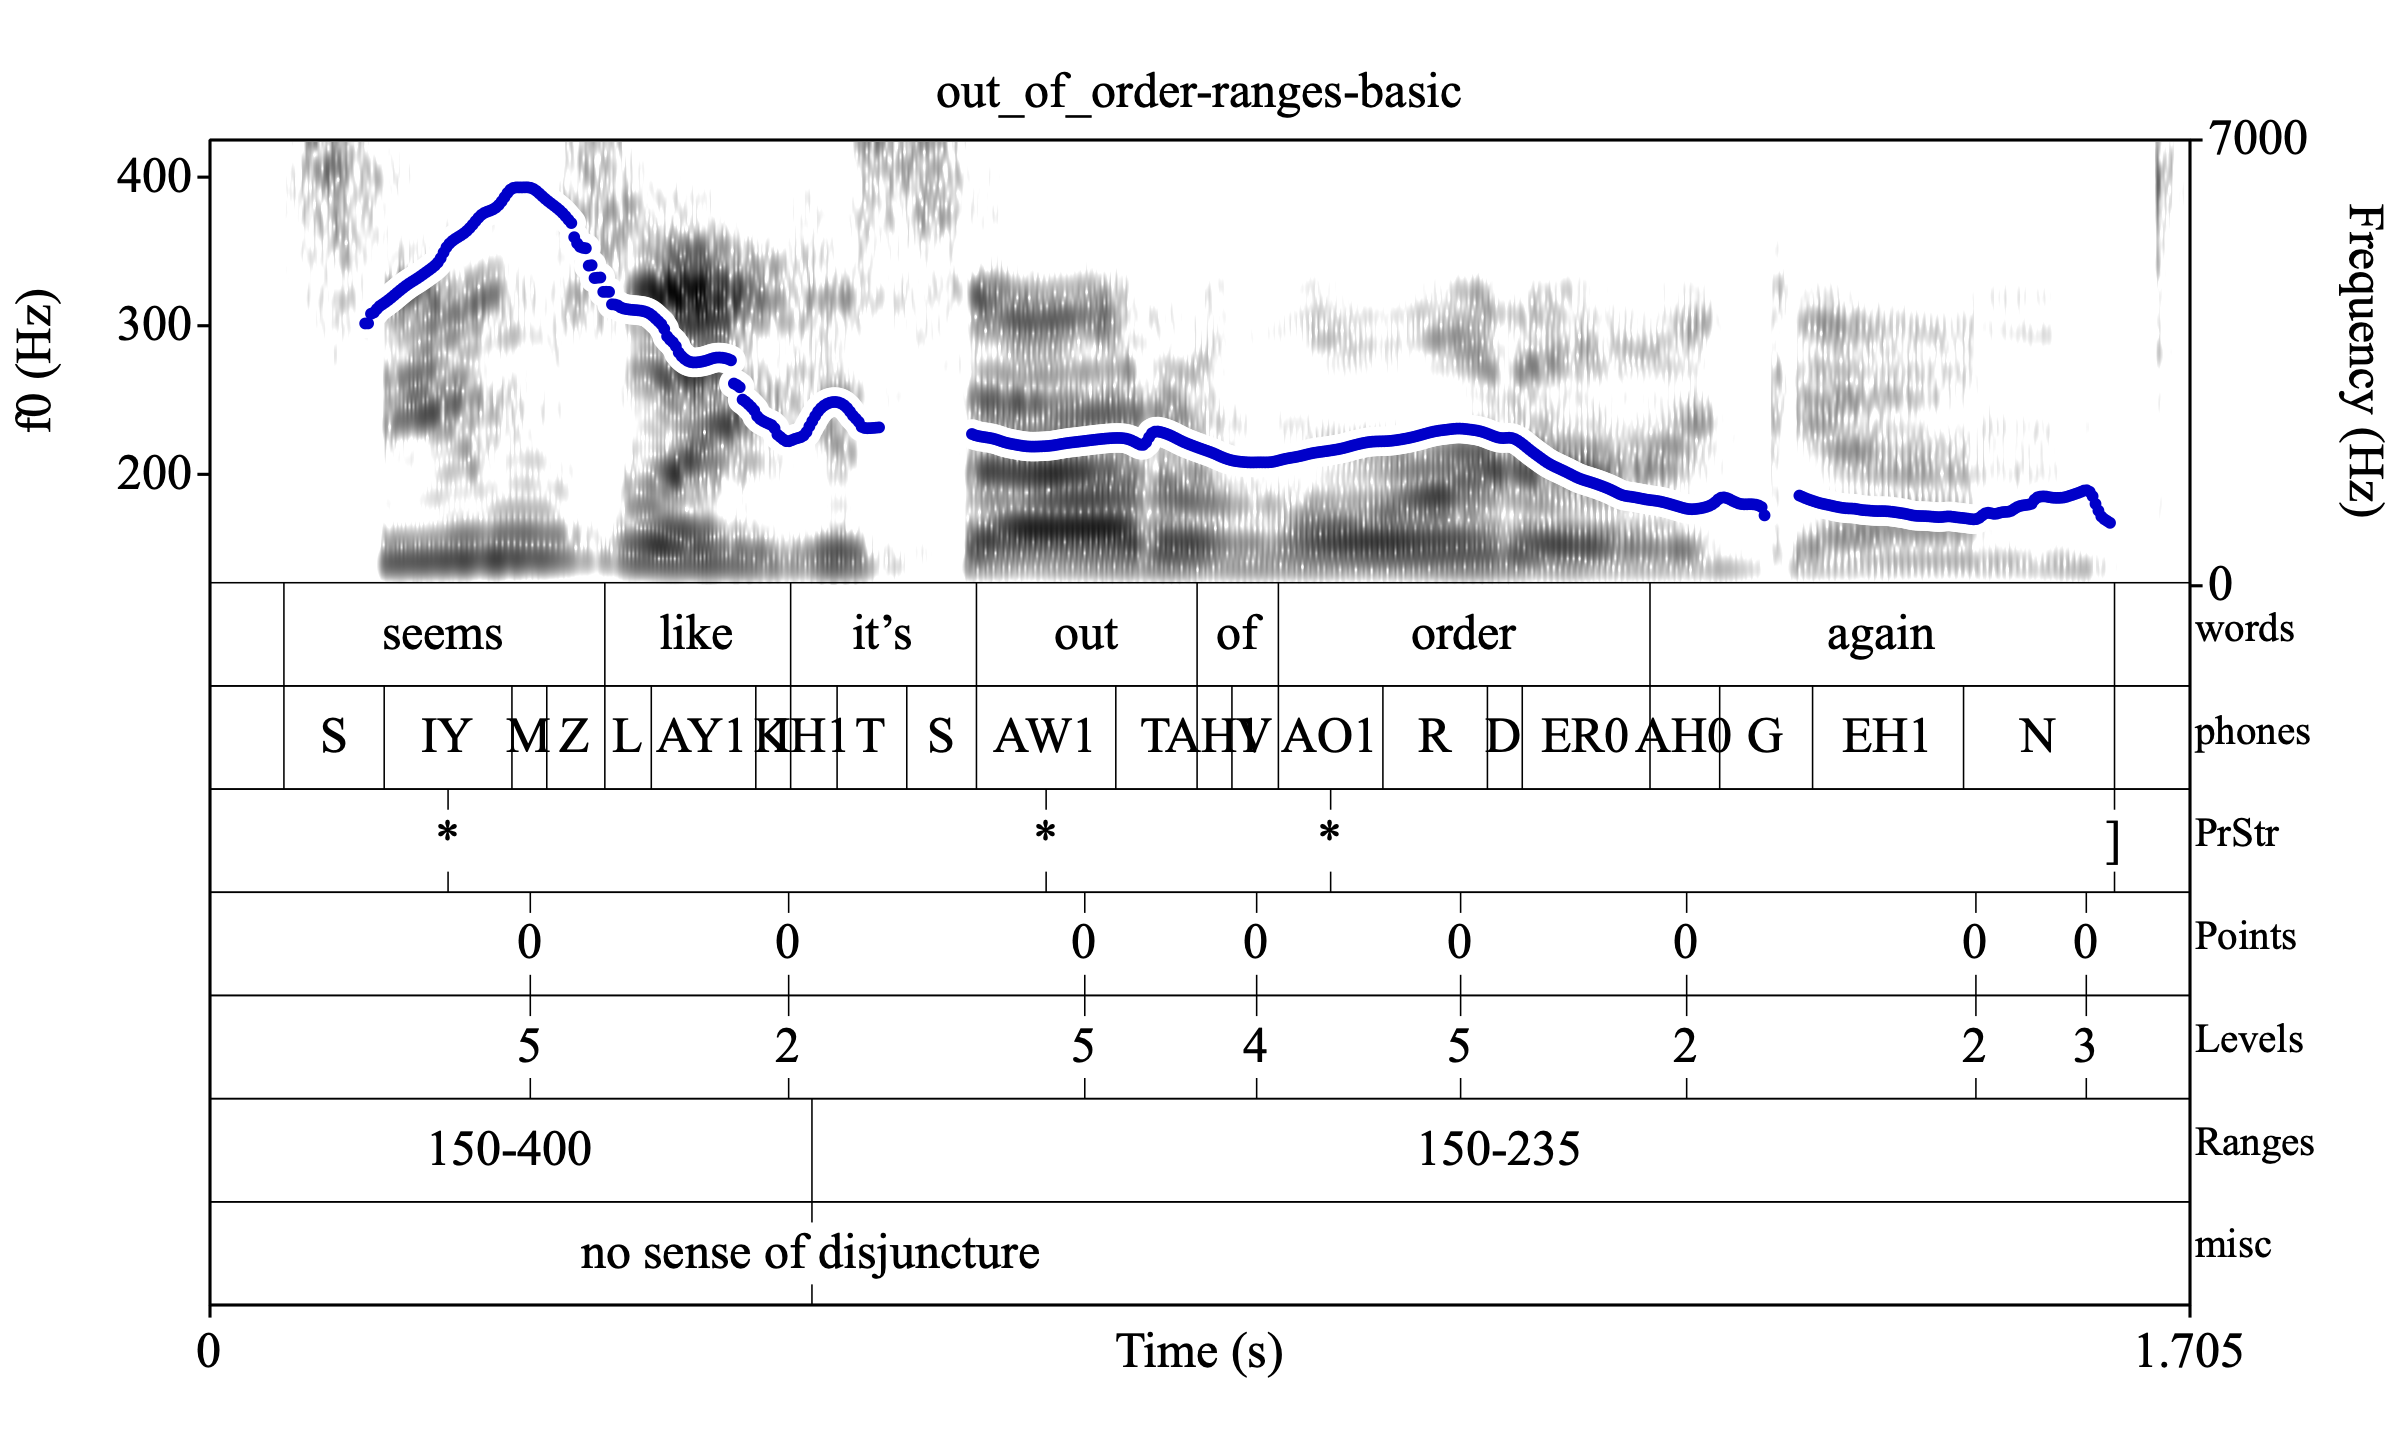
\includegraphics[width=.875\linewidth]{out_of_order-ranges-basic--7.png}
%
\caption{A recording annotated with Basic PoLaR labels. Note that the Phones tier is created automatically by the Montreal Forced Aligner (\citealt{mcauliffe-19}).\protect\footnotemark%
\label{fig:PoLaR 1st basic}%
\index{Annotated example, PrStr tier (basic)!out\_of\_order-ranges}
}
\end{figure}\footnotetext{The inclusion of a Phones tier does not reflect the authors’ commitment to the idea that phones have representational reality as bounded linguistic constituents.}


There are four core tiers of prosodic annotation (the third through sixth tiers in Figure \ref{fig:PoLaR 1st basic} above), described in these guidelines: three acoustic tiers (Pitch \textbf{Po}ints, Scaled \textbf{L}evels, \textbf{a}nd \textbf{R}ange Domains), and one phonological tier (Prosodic Structure).

\begin{enumerate} \def\labelenumi{\arabic{enumi}.}
\item The \uline{Prosodic Structure (PrStr) tier} is a point tier, and each label indicates the presence of a perceived prosodic prominence or a perceived prosodic phrase boundary. Prominence labels are placed in the middle of the vocalic nucleus of a prominent syllable, and boundary labels at the end of the last word of a prosodic phrase.
\item The \uline{Pitch \textbf{Po}ints tier} is a point tier, and each label corresponds to a turning point that the labeller observes in the f0. “Turning point” refers to any point in the f0 curve that looks to be a place where the f0 curve’s slope changes significantly (i.e., peaks, valleys, and the edges of plateaus).\footnote{PoLaR emphasizes the labelling of f0 turning points, because they are important aspects of an f0 contour, but this does not imply a commitment to an equivalence between turning points and intonational targets. See section \ref{sec:TCoG} on Tonal Center of Gravity for further discussion.} PoLaR also permits labellers to \textit{optionally} annotate, for each f0 turning point, which (type of) phonological object from the Prosodic Structure tier it is associated with. This tier is the aspect of PoLaR that requires the most substantial discussion, in part to establish which slope changes are significant, what types of ‘decoy’ or apparent f0 turning points can be ignored, and how missing turning points can be inferred; see section \ref{sec:points} for this discussion.
\item The \uline{Scaled \textbf{L}evels tier} is a point tier, and has a 1-to-1 relationship with the Points tier, in terms of the number and time alignment of annotations. That is, for each point in the Points tier, a point is added to the Levels tier, and that Levels tier object is labelled with a numerical value that corresponds to where in the current pitch-range (see 4 below) the turning point is. This tier is \textbf{automatically derived} from the Pitch Points Tier and the Range Domains tier, using the Levels labeller function of the PoLaR plugin for Praat.
\item The \uline{\textbf{R}ange Domains tier} is an interval tier, which captures a local pitch range for each utterance or section of an utterance. This annotation makes it possible to define the “high” and “low” for a particular stretch of an utterance, which is more explicitly manifested in the labels of the Scaled Levels tier (as in 3 above). For Basic PoLaR labels, the max\slash min for each Range interval is used to determine the numerical Levels values automatically inserted in the Levels tier. \end{enumerate}

Some PoLaR labels are phonological in nature (though also somewhat underspecified; e.g., “prominence” or “phrase boundary”), while others are more phonetic (e.g., f0 turning points). Annotating each tier only requires attention to one stream of suprasegmental properties (e.g., the Points tier only identifies f0 turning points); this allows each tier to be annotated on its own.\footnote{Note that no tier requires bundling information from multiple prosodic domains into a single label (this contrasts with a label like \textlabel{H*}, which bundles together prominence, pitch height, f0 turning points, etc.). Some Advanced labels re-connect these separated-out features; this is discussed at length for the Points tier in Chapter \ref{ch:advanced}.\label{fn:no bundling}}

PoLaR thus \textit{\uline{explicitly}} annotates both categories (phonology) and acoustic cues (phonetics), but with these streams of information \textit{\uline{separated from one another}}. We believe that annotating this information separately will reduce confounds in analysis and uncertainty in labellers. As we will see when discussing each tier in more detail, Advanced labels can be used to relate information on the phonological tier to information on the multiple phonetic tiers.

\subsection{Why These Tiers?}\label{sec:why-these-tiers}

The design choice of all labels and tiers (even these more phonetic ones) is, to some degree, phonologically informed and language-specific. That is, PoLaR labels do not identify just “any old (phonetic) information”, but rather information that is likely to be relevant for models of English intonation: e.g., pitch alignment, pitch height, prominence, and pitch range. These tiers and labels were chosen by the designers of PoLaR, based on experience with English intonation, but researchers who want to use PoLaR in another language may need to recalibrate the specific labels and/or tiers that get implemented. Because PoLaR is a framework for exploring the categories and cues to intonational prosody, rather than a fixed set of elements to be labelled, the number and nature of the tiers is extendable to accommodate the needs of particular studies. The following paragraphs review the thinking behind the design choices for each tier.

\uline{PrStr:}\\ Following AM theory (cf. \citealt{pierrehumbert80}), we assume that there are different types of intonational events, which are associated with different types of abstract phonological objects. In particular, we assume the now classic view that there are two basic sorts of phonological objects in prosodic structure that have direct influence of intonational contours: those related to intonational prominence and those related to intonational phrasing. (To be clear, the term ‘intonational prominence’ is meant to invoke a level of ‘post-lexical’ prominence: prominence higher than the level of lexical stress; cf. \citealt{bolinger58}, \citealt{libermanprince77}, and \citealt{beckmanedwards94}.) By design, all of the labels on this tier avoid indicating anything about how they are acoustically realized tonally - even abstractly. For example, differences like \textlabel{H-} vs. \textlabel{L-}, or \textlabel{H*} vs. \textlabel{L*} are purposely not captured at all in these labels. (These f0 properties will be captured by other labels on other tiers.) While these phonological objects can be signalled by a variety of cues (including changes in f0, duration, intensity, voice quality, etc.), none of these cues are themselves described by labels on this tier. Instead, what is transcribed is only the labeller’s \textit{\textbf{perception}} of prominence and phrasing. In this way, these Prosodic Structure tier labels are intentionally agnostic about the range of potential acoustic realizations of these different phonological objects. This method encodes information similar to that encoded by \citeauthor{cole-14}’s \citeyear{cole-14} Rapid Prosody Transcription method (RPT), and was influenced by their proposal. In RPT tasks, listeners mark perceived boundaries and prominences without concern for precisely how they are realized. This means that data gathered with an RPT methodology could be automatically translated into the accent and boundary tone markers on the Prosodic Structure tier. Labelling PrStr is designed to be simpler than other prosodic labelling systems, with the goal of allowing others to more easily understand the original labeller’s intentions.

\uline{Points:}\\ The f0 turning points in an f0 contour play an important role in many different theories.  For example, researchers have attributed a relationship between f0 turning points and phonological elements, either directly (e.g., as peaks, valleys, or anchored elbows; see, e.g., \citealt{ladd-99} and \citealt{welby06}) or indirectly (e.g., as important factors in implementing f0 shape and alignment distinctions, as in the Tonal Center of Gravity work of \citealt{barnes-12} et seqq.). For these reasons, it is useful to determine where they are.  Unfortunately, at the moment this cannot be done automatically, but requires human intervention, for several reasons.  First, f0 is challenging to track automatically, and there are often “missing” turning points (e.g. during voiceless segments or creaky-voiced regions).  Second, it is challenging to determine which turning points are significant, and which should in contrast be regarded as ‘decoy’ points: either too small to make a perceptible difference, or the result of a tracking error.  Thus, human labelling of points defined as significant for perception of intonation is required, and this monograph provides guidance for determining significant turning points, identifying decoys and inferring missing points.  See section \ref{sec:optional-f0-override-labels-for-annotating-pitch-points-without-a-reliable-f0-track} in Chapter \ref{ch:basics} for further discussion.

While it is widely agreed that there is a mapping relationship between the types of objects in our Prosodic Structure tier and the f0 turning points of the Points tier, PoLaR does not commit its labellers to any particular analysis of this relationship. In this way, the labeller need not try to keep the phonological model in mind while labelling the Points tier, nor even be familiar with any phonological model. At the same time, PoLaR provides a way for labellers to annotate the relationship between the two tiers. (How to do this is laid out in Section \ref{sec:optional-advanced-labels-for-relating-points-tier-objects-to-prosodic-structure-tier-objects} in Chapter \ref{ch:advanced}.) In this way, the Points tier can also be used for annotating mappings between acoustic events and phonological objects.

\uline{Levels:}\\ The Levels tier allows PoLaR to capture the relative height of a Points tier object (on a scale of 1 to 5). This relative height can be useful for analysis, since a raw f0 value does not by itself indicate whether that value is high or low (in the speaker’s current intended range). This is because, as noted earlier, a relatively low f0 in the speaker’s full possible f0 range may be functionally\slash phonologically high if the speaker’s current f0 range is low, and vice versa. The Levels tier encodes scaled pitch values for each f0 turning point on the Points tier. That value corresponds to the pitch quintile in which it occurs (1 being the lowest quintile and 5 being the highest), with the boundaries for each pitch quintile being calculated on the basis of the pitch range annotated in the Ranges tier. Annotators should use the PoLaR plugin for Praat to automatically have Levels annotation added, once Points and Ranges tiers have been annotated. Further discussion can be found in chapter \ref{ch:practical}.

\uline{Ranges:}\\ The Ranges tier reflects that f0 events are always interpreted within a speaker’s range--not only their overall speaking range, but within locally determined ranges. The Ranges tier provides the context in which the levels (i.e., on the Levels tier) reflect individual points on the Points tier. That is, this is used to identify whether an f0 point is “high”, “low”, or somewhere in between, in the context of a particular utterance or part of an utterance. The Ranges labels require human labellers because we need intuitions on which parts of the pitch are perceived to be H or L in the speaker’s range. The Ranges tier can be used to capture and reflect the relations and differences among pitch events, both locally within a range, and across ranges.

Labelling Ranges tiers in this way allows analyses that other AM labelling systems do not: relative heights between pitch ceilings\slash floors in arbitrarily distant parts of the recording can be compared. In AM labelling systems, the pitch range can only be inferred by looking at the labelling and the recording together, alongside a theoretical model of the relationship between phrasing and acoustic measures (e.g., that new intermediate phrases begin new pitch ranges). Such an inference can lead to problems in cases where the labeller and the reader have different assumptions about the relationship between phrases and pitch ranges. This highlights the PoLaR system’s core, laid out in the introduction: it keeps track of information that other intonational annotation systems make use of, but differently from those other systems, it requires that such information be tracked \emph{explicitly}.

\section{Overview of PoLaR’s Advantages}\label{sec:overview-of-PoLaRs-advantages}
Before delving into the details of the system, we describe here several general points about the advantages of PoLaR. Its primary goal is to identify the melody of a spoken utterance; in this sense it has something in common with the IPO approach (so named for the Dutch the Institute for Perception Research, ‘Instituut voor Perceptie Onderzoek’), which produces straight line approximations by connecting turning points (\citealt{t-hart-90}), which can serve as a proxy for key aspects of the melody.  In particular, PoLaR has been designed to have five useful characteristics: Compatibility, Flexibility, Modularity, Accessibility, Expandability, Crosslinguistic usability, and Explicitness; in addition, it has inspired concomitant development of a useful set of Associated Tools. 

\paragraph{Compatibility with other annotation systems / prosodic analyses:}
PoLaR works well with other labelling tools and systems which have different goals, and its use alongside other annotation systems is encouraged; PoLaR is not intended as a complete model of spoken prosody.  For example, parallel PoLaR and e.g. ToBI\footnote{ToBI annotation systems exist for a number of languages and varieties; see \citealt{jun05, jun14} for works describing ToBI systems for a number of languages.} labels can be expected to shed light on both the phonemic inventory of a language and the phonetics-phonology interface. 

For these reasons, PoLaR is not intended as a replacement for other annotation systems. As such, PoLaR can be seen as a supplement to existing systems (such as the ones mentioned in Section \ref{sec:past-approaches-to-prosodic-labelling}). At the same time, it can stand alone, and PoLaR labellers need not have any familiarity with other prosodic annotation systems.

\paragraph{Flexible for different research goals:}
The PoLaR system, which builds on existing frameworks and labelling systems, was developed to enable both (1) more detailed descriptions of languages with well-studied intonational phonology, in particular with reference to the capture of acoustic details of intonation for which the linguistic relevance has not yet been determined, and (2) the annotation of phonetic patterns in languages, dialects, or varieties whose phonology has not yet been explored, as a step toward understanding the intonational grammar. Its minimal invocation of language-specific phonology adopts prominence and boundary locations from AM theory, and it focuses on acoustic characteristics that are, according to human judgment, relevant for linguistic signalling (\citealt{barnesshattuckhufnagel20}).   

At its core, a PoLaR annotation is a phonologically-informed (but maximally theory-neutral) labelling of intonational acoustic-phonetic cues. This description brings to the forefront the fact that PoLaR labels are neither purely phonetic, nor purely phonological; instead, they are intended to capture phonologically relevant acoustic aspects of the speech signal. Thus, what is perhaps most important here is the separation between labels for phonological objects from phonetic labels of the acoustic characteristics that serve as cues to those objects, as well as the separation of different acoustic cues each to its own tier, and explicit labelling of more of these acoustic characteristics. We believe the labels that we provide below for each of the proposed labelling tiers are a good starting point for US English varieties, but exemplify what PoLaR annotation can do for any language or variety.

\paragraph{Modularity / “Unbundled” labels:}
In PoLaR, acoustic-phonetic cues and phonology are annotated separately. (And the phonological labelling is minimal, specifying (in its basic form) only the location of prominences and boundaries.) This reflects design principle: PoLaR \textbf{disentangles different types of information} as much as possible - isolating different components of prosody on different tiers of annotation. This unbundling facilitates decision-making during labelling, by requiring only minimal phonological awareness on the part of the labeller. (This stands in contrast with phonological labels that bundle together prominence, pitch alignment and scaling, etc.) This unbundling allows PoLaR to be annotated one at a time (at least with the Basic labels in Ch.\ref{ch:basics}), without the need to consider the labels on other tiers - this allows for a ‘divide and conquer’ approach to the labelling task, in which individuals can specialize in specific tasks, in an assembly line model.

At the same time, for those advanced labellers who are interested in connecting labels to a prosodic theory, PoLaR also provides ‘Advanced’ labels (Ch.\ref{ch:advanced}), to allow a labeller to annotate some relationships between tiers. This may facilitate exploration of how prosodic components on one tier relate to components on another. (See Extensibility below.)

\paragraph{Accessibility of use:}
PoLaR has been designed to be \textbf{easy to start using}, with relatively minimal instruction, so that useable data of particular interest to a researcher can be produced quickly.  This is in part because PoLaR does not require its labellers to have extensive knowledge of a phonological model of prosody, and in part because the different sets of labels are inherently module (allowing some labellers to be only trained in one area of prosodic labelling).

PoLaR’s modularity and lack of reliance on prosodic phonology stands in contrast to existing systems which do not specify how precisely to map labels onto particular sets of cues, and thus do not enable straightforward investigation of how different speakers (and labellers) use different cues in different contexts, or of what cues speakers use to signal particular contrastive intonational categories.

Because of this accessibility, the tasks of labelling different tiers can be split among different labellers, who can quickly develop expertise in that area.  In this way, the first steps of the labelling process are intermediate between the full training process for phonological labelling and the training-free method of Rapid Prosody Transcription (RPT) described in \citet{cole-14, cole-17}. 

Moreover, while accessible, the system requires that annotators using even the most basic PoLaR labels be explicit about their perception, intuition, and/or analysis - facilitating high-level discussions among more experienced or analysis-oriented users. (In addition, Advanced PoLaR labels allow such analysis-oriented users to systematically transcribe their analyses.)

\paragraph{Expandability of the annotation system:}
Although this monograph focuses on the \emph{intonational} aspects of spoken prosody, a critical feature of PoLaR’s design is that it does not restrict labellers to only annotating this information. To be clear, we mean that PoLaR annotation is broadly intended as a \emph{\textbf{framework}} (which is to say it is a way of conceptualizing annotation systems), so that there is not a rigid way for PoLaR annotation to be implemented. 

Instead, the particular implementation described in this monograph is intended to be seen as a narrow execution of broader conceptual ideas. A labeller can expand\slash contract the set of labels on a particular tier or expand\slash contract the set of tiers that are labelled, so as to adjust what aspects of prosody and cues to prosodic structure are annotated. For example, a labeller may wish to systematically annotate duration, intensity, or phonation cues. Or they may wish to annotate other aspects of prosodic structure, such as lexical stress, footing, etc. This is useful, because tabulating and understanding the individual cues to prosodic prominences and boundaries can provide important insights into how phonetic implementation of a phonological intonation category can vary (\citealt{brugos15, brugos-18}).

Labelling projects with different goals can also omit tiers that are judged to be less relevant, allowing a novice labeller to focus on (and become expert in) a particular aspect of the intonation.  In this way, more complex labelling tasks can be approached with a divide and conquer strategy, which allows each labeller to become expert and reliable more quickly. 

\paragraph{Crosslinguistic usability:}
PoLaR is designed to be usable for any language as well as for any speech style, register, or dialect \emph{within} a language. PoLaR’s focus on acoustic cues and broad phonological categories makes PoLaR useful in the initial stages of exploring a language or dialect whose prosody is under-\slash un-documented.  While some tiers require native speaker intuition (e.g., prominences, boundaries). others could be used without native speaker intuitions (e.g., turning points).  Thus, using PoLaR can be a step toward formulating a phonological transcription system of intonationally-undocumented systems.  This is critically important, because our current understanding of human speech prosody is based on analysis of a strikingly small proportion of the world’s languages, while at the same time, it has become easier to create corpora of recorded utterances in understudied languages for analysis.  Thus the time is right for development of a system such as PoLaR which facilitates getting a foothold on the analysis ladder for addressing a new language or dialect. 

Beyond work on understudied languages\slash dialects, PoLaR can also be useful for studying how suprasegmental cues are used differently across varieties and contexts, within a language\slash variety. Researchers working with a corpus that is annotated for demographic or contextual information could use PoLaR labels in much the same way as it would be used for crosslinguistic work.\footnote{For those wishing to create their own corpus, see, e.g., \citealt{meyerhoff-11} or \citealt{podesvasharma13} for some discussion of recording this sort of information as well as a description of some best practices.}

\paragraph{Explicitness of annotation:}
PoLaR facilitates discussion with respect to differences in labeller intuitions, through its explicit annotation of cues (such as f0 turning points and ranges). Discussions are also facilitated through the relationships described by Advanced labels, which can encode labeller intuitions about the connections across tiers (such as pointers in the Points tier to indicate the direction of affiliation to a phonological boundary or prominence). Similarly, it encourages the development and testing of hypotheses about systematic aspects of these relationships. For example, PoLaR facilitate analyses that reveal not only how each type of prominence and boundary proposed in a phonological theory of intonation can be realized acoustically in different contexts, but also whether the proposed contrastive categories would benefit from extension or revision.

\paragraph{Associated tools:}
A plugin has been developed that includes a set of scripts to facilitate the labelling process. (As described at several points throughout this monograph; it can be accessed through the OSF repository at \url{https://doi.org/10.17605/OSF.IO/USBX5}.) This plugin can do things such as helping a labeller determine whether a particular PoLaR label ought to be included, substantially facilitating the resolution of ambiguous cases. Other functions include automatically adding labels on particular tiers on the basis of other labels, and exporting information extracted based on the labels in a format that can be usable for statistical analysis and machine learning.  (For more discussion of this plugin, see Chapter \ref{sec:past-approaches-to-prosodic-labelling}.) Finally, the system benefits from integrating with existing tools, such as ones for phone segmentation by forced aligners (e.g. Montreal Forced Aligner, \citealt{mcauliffe-19}, downloadable from \href{https://github.com/MontrealCorpusTools/Montreal-Forced-Aligner}{MontrealCorpusTools on Github}; or the Penn Forced aligner, \citealt{yuanliberman08}, downloadable from the \href{https://web.sas.upenn.edu/phonetics-lab/facilities/}{Penn Phonetics Laboratory website}).

%todo add a section on places to be concerned?
% reviewer note:
%My second point is a methodological one regarding interrater reliability between labellers. The fact that the advanced version of PoLaR is very rich in its inventory and provides a wide range of possibilities for annotation (integration / linking of events etc.) makes it complex at the same time. My question is how well the system can be learned and how reliable annotations across annotators are (especially with regard to the Ranges Tier, see above). I think that a framework as comprehensive as PoLaR needs to provide the reader with information on such issues. It is a plus that PoLaR can be used by both novices and advanced labellers and that the book can be read selectively. Adding a chapter on interrater reliability studies (for both the basic and advanced approach) would substantially strengthen the manuscript and the annotation system as a whole.
	%> response: there are many places of labeller freedom that can yield problems, yes; ADVICE: researchers could document choices?



\section{Who Will Find PoLaR Useful}\label{sec:who-will-find-polar-useful}

This monograph describes a recently developed system for annotating prosody, PoLaR, which is  aimed at fulfilling some of the needs described above. PoLaR has been designed with some particular influences and goals in mind, as outlined in the next section. Before getting into the details of those goals, and how they differ from the goals of other annotation systems, we will suggest some circumstances in which we think PoLaR might be particularly useful.

\textbf{How much experience is required to become a user?} PoLaR has been designed to facilitate the labelling process, and to be useful for a wide range of individuals with different levels of experience, backgrounds, and goals. It is designed to require minimal theoretical knowledge, enabling \uline{novice labellers} to begin producing useful annotations more quickly. It is also designed for research groups where different individuals label different aspects of the signal, \uline{in parallel}. Lastly, advanced aspects of the system are designed to be useful for \uline{advanced labellers} or \uline{theoreticians}, who are interested in the finer details of the prosody.

\textbf{Which areas of research could benefit?} PoLaR was also designed to facilitate making new discoveries, especially with respect to how variation within prosody (and specific prosodic characteristics) relates to variation in a (linguistic and/or extra-linguistic) context. For this reason (alongside its usability for novice labellers), PoLaR will be useful for \uline{variationists}, \uline{sociolinguists}, \uline{acquisitionists}, \uline{semanticists\slash pragmaticists}, \uline{morphologists}, \uline{phonologists}, etc. --as well as those working at the interfaces-- to help understand how prosody relates to these domains. Because it facilitates the annotation of potentially systematic aspects of the acoustic detail of an intonational contour, it is well suited to exploratory analysis of both understudied languages and understudied varieties of familiar languages.





%%%%%%%%%%%%%%%%%%%%%%%%%%%%%%%%%%%%
%%%%
%%%%     CHAPTER 2 getting started
%%%%
%%%%%%%%%%%%%%%%%%%%%%%%%%%%%%%%%%%%
\chapter{Getting Started with PoLaR}\label{ch:basics}

This chapter introduces PoLaR labelling, with labels that we call ‘Basic labels’ – ones that capture the essential core of this annotation system, but without much in the way of deep analysis. This chapter starts guidelines for annotating prosody with PoLaR labels in section  \ref{sec:labelling-polar-tiers}.\footnote{These guidelines represent version 1.0 of PoLaR annotation (\citealt{ahn-21}). Any developments beyond version 1.0 will be available through the PoLaR repository: \href{https://doi.org/10.17605/OSF.IO/USBX5}{https://doi.org/10.17605/OSF.IO/USBX5}, which is also home to sound files, PoLaR-labelled TextGrid files, and other resources.} Next, section \ref{sec:intonational-contours-and-software-based-pitch-tracks} walks through cases where there is pitch track disruption in software like Praat, and readers are provided tools to deal with such disruptions. More theoretically- and analytically-driven labels are described in the chapter following this one, but even readers oriented towards detailed analysis must start with this chapter first.

\section{Labelling PoLaR Tiers}\label{sec:labelling-polar-tiers}

This chapter is intended to be useful to people without any prior training in intonation. For these novice labellers, the Basic labels (described in this section) will be critical. At the same time, there are many labellers who are well versed in using other labelling systems but would find Basic labels useful on their own. This chapter describes how to get started with PoLaR, using what we call “Basic” labels. The Basic labels embody the core spirit of PoLaR labelling: un-bundled labels (in the sense described in section \ref{sec:overview-of-PoLaRs-advantages}) about different prosodic aspects of the speech stream.

(\textit{Chapter \ref{ch:advanced} describes “Advanced” labels that build on an understanding of the Basic labels. Advanced labels allow experienced labellers to include more of their intuitions about relations between tiers, to be explicit about connections to prosodic theories, and to deal with more complex situations.})

The PoLaR annotation framework consists of four core tiers, with the option for labellers to add more tiers to suit their particular needs. Each of these four core tiers will be discussed in turn, in sections \ref{sec:prosodic-structure-prstr}-\ref{sec:levels}.

Before we go into more depth on the particulars of the labels in each of these tiers, we summarize the general labelling process. The Prosodic Structure, Points, and Ranges tiers are annotated by human labellers, who can do so with only minimal amounts of training. Because different prosodic characteristics are separated on different tiers, labellers can easily focus on one tier / one characteristic at a time. Moreover, labelling some tiers may not even require training (cf. Rapid Prosody Transcription, developed by \citealt{cole-14}). Thus, the labelling task can be more easily split amongst a team of labellers (including prosodic novices) by directing each member to attend to only a subset of characteristics. Finally, a computer algorithm can be used to automatically generate the labels for the Levels tier, on the basis of labelled Points and Ranges tiers. This algorithm has been implemented as a Praat script (bundled in a plugin; see following paragraph). Future developments may lead to additions of similar sorts of automated labelling, once a large enough corpus of PoLaR labels has been collected so as to allow computational modelling between raw acoustics and PoLaR labels.

In addition to the previously mentioned scripts, there are a number of other tools available to facilitate PoLaR labelling using Praat (a commonly used annotation and processing software package found at praat.org; \citealt{praat}). These tools are bundled in a Praat plugin, which can be found at \href{https://doi.org/10.17605/OSF.IO/USBX5}{\uline{doi.org/10.17605/OSF.IO/USBX5}}, using the PoLaR OSF Repository link. Download the zip file named \texttt{plugin\_PoLaR} found in the repository and follow the instructions in the README file to add all of the currently available scripts to the praat editor window.

\subsection{Prosodic Structure (PrStr) Tier}\label{sec:prosodic-structure-prstr}

The Prosodic Structure tier encodes two types of elements, related to phonological prosodic structures: \textbf{intonational prominence} (high levels of stress) and \textbf{prosodic phrases} (groupings of words). When it comes to prominence\slash stress, let us be clear that we are referring to phonetic\slash phonological prominence (and not necessarily semantic\slash pragmatic prominence or communicative\slash cognitive prominence; cf. \citealt{gussenhoven15} and \citealt{wagner-15}). Under the umbrella of phonetic\slash phonological prominence, it is understood that there are different degrees. Let us first consider “lexical” levels of stress.\footnote{A note on terminology: “stress” is typically used in contexts of prominence of particular linguistic units (e.g., syllables and words) while prominence is a more generally applicable term.} In a word like “\langtext{Indianapolis}”, there are three levels of lexical stress represented. The highest level (primary lexical stress) is on the fourth syllable, “\langtext{na}”; the second highest level (secondary lexical stress) is on the first syllable “\langtext{in}”; and the lowest level (unstressed) can be found on the remaining four syllables. Lexical stress is \uline{not} something that we annotate here, since (in a language like English) lexical stress placement is generally recoverable from the identity of the word itself. (That is, “\langtext{Indianapolis}” has the same lexical stress patterns [described above] across contexts.) Because of this recoverability, annotation would be redundant.

There are higher levels of stress on top of lexical stress: what we will call “intonational prominence” (a.k.a., ‘post-lexical stress’, ‘phrasal stress’, or ‘accent’). Unlike lexical stress, having intonational prominence is much more context-dependent, depending on factors like the broader syntactic context and the details of the intended semantic\slash pragmatic meaning. Because of this, the same word may have intonational prominence in one utterance, but not in another (even if the sentence has the same words in the same order).

Consider these two utterances, both of which are transcribed as “\langtext{another greenish banana}”. In both cases, the same words are used (so the lexical stresses are in the same places). What differs between them is the location of the one intonational prominence in each. In the former, “greenish” is intonationally prominent, while in the latter it is “another”. Even without hearing the utterances, the visual f0 display shows a significant f0 rise-fall over the target words. 

\begin{figure}[H]
\centering
%
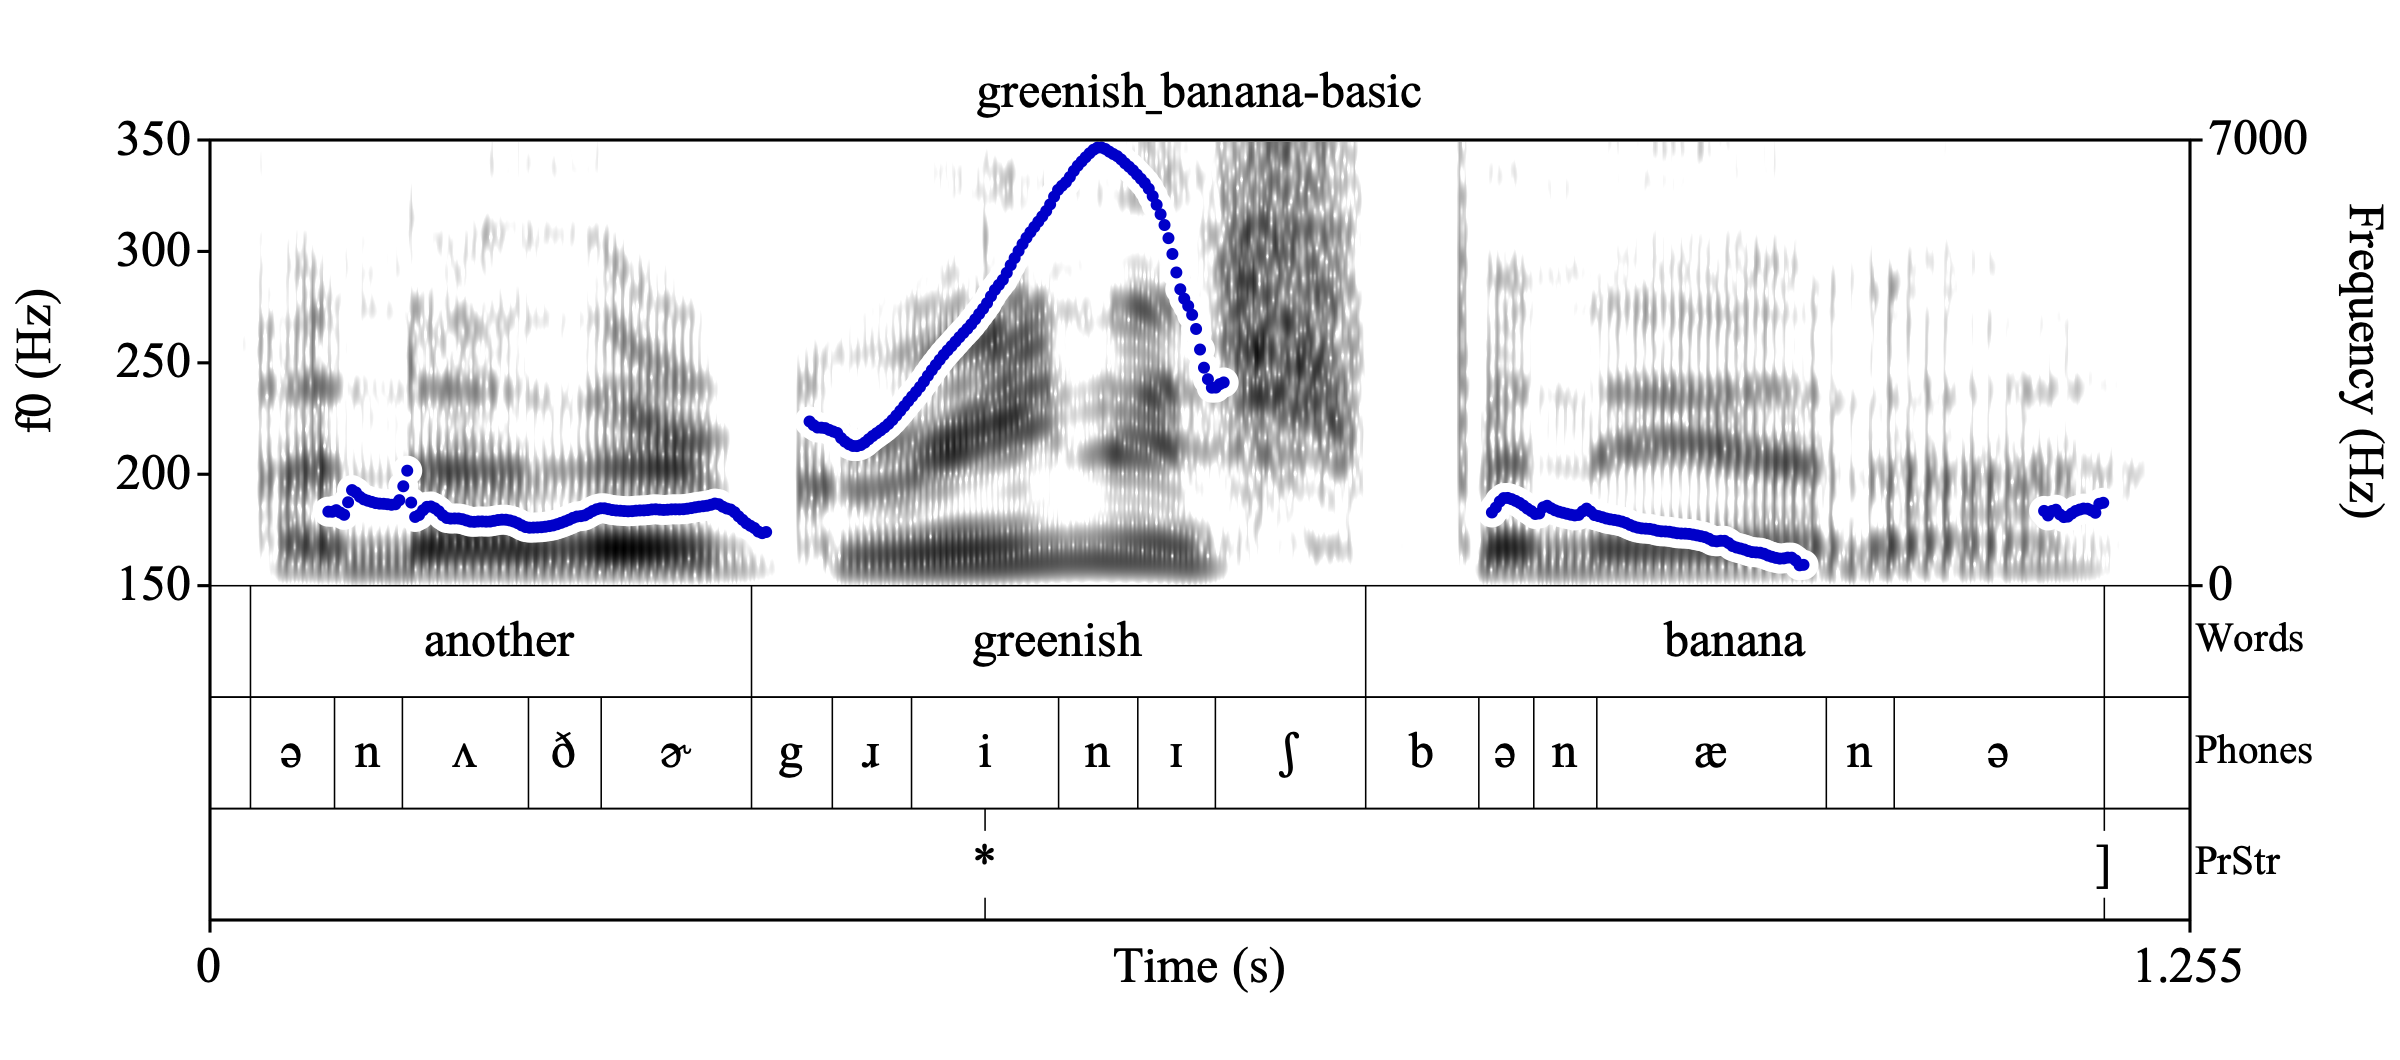
\includegraphics[width=.875\linewidth]{PrStr-greenish_banana-basic.png}
%
\caption{\texttt{greenish\_banana}: There is one prominent word, “greenish”.%
\label{fig:greenish banana prominent greenish}%
\index{Annotated example, PrStr tier (basic)!greenish\_banana}%
}
\end{figure}

\begin{figure}[H]
\centering
%
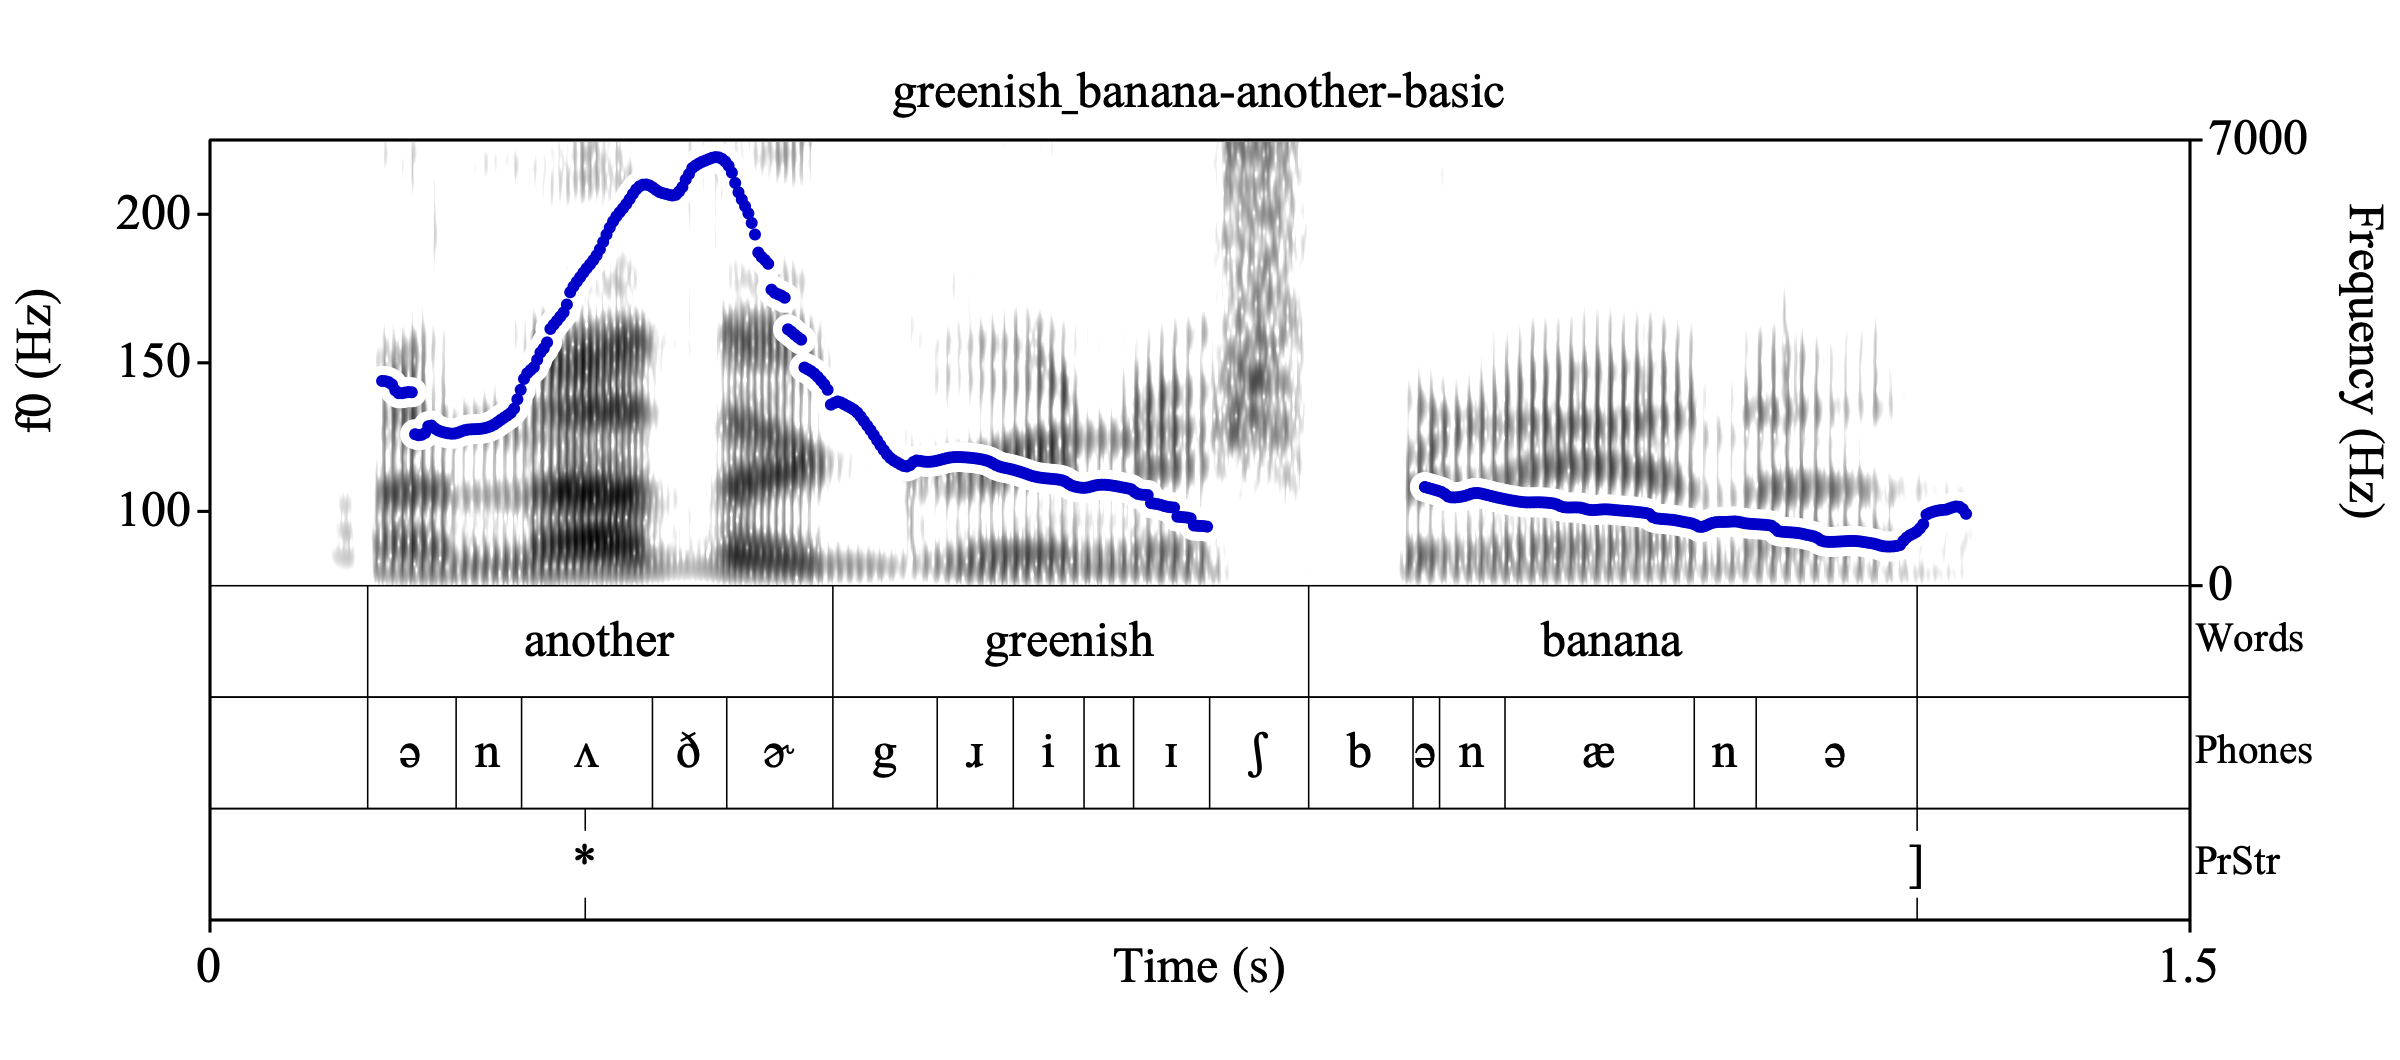
\includegraphics[width=.875\linewidth]{PrStr-greenish_banana-another-basic.png}
%
\caption{\texttt{greenish\_banana-another}: There is one prominent word, “another”.%
\label{fig:greenish banana prominent another}%
\index{Annotated example, PrStr tier (basic)!greenish\_banana-another}%
}
\end{figure}

\begin{infobox}[frametitle=\textbf{A NOTE ON PRAAT SETTINGS}]
If you follow along with these figures on your own machine using Praat (\citealt{praat}), there may be places where the figures in this monograph differ from the figures produced by your software. To minimize the number of differences, you can change the settings in your Praat to match those that are used to produce these figures. All figures in this monograph were created in Praat, using the “Draw Sound and TextGrid” functionality, which is a part of the PoLaR plugin for Praat. (\textit{This plugin can be found by going to \url{https://www.polarlabels.com}}.) This functionality is built on a script in which various settings related to pitch analysis and pitch display are specified – and these settings can radically affect how Praat identifies and analyzes pitch. These settings are given here: First, the Time Step analysis (found in \texttt{View>} Time step settings\ldots) was set to use a fixed strategy, at a time step of 0.0025s. Next, the “Advanced Pitch settings” (found in \texttt{Pitch>} Advanced pitch settings\ldots) were set as the following: Max. number of candidates=15, Very accurate=true, Silence threshold=0.03, Voicing threshold=0.5, Octave cost=0.05, Octave jump cost=0.5, and Voiced/Unvoiced cost=0.2. Screenshots of these settings windows are provided here: \par\begingroup\centering
	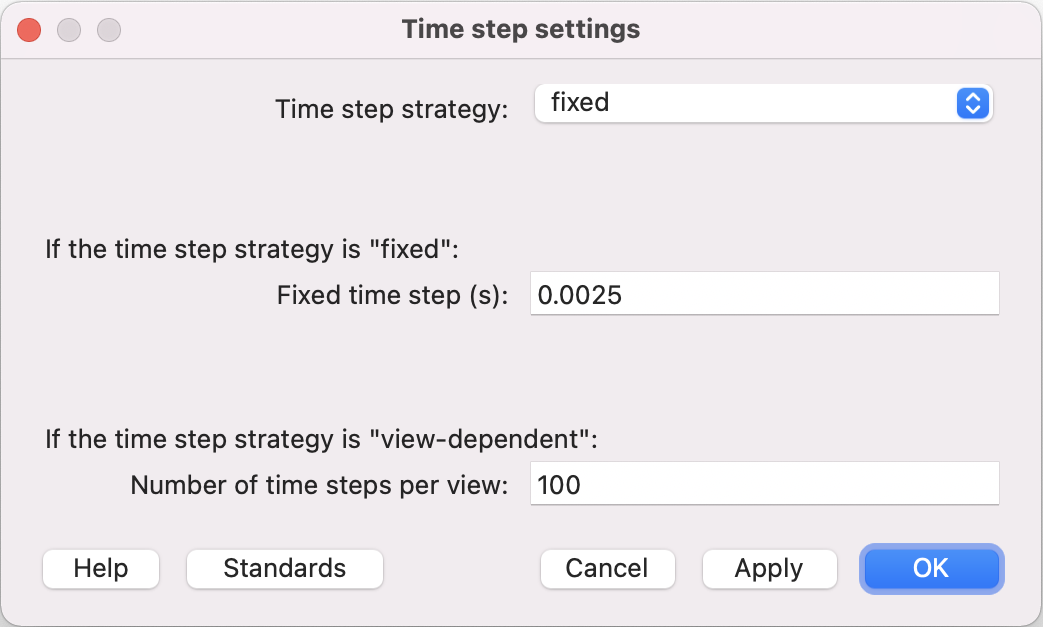
\includegraphics[width=.475\linewidth]{Praat-time-step-settings.png} 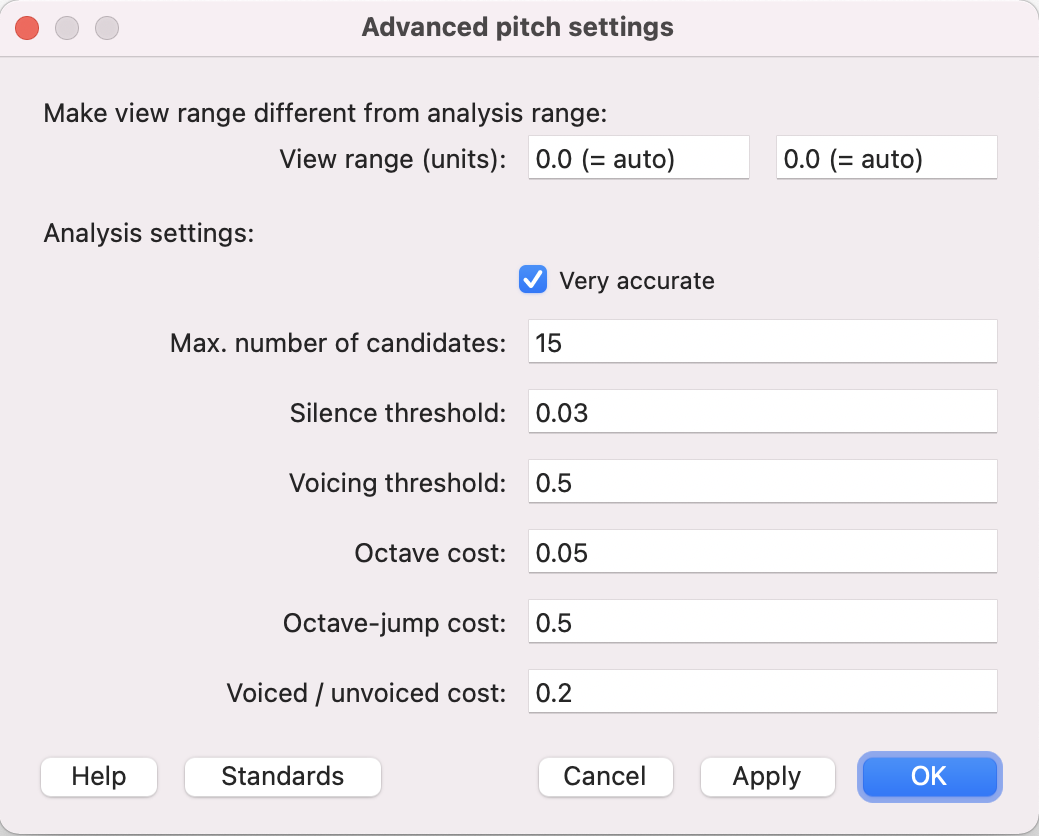
\includegraphics[width=.475\linewidth]{Praat-adv-pitch-settings.png} \par
	\endgroup (\textit{You may find it beneficial to adjust these settings further, to minimize pitch halving\slash doubling in particular recordings. However, doing so may result in pitch tracks that look different from the ones in this monograph.})
\label{note on praat settings}
\end{infobox}


It need not be the case that there is only one intonational prominence in an utterance; in fact, in many utterances with more than one content\footnote{So-called “content” words contrast with “function” words, where the former typically name concepts (e.g., “\langtext{human}”, “\langtext{energetic}”, “\langtext{remember}”) and the latter typically serve grammatical functions (e.g., “\langtext{the}”, “\langtext{itself}”, “\langtext{by}”, “\langtext{be}”).} word, it is common for there to be multiple words with intonational prominence. (There are plenty of examples of this throughout this monograph that show this, and more examples of PrStr labels are given in the “examples” section below.)

To annotate intonational prominence, we will adopt the \textlabel{*} symbol, from the AM tradition. In English, like lexical stress, intonational prominence is a phonological property associated with \textit{a syllable}, and so when we use the \textlabel{*} annotation, we want to align it in the Praat TextGrid with respect to the syllable that is perceived as prominent.\footnote{Prominence is realized with a number of acoustic cues, which may include increased amplitude, increased duration, one or more pitch movements, and hyperarticulation. At the same time, it is not the case that all of these cues are present for any given prominence. Moreover, across different contexts, any member of the set of cues may be weighted differently in their effect on perception of prominence. Finally, these cues only signal the intonational prominence and are not the intonational prominence itself. As such, instead of requiring that a PrStr tier labeller attend carefully to the cues (though they can!), PoLaR only requires that listeners consult their intuition that they perceive a given syllable as intonationally prominent.\label{fn:prominence cues}} This is shown in Figures \ref{fig:greenish banana prominent greenish} and \ref{fig:greenish banana prominent another}, on the third tier.

NOTE: Labellers are encouraged to adhere to consistent practices for the time-alignment of the \textlabel{*} labels. As an example of a regular practice for time-alignment, the present authors time-align their \textlabel{*} labels to the middle of (the segment that the forced aligner picks out as) the vowel\footnote{More accurately, we mean the middle of the “nucleus”, which is often realized as a vowel in English, but can also be realized as certain syllabic consonants (e.g., [n̩]).} of the syllable that is perceived as the intonationally prominent.\footnote{For a vast majority of cases, this syllable is the lexically stressed syllable of a word that is perceived as prominent – but not always (cf. certain cases of focus such as what is called “metalinguistic focus” in \citealt{erteschik-shir99} \textit{et seqq}, as well as other cases where contrastive focus can be found on other syllables as discussed in \citealt{armstrongschwenter16} and \citealt{ahn-21a}).}

Let’s now turn to prosodic phrasing. Phrasing refers to how words are grouped, so that some are perceived with no disjuncture between them (i.e., they are perceived as sounding closely grouped together), and some words are perceived as having (various levels of) disjuncture between them. Though pauses between words are one very strong cue to disjuncture, disjuncture is \uline{not} the same as pauses. (It can occur when there is no discernible pause between words, too.) Consider the following example, in which there is a perceived phrase boundary between “\langtext{beans}” and “\langtext{some}”, despite the fact that the /z/ sound at the end of “\langtext{beans}” leads right into the /s/ sound of “\langtext{some}”, with no pause:\footnote{Like prominence (see footnote \ref{fn:prominence cues}), phrase boundaries can be realized with a number of different acoustic cues. Cues to phrase boundaries may include a pause between phrases, changes in rate of speech production at the end of a phrase (and beginning of the next one), hyperarticulation at the beginning of a phrase, one or more pitch movements, changes in pitch range, and changes in voice quality. At the same time, it is not the case that all of these cues are present for any given phrase boundary. Moreover, across different contexts, any member of the set may be weighted differently in their effect on perception of phrase boundaries. Again, a PrStr tier labeller need not attend carefully to the particular acoustic cues (though they can!); instead, PoLaR only requires that listeners consult their intuition that they perceive a sense of disjuncture.\label{fn:phrasing cues}}

\begin{figure}[H]
\centering
%
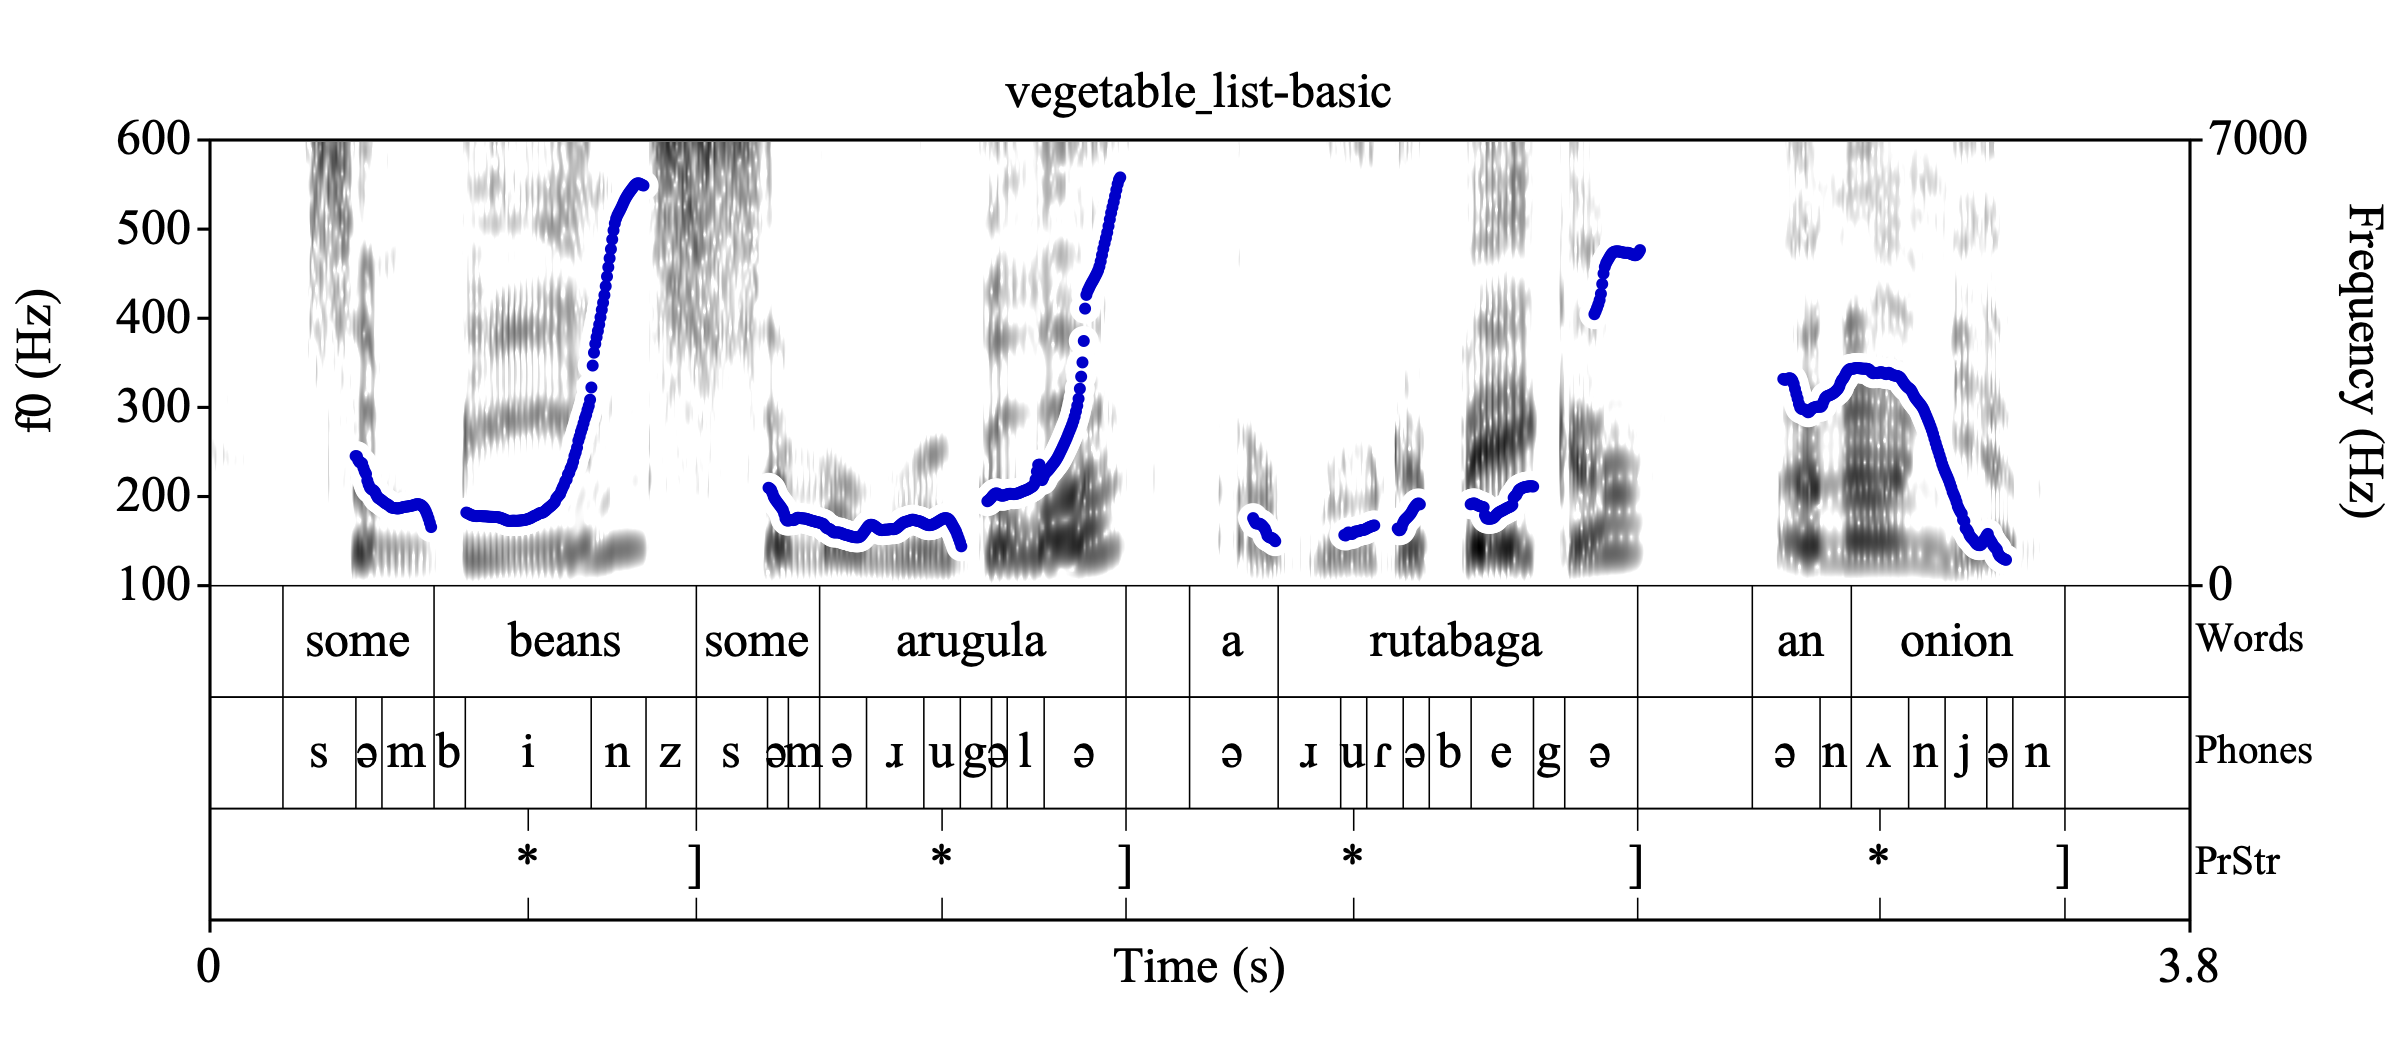
\includegraphics[width=.875\linewidth]{PrStr-vegetable_list-basic.png}
%
\caption{\texttt{vegetable\_list}: There are four prosodic phrases.%
\label{fig:vegetable list phrases}%
\index{Annotated example, PrStr tier (basic)!vegetable\_list}%
}
\end{figure}

Prosodic phrasing (like prominence) cannot be predicted solely on the basis of the words alone, but requires more knowledge about the context in which those words were spoken. In the example above, it is read as a list of four items, in four phrases; but you could imagine a context where the speaker was listing all the words on a page and then pronounces it as eight separate phrases (one for each word). Because phrasing is variable in this way (and because it has important effects on various suprasegmental properties), we annotate phrase boundaries explicitly.

To annotate prosodic phrasing in English, we will adopt the convention from the AM tradition of only annotating the boundary at the end of a phrase. (The idea is that the end of one phrase coincides with the beginning of another.\footnote{This is not a given for all work on prosodic phonology. As such, in the Advanced labels chapter, we describe a means of labelling other boundary edges.}) We will use the \textlabel{]} symbol for this. The end of a phrase is typically aligned with the end of a word, and so when we use the \textlabel{]} annotation, we want to align it in the Praat TextGrid with respect to the word boundary of the phrase-final word. Refer to the third tier of the Figure \ref{fig:vegetable list phrases}, to see this. Because basic PoLaR labels only indicate where a phrase ends, in cases where there is a pause after a phrase (e.g., after “\langtext{arugula}” or “\langtext{rutabaga}” in Figure \ref{fig:vegetable list phrases}), the \textlabel{]} label is placed before the pause. (Again, for more examples of this PrStr labelling, more examples are given throughout this monograph and in the “examples” section below.)

\subsubsection{Prosodic Structure Transcription}
To summarize, the two labels we have seen so far are described in Table \ref{2 PrStr basic labels}.

\begin{longtable}{cll} \toprule \textbf{Label} & \textbf{Phonological Object} & \textbf{Label is time-aligned with \_\_\_\_\_}\tabularnewline
\midrule \endhead
\textlabel{*} & Prominence & A syllable that has intonational prominence \tabularnewline
\textlabel{]} & Phrase’s Right Edge & The right edge of the final word of a phrase \tabularnewline
\bottomrule 
\caption{Two Basic labels for the Prosodic Structure tier (for English).%
\label{2 PrStr basic labels}%
}
\end{longtable}

(\textit{For labellers who wish to annotate more fine-grained levels of phonological analysis,}\footnote{For example: different types of prominence (nuclear stress, pre-\slash post-nuclear stress, focal stress, etc.), and different types of phrases (intermediate\slash phonological phrases, intonational phrases, etc.) or different phrase edges (i.e., the left edge of a phrase).} \textit{there are optional Advanced labels for this tier as well, which are described in Chapter \ref{ch:advanced}.})

\begin{infobox}[frametitle=\textbf{A side-note about this tier}]
This tier is called “Prosodic Structure”, and contains labels that refer to elements of that structure that are relevant for intonational annotation. There is more to prosodic structure than has been described here; e.g., the labels described until now do not annotate lower levels of structure (e.g., syllable structure, lexical prominence, etc.) nor do they differentiate between different levels of intonational prominence or prosodic phrasing. In this way, the labels we have laid out here are designed to \textbf{reflect \uline{certain particular assumptions} about the intonational phonology and prosodic structures of English}: i.e., that the core elements of English intonational phonology are syllables with post-lexical prominence (motivating the \textlabel{*} label) and the right edges of phonological phrases (motivating the \textlabel{]} label). Because prosodic structure consists of a superset of these features that are relevant for intonation that we annotate here, PoLaR is flexible enough that this set of labels can be augmented or changed, to fit the needs\slash views of the labeller. (For some examples, see Section \ref{sec:prstr-advanced} of Chapter \ref{ch:advanced}, as well as all of Chapter \ref{ch:beyond}.) Whenever labellers deviate from this set, they will need to describe the labels they use and what they are used for.
\end{infobox}

As a reminder, PrStr labelling can be done solely on the basis of labeller perception, without any attention paid to particulars of the acoustic signal. For example, pitch changes may be cues to prominence or phrasing, but labellers need not be looking at a pitch track when annotating for PrStr. (This is beneficial since software-based pitch tracking is sometimes unreliable.\footnote{More will be said on unreliable pitch tracks in Section \ref{sec:intonational-contours-and-software-based-pitch-tracks}.}) In fact, the labeller could provide PrStr tier annotations without any spectrogram, f0 curve, or other visualization of the acoustics – indeed people can indicate the location of prominence and boundaries without any familiarity with prosody. In fact, experimental work using RPT methodologies (\citealt{cole-14, cole-17}, \citealt{cole-16}) have demonstrated that naive listeners can reliably identify prominent words (i.e., those that “stand out”) and phrasing boundaries (i.e., where adjacent words “belong to different chunks”).

\subsubsection{Labeller Uncertainty}\label{sec:labeller-uncertainty}

It is not always a straightforward task to decidedly determine whether a word contains a prominence, or whether or not two words are separated by a phrase boundary. (This has to do with the fact that there is no single cue to prominence or phrasing that is deterministic; instead, networks of cues contribute to indicating these properties. See footnotes \ref{fn:prominence cues} and \ref{fn:phrasing cues}.) Some key elements that may lead to labeller uncertainty are an ambiguous signal (i.e., a signal that is, at least on some dimensions, consistent with several different prosodic representations) and/or a diminished set of cues to prominence or phrasing (i.e., below some threshold of cues that makes detecting prominence or phrasing straightforward). Examples of the sort of signal that may be difficult to label prosodic structure for might include cases of extremely reduced pitch range, quiet speech, very rapid or very slow speech, speech with little intonational variation, and/or disfluent speech, among many other possibilities.

As a first case of uncertainty, a labeller may wish to indicate uncertainty about whether a particular item is prominent. In these cases, the labeller can add a ‘\textlabel{?}’ to the prominence label, creating the ‘\textlabel{?*}’ label. For example, in \texttt{menu\_eleven}, the labeller is uncertain about which, if any, of the first four words are prominent:

\begin{figure}[H]
\centering
%
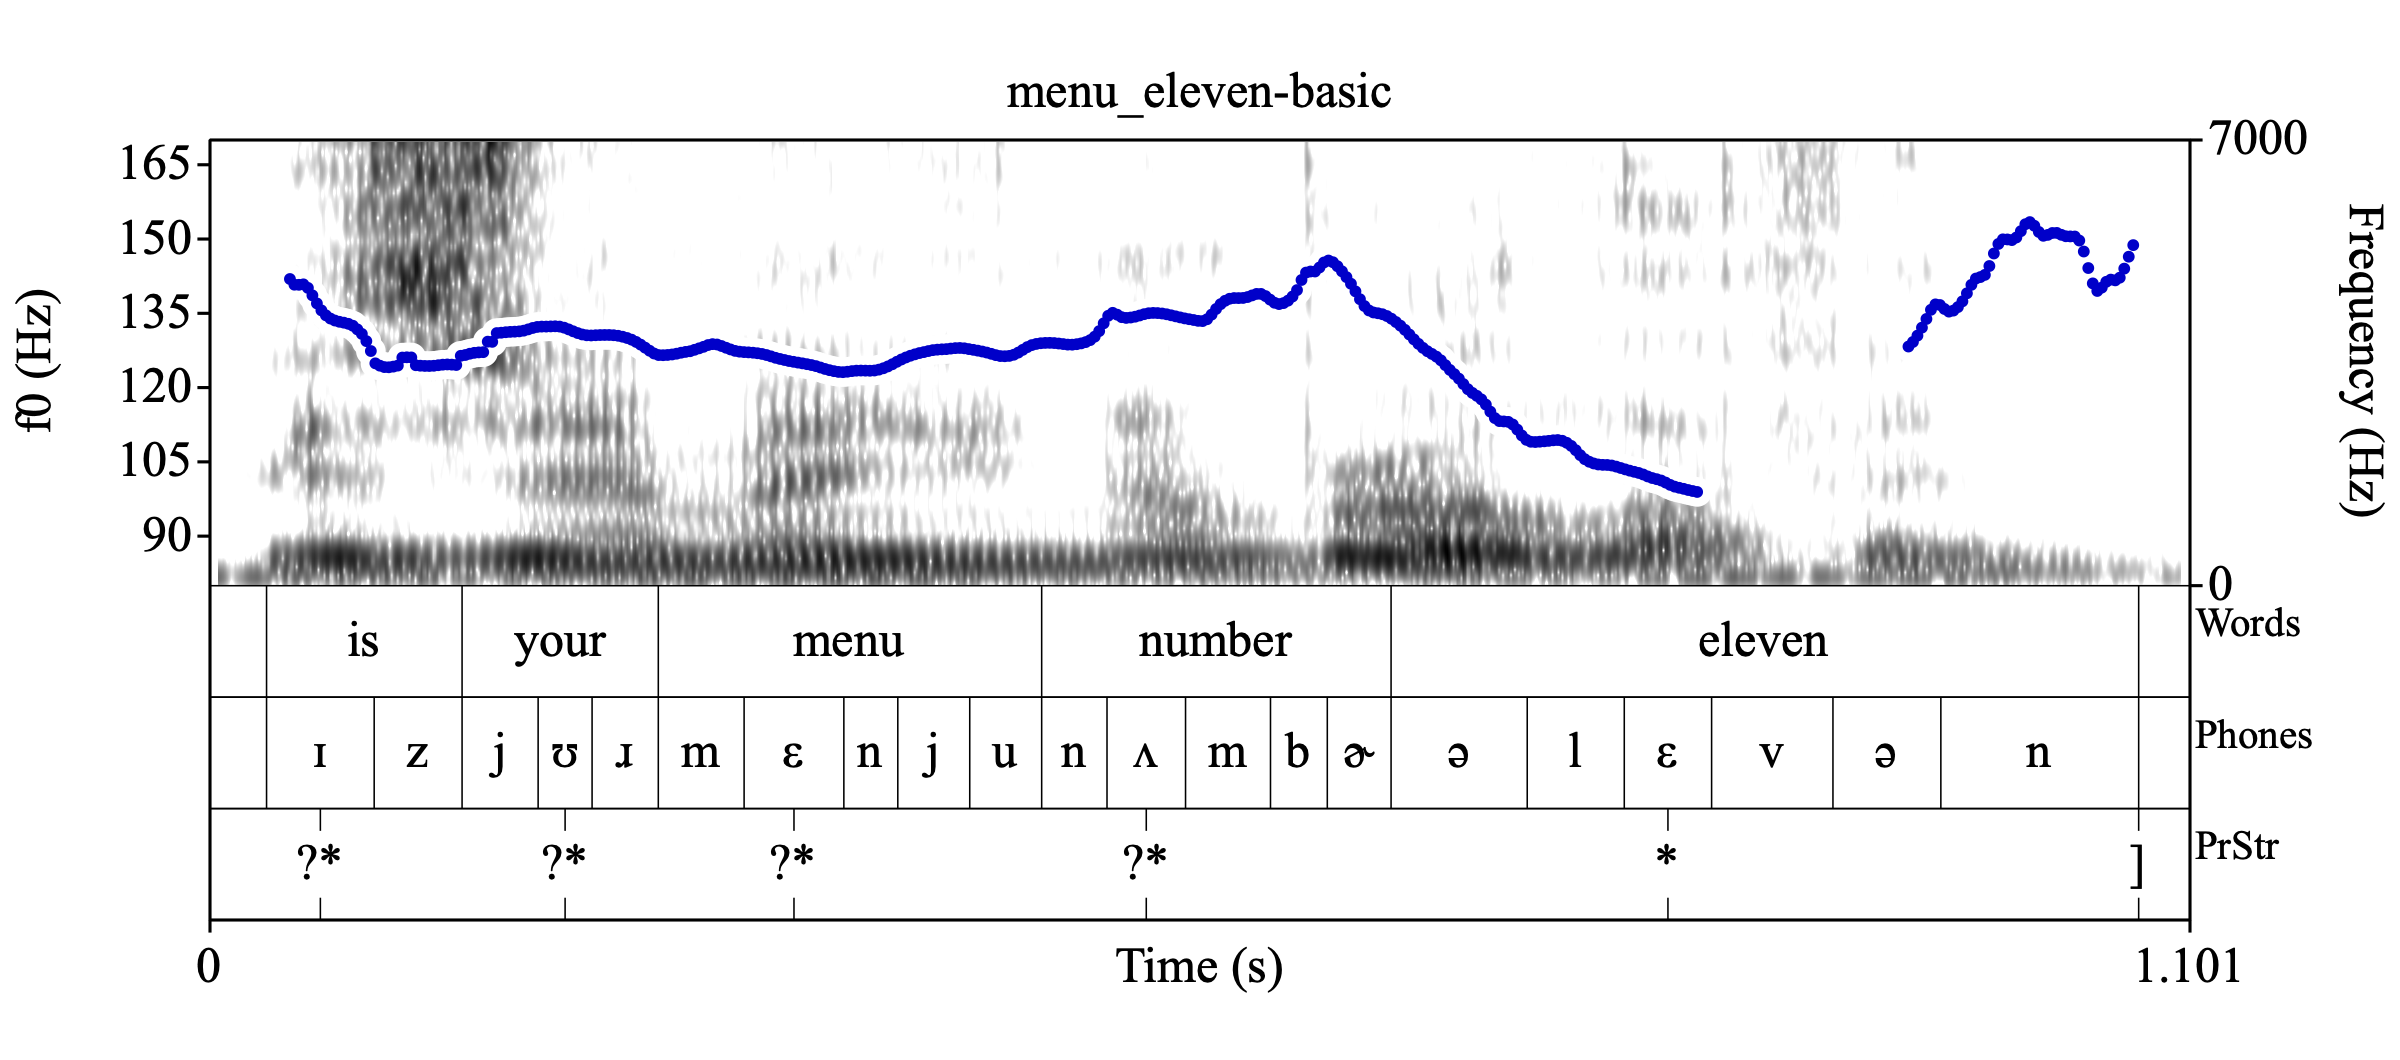
\includegraphics[width=.875\linewidth]{PrStr-menu_eleven-basic.png}
%
\caption{\texttt{menu\_eleven}: The labeller is uncertain as to whether any of the first four words are prominent or not.%
\label{fig:menu eleven PrStr uncertainty}%
\index{Annotated example, PrStr tier!menu\_eleven}
}
\end{figure}

Additional cases illustrating labeller uncertainty are provided in the Advanced PoLaR labels chapter.

Similar to uncertainty labels for prominence, a labeller can indicate uncertainty about the presence of a phrase boundary using the ‘\textlabel{?]}’ label. For example, in \texttt{librivox-zip1}, the labeller is uncertain of whether there is a phrase boundary between “\langtext{Librivox}” and “\langtext{recording}”:

\begin{figure}[H]
\centering
%
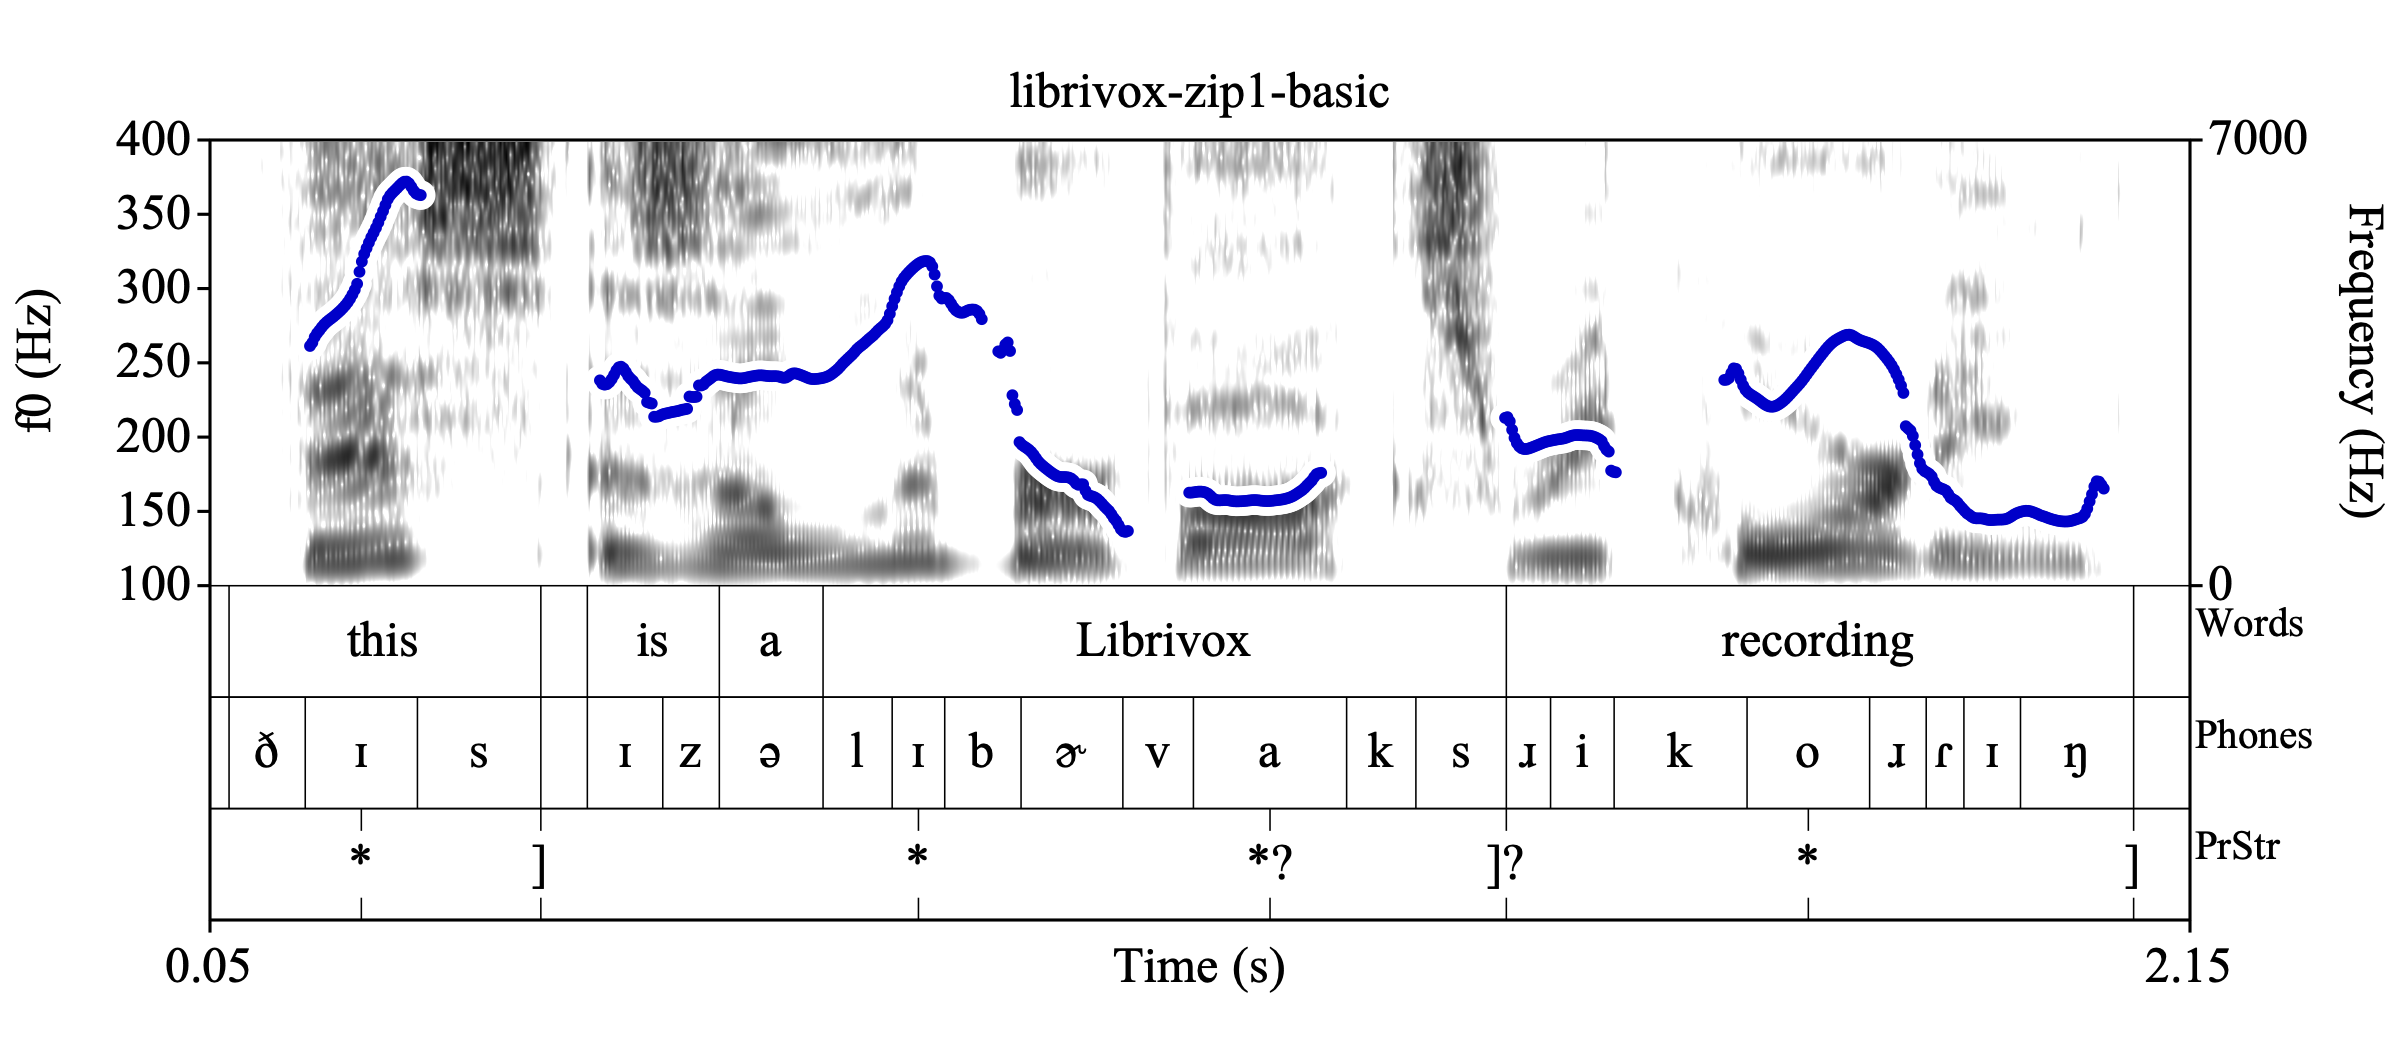
\includegraphics[width=.875\linewidth]{PrStr-librivox-zip1-basic.png}
%
\caption{\texttt{librivox-zip1}: The labeller is uncertain as to whether there is a prosodic phrase boundary between ‘Librivox’ and ‘recording’.%
\label{fig:librivox-zip1 PrStr uncertainty}%
\index{Annotated example, PrStr tier!librivox-zip1}
}
\end{figure}

(Note that there is also a \textlabel{?*} on the final syllable of “\langtext{Librivox}”.) Again, additional cases of labeller uncertainty are provided in chapter \ref{ch:advanced}.

Explicitly annotating uncertainty may be useful for future analysis of which cues local to \textlabel{*} and \textlabel{]} labels are reliably informative to a labeller regarding the presence of prominence and phrasing, and what sorts of acoustics lead to labeller uncertainty, as well as for studies of individual differences in cue interpretation. Additionally, an experienced labeller may have intuitions about why they are uncertain about the existence of prominence\slash phrasing; in such cases, the labeller is encouraged to annotate these intuitions on a “miscellaneous” tier.\footnote{This is because, though some cues to prominence and phrasing are annotated elsewhere (e.g., the Points and Ranges tiers), it can be helpful for future readers of labels if the labeller includes more explicit information about what led the labeller to be uncertain. (This may be especially helpful for coming to consensus labels, when multiple labellers PoLaR-annotate the same file.)}

\subsubsection{Examples of Basic Prosodic Structure labels}\label{sec:more-examples}

In this section you will find additional figures, showing audio examples labelled with PrStr labels. The name of each sound file is provided in the caption for each figure, and those sound files (and corresponding TextGrids) can be found at \url{https://www.polarlabels.com}. These figures show the words, the phones, and the PrStr labels. In some cases, MAE\_ToBI Tones labels\footnote{The alignment of the ToBI Tones tier labels follows \citealt{beckman-05} (p.25), where it is stated that pitch accent labels should be timed within the accented syllable, in such a way that it is nearest to the appropriate f0 minimum\slash maximum. Some laboratories prefer that pitch accent labels (on ToBI Tones tier) be time-aligned to occur within the stressed syllable’s nucleus (as was the guidance in earlier ToBI materials; e.g., \citealt{beckmanhirschberg94}).} are given alongside PrStr labels for comparison; but readers of these annotations do \uline{not} need to understand MAE\_ToBI to continue on with PoLaR.\footnote{Note that, by design, PrStr labels (on their own) encode less information than ToBI Tones labels.} The original TextGrid files used to produce these figures have additional annotation, with other PoLaR tiers.

\paragraph{Basic PrStr Examples 1 and 2: differences in edge tones}

The following examples share the same words and prominence locations but differ in how the speaker chooses to vary the f0 to mark the phrase edge tones. In PoLaR, these final boundaries would both be marked with the \textlabel{]} symbol and the acoustic distinction will be annotated in other tiers (e.g., in the Points Tier, as discussed in the next section, §\ref{sec:points}). For those familiar with ToBI labels, which we have included in these examples, note that the f0 contrast (falling to a low vs rising f0) and the prosodic function (disjuncture) labels are bundled together. 

\begin{figure}[H]
\centering
%
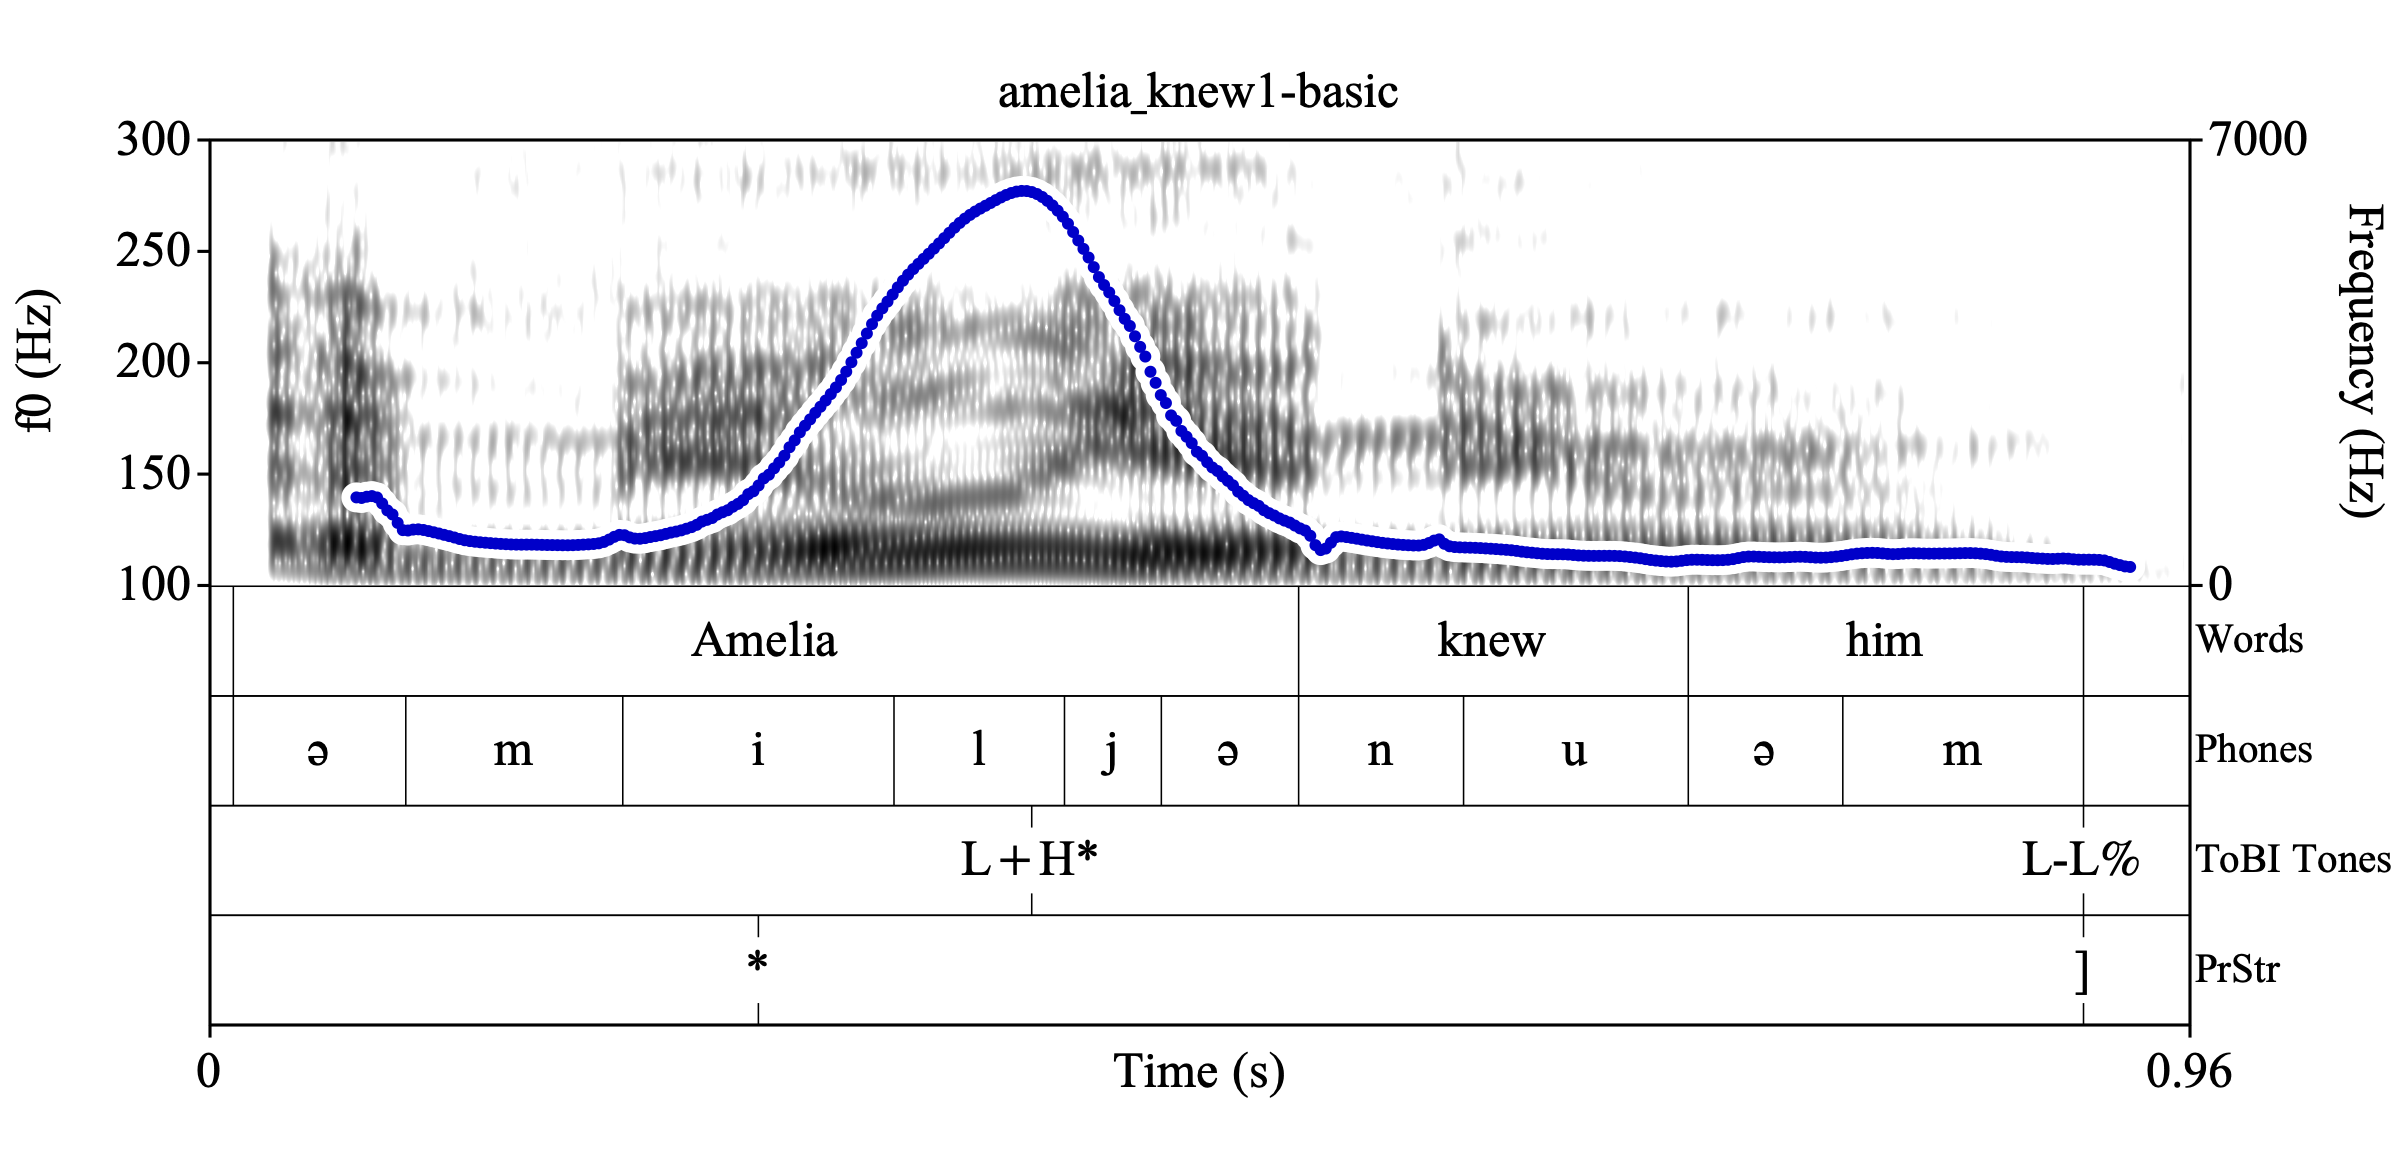
\includegraphics[width=.875\linewidth]{PrStr-amelia_knew1-basic.png}
%
\caption{\texttt{amelia-knew1}, with the PrStr tier annotated.%
\label{fig:amelia-knew1 PrStr}%
\index{Annotated example, PrStr tier (basic)!amelia-knew1}%
}
\end{figure}

\begin{figure}[H]
\centering
%
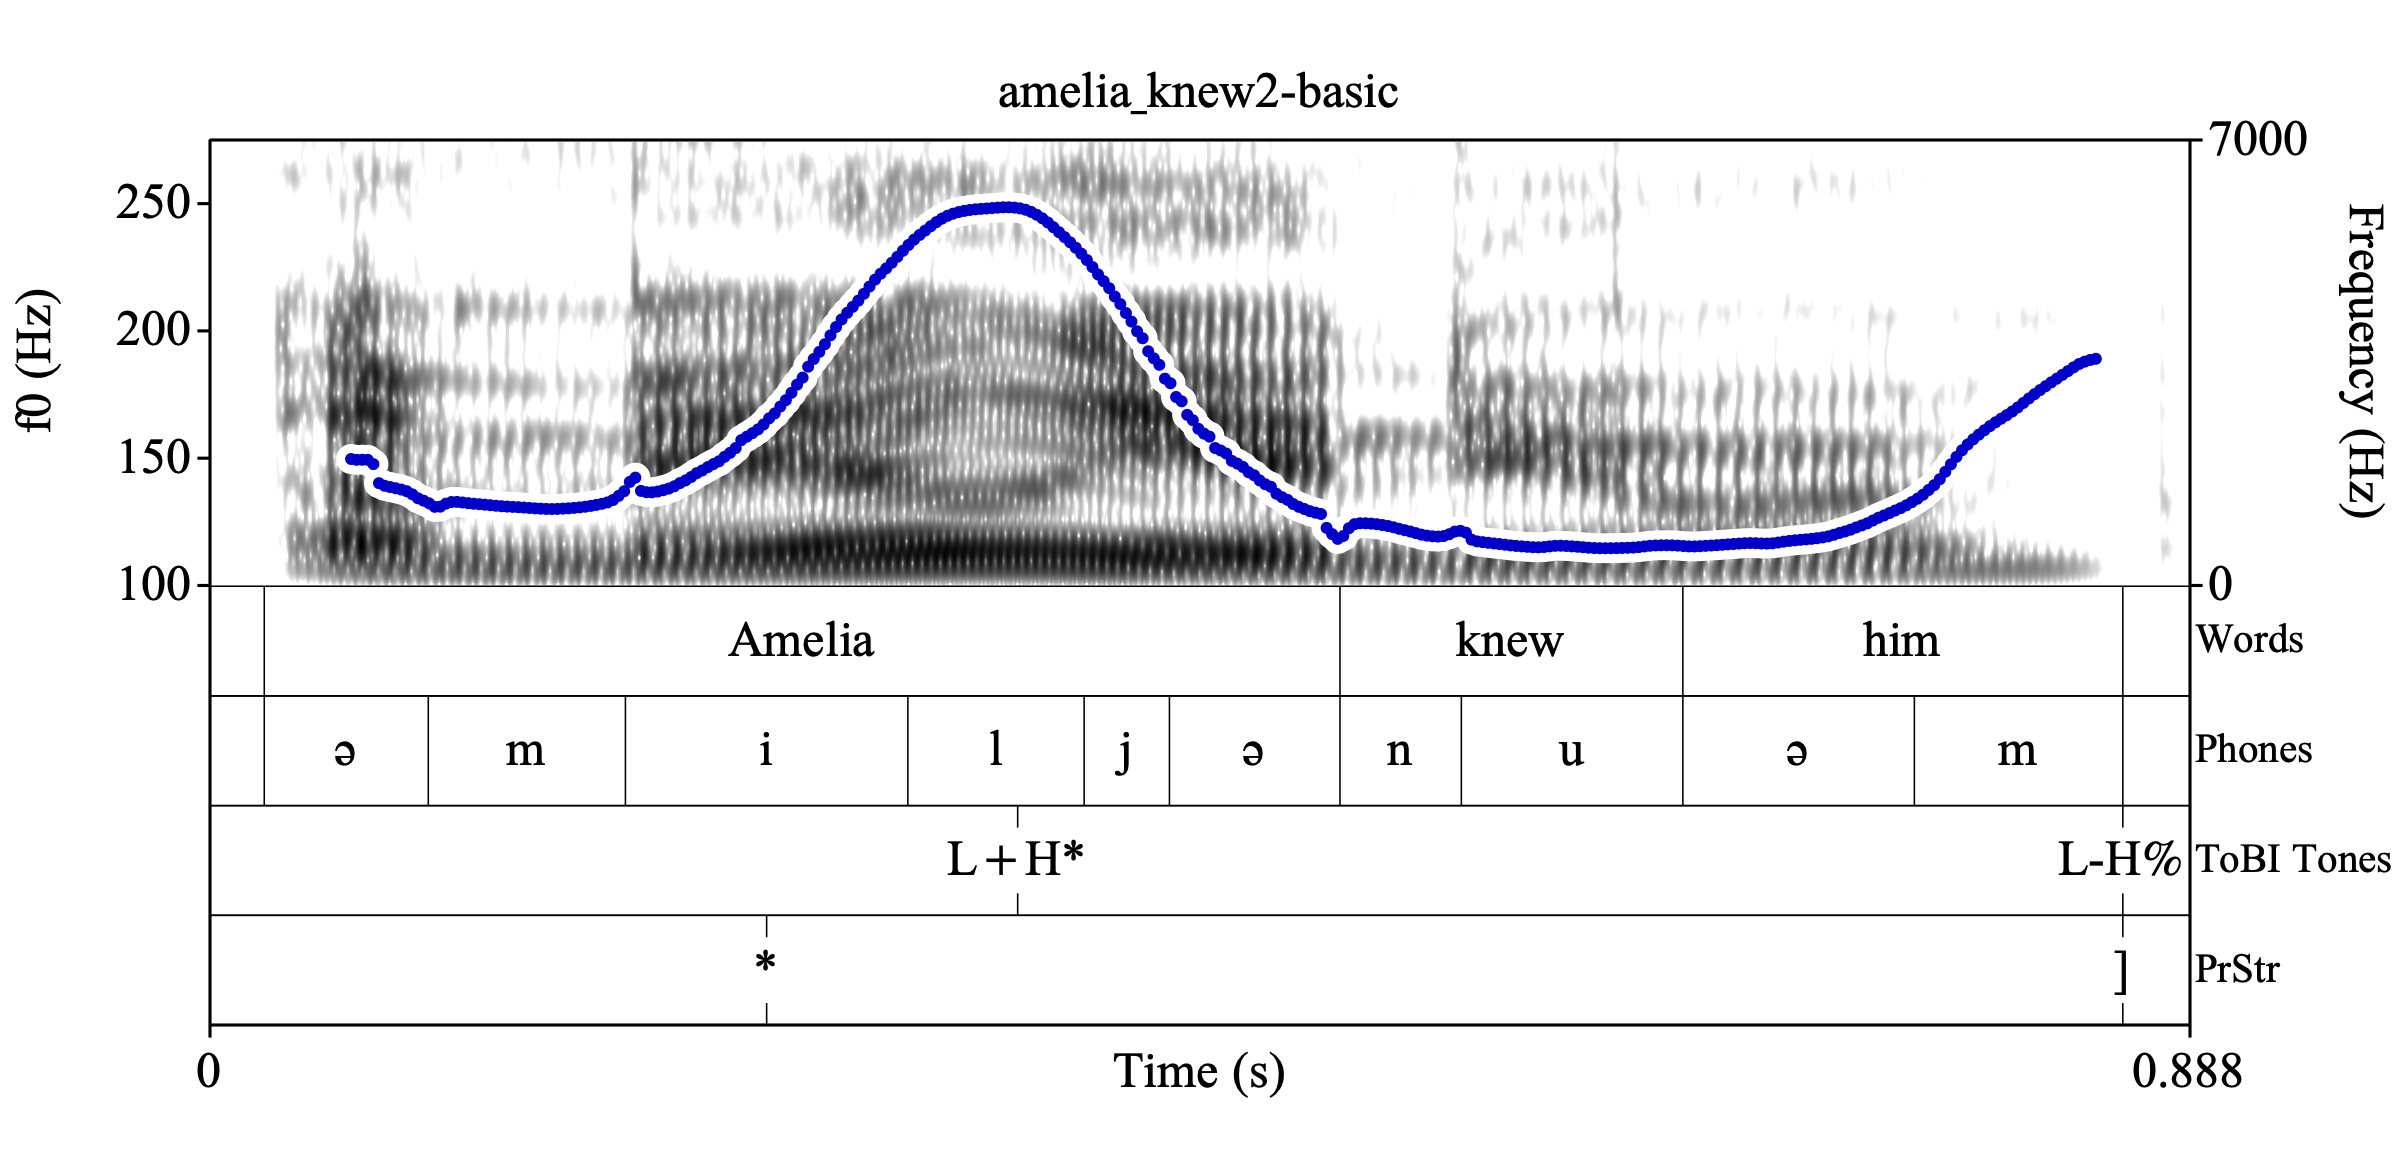
\includegraphics[width=.875\linewidth]{PrStr-amelia_knew2-basic.png}
%
\caption{\texttt{amelia-knew2}, with the PrStr tier annotated.%
\label{fig:amelia-knew2 PrStr}%
\index{Annotated example, PrStr tier (basic)!amelia-knew2}%
}
\end{figure}

\paragraph{Basic PrStr Examples  3 and 4: label locations}

Although changes in f0 are often very visually salient cues to prosodic structure, particularly prominences, PoLaR PrStr labels are situated with respect to the word string. Here the \textlabel{*} label is placed in the center of the transcribed [ɪ] vowel rather than at the f0 peak. The \textlabel{]} label is at the end of the final word in the phrase. 


\begin{figure}[H]
\centering
%
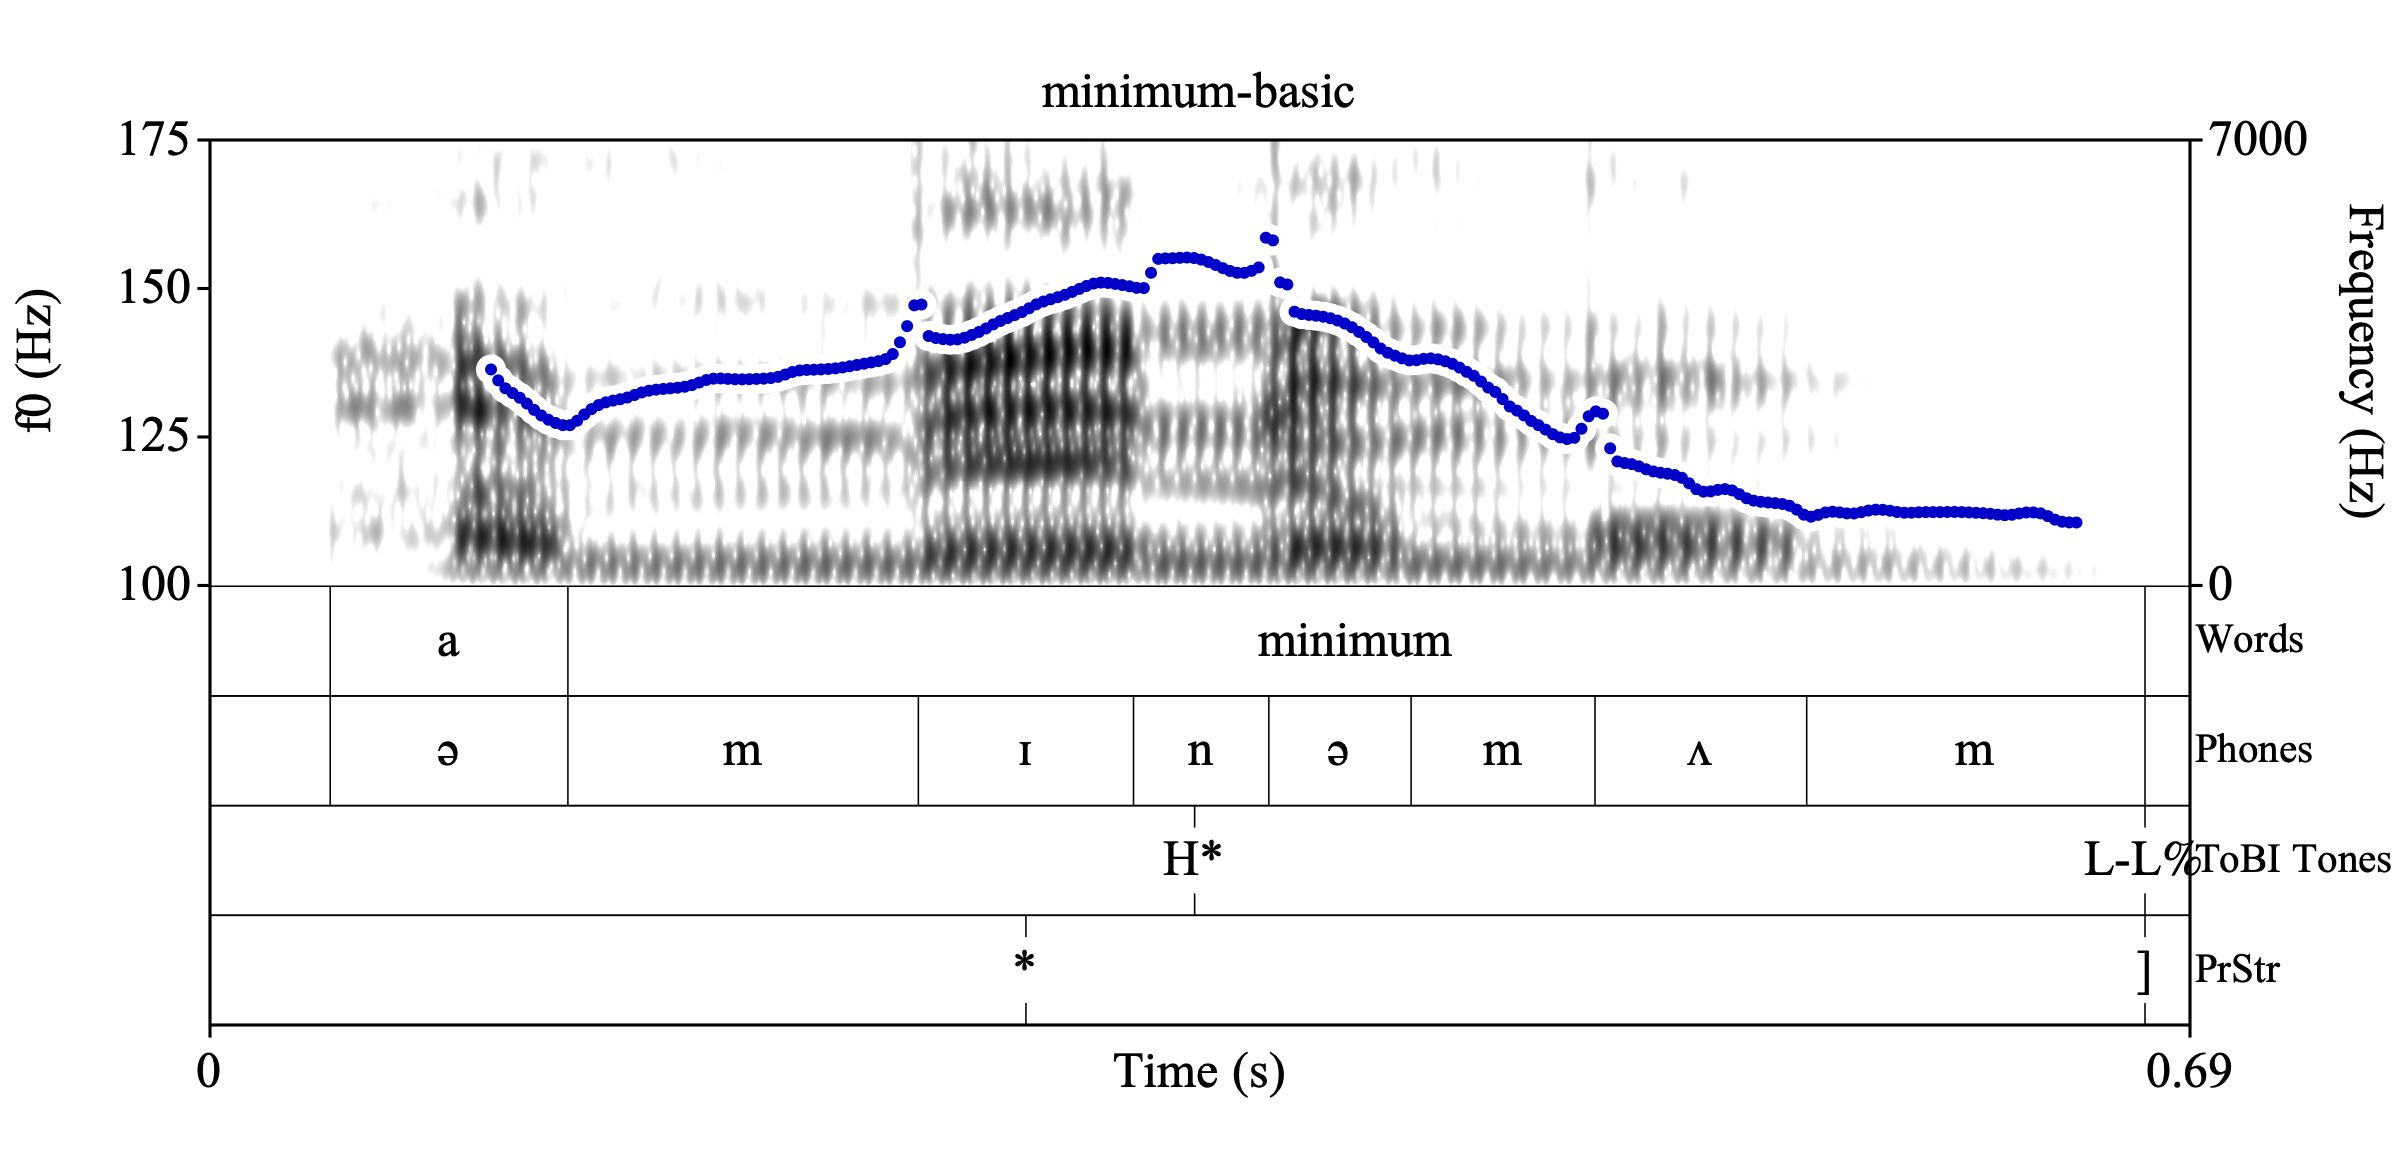
\includegraphics[width=.875\linewidth]{PrStr-minimum-basic.png}
%
\caption{\texttt{minimum}, with the PrStr tier annotated.%
\label{fig:minimum PrStr}%
\index{Annotated example, PrStr tier (basic)!minimum}%
}
\end{figure}

Similarly, the \textlabel{*} label is placed in the middle of the transcribed [i] rather than in the high f0 that cues the prominence. 

\begin{figure}[H]
\centering
%
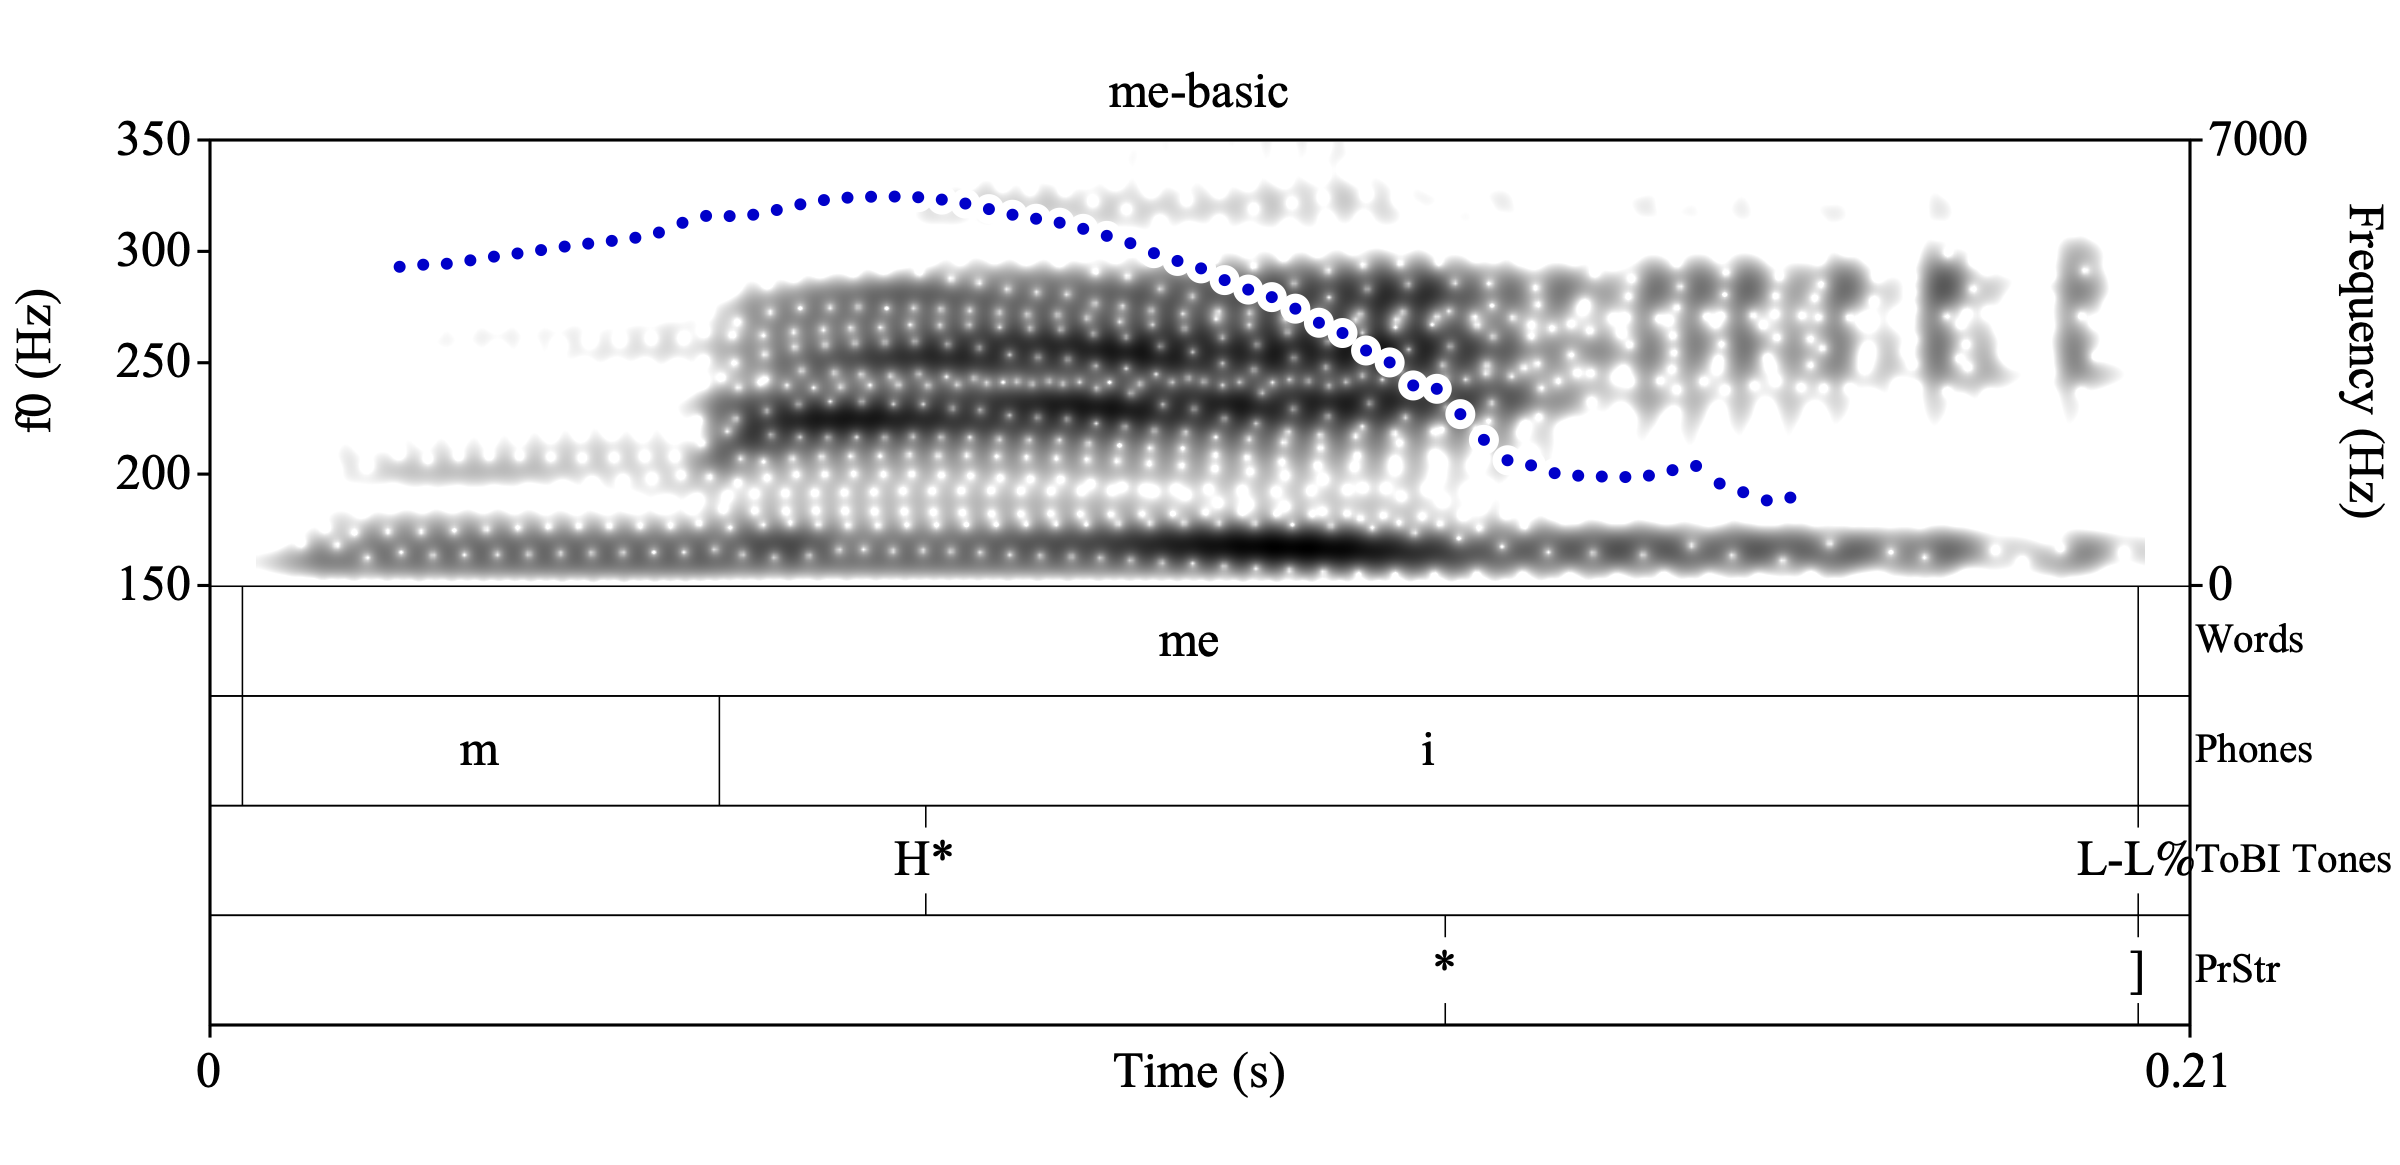
\includegraphics[width=.875\linewidth]{PrStr-me-basic.png}
%
\caption{\texttt{me}, with the PrStr tier annotated.%
\label{fig:me PrStr}%
\index{Annotated example, PrStr tier (basic)!me}%
}
\end{figure}

\paragraph{Basic PrStr Examples 5, 6, 7: multiple phrases and prominences in the same utterance}

Even short utterances can have more than one phrase. In general every phrase will have one or more prominences.  Labelers should use their intuitions as well as visual cues in the speech display to determine which words bear prominence or are in the same group.

\begin{figure}[H]
\centering
%
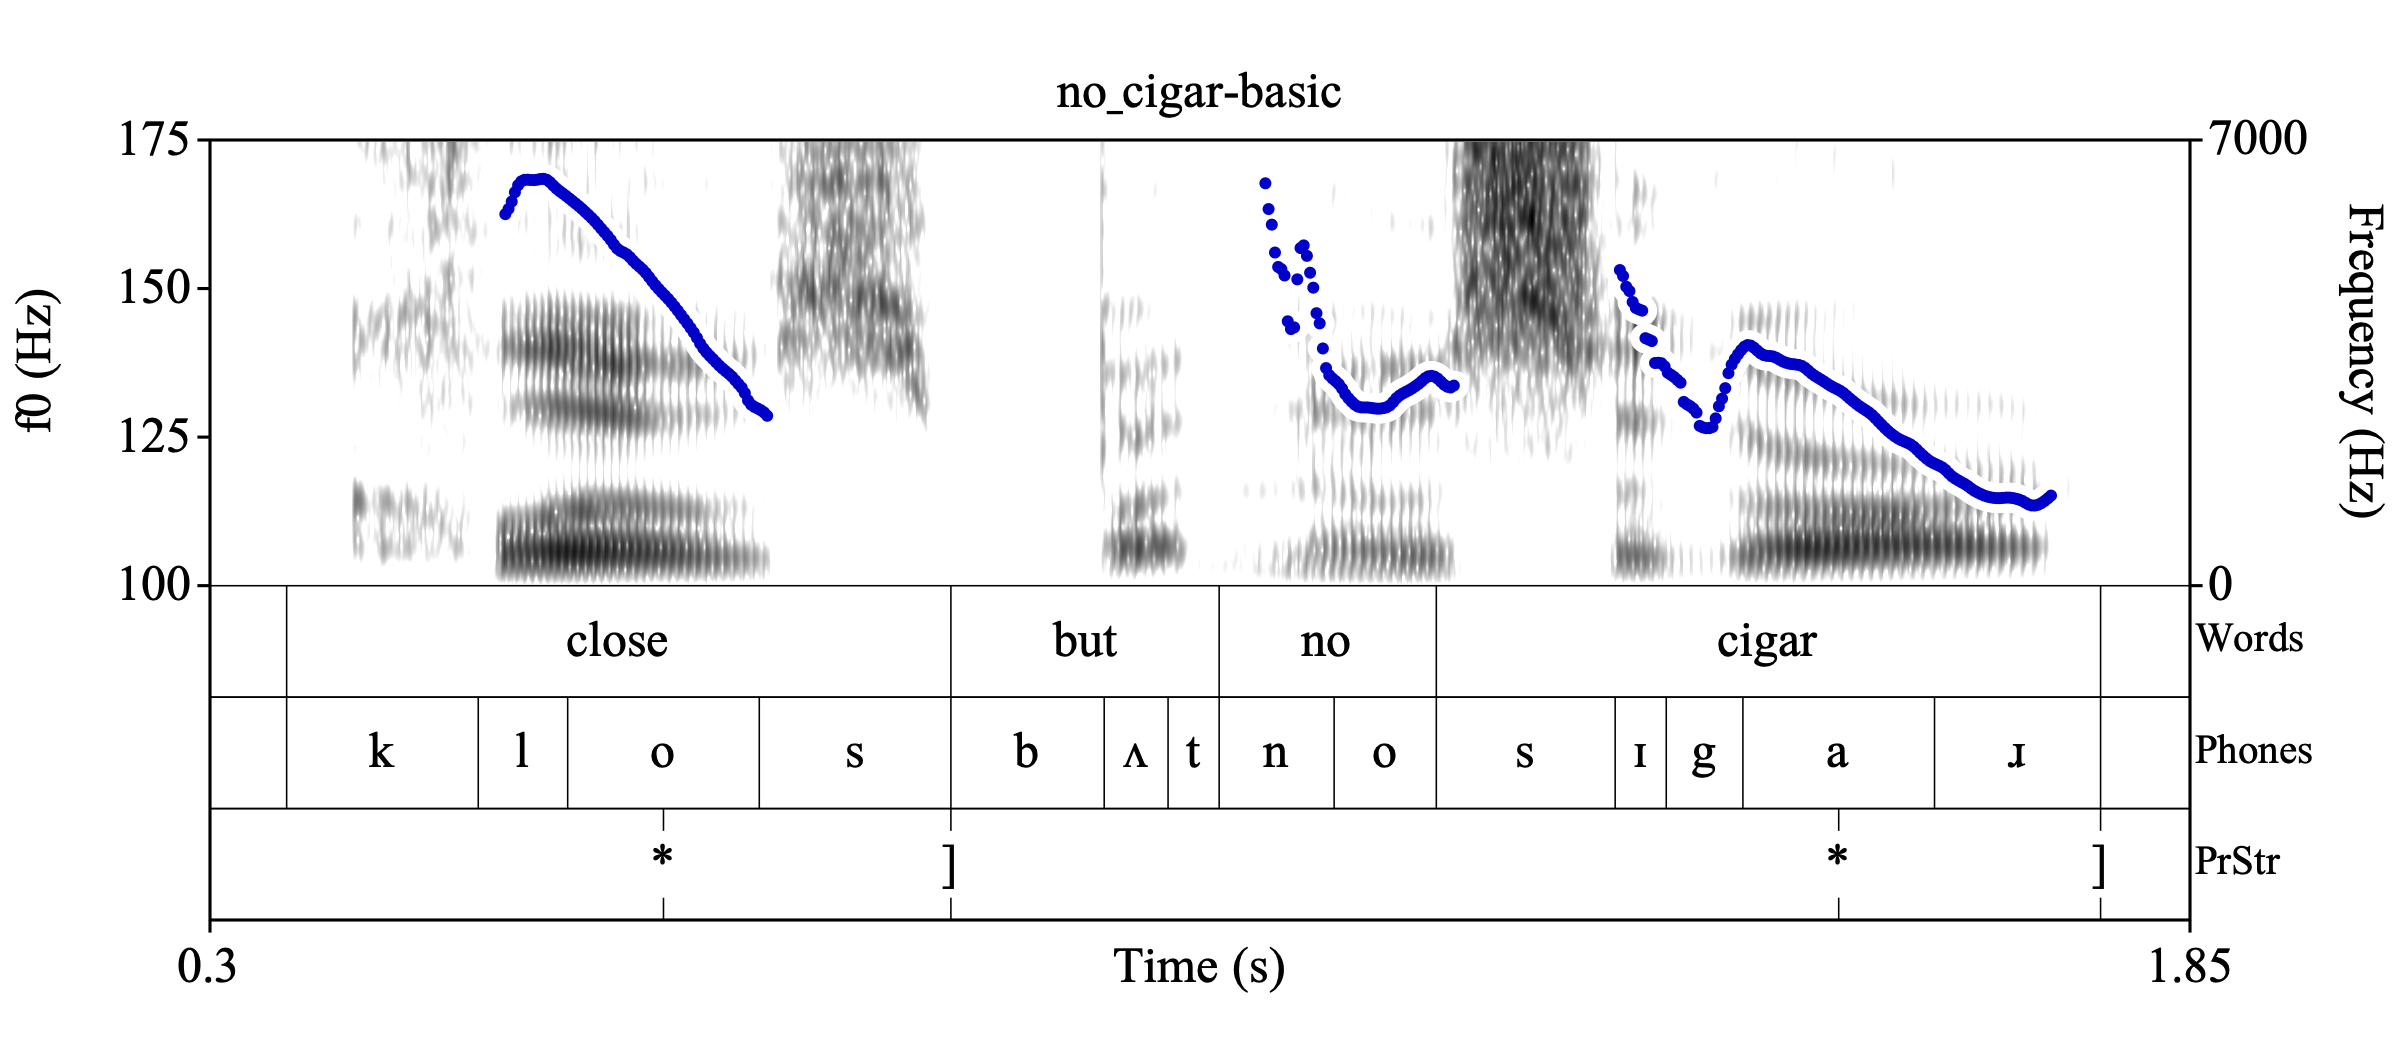
\includegraphics[width=.875\linewidth]{PrStr-no_cigar-basic.png}
%
\caption{\texttt{no\_cigar}, with the PrStr tier annotated.%
\label{fig:no_cigar PrStr}%
\index{Annotated example, PrStr tier (basic)!no\_cigar}%
}
\end{figure}

\begin{figure}[H]
\centering
%
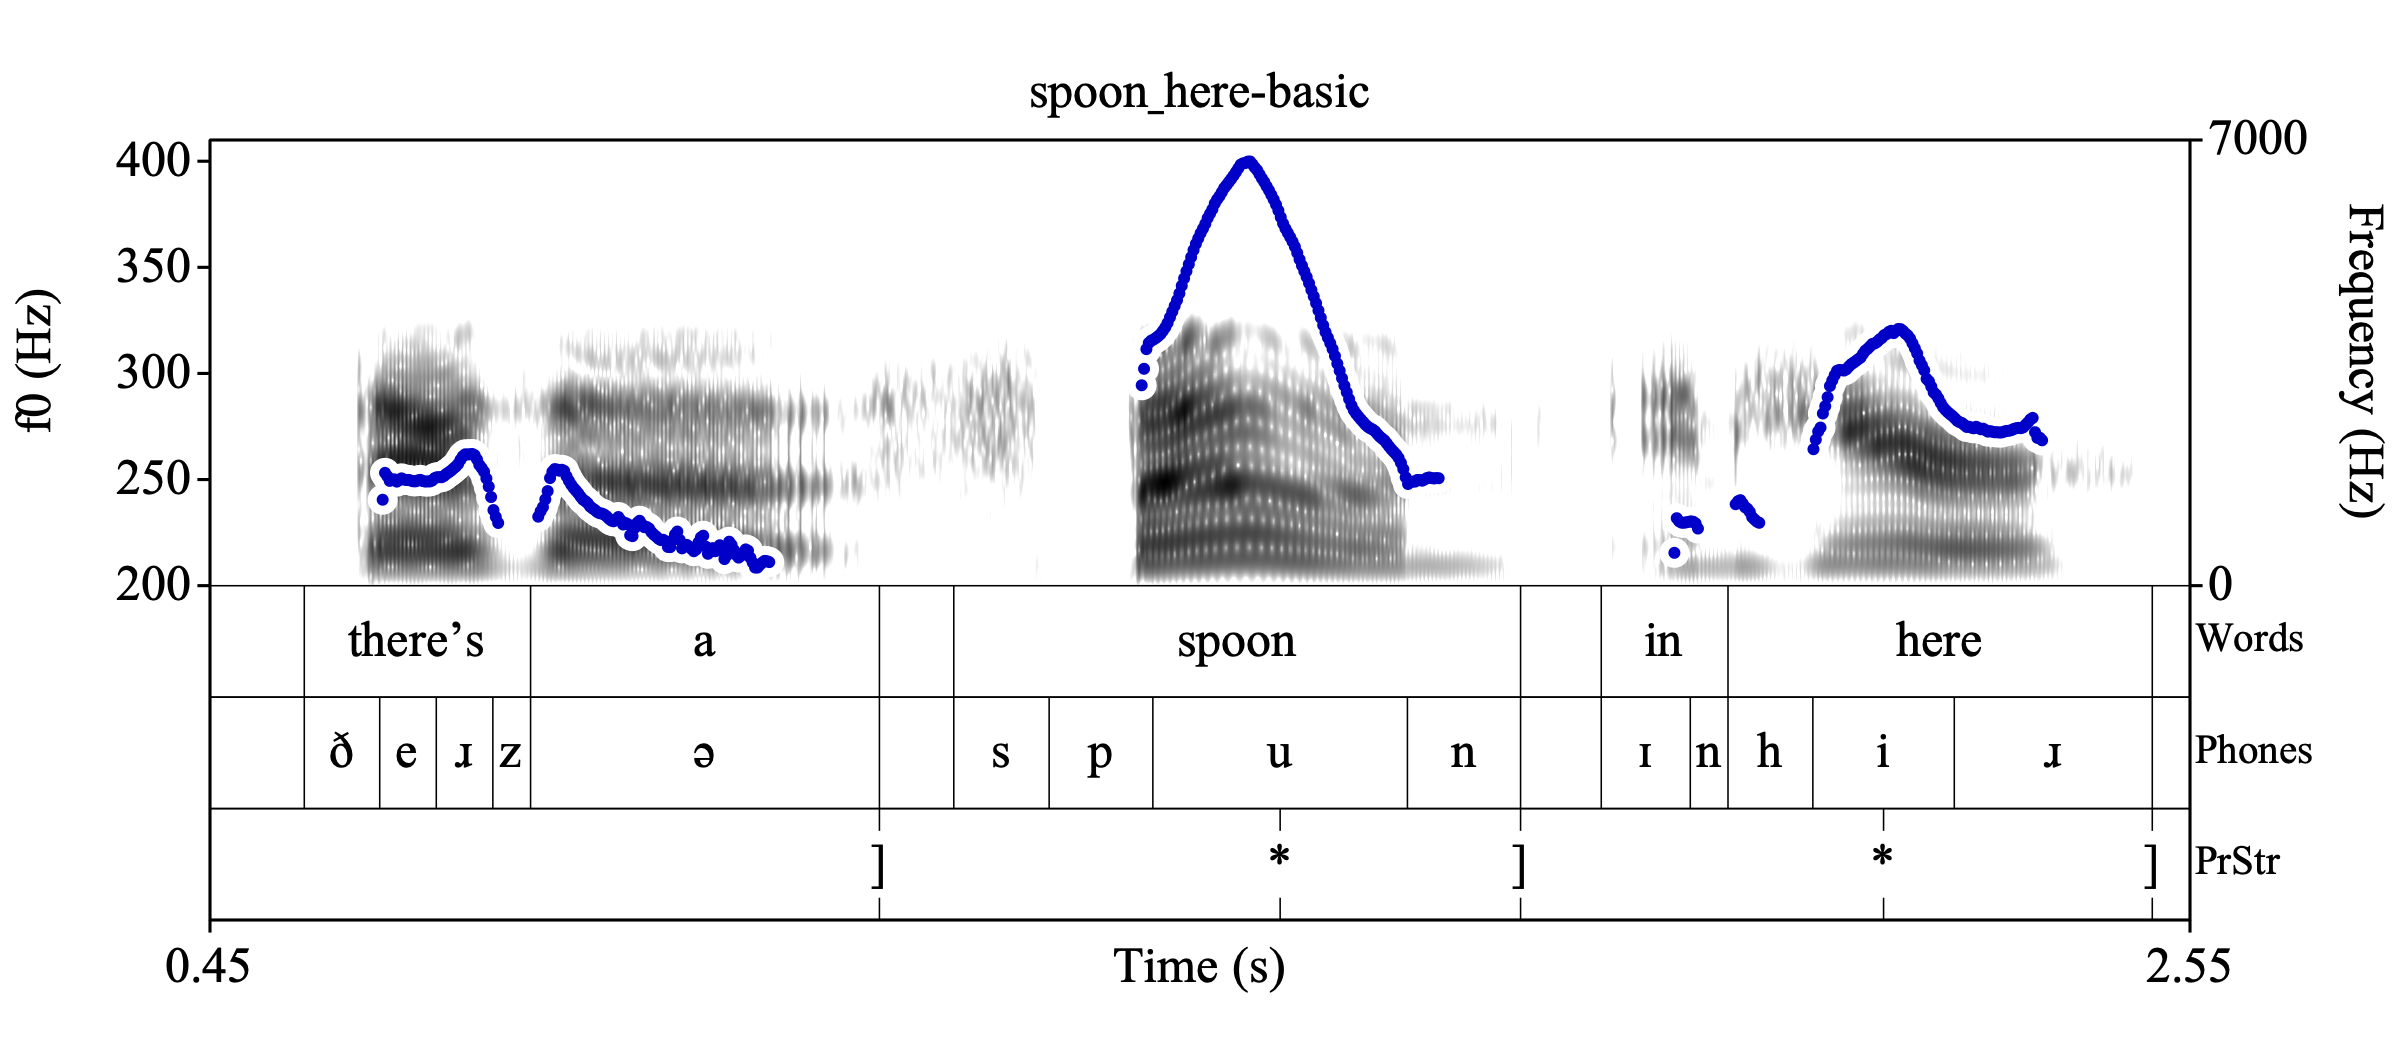
\includegraphics[width=.875\linewidth]{PrStr-spoon_here-basic.png}
%
\caption{\texttt{spoon\_here}, with the PrStr tier annotated.%
\label{fig:spoon_here PrStr}%
\index{Annotated example, PrStr tier (basic)!spoon\_here}%
}
\end{figure}

\begin{figure}[H]
\centering
%
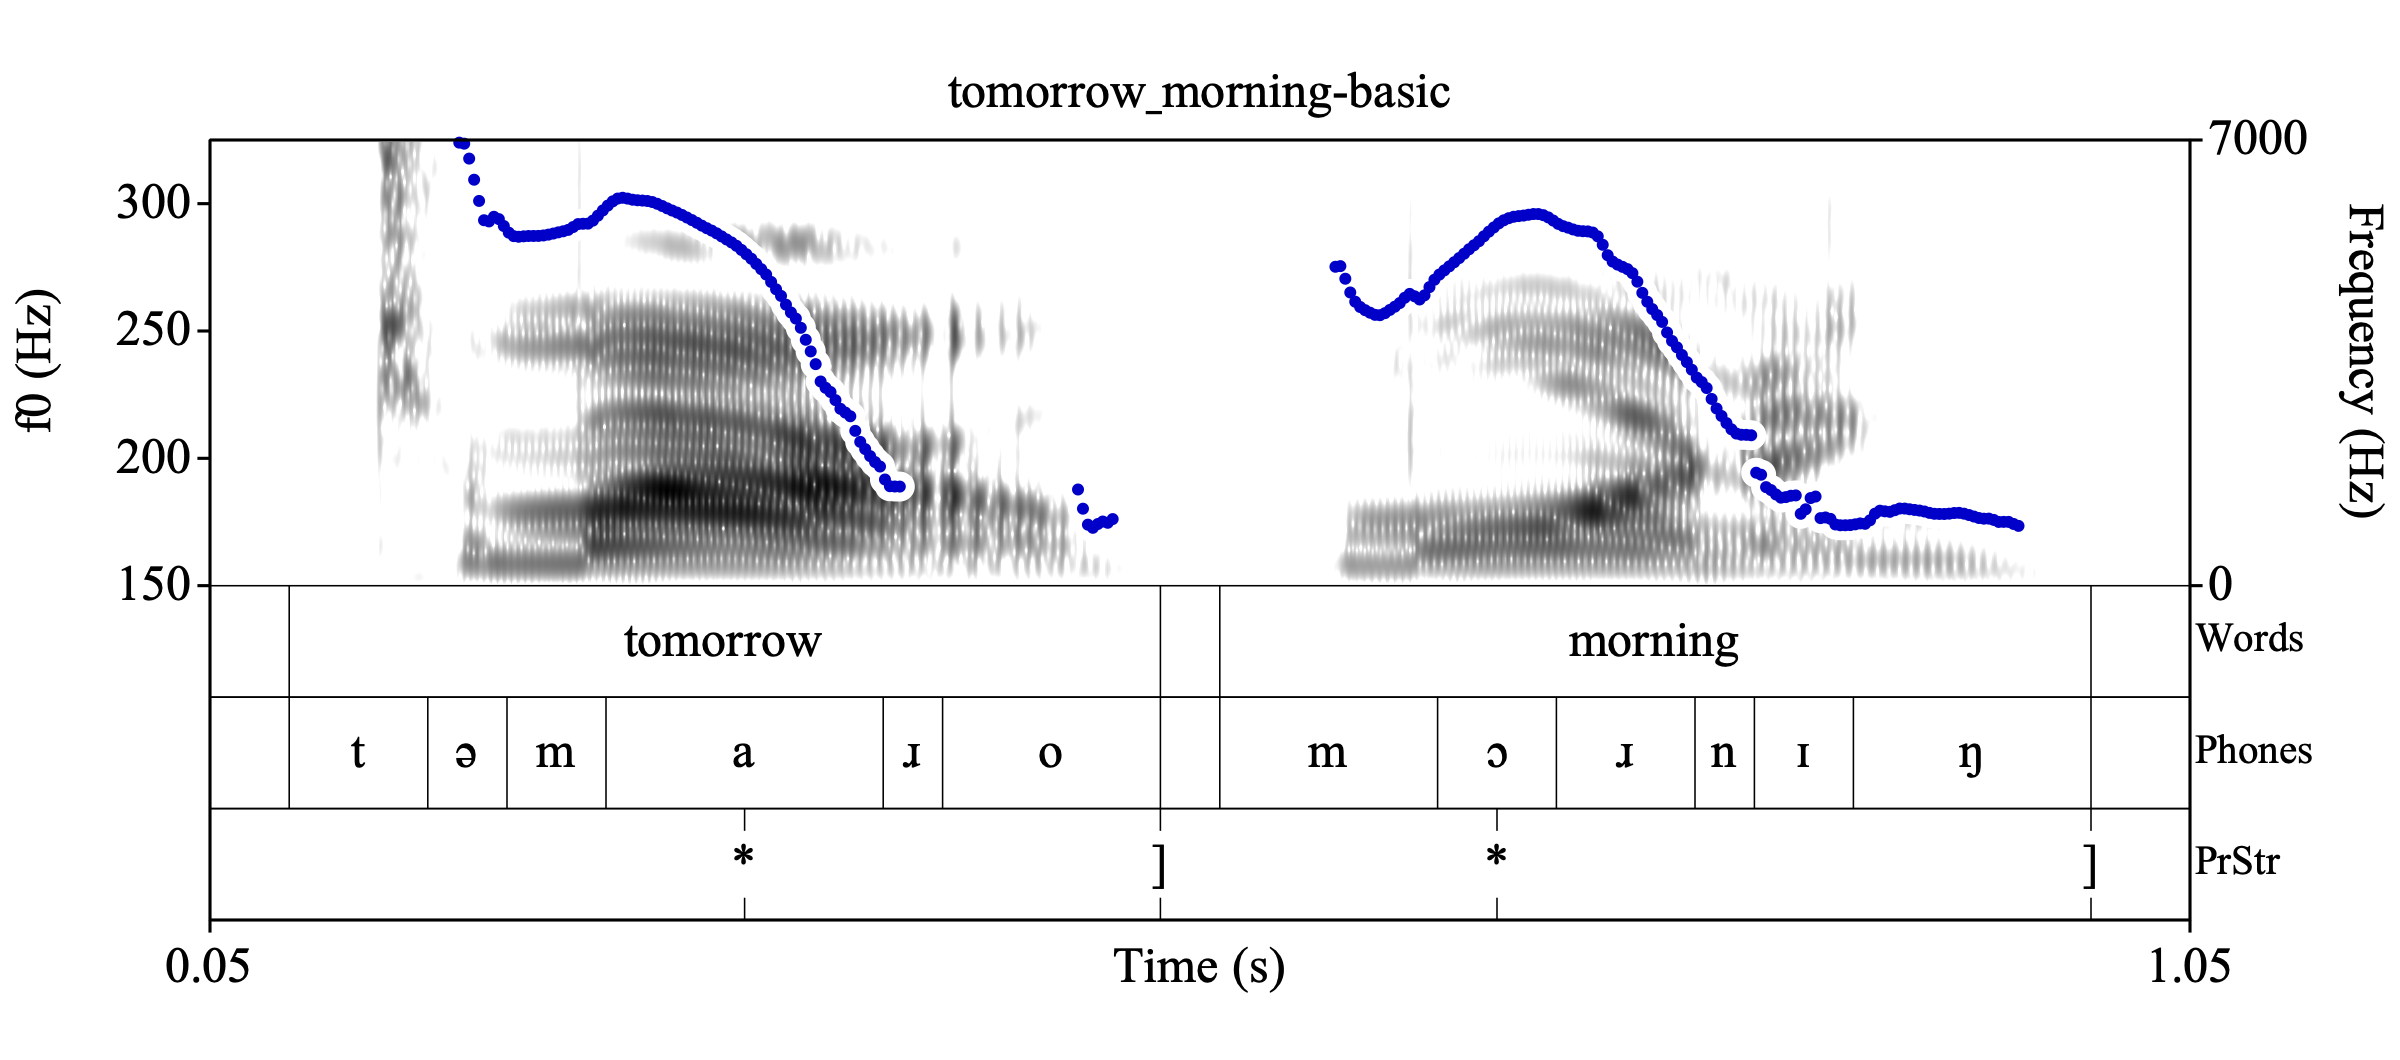
\includegraphics[width=.875\linewidth]{PrStr-tomorrow_morning-basic.png}
%
\caption{\texttt{tomorrow\_morning}, with the PrStr tier annotated.%
\label{fig:tomorrow_morning PrStr}%
\index{Annotated example, PrStr tier (basic)!tomorrow\_morning}%
}
\end{figure}

\paragraph{Basic PrStr Examples 8 and 9: F0 failure to fall}
As a cautionary note to labelers not to rely solely on the visual f0 displays (even when they are relatively accurate): not all prominences can be identified with notable rise-fall peaks. The following examples show that prominences on a series of words might be cued with a steady high f0 that doesn’t fall in between. 

\begin{figure}[H]
\centering
%
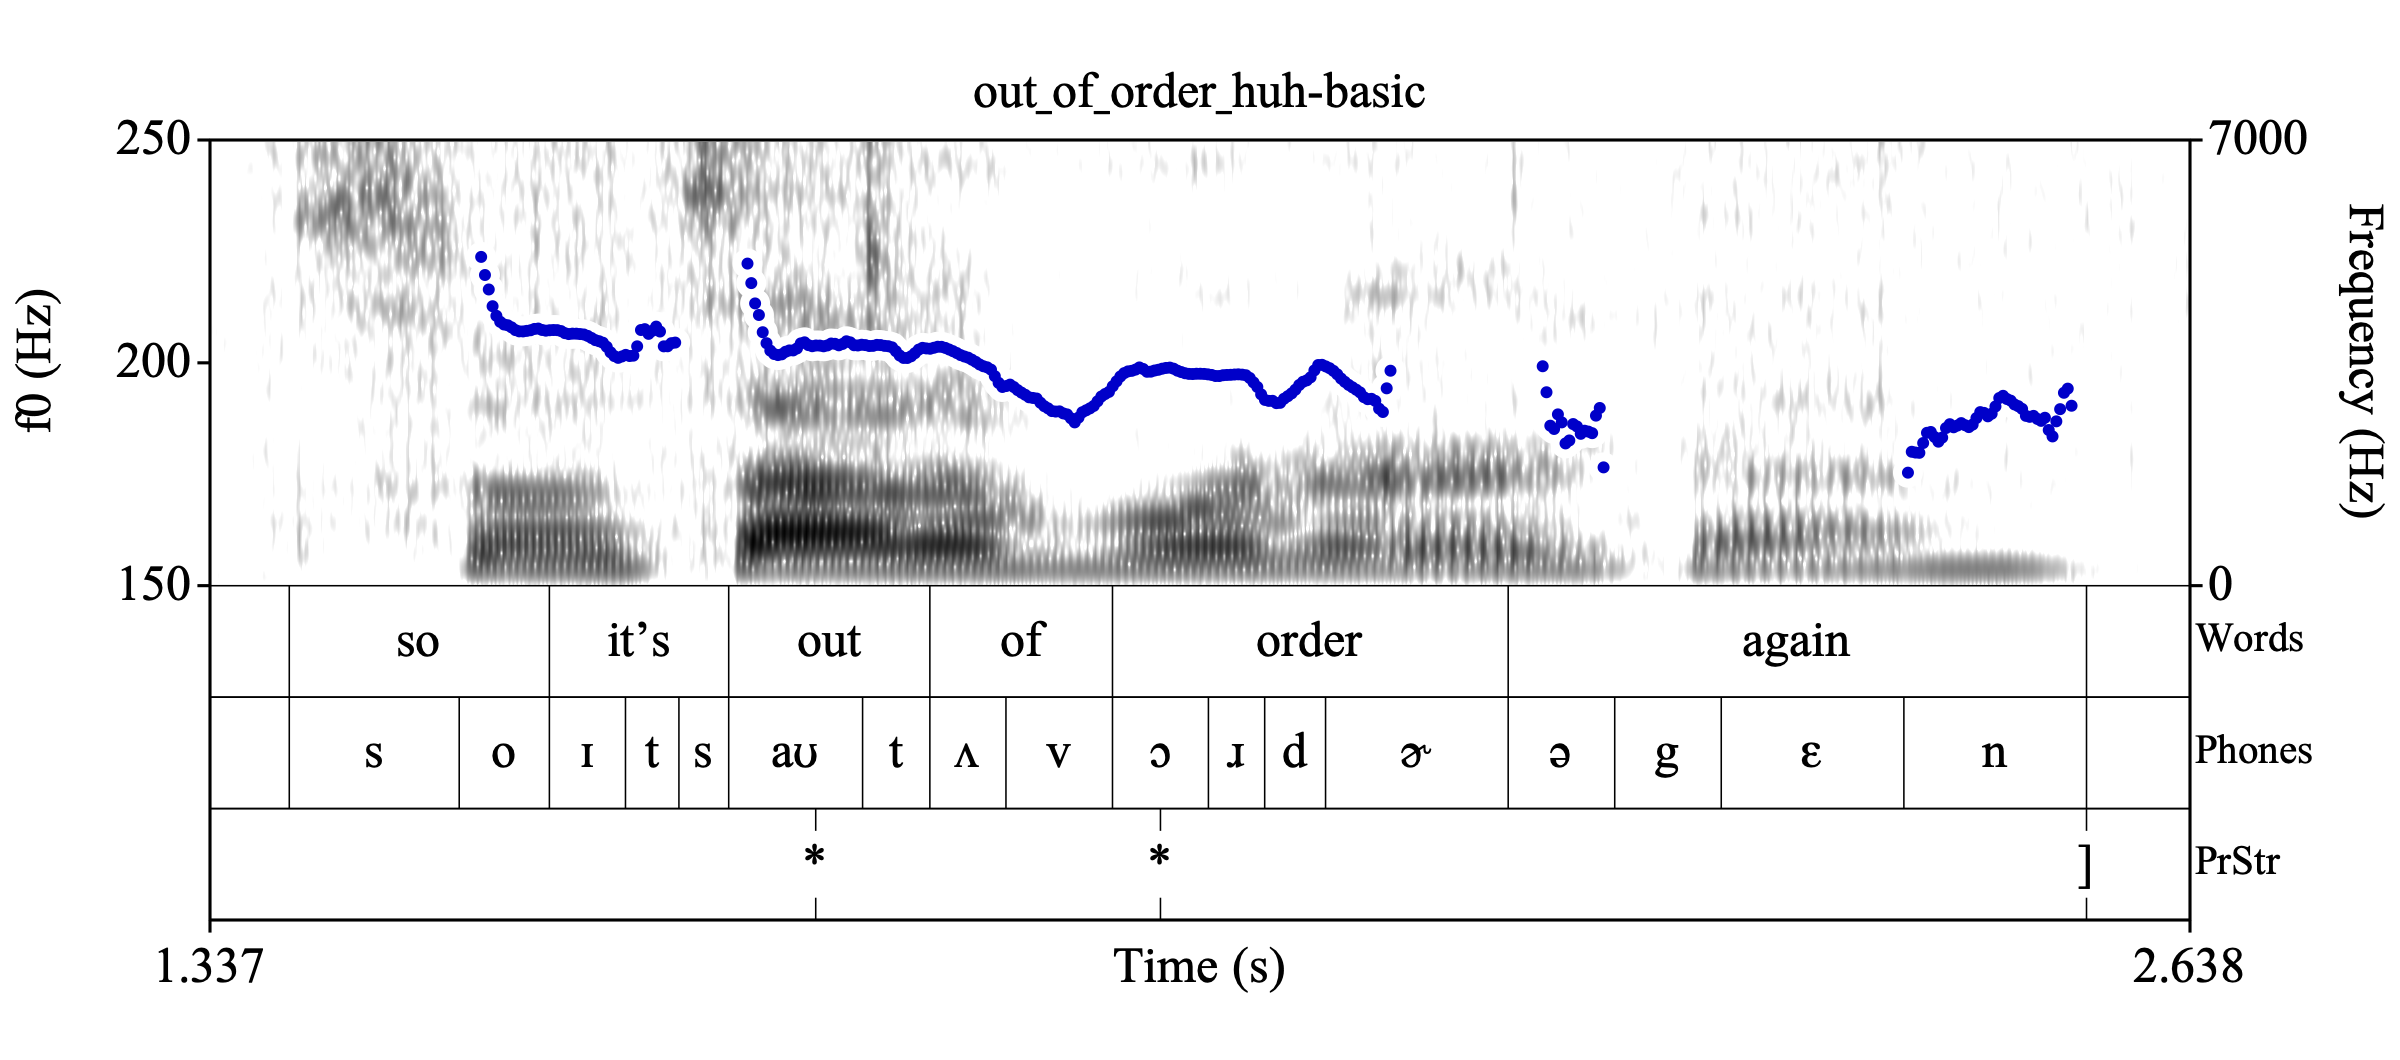
\includegraphics[width=.875\linewidth]{PrStr-out_of_order_huh-basic.png}
%
\caption{\texttt{out\_of\_order\_huh}, with the PrStr tier annotated.%
\label{fig:out_of_order_huh PrStr}%
\index{Annotated example, PrStr tier (basic)!out\_of\_order\_huh}%
}
\end{figure}

\begin{figure}[H]
\centering
%
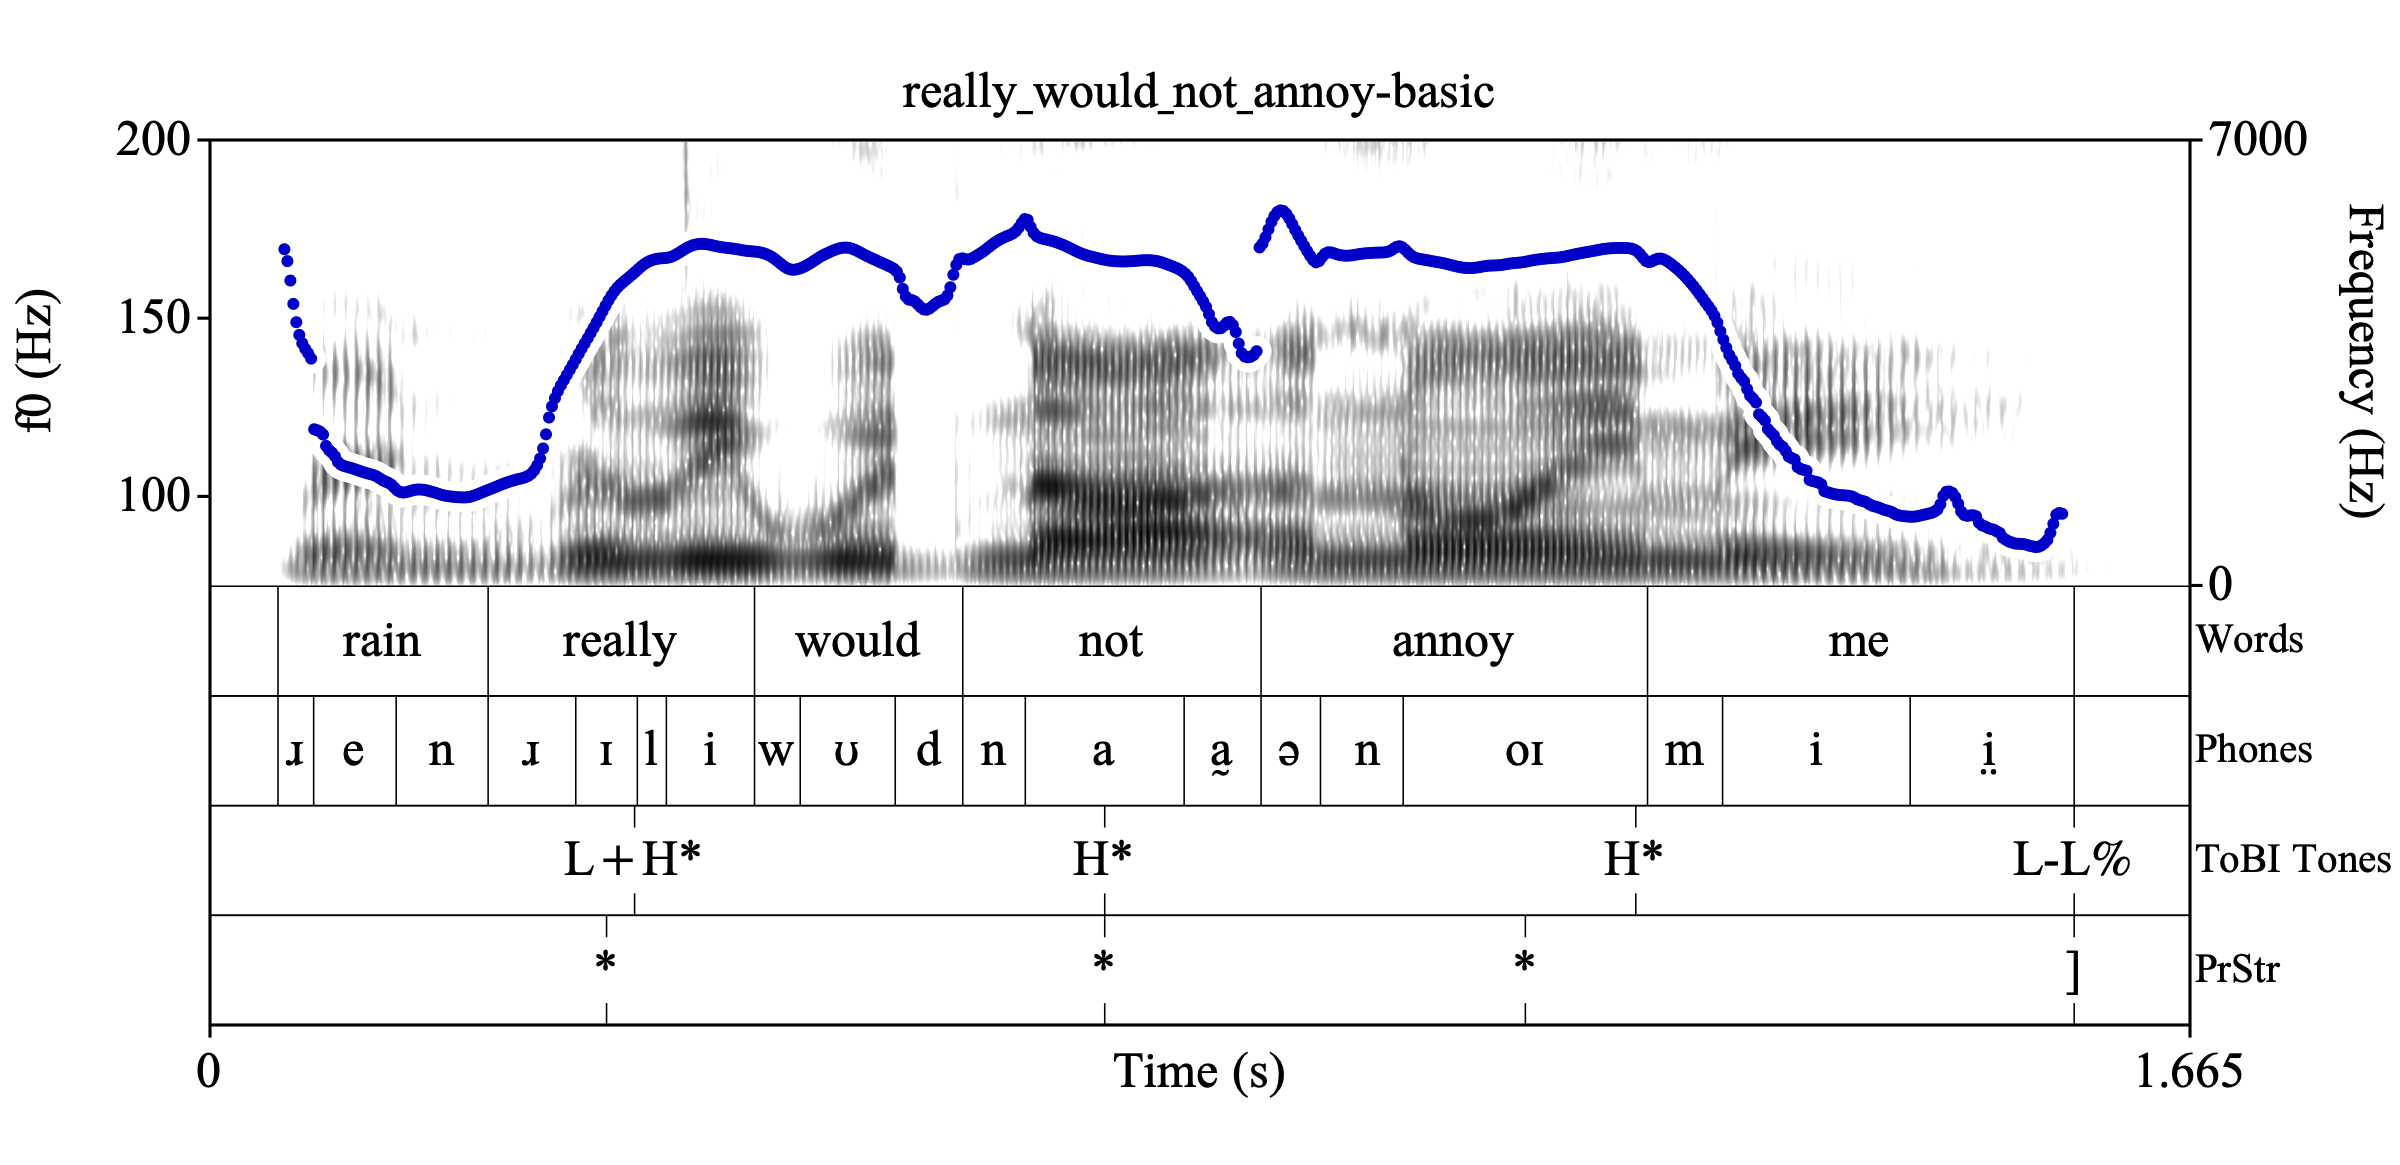
\includegraphics[width=.875\linewidth]{PrStr-really_would_not_annoy-basic.png}
%
\caption{\texttt{really\_would\_not\_annoy}, with the PrStr tier annotated.%
\label{fig:really_would_not_annoy PrStr}%
\index{Annotated example, PrStr tier (basic)!really\_would\_not\_annoy}%
}
\end{figure}


\subsubsection{PrStr labels summary}\label{sec:prstr-labels-summary}

The four PrStr Basic labels are named in Table \ref{PrStr basic labels}.

\begin{longtable}{clp{.525\linewidth}} \toprule \textbf{Label} & \textbf{Phonological Object} & \textbf{Label is time-aligned with \_\_\_\_\_}\tabularnewline
\midrule \endhead
\textlabel{*} & Prominence & A syllable that has intonational prominence \tabularnewline
\textlabel{?*} & Possible Prominence & A syllable that might have intonational prominence \tabularnewline
\textlabel{]} & Phrase’s Right Edge & The right edge of the final word of a phrase \tabularnewline
\textlabel{?]} & Possible Phrase’s Right Edge & What might be the right edge of the final word of a phrase \tabularnewline
\bottomrule 
\caption{The Basic labels for the Prosodic Structure tier (for English).%
\label{PrStr basic labels}%
}
\end{longtable}

\subsection{Points Tier}\label{sec:points}

With the Points Tier, we will focus on the changes in pitch, as observed through changes in fundamental frequency (f0). When discussing the pitch changes in an intonational contour, some approaches aim to define them as a sequence of phonological objects (e.g., a low pitch accent followed by a steady rise to a high boundary tone). However, such phonological objects are not directly observed in the acoustics, but rather are signalled with a variety of cues (e.g., pitch, duration, intensity, voice quality, etc.) – the primary purpose of the PoLaR Points tier is to identify the fundamental shape of the intonational contour.

\begin{infobox}[frametitle=\textbf{A NOTE ON TERMINOLOGY}]
Recall that f0 and pitch are different: f0 values can be measured directly from the speech signal, while pitch values are psycho-perceptual. Parallel to this, f0 contours track changes in f0 values, while intonational contours refer to abstract changes in pitch. Return to section \ref{sec:terminology} in Chapter \ref{ch:background} for more detailed discussion.\label{terminology f0 pitch}
\end{infobox}

PoLaR allows two levels of annotation detail on the Points Tier: the default (‘\textlabel{0}’) label is described in this chapter. (Advanced labels for associating the pitch turning points on the Points tier with the prosodic events on the PrStr tier, are described in Chapter \ref{ch:advanced}.)

Regardless of whether a labeller is using Basic or Advanced labels, the Points Tier is used to capture those significant turning points in a point-in-time tier. The goal (guidance below) is to annotate only and all of the f0 locations that are perceptually salient. (We will describe some f0 movements that are \emph{not} perceptually salient, later in this section.) Consider the f0 contour in the following example:

\begin{figure}[H]
\centering
%
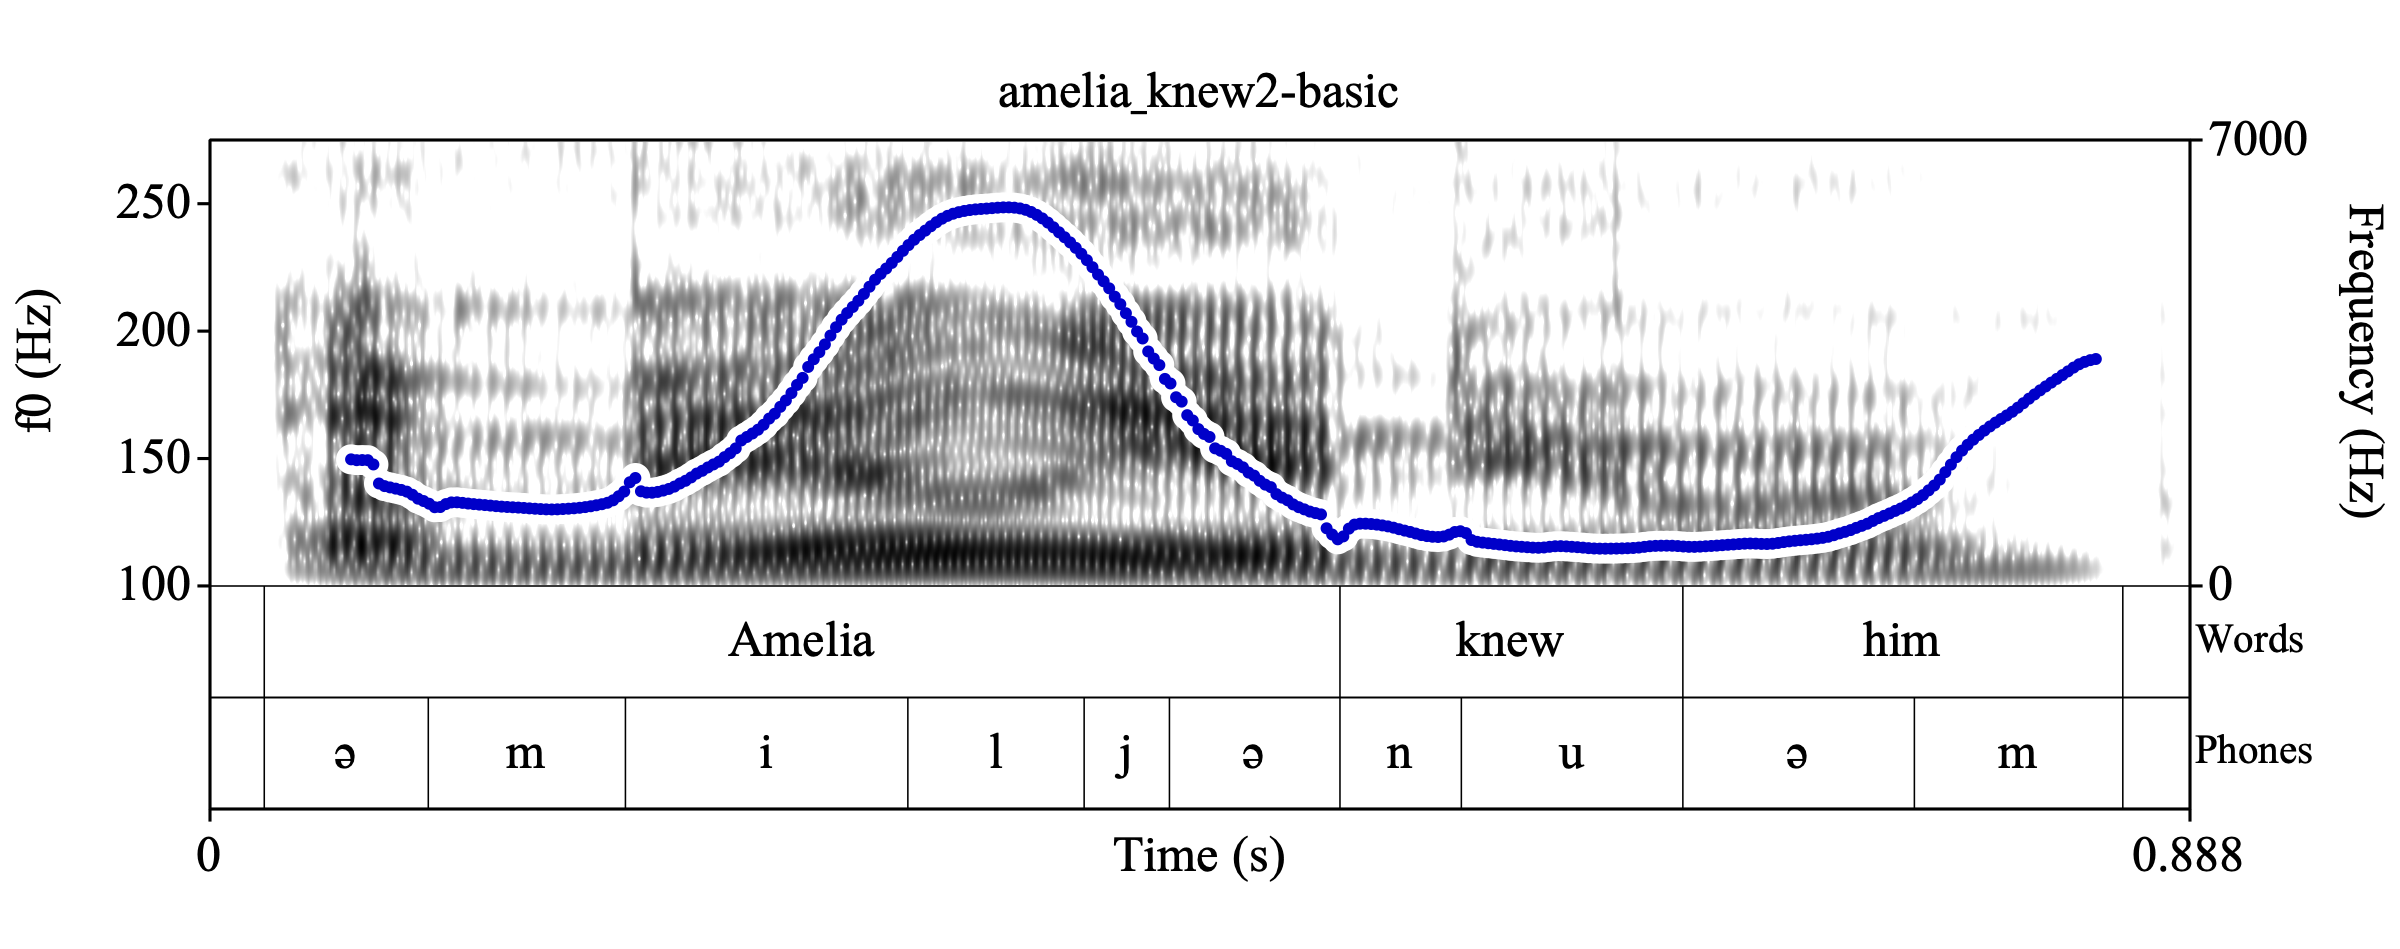
\includegraphics[width=.875\linewidth]{Points-amelia_knew2-f0.png}
%
\caption{The f0 contour for \texttt{amelia\_knew2}.%
\label{fig:amelia_knew2 f0 contour}%
%\index{Annotated example, Points tier (basic)!XXXX}%
}
\end{figure}

One can think of the pitch in the intonational contour as closely related to particular “f0 turning points”. These inflection points in the f0 curve are locations in time where the rate of rise\slash fall changes (that is, the change in the second derivative of the (usually smoothed) f0). The f0 turning points for this last example might be found at the dots below:

\begin{figure}[H]
\centering
%
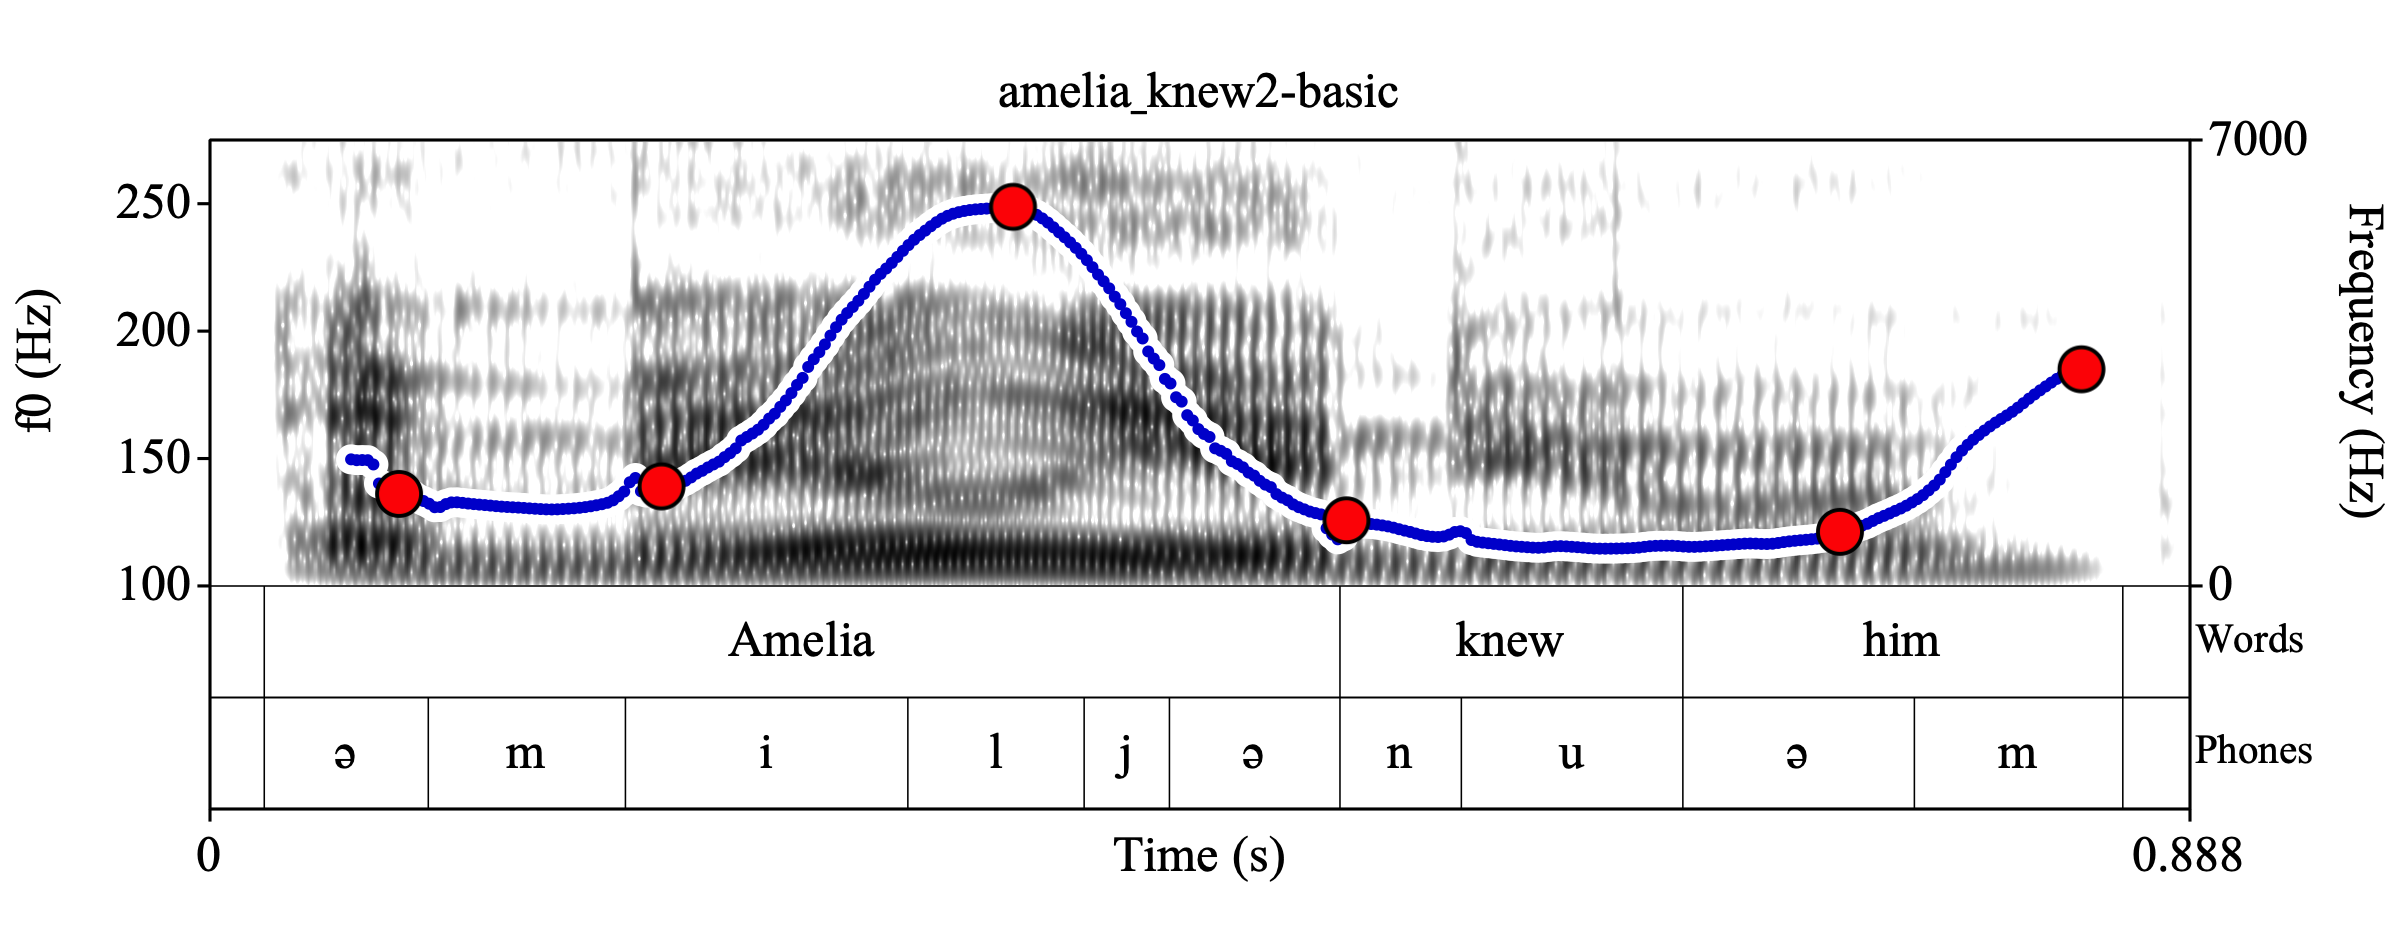
\includegraphics[width=.875\linewidth]{Points-amelia_knew2-f0-dots.png}
%
\caption{The f0 contour for \texttt{amelia\_knew2}, visually annotated for f0 turning points.%
\label{fig:amelia_knew2 f0 contour turning points}%
%\index{Annotated example, Points tier (basic)!XXXX}%
}
\end{figure}

\begin{infobox}[frametitle=\textbf{PRACTICAL SUGGESTIONS}]
 Care must be taken to control pitch settings so that the labelling field is not too wide (“zoomed out”) and that the minimum\slash maximum range choices result in a contour as dynamic and smooth as possible. (See also the discussion of software settings in section \ref{sec:software-effects}.) For discussion of which turning points require labelling, and how to use straight-line-segment resynthesis to aid in making these decisions, see section \ref{sec:points-tier-transcription}.
\end{infobox}

The resulting labels are aligned with these significant turning points on the Points Tier, using the default Basic label ‘\textlabel{0}’ :

\begin{figure}[H]
\centering
%
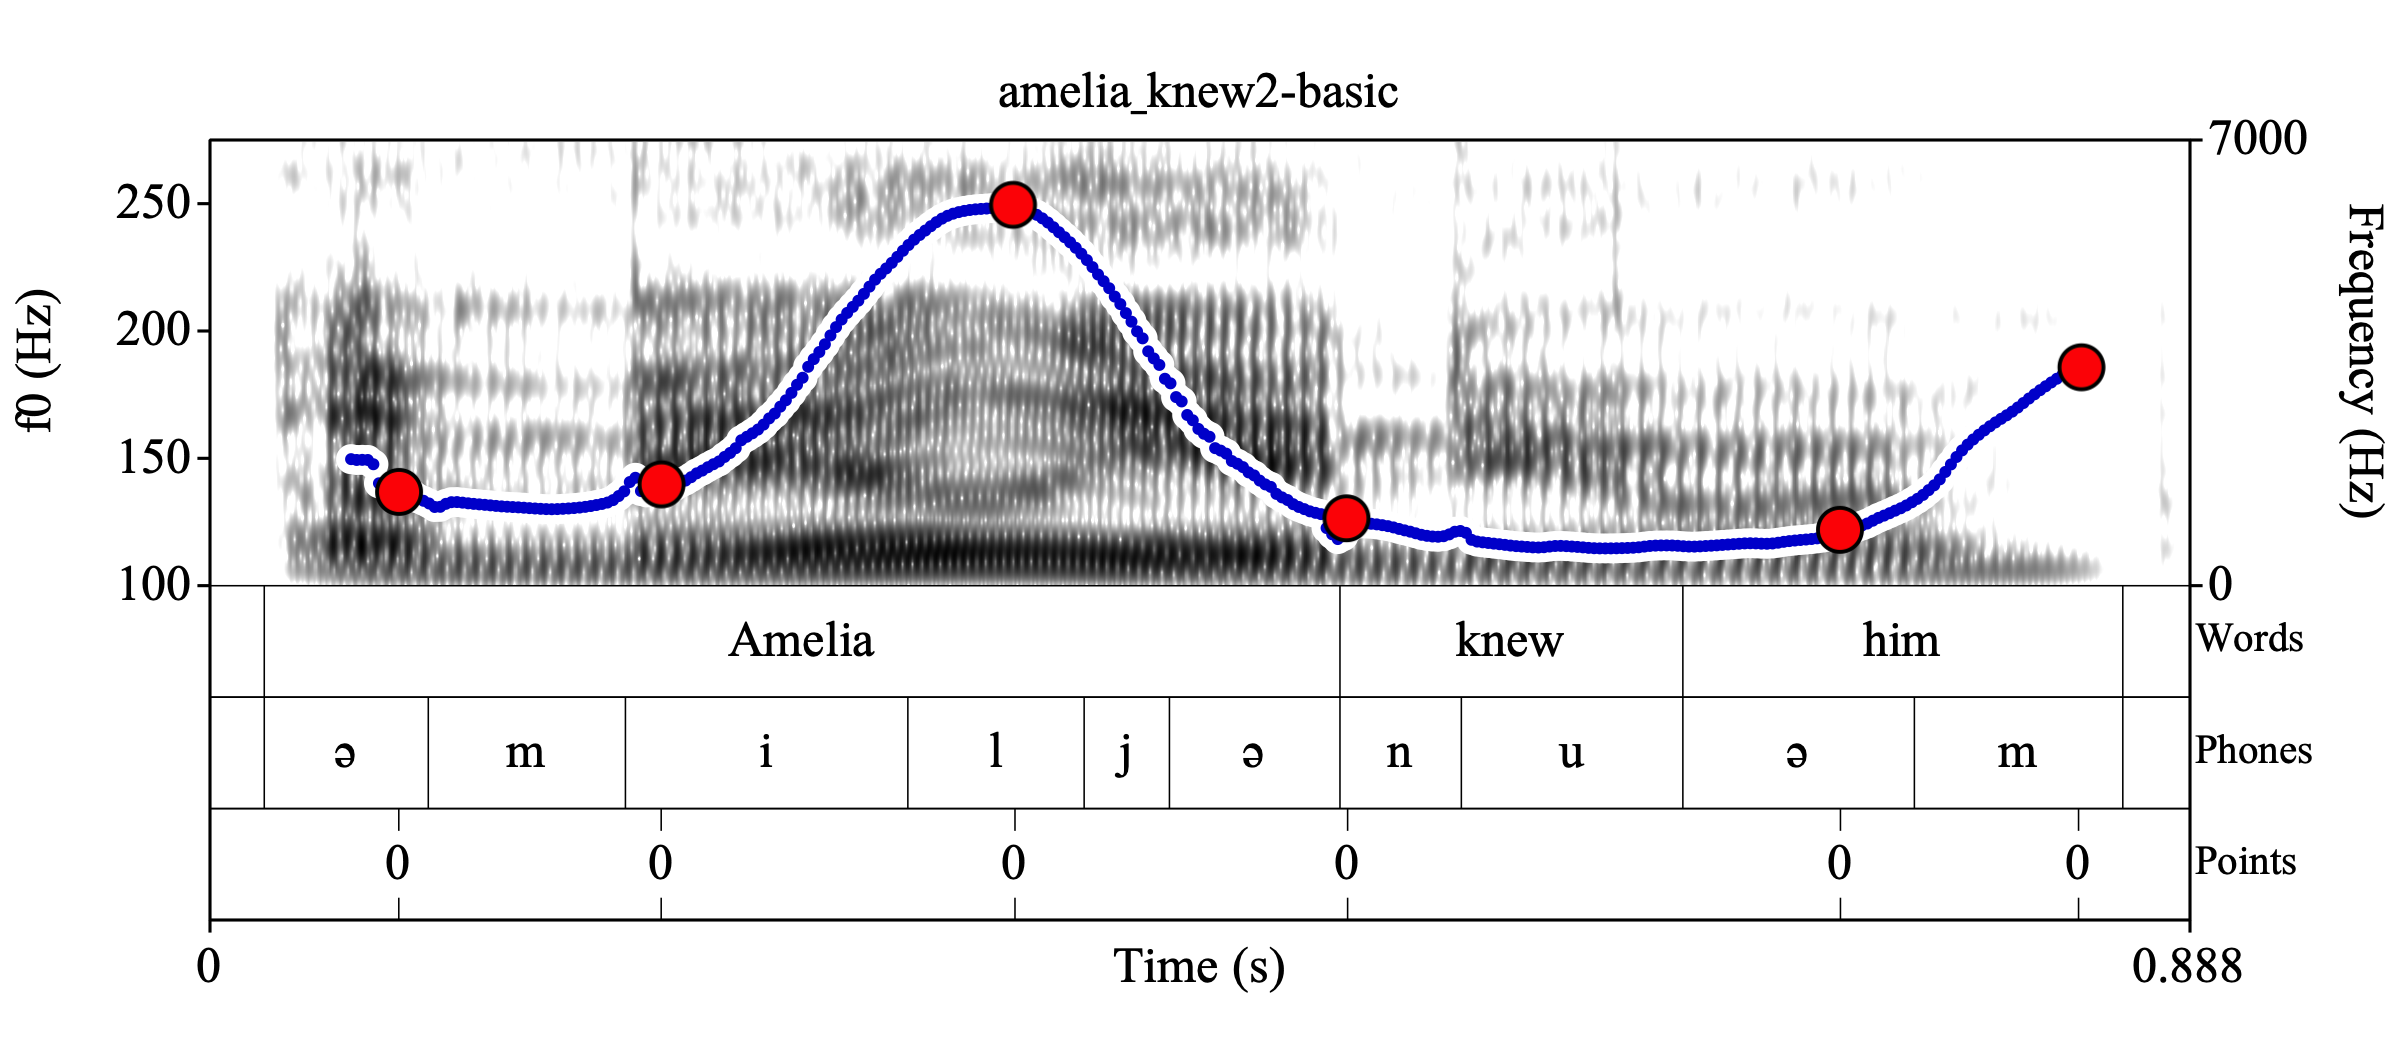
\includegraphics[width=.875\linewidth]{Points-amelia_knew2-basic-dots.png}
%
\caption{The f0 contour for \texttt{amelia\_knew2}, with the Points tier annotated with Basic ‘\textlabel{0}’ labels.%
\label{fig:amelia_knew2 f0 contour turning points 0 labels}%
\index{Annotated example, Points tier (basic)!amelia\_knew2}%
}
\end{figure}

It is important to note that PoLaR allows an annotator to label \uline{\textit{\textbf{any}} (salient) f0 turning point. This contrasts with other,} more phonologically oriented annotation systems (e.g., ToBI, IViE), in which an annotator can only capture a pitch movement by using a label that also indicates an analysis related to the presence of a phonological object.\footnote{As a concrete example, an annotator using such a system can only capture a pitch movement to high pitch if it corresponds to a pitch accent (\textlabel{H*}) or boundary tone (\textlabel{H-} or \textlabel{H\%}). This may be particularly important for the exploration of unfamiliar languages or understudied varieties.} As such, PoLaR intends to capture all significant pitch movements – even those which may not cue a phonological object (at least not in current intonational grammars).\footnote{That is, there may be (potentially systematic) pitch movements that are not predicted by prominence\slash phrasing as we understand them and their relationship to intonation, but which manifest as perceptible movements in the f0 tracking.} We describe more in the next section about what guides whether or not to label a given pitch movement.

\subsubsection{Points Tier Transcription}\label{sec:points-tier-transcription}

The disentangling of turning points from the events labelled on the PrStr tier raises an important question: \textbf{What does and does not get labelled as an f0 turning point?} The answer to this is primarily determined by the main goal of PoLaR’s Points labelling: to capture enough information to identify any\slash all \textbf{systematic patterns} in the f0 curve, without simply replicating the entire curve, point by point, on the Points tier.

In this monograph, we are not aiming to provide an exhaustive account of what should or should not be annotated; instead, we aim to provide \uline{some basic guidelines}. First, is the guideline that the annotator \uline{should not} label f0 movements that are due to the influence of segments\footnote{We do not rule out the possibility of using PoLaR to annotate segmental effects with the goal of learning more about which microprosodic effects are linked to which segments. Indeed, PoLaR would make a good candidate for annotating such changes. However, for general uses of PoLaR, labellers are advised to ignore microprosody. See section \ref{sec:intonational-contours-and-software-based-pitch-tracks} for more discussion.} (sometimes called “microprosody”, even though such f0 movements are not always small), environmental factors (e.g., background noise), or issues with recording-quality (e.g., electrical hums). At the same time, the annotator \uline{certainly should} label all peaks, plateaus, elbows, valleys, etc. that are intonationally salient and/or correspond to PrStr tier objects.

A second guideline to help determine which turning points are perceptually salient is to test the sequence of labelled points in a straight line approximation fidelity test (cf. straight line approximations as implemented by IPO, \citealt{t-hart-90}, and discussed in section \ref{sec:intonational-contours-and-software-based-pitch-tracks}). This test involves \uline{resynthesizing} the pitch of a recording as a sequence of line segments; this is described in the next section.

\subsubsection{Identifying Necessary Points Labels with Straight Line Approximations}\label{sec:identifying-necessary-points-labels-with-straight-line-approximations}

The concept of straight line approximations and a demonstration of how to use Praat to produce one will employ the example above (\texttt{amelia\_knew2}). In Figure \ref{fig:amelia_knew2 resynth}, the original pitch track is shown with a grey dotted line (note its curvature); however, if we use the same points as identified in Figure \ref{fig:amelia_knew2 f0 contour turning points 0 labels} to define the endpoints of line segments, we can get a pitch track as the one shown as the solid green line. Resynthesizing the pitch on the basis of this green line produces an utterance that is perceptually the same as the original. (Audio can be found as \texttt{amelia\_knew2-resynth} on \url{https://www.polarlabels.com}.)

\begin{figure}[H]
\centering
%
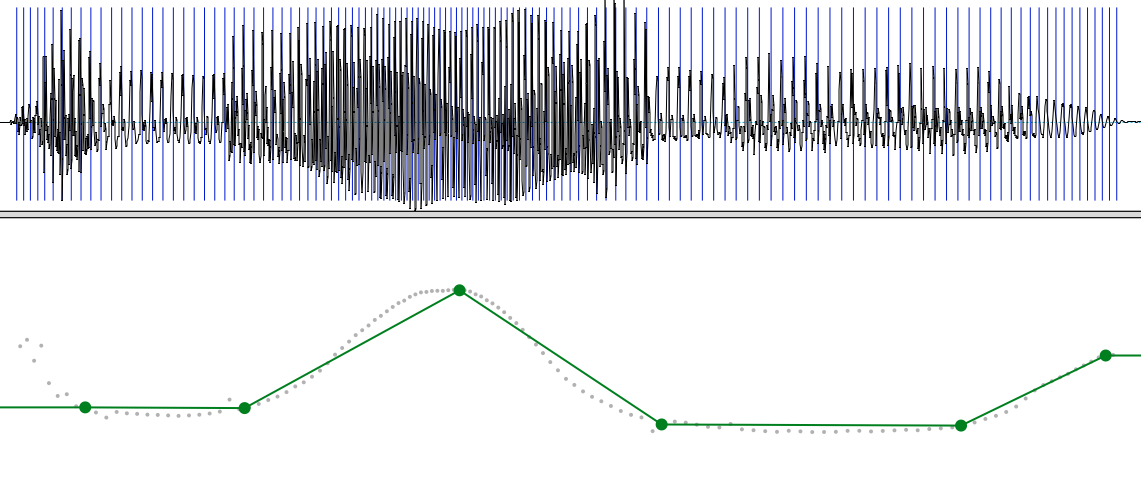
\includegraphics[width=.875\linewidth]{Points-amelia_knew2-resynth.png}
%
\caption{\texttt{amelia\_knew2}, with the resynthesized pitch in green, and the original pitch dotted gray.%
\label{fig:amelia_knew2 resynth}%
%\index{Annotated example, Points tier (basic)!XXXX}%
}
\end{figure}

The PoLaR plugin for Praat (found at the OSF repository linked from \href{https://www.polarlabels.com}{www.polarlabels.com}) automates the resynthesis – though only under the guidance of Points-tier labels provided by PoLaR annotators. (That is, the script is not fully automated, acting on its own; it relies on the human intuition of labellers.) With the plugin installed, users can click on the “Tier” menu and select “PoLaR: Resynthesize Straight Line Approximation”, and this will resynthesize the sound file, based on the pitch track and the timing of the Points tier labels.

\begin{figure}[H]
\centering
%
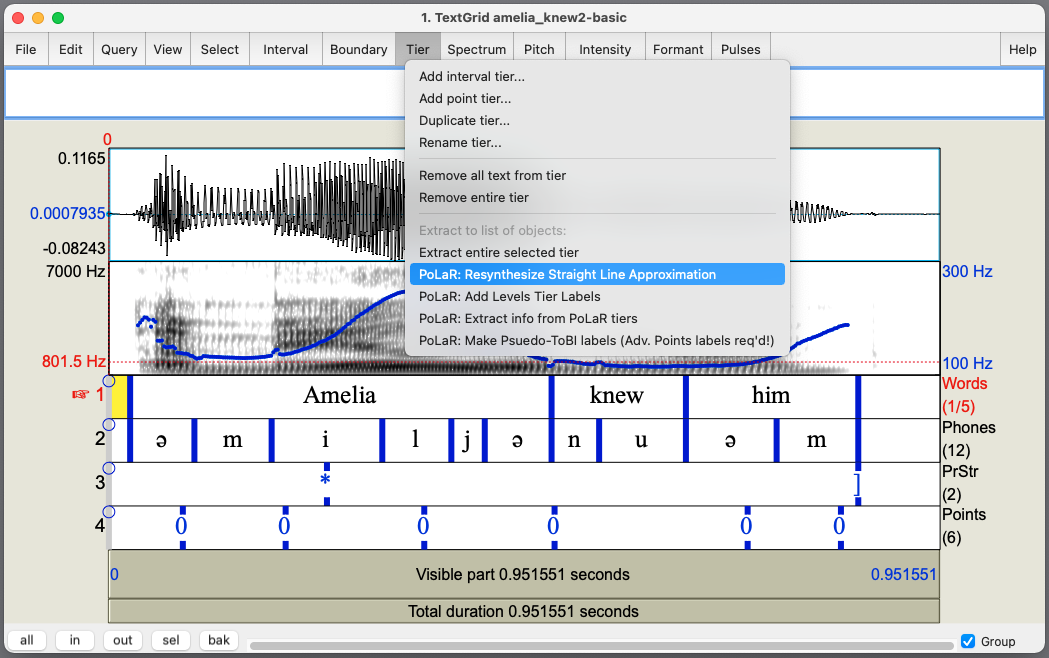
\includegraphics[width=.875\linewidth]{Points-amelia_knew2-before-SLA.png}
%
\caption{Running the Straight Line Approximation script, from the Praat menu in the Editor window.%
\label{fig:amelia_knew2 SLA menu}%
%\index{Annotated example, Points tier (basic)!XXXX}%
}
\end{figure}

This script can be especially useful as a way to test whether a given f0 turning point on the Points tier is necessary to maintain the perceptual equivalence. To use this script to that effect, users can add as many points as they think is necessary at first, run the script, and compare the original and resynthesized versions. If the resynthesized version sounds distinct from the original, users can add\slash remove Points tier labels, and see if this improves the result. An example of this is given in Figure \ref{fig:amelia_knew2 resynth extra}; here the labeller might wonder if they need to have two points towards the peak, to capture that the peak is somewhat rounded at the top. By resynthesizing the pitch with that third point (as in Figure \ref{fig:amelia_knew2 resynth extra}) or without it (as in Figure \ref{fig:amelia_knew2 resynth}), they can compare perception of the two resynthesized recordings to see whether it is necessary.

\begin{figure}[H]
\centering
%
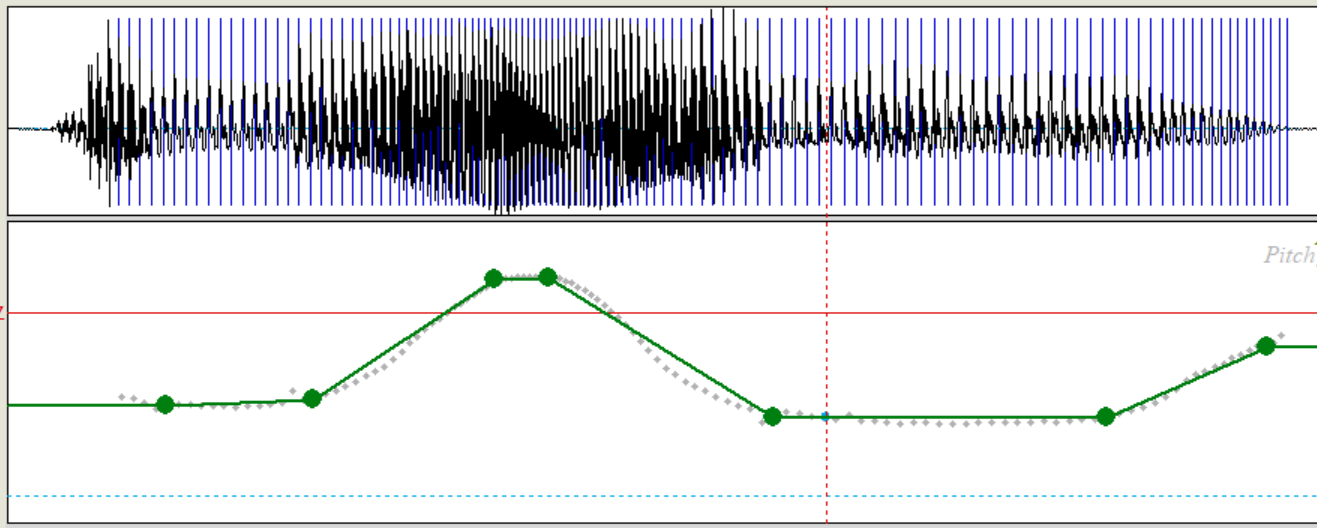
\includegraphics[width=.875\linewidth]{Points-amelia_knew2-resynth-extra.png}
%
\caption[\texttt{amelia\_knew2}, with the resynthesized pitch with an additional point.]{\texttt{amelia\_knew2}, with the resynthesized pitch with an additional point near the f0 peak in green, and the original pitch dotted gray. The addition of the third point makes only an imperceptible change, compared to the resynthesis in the previous figure, and is therefore not needed.%
\label{fig:amelia_knew2 resynth extra}%
}
\end{figure}

As it turns out, these two straight line approximations are perceptually identical. Since the first resynthesis identifies the smaller set of points, and those and only those turning points are perceptually necessary, it is better to label this file with the six turning points in Figure \ref{fig:amelia_knew2 resynth} (and not the seven turning points annotated in Figure \ref{fig:amelia_knew2 resynth extra}). That said, novices should err on the side of over-labelling points as long as they avoid unreliable, noisy f0 points.

One of the contexts where the pitch will often have noisy non-salient turning points is in the case of segmental effects on prosody (“microprosody”). While an experienced labeller may recognize microprosodic perturbations, especially in well known contexts (e.g., around a stop consonant or a sibilant such as [s] or [z]), this may be more difficult for a novice. We will illustrate this briefly here, but the reader is also referred to section \ref{sec:intonational-contours-and-software-based-pitch-tracks} for further discussion. This illustration here concerns the effects of [s]: Compare the pitch tracking surrounding the [s] on “\langtext{nanasanana}” (which was produced with flat pitch, to the point of sounding unnatural) to the pitch tracking of the resynthesized pitch (which sounds identical to the original, to a human ear):

\begin{figure}[H]
\centering
%
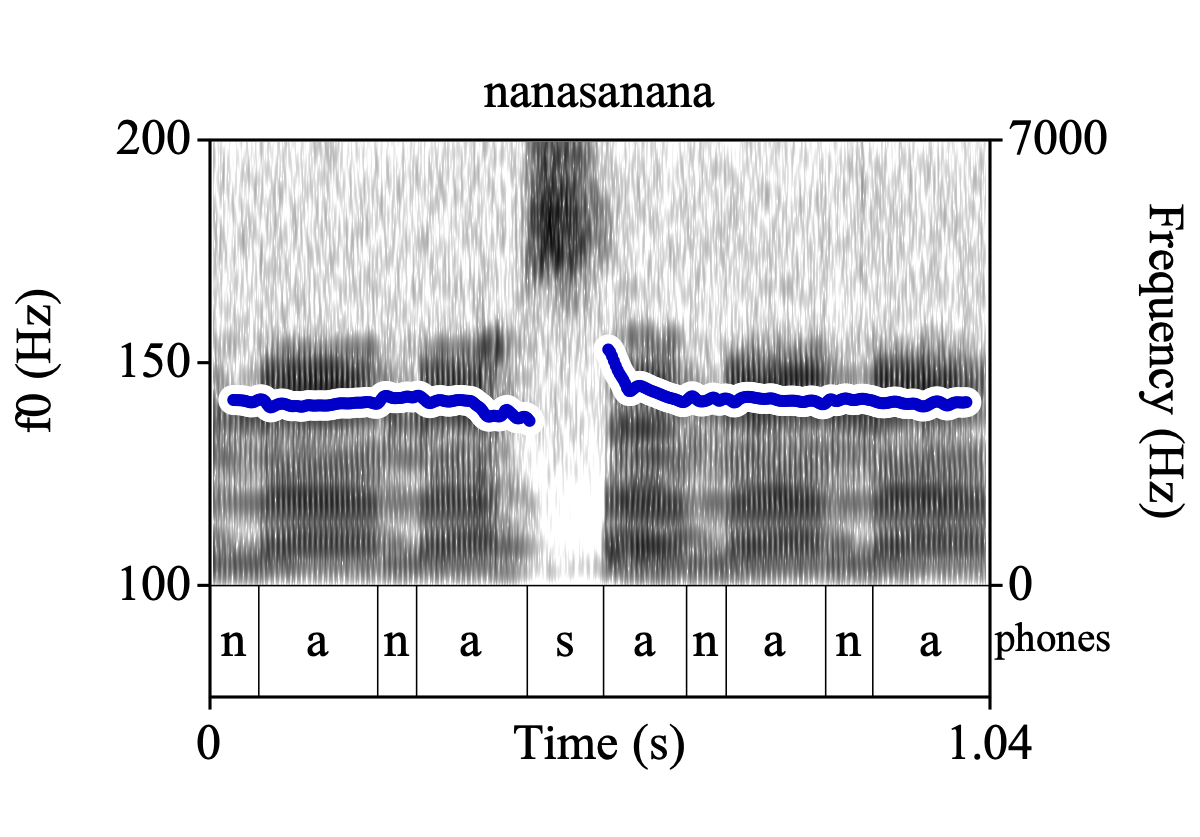
\includegraphics[width=.485\linewidth]{Points-nanasanana.png}~~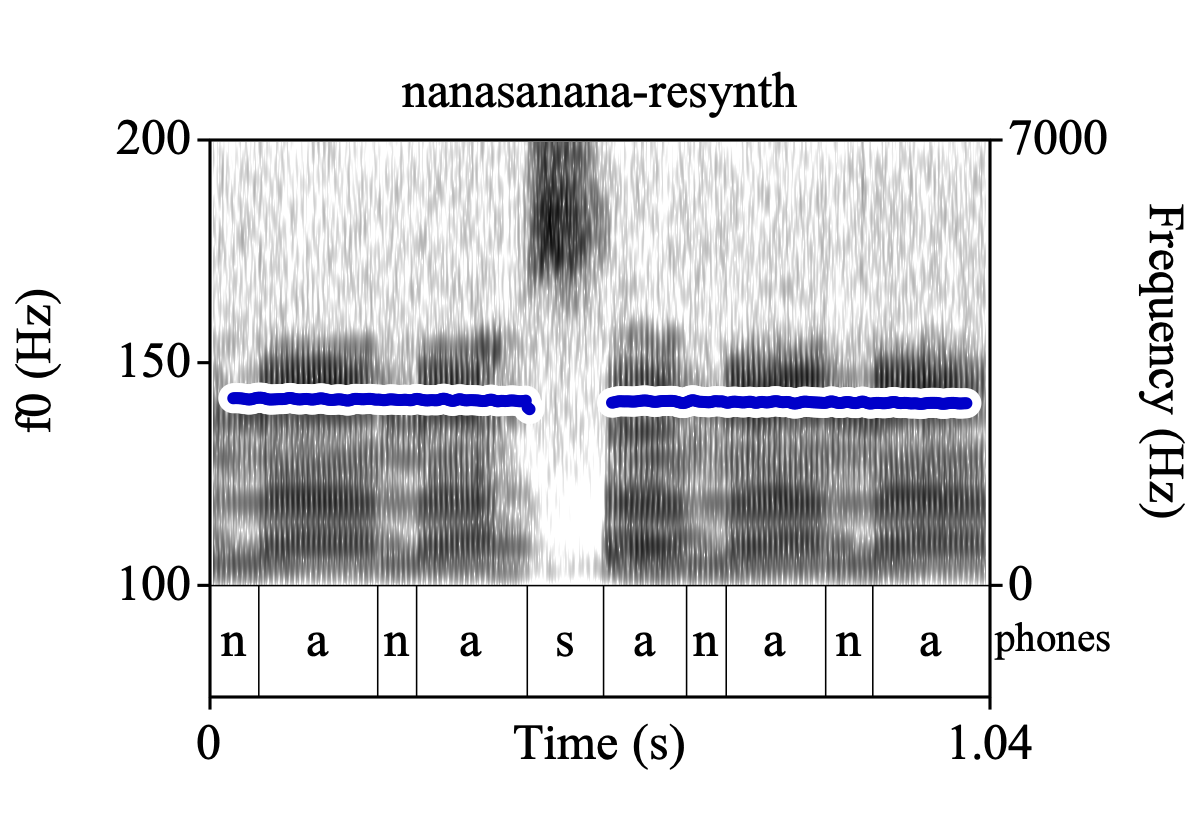
\includegraphics[width=.485\linewidth]{Points-nanasanana-resynth.png}
%
\caption{An original recording (left) and its resynthesized version (right).%
\label{fig:original and resynth}%
}
\end{figure}

The pitch track on the left is the original from Praat. The one on the right has been manipulated and resynthesized in Praat, such that the f0 is a flat line, with the same starting and ending f0 as the original. Listeners generally do not perceive the two audio files in Figure \ref{fig:original and resynth} as different because the f0 movements leading into\slash out of the fricative noise associated with the [s] do not reflect changes in the speaker’s target intonational contour.  Instead, these movements reflect effects of the [s] articulation on the rate of vibration of the vocal folds, and how the software tracks f0. In such cases, where it is clear that the f0 track is influenced by such microprosody, \textbf{the general guideline is to \textit{\uline{not}} put any labels on the Points tier} that would track apparent f0 falls\slash rises that are clearly due to microprosody. In this case, only an initial and final Point would be sufficient to mark the flat f0.

In cases where it is difficult to find \textit{any reliable f0} (e.g., because of microprosodic effects) which may be especially common in the beginning or ends of utterances, section \ref{sec:optional-f0-override-labels-for-annotating-pitch-points-without-a-reliable-f0-track} outlines a solution.

We will return to f0 tracks, intonation contours, and resynthesized straight line approximations in section \ref{sec:intonational-contours-and-software-based-pitch-tracks}.

\subsubsection{Examples of Point Tier labelling}\label{sec:examples-of-point-tier-labelling}

\paragraph{Basic Points Example 1:\label{basic-points-example-1}}

Let us examine a labelled example with a single prominence and a single phrase edge annotated in the Prosodic Structure tier. We will use this example to discuss several aspects of labelling in the Points tier.

\begin{figure}[H]
\centering
%
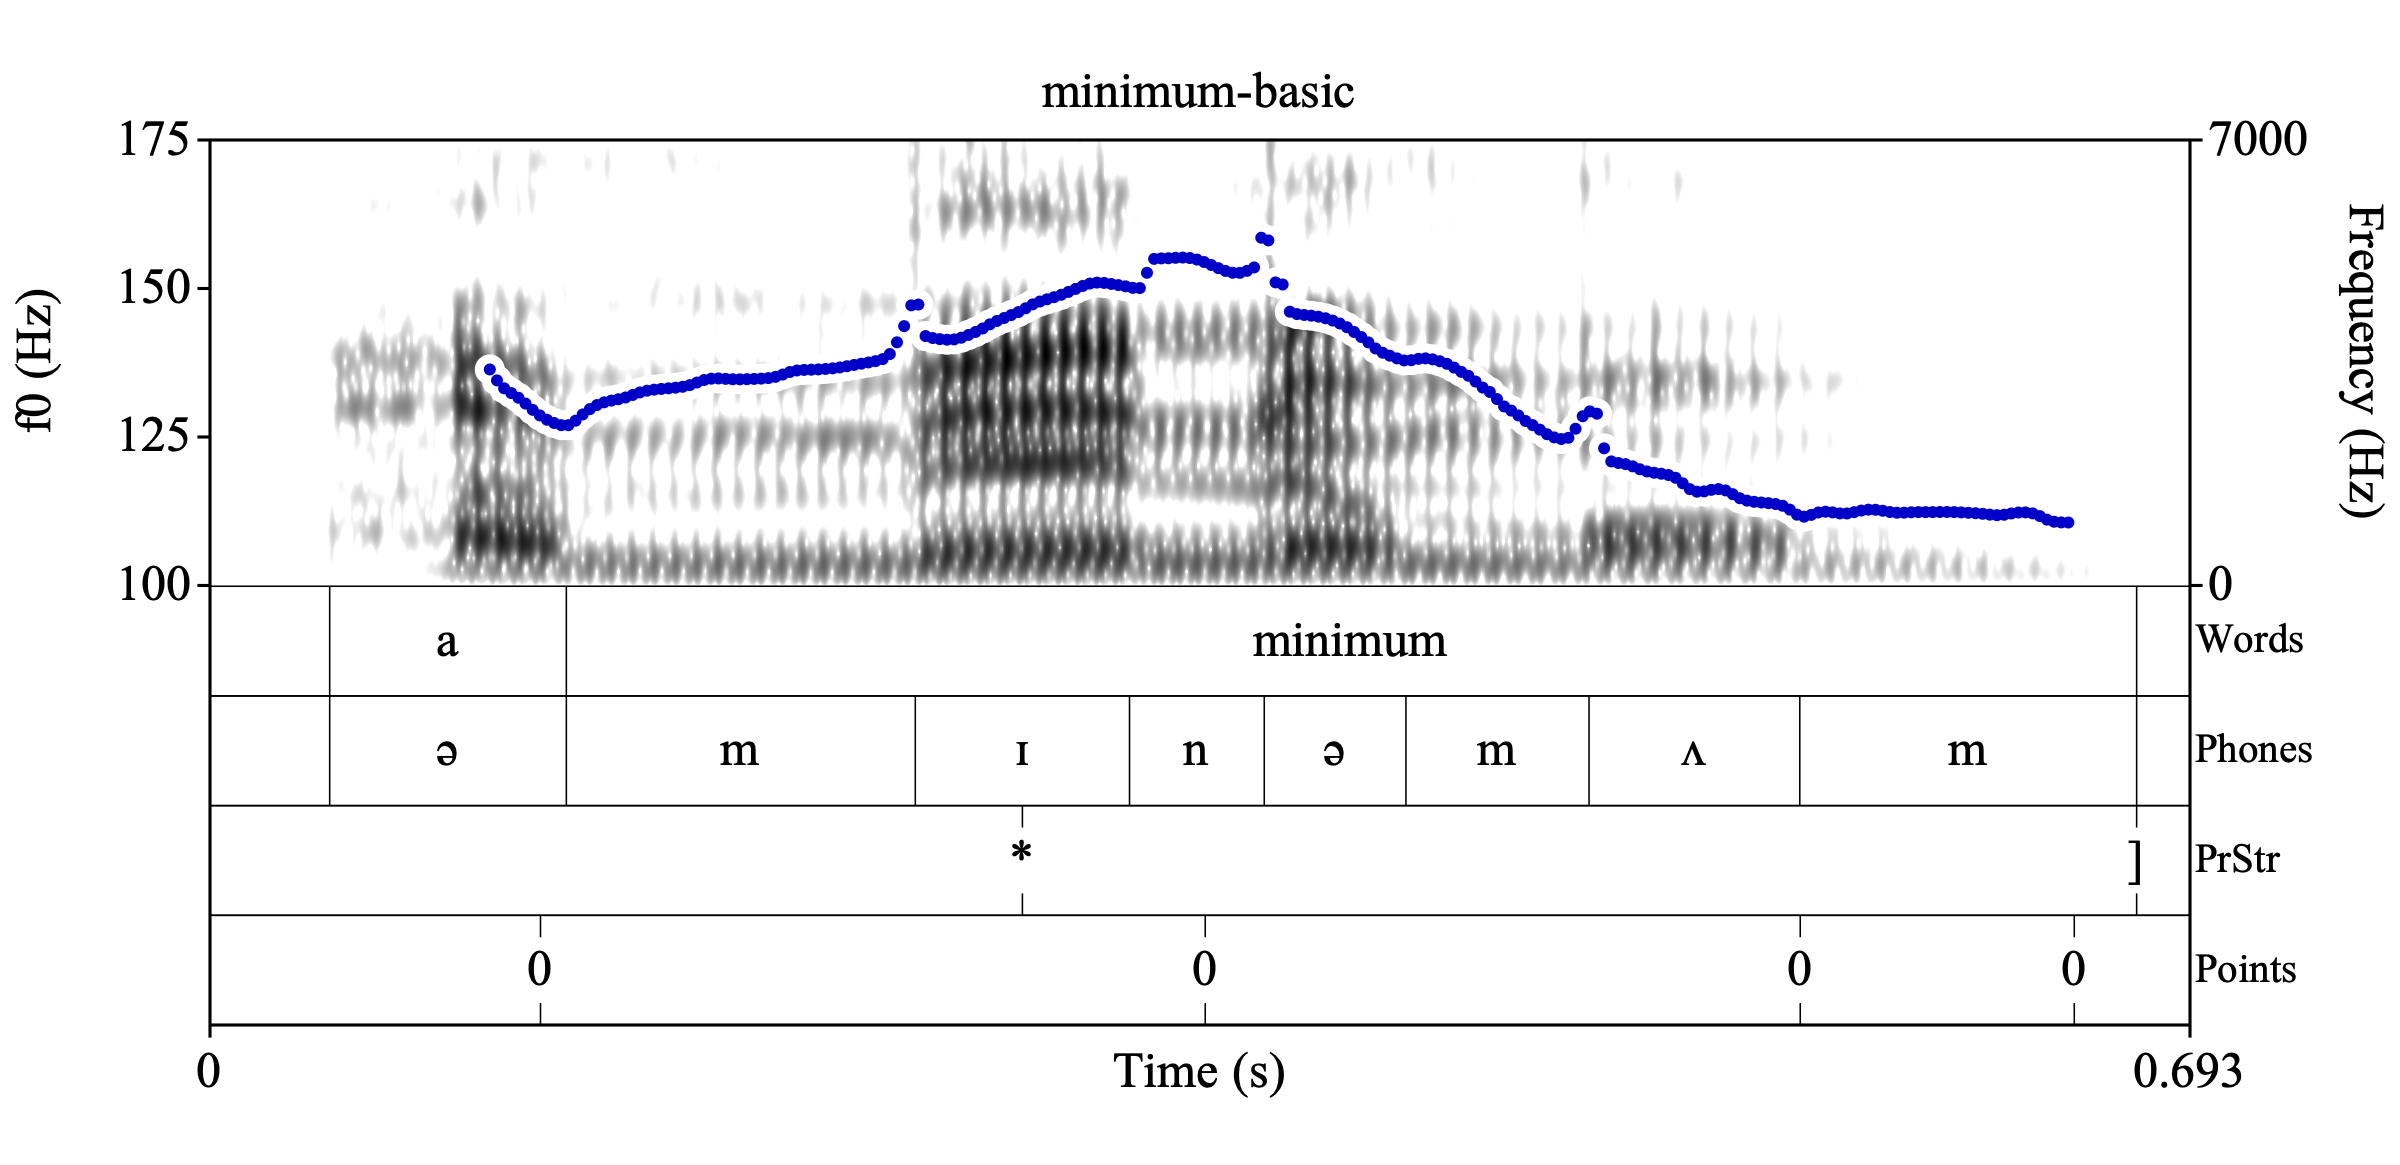
\includegraphics[width=.875\linewidth]{Points-minimum-basic.png}
%
\caption{\texttt{minimum}, with the Points tier annotated with ‘\textlabel{0}’ labels.%
\label{fig:minimum Points basic}%
\index{Annotated example, Points tier (basic)!minimum}%
}
\end{figure}

\uline{First}, note the first (leftmost) ‘\textlabel{0}’ label on the Points tier. It indicates the point in time where (reliable) pitch tracking begins, which corresponds to the beginning of the rise that cues the prominence. (For labellers familiar with other systems like ToBI, take special note that the ‘\textlabel{0}’ default label does not record any relationship between the pitch and the prominence.) Though Praat begins tracking pitch in the middle of “\langtext{a}”, there is no perceptual fall in pitch here, and so we do not want to add a Points label that would produce a falling line at the beginning of the recording. PoLaR labellers are advised to place Points tier labels at the beginning of (reliable) pitch tracking in this way.

\uline{The second ‘\textlabel{0}’ label} is placed at the peak of the f0 track, the location where the pitch again changes direction from rising to falling. Note that the small perturbations between these first two points are not labelled. These are due to noise in the signal processing algorithms and display and are not meaningful in prosodic perception.

\uline{Finally:} The last two points mark the end of the steeper fall and the end of the pitch tract, respectively.

\uline{Overall}, note that the timing of the PrStr tier labels and the timing of the Points labels are completely independent of one another. In the PrStr tier, the \textlabel{*} is aligned to the middle of the stressed vowel, and the \textlabel{]} is aligned to the right edge of the phrase-final word. On the other hand, the Points tier labels are aligned according to the movements of the f0 contour, and not to any particular syllable, word, phrase, etc., and not to any object in the PrStr tier.

\paragraph{Basic Points Example 2:\label{basic-points-example-2}}

In the example in the figure below, the pitch events (rising slightly, falling in two steps) are time-aligned with the default ‘\textlabel{0}’ label.

\begin{figure}[H]
\centering
%
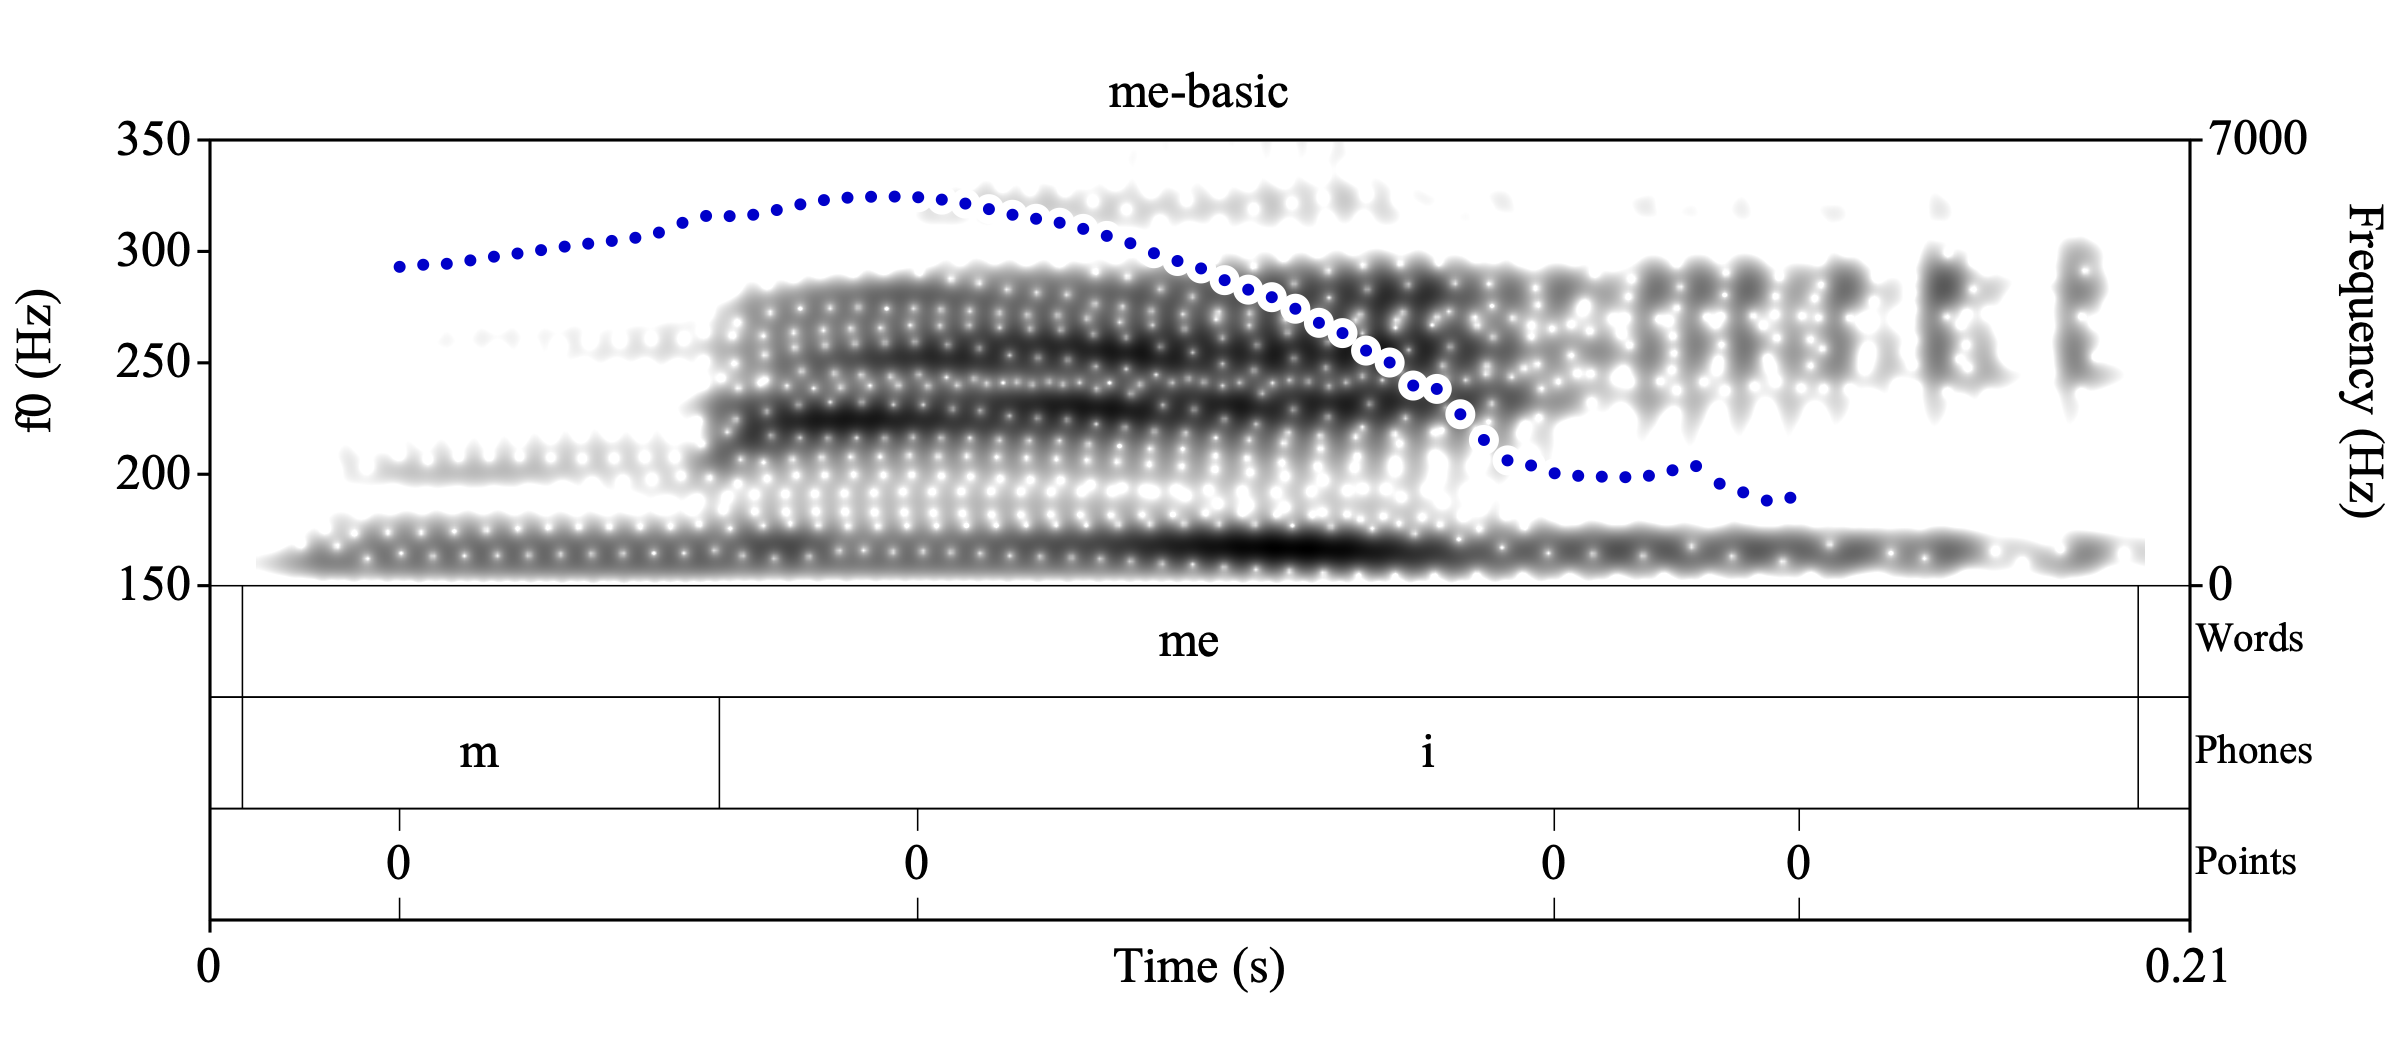
\includegraphics[width=.875\linewidth]{Points-me-basic.png}
%
\caption{\texttt{me}, with the Points tier annotated with ‘\textlabel{0}’ labels.%
\label{fig:me Points basic}%
\index{Annotated example, Points tier (basic)!me}%
}
\end{figure}

Note the timing of the last two labels on the Points tier. The third ‘\textlabel{0}’ occurs where the f0 curve changes trajectory radically, as expected. However, the final ‘\textlabel{0}’ does \textit{\uline{not}} occur at the end of the recording or at the final phrase break (] in the PrStr Tier), because the f0 tracking stops before the recording does. In such a situation, one can simply place the ‘\textlabel{0}’ label where the f0 track ends (or stops being reliable, in the sense of reliably tracking perception of the intonational contour).

\paragraph{Basic Points Example 3:\label{basic-points-example-3}}

Other types of pitch movements might present challenges where the pitch contour displays discontinuities and turns that are not perceptually salient, at least not with respect to the overall perception of the intonation. For example, consider the pitch track below.

\begin{figure}[H]
\centering
%
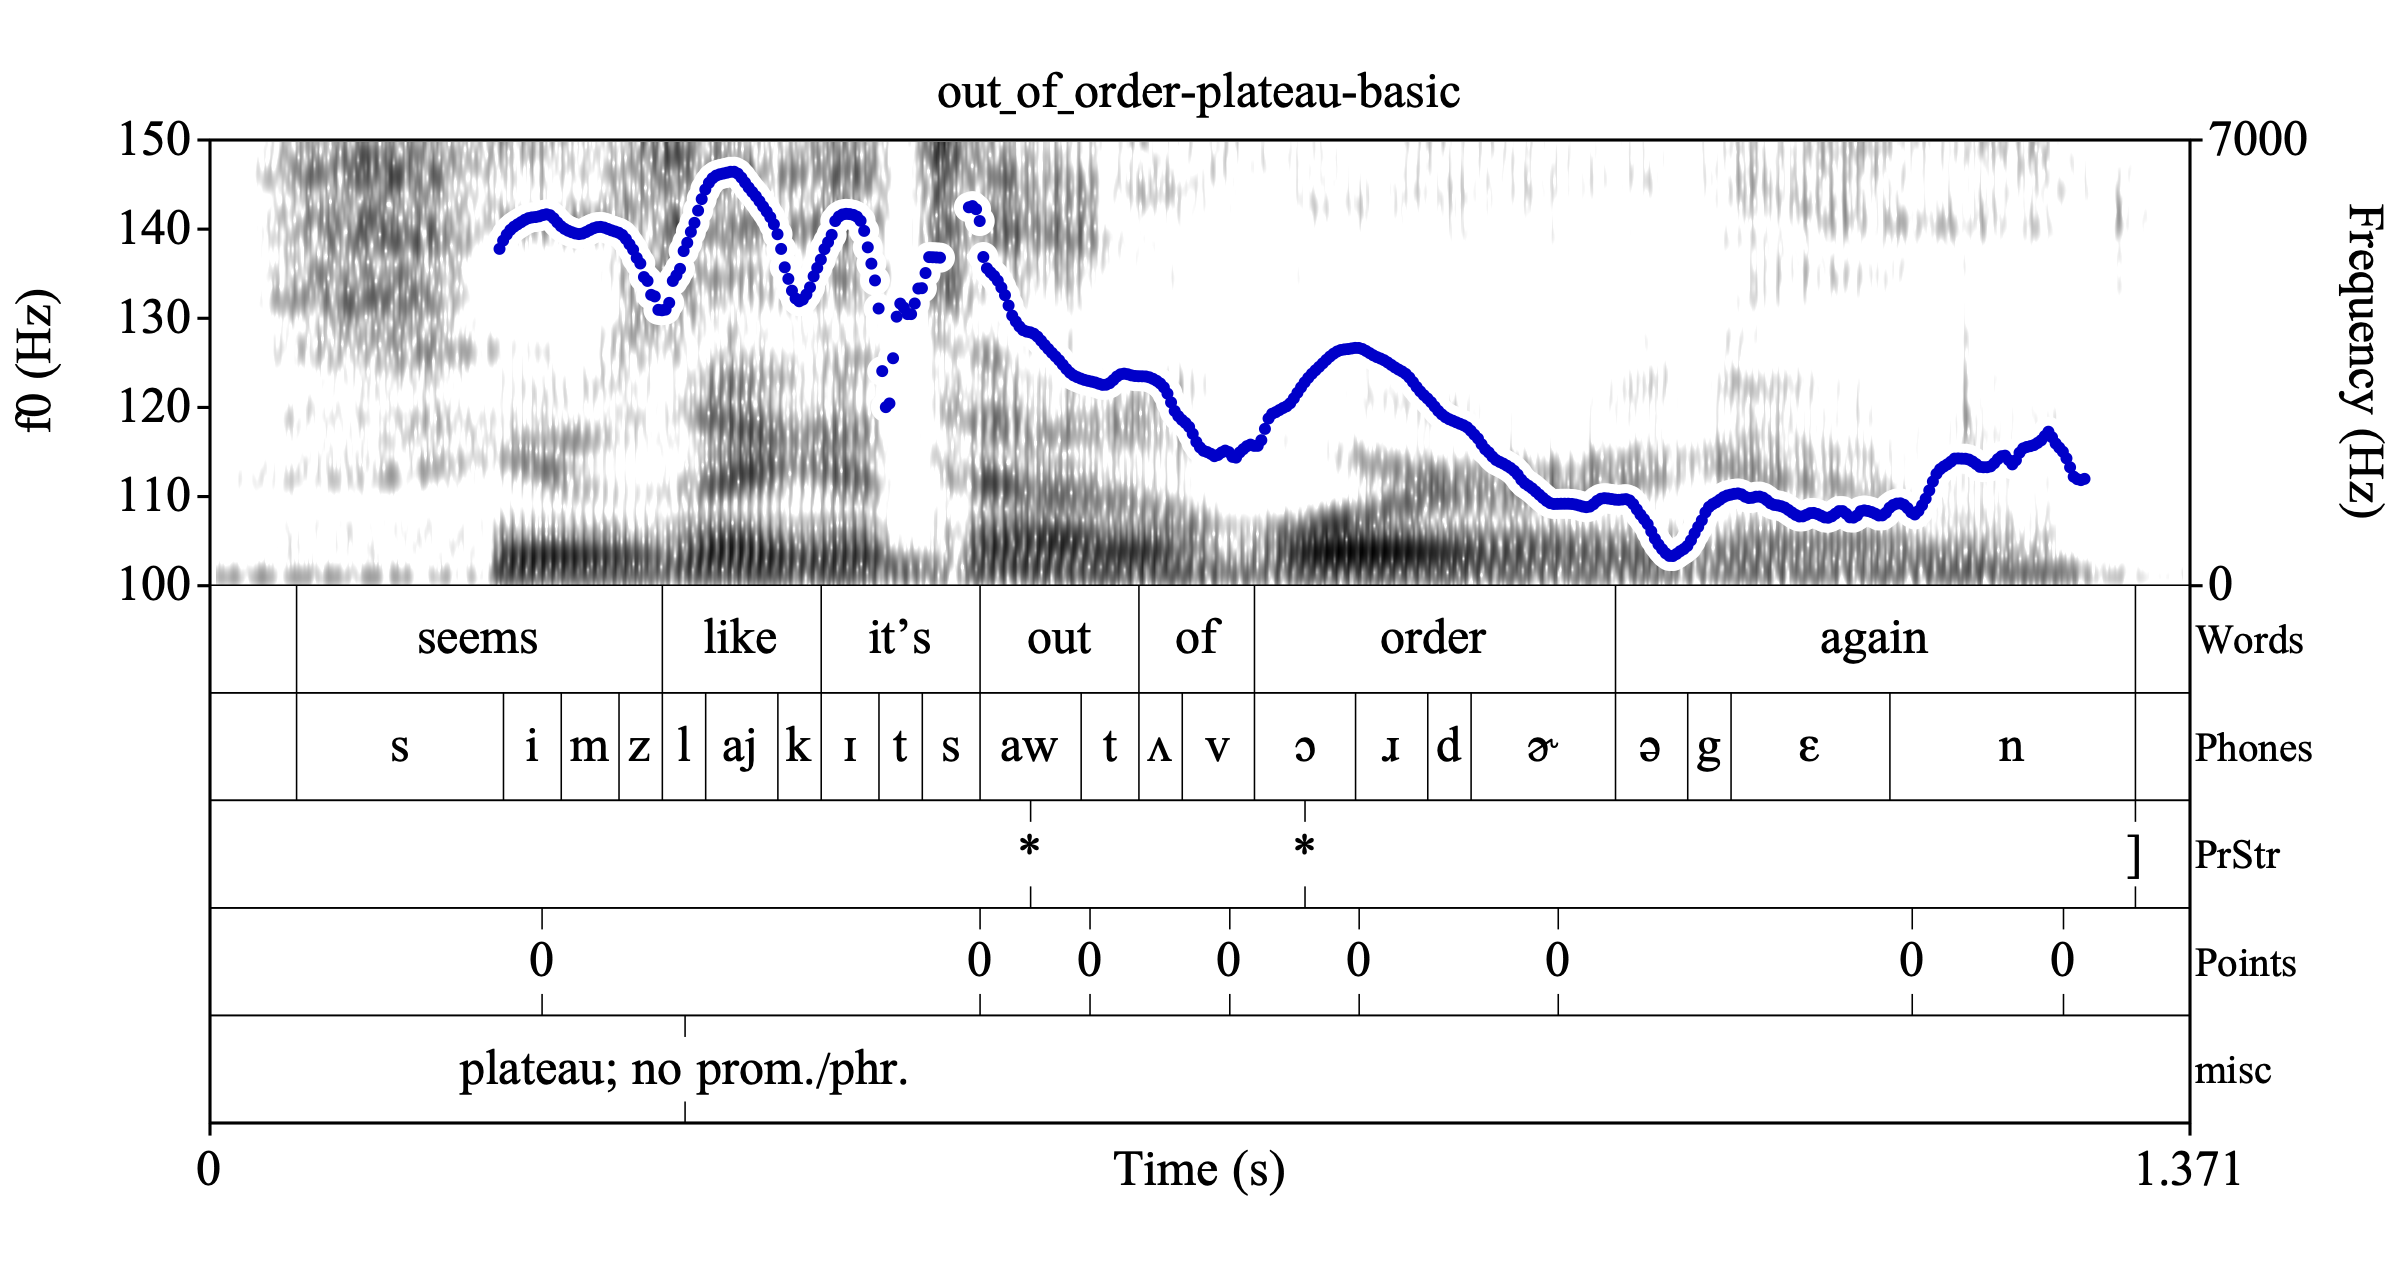
\includegraphics[width=.875\linewidth]{Points-out_of_order-plateau-basic.png}
%
\caption{\texttt{out\_of\_order-plateau}, with the Points tier annotated with ‘\textlabel{0}’ labels.%
\label{fig:out_of_order-plateau Points basic}%
\index{Annotated example, Points tier (basic)!out\_of\_order-plateau}%
}
\end{figure}

Labellers report hearing a steady high pitch at the beginning of the utterance, from “\langtext{seems}” through “\langtext{it’s}” despite the  visible pitch perturbations in the f0-tracking. Moreover, labellers do not perceive any prominence or juncture that would call for a \textlabel{*} or \textlabel{]} label. In order to capture this long, high plateau, points tier labels have to be placed only at the beginning and end  of this interval. This will also reproduce the plateau in a straight line approximation, such as the one created with the PoLaR Praat plugin’s “Resynthesize Straight Line Approximation” command (described in section \ref{sec:identifying-necessary-points-labels-with-straight-line-approximations}), shown in Figure \ref{fig:out_of_order-plateau Points basic resynth}.

\begin{figure}[H]
\centering
%
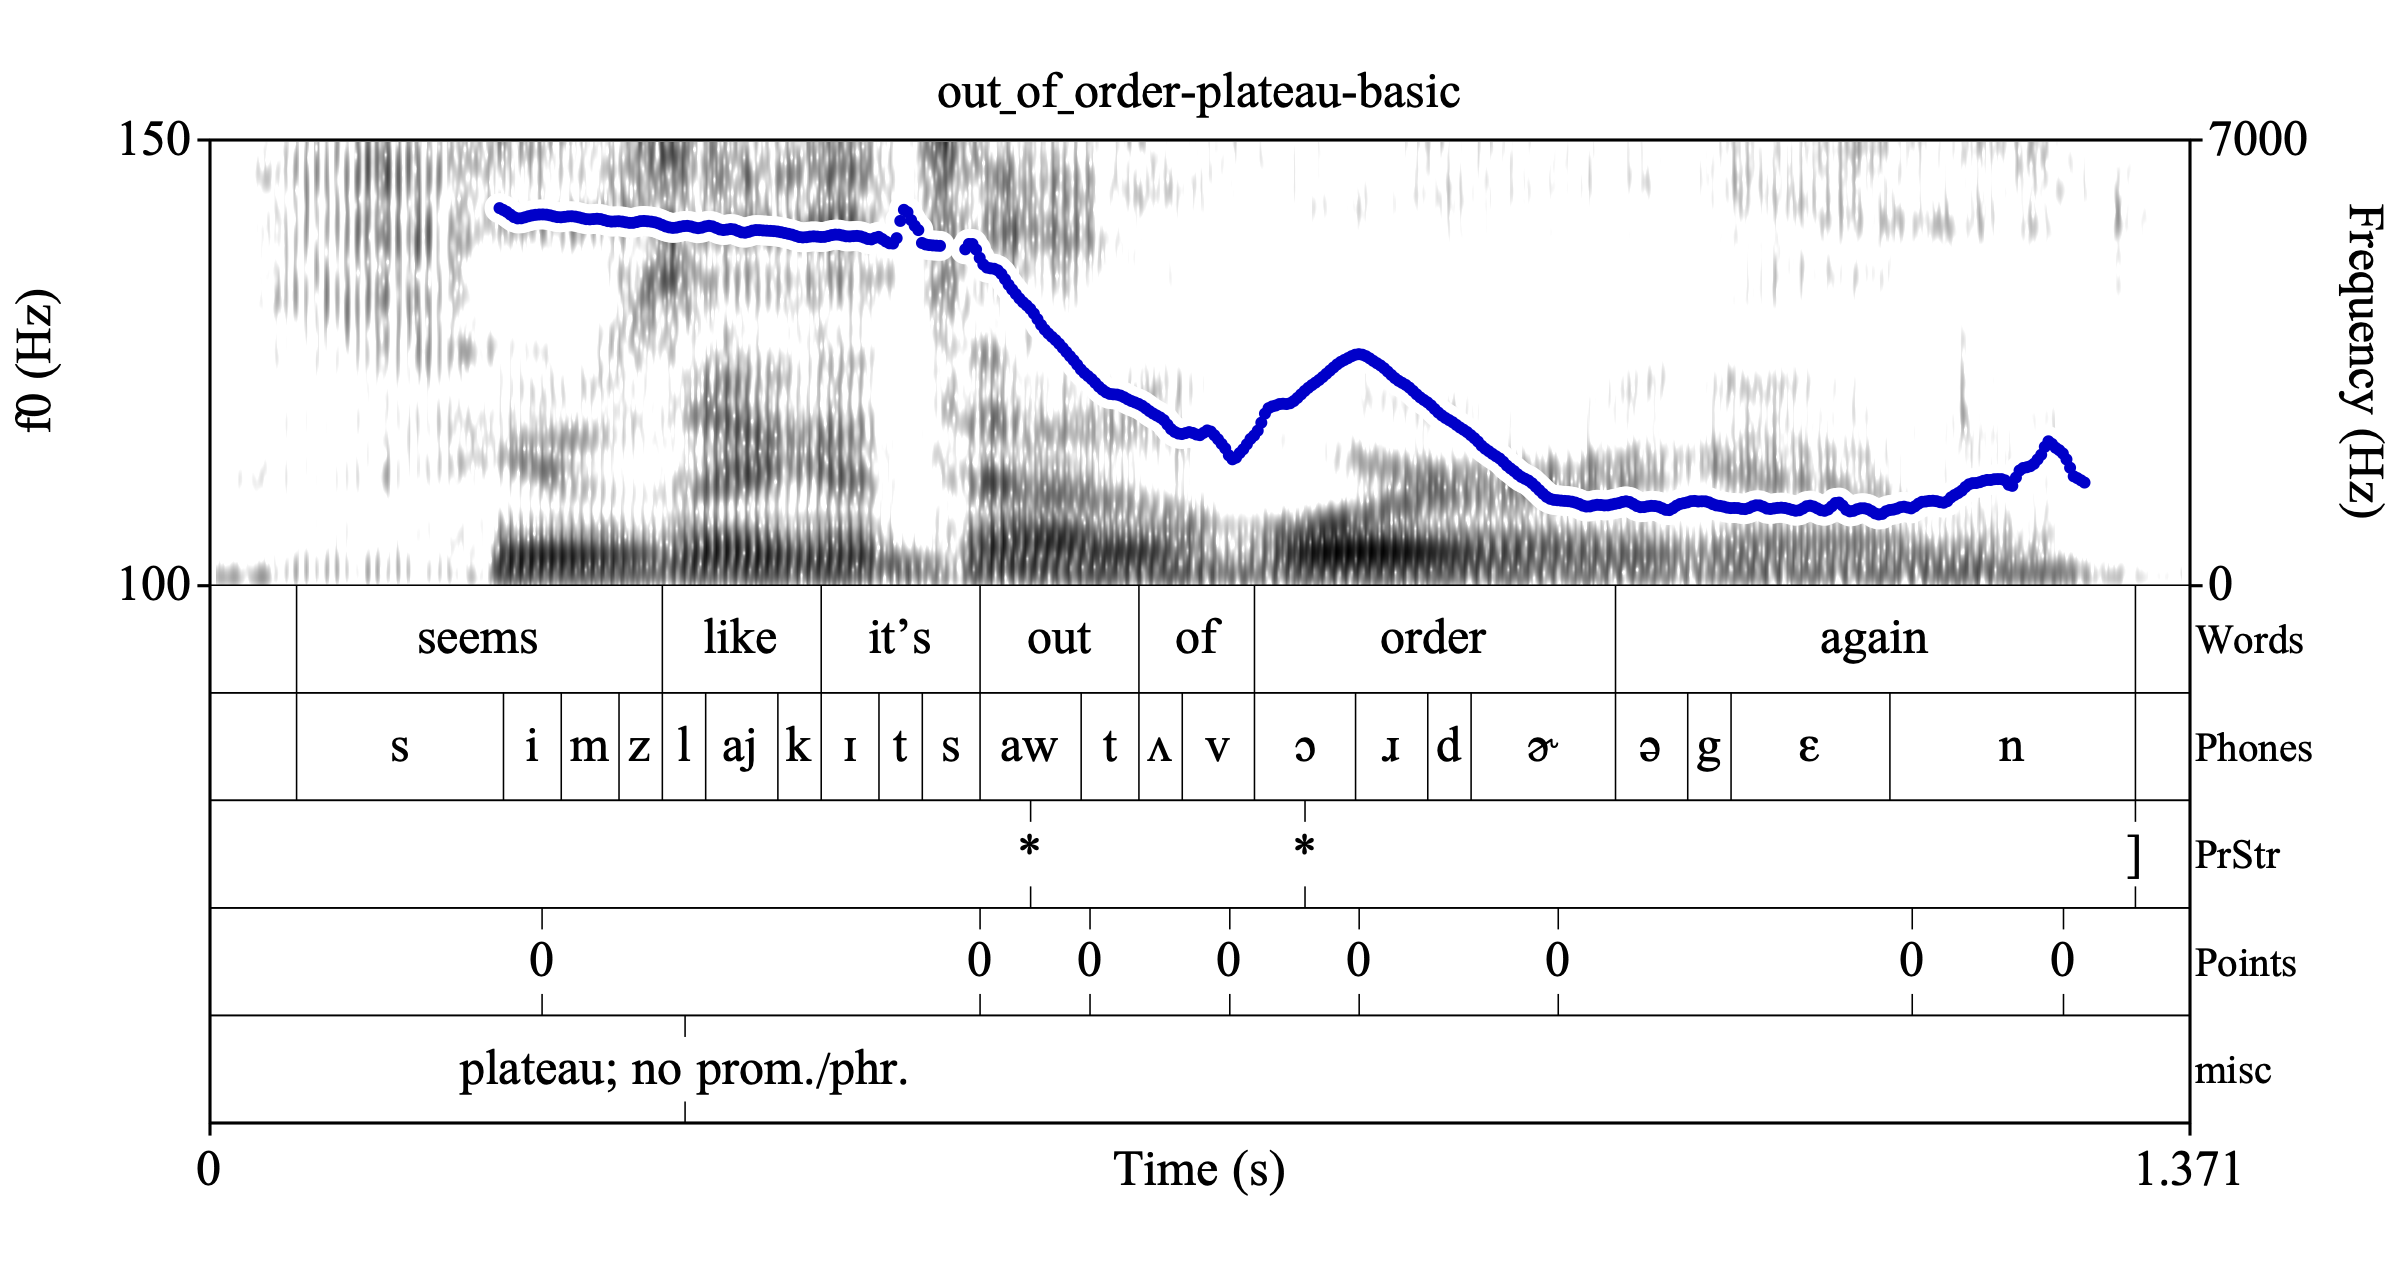
\includegraphics[width=.875\linewidth]{Points-out_of_order-plateau-resynth-basic.png}
%
\caption[\texttt{out\_of\_order-plateau-resynth} is a resynthesized straight-line approximation that is perceived as sounding intonationally the same as the original recording, \texttt{out\_of\_order-plateau}.]{\texttt{out\_of\_order-plateau-resynth} is a resynthesized straight-line approximation that is perceived as sounding intonationally the same as the original recording, \texttt{out\_of\_order-plateau}. (Note that this SLA is not precisely “straight”, despite being resynthesized. This highlights the effect of the signal detection algorithm, even from a source where f0 has been artificially manipulated to consist of straight line segments. Motto: do not place undue trust onto the visual display of the f0 contour.)%
\label{fig:out_of_order-plateau Points basic resynth}%
\index{Annotated example, Points tier (basic)!out\_of\_order-plateau}%
}
\end{figure}

Listeners hear the original recording as sounding intonationally the same as the resynthesized version, corroborating that the pitch tracking in the original recording is unreliable.

With experience, annotators need not resynthesize every turning point to ascertain its validity. In fact, labelling too many turning points is preferable to labelling too few. However, if one were to visually (or with a very simple automatic script) identify all of the f0 turning points in most utterances, there are likely to be more than are necessary to generate an appropriate straight line approximation. Many of these turning points will be typical segmental perturbations or other noise in the signal.

\paragraph{Basic Points Example 4:\label{basic-points-example-4}}

An example of this is below; attend to the fact that there are no Points tier labels in or near the word “\langtext{not}”, (even though it is perceived as prominent):

\begin{figure}[H]
\centering
%
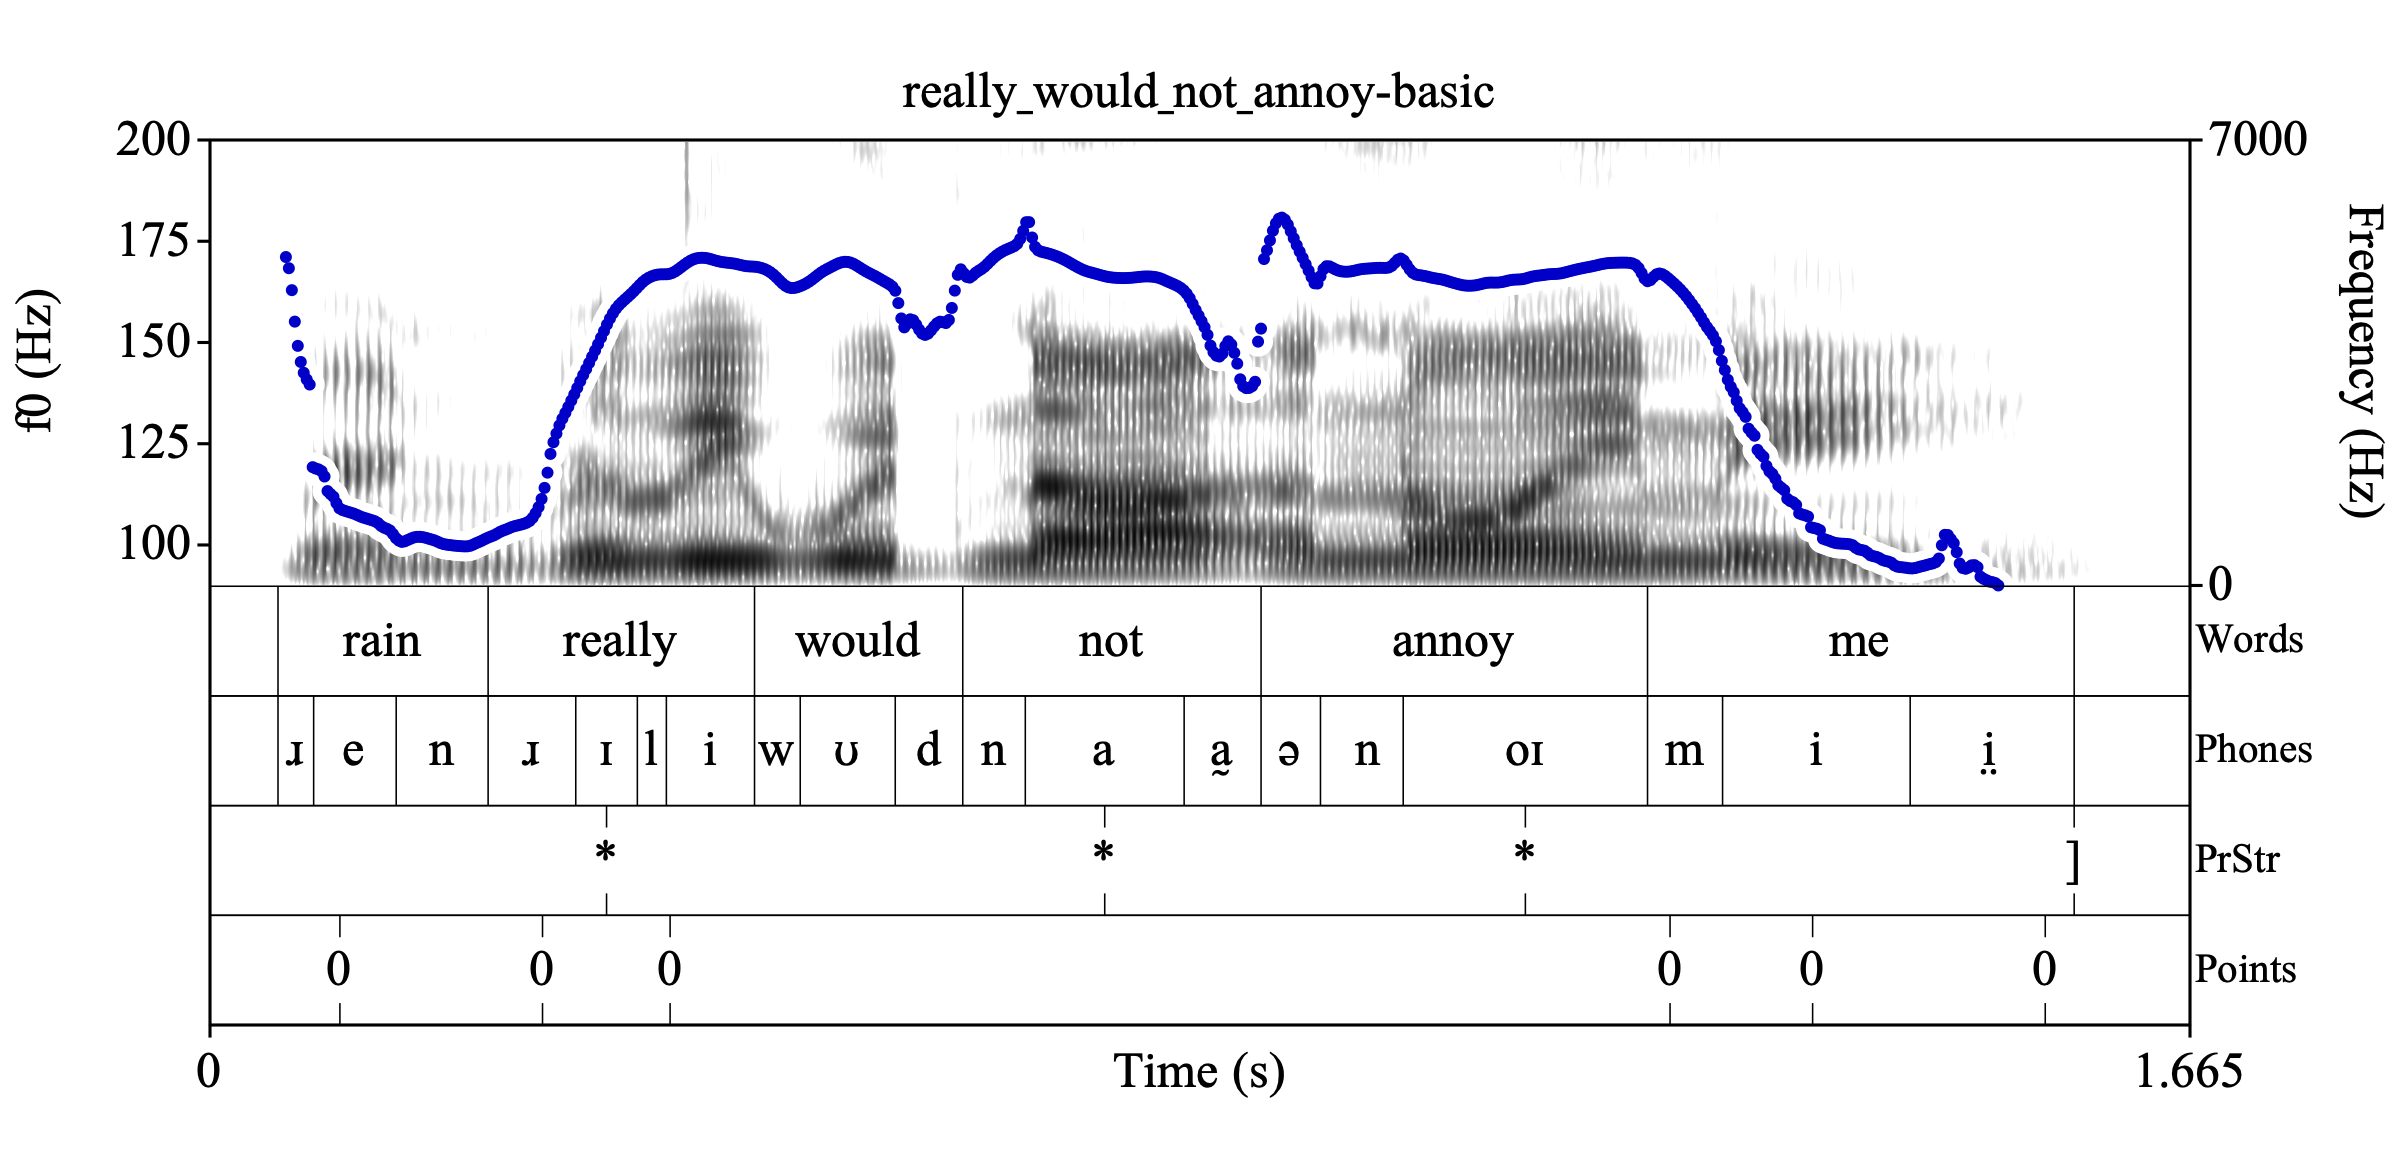
\includegraphics[width=.875\linewidth]{Points-really_would_not_annoy-basic.png}
%
\caption{\texttt{really\_would\_not\_annoy}, with the Points tier annotated with ‘\textlabel{0}’ labels.%
\label{fig:really_would_not_annoy Points basic}%
\index{Annotated example, Points tier (basic)!really\_would\_not\_annoy}%
}
\end{figure}

The small perturbations along the otherwise flat f0 track from “\langtext{really}” through “\langtext{annoy}” are microprosodic or noise related and are also not labelled. Listeners hear this interval as a sustained high tone and not as 2-3 separate peaks. Also note that the leftmost ‘\textlabel{0}’ has been placed at the location of the first reliable f0. In this case, that label is not at the beginning of the f0 tracking; instead, its placement is meant to indicate that the labeller does not believe that f0 track produced by the software is accurate until a bit into the vowel of “\langtext{rain}”.


\subsubsection{Labeller Uncertainty}\label{sec:labeller-uncertainty-points}

As was the case when labelling prosodic events in the PrStr Tier, labellers might be uncertain about whether an f0 turning point exists. In many of these cases, using the Straight Line Approximation Tool or the Override Labels described in the next section can resolve these issues. However, if neither approach is helpful, the labeller can again employ the ‘\textlabel{?}’ (as in ‘\textlabel{?0}’) to indicate that there might be a turning point at this location but it is not certain.

\subsubsection{Optional f0 Override Labels for Annotating Pitch Points without a (Reliable) f0 Track}\label{sec:optional-f0-override-labels-for-annotating-pitch-points-without-a-reliable-f0-track}

At this point, we have discussed how software-produced f0 tracks may not have a direct correspondence to pitch perception (as in, e.g., cases where the f0 tracking disappears or jumps around). In this section we describe a method that a labeller can use to address this problem, by adding a Points label that can be informative for later analysis.

There are multiple reasons why a pitch track may be discontinuous or display faulty f0 points. First, f0 is the measurement of the vocal fold vibration rate (“voicing”) and there are naturally occurring speech events where the vocal folds don’t vibrate (e.g., voiceless segments such as [f]) or they vibrate irregularly (“creaky” voice). While this produces gaps in regular vocal fold vibration, many of these are “corrected for” by the human perceiver, who perceives the pitch as continuous and steady.

In addition, the f0 pitch tracking display itself (in software like Praat) might be inaccurate due to the software f0-tracking settings. Most speech applications require some calibration for each speaker, so that f0 displays are as accurate (and as easily read) as possible. For example, inappropriate settings for the maximum f0 value and/or the minimum f0 value under Praat’s “Pitch settings” can lead to pitch halving\slash doubling (in which the reported f0 value is half or double of the “true” value), while inappropriate settings for the voicing threshold and octave jump costs can lead to f0 dropout or spurious f0 readings.

Lastly, there may also be portions of a recording where there is interference from environmental\slash recording factors, disrupting the f0 tracking algorithms.

These are just some of a few reasons that a pitch track may not always be reliable. (For further discussion of these phenomena, and examples of them, see section \ref{sec:intonational-contours-and-software-based-pitch-tracks}.) At the same time, it is sometimes the case that a labeller can induce where the pitch track “should” be, even when automatic f0 estimates are misleading or f0 cannot be measured at all. This induction is possible because of the way human speech perception works (as mentioned above), and it is aided by visual tools like (partial) f0 tracks that the software can provide. \textbf{To put it more briefly: it is possible that a labeller may have an intuitive sense of where (in time and frequency) a pitch turning point sits, better than the f0 tracking software.}

For this reason, PoLaR provides a means for a labeller to “override” the f0 tracking, and annotate the f0 value that they intuit in the Points label. To annotate this, the labeller adds a comma and the intuited f0 value after the Points label: for example, ‘\textlabel{0,98}’ on the Points tier indicates there is a pitch turning point at this time, and the f0 should be treated as 98Hz (instead of whatever f0 value the software tracker finds). Examples of these “\textbf{comma override}” labels on the Points tier are provided below.

Before getting to the examples, let’s review three reasons that these comma annotations should be used.
\begin{enumerate}
	\item One reason to use them is to ensure that future analysis of the f0, which runs on the basis of PoLaR labels, is reliable. (That is, to minimize misleading measurements that result from f0 tracking errors.)
	\item A second, related reason is that f0 at the end of an utterance is very often creaky and therefore unreliable; thus a Points label without a comma override value might lead to inappropriate f0 values, leading to issues with analysis, straight line approximation resynthesis, etc.
	\item The last, somewhat practical  reason is that various PoLaR scripts and tools, such as the straight-line approximation resynthesizer (described in \ref{sec:identifying-necessary-points-labels-with-straight-line-approximations}), are much less useful if they resynthesize on the basis of unreliable or missing f0 measurements.
\end{enumerate}

A brief note is in order about the PoLaR straight-line approximation resynthesis tool: it always uses override values where they exist (preferring the override value over whatever value Praat estimates for f0). As a result, the annotator can use this tool to “check their work” to see if the override values are appropriate, by perceptually comparing the original sound file and the resultant straight-line approximation. If the two sound essentially the same (modulo minor distortions inherent in resynthesis), the override labels are likely valid. If they do not sound the same, the labeller ought to try adjusting the values in any comma override annotations (as well as the timing of their Points tier labels).

\paragraph{Pitch Override Points Example 1: Unreliable f0 in creaky voice\label{pitch-override-points-example-1}}

Consider the following case, where the pitch track is unreliable during “\langtext{out there}” due to issues of phonation. In this case, there is creaky voice (or silence) for most of the interval, and creaky voice can seriously impede the f0 detection algorithm and lead it to incorrect f0 estimates.



\begin{figure}[H]
\centering
%
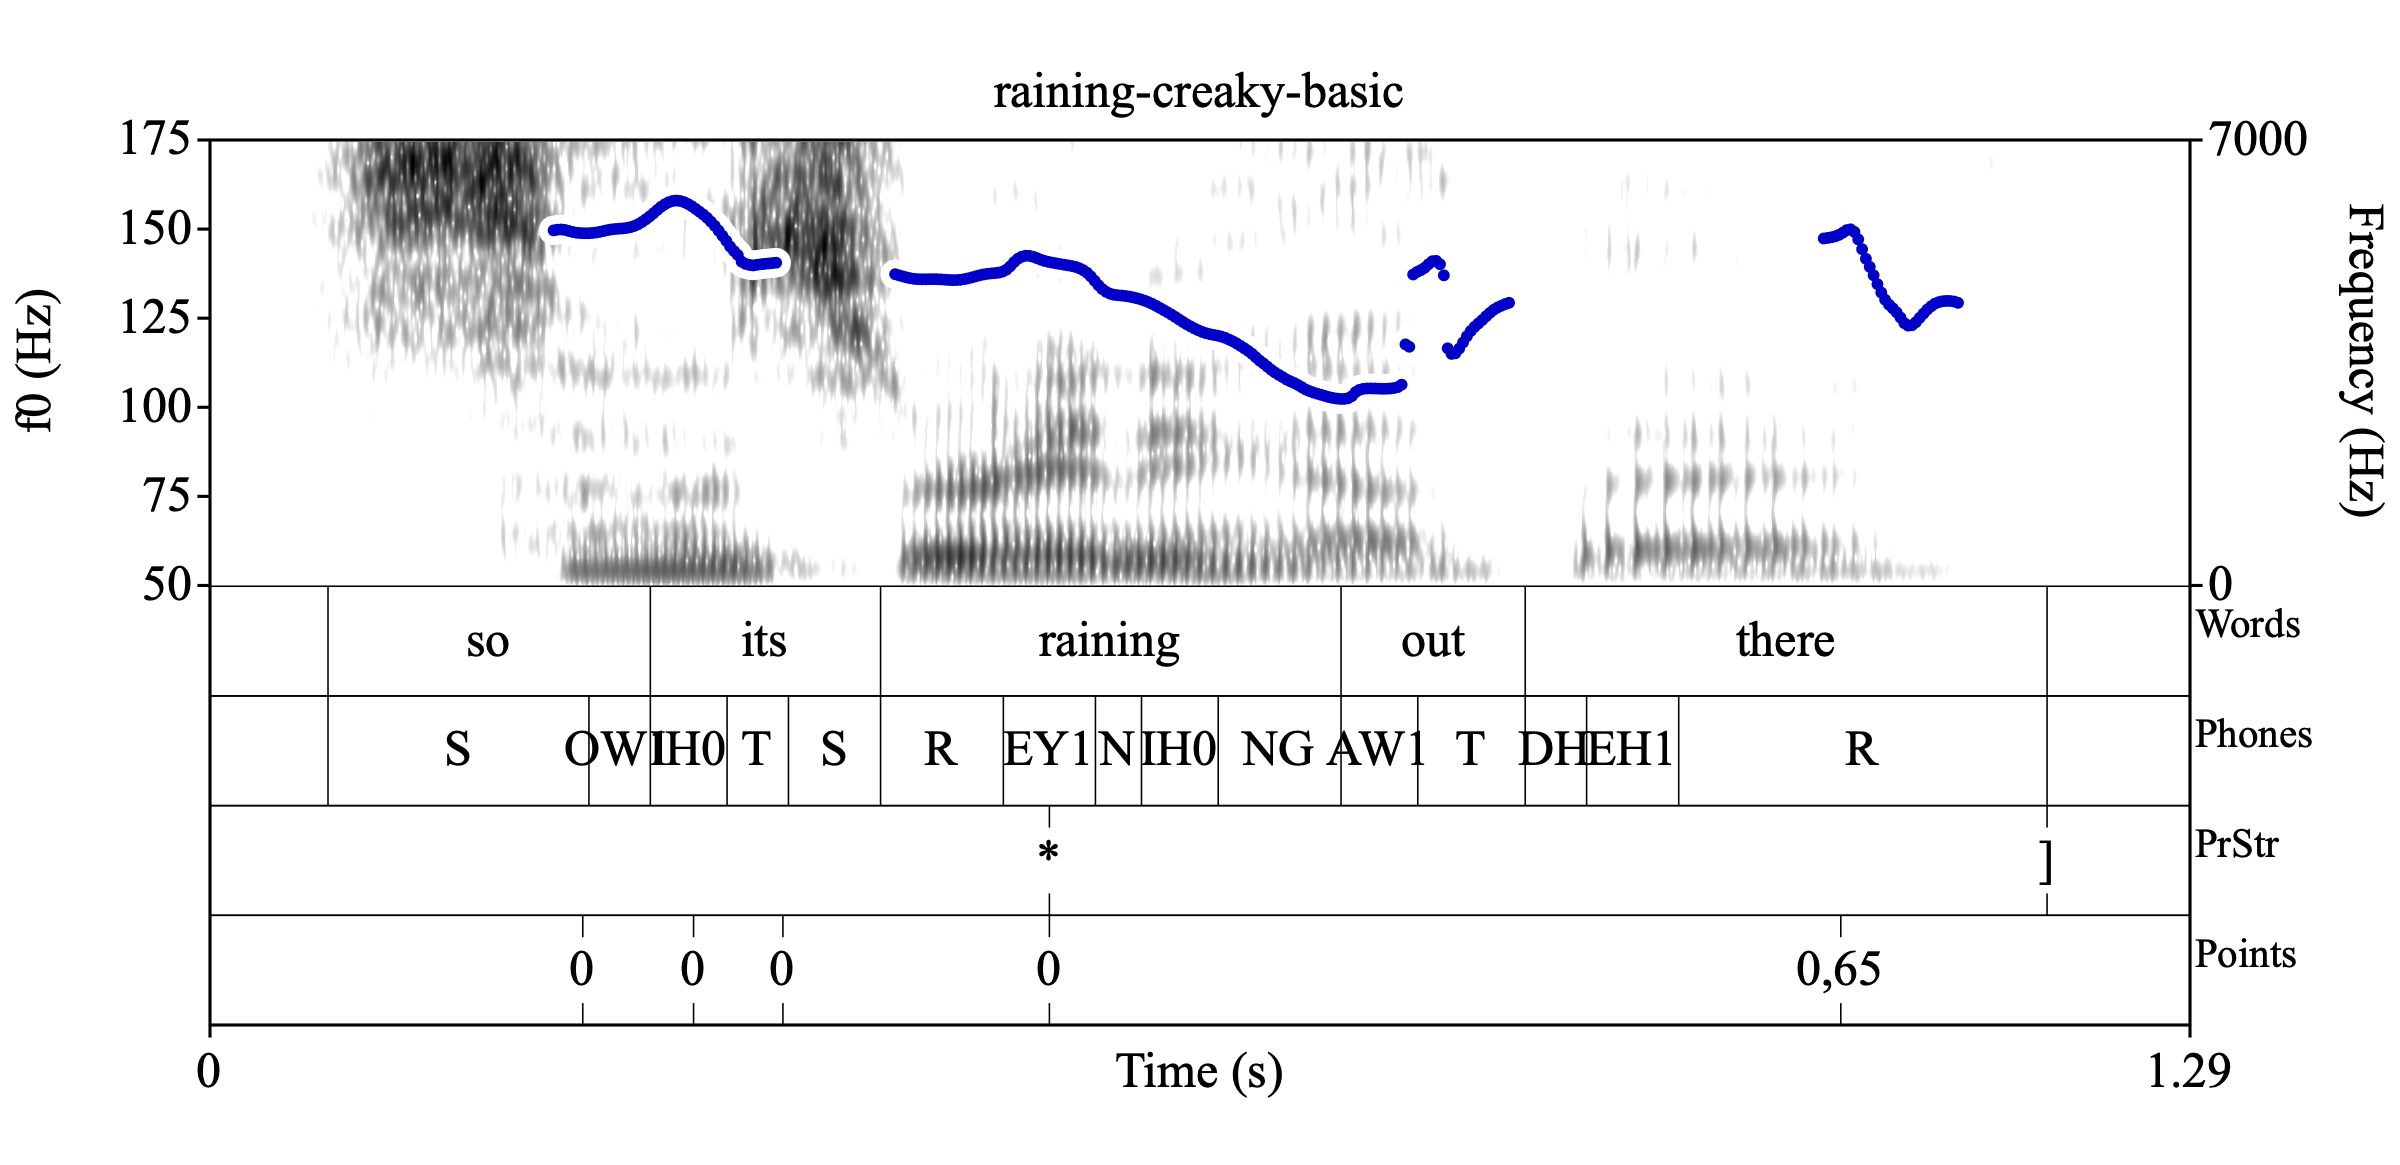
\includegraphics[width=.875\linewidth]{Points-raining-creaky-basic-comma.png}
%
\caption{\texttt{raining-creaky}, with the f0 override PoLaR labels.%
\label{fig:raining-creaky Points comma}%
\index{Annotated example, PrStr tier (basic)!raining-creaky}%
}
\end{figure}

Here, the labellers heard the pitch falling steadily from the stressed vowel of “\langtext{raining}” to the end of the utterance, and estimated that the pitch at the end point of the fall should be about 65Hz (arriving at this number using a methodology described below). Since the initial f0 contour is reliable in this example, the initial ‘\textlabel{0}’ labels don’t need the help of the comma override. A resynthesized straight line approximation of this pitch, that perceptually matches the original, verifies there is no turning point near “\langtext{out}” even though the original software-generated f0 track (above) suggests there might be. This straight line approximation is shown in Figure \ref{fig:raining-creaky Points basic resynth}.

\begin{figure}[H]
\centering
%
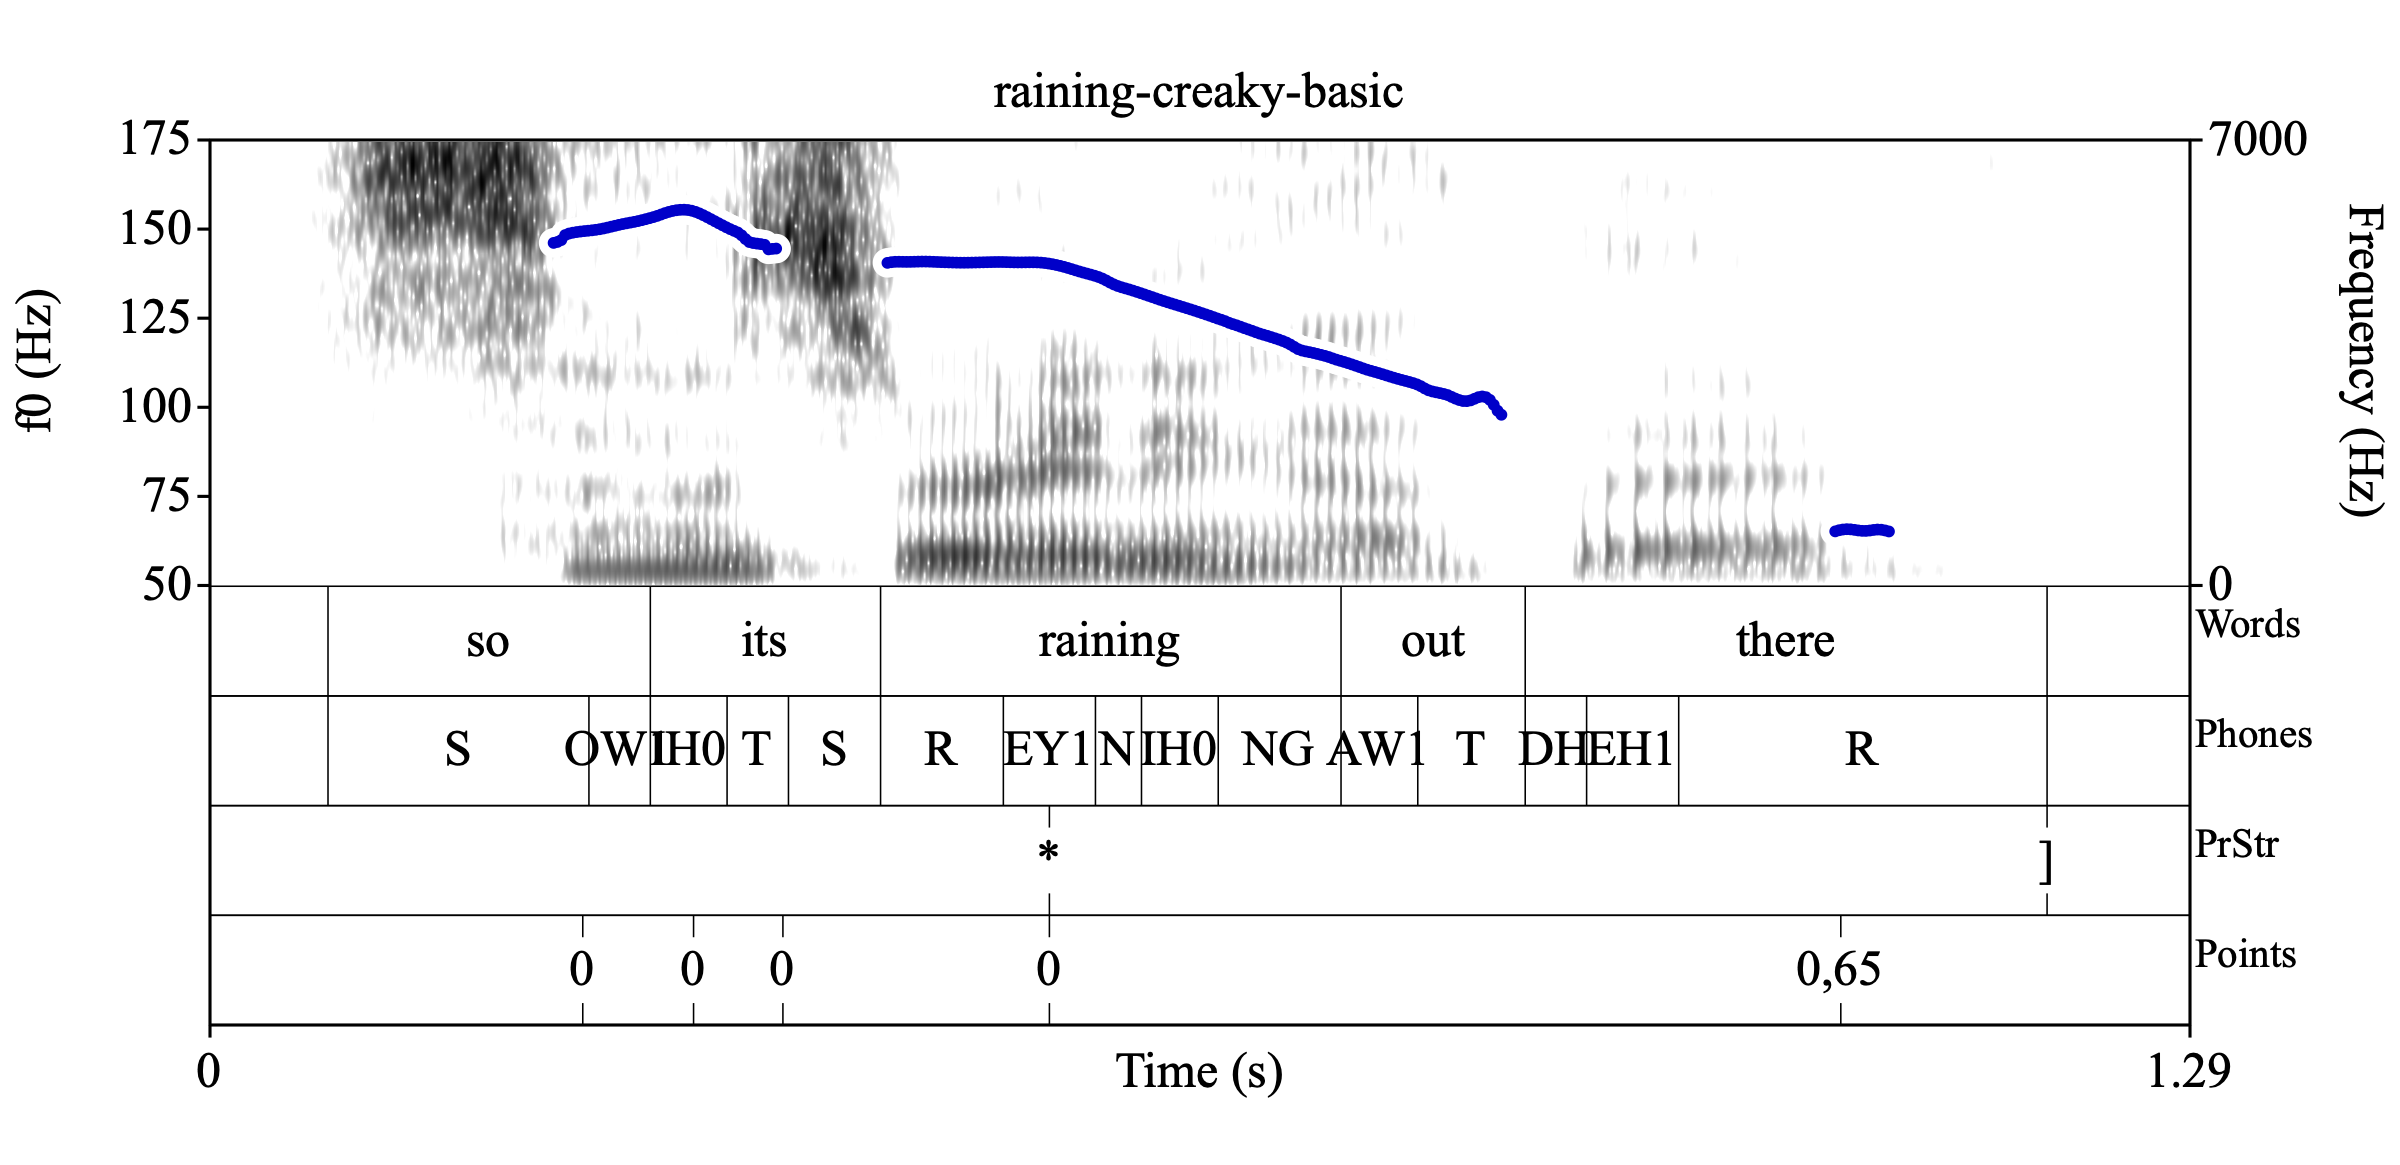
\includegraphics[width=.875\linewidth]{Points-raining-creaky-resynth-basic.png}
%
\caption{\texttt{raining-creaky-resynth} is a resynthesized straight-line approximation that is perceived as sounding intonationally the same as the original recording, \texttt{raining-creaky}.%
\label{fig:raining-creaky Points basic resynth}%
\index{Annotated example, Points tier (basic)!raining-creaky}%
}
\end{figure}

In cases like this (especially with creaky voice, which is so pervasive), labellers are encouraged to provide a guess at comma override values, resynthesize (with the Resynthesize Straight Line Approximation tool), and listen\slash compare the original and resynthesis. It may take several iterations of this, with different guesses at appropriate comma override values before the resynthesis sounds appropriately equivalent. (In cases where it is especially challenging or the labeller is uncertain about their comma overrides, they are encouraged to add a note to the Misc tier indicating this.) 

\paragraph{Pitch Override Points Example 2: End of an utterance\label{pitch-override-points-example-2}}

In a second case, the pitch tracking for the boundary-related tones is unreliable at best (in part because of non-modal phonation beginning in “\langtext{order}” and lasting through the end of “\langtext{again}”). Notice that though there are some valleys in “\langtext{of}” and the beginning of “\langtext{order}”, there are no perceptible falls in pitch there (as confirmed by the straight line approximations achieved through pitch resynthesis). The pitch flattens out during again, though there is a slight perceptible rise (this may have to do with the switch from creaky to breathy phonation); because the f0 tracking is unreliable, as is often the case at the ends of an utterance, the f0 values are hard-coded into the final two Points labels.

\begin{figure}[H]
\centering
%
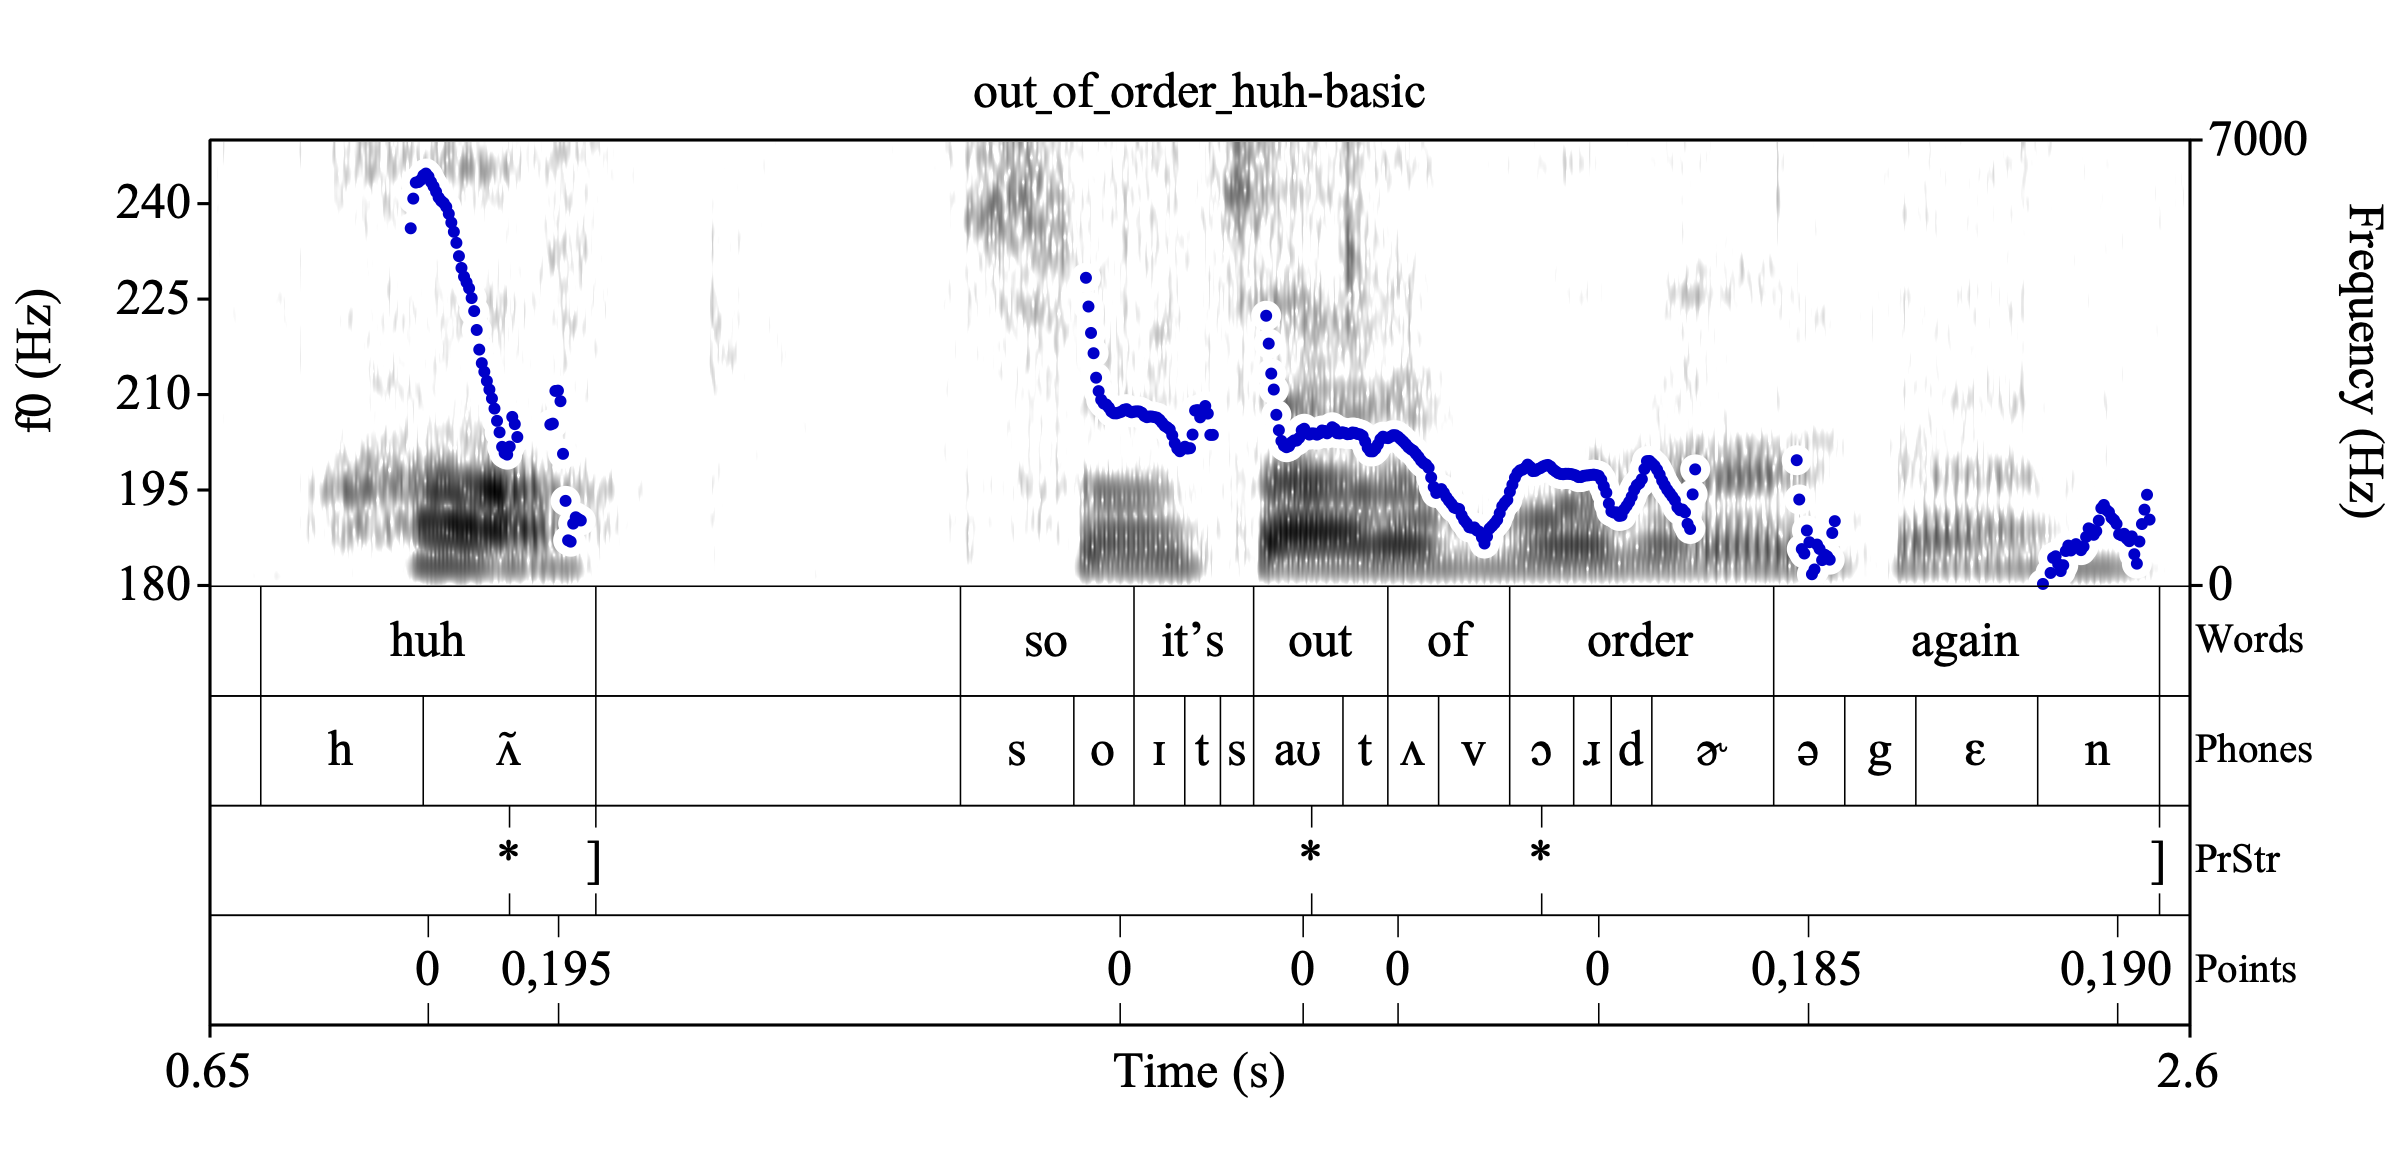
\includegraphics[width=.875\linewidth]{Points-out_of_order_huh-basic-comma.png}
%
\caption{\texttt{out\_of\_order\_huh}, with f0 override PoLaR labels.%
\label{fig:out_of_order_huh Points comma}%
\index{Annotated example, Points tier (basic)!out\_of\_order\_huh}%
}
\end{figure}

The f0 is unreliable in many locations. Using ‘\textlabel{0}’ (as we do for utterances at the beginning and end, respectively, of reliable f0) would not capture valuable information about the falls. 
%todo this is commented out… revisit this
%However, a labeller can approximate where in time the pitch reaches a particular frequency (based on auditory perception\slash visual cues from the pitch track), and the approximate value for that frequency (based on surrounding pitch tracking that appears to be reliable). PoLaR allows the annotator to include in the label what the pitch value “should be”, based on their intuitive\slash inferential abilities by appending a second label on the Points tier, using a comma delimiter followed by the f0 estimate. In the first label i
In this example, ‘\textlabel{0,195}’ indicates “This turning point is associated with a phrase boundary object time-aligned after this point, on the Prosodic Structure tier. The pitch value for this point should be 195Hz.” Thus the ‘\textlabel{,195}’ portion of the label overrides the f0-track (which lacks a pitch value at this point) and can be extracted as a replacement in later processing, such as comparing slopes of f0 movements.

This sort of “manual override” is not just for cases where f0 is absent but can be used for unreliable f0 as is the case with the final two turning points. The labeller judges that the last f0 interval is a mostly flat, rising from 185Hz to 190Hz, and uses ‘\textlabel{0,185}’ and ‘\textlabel{0,190}’ at each end to override whatever f0 value the pitch tracking software provides.

\paragraph{Pitch Override Points Example 3: Missing f0 values in voiceless speech\label{pitch-override-points-example-3}}

The case above is for a phrase end where pitch tracking is often unreliable, but this method of directly annotating pitch value approximations can be used for any Points tier object where the labeller is concerned that pitch tracking might not be reliable. Consider the example below, which contains three Points tier objects with manual-override pitch values:

\begin{figure}[H]
\centering
%
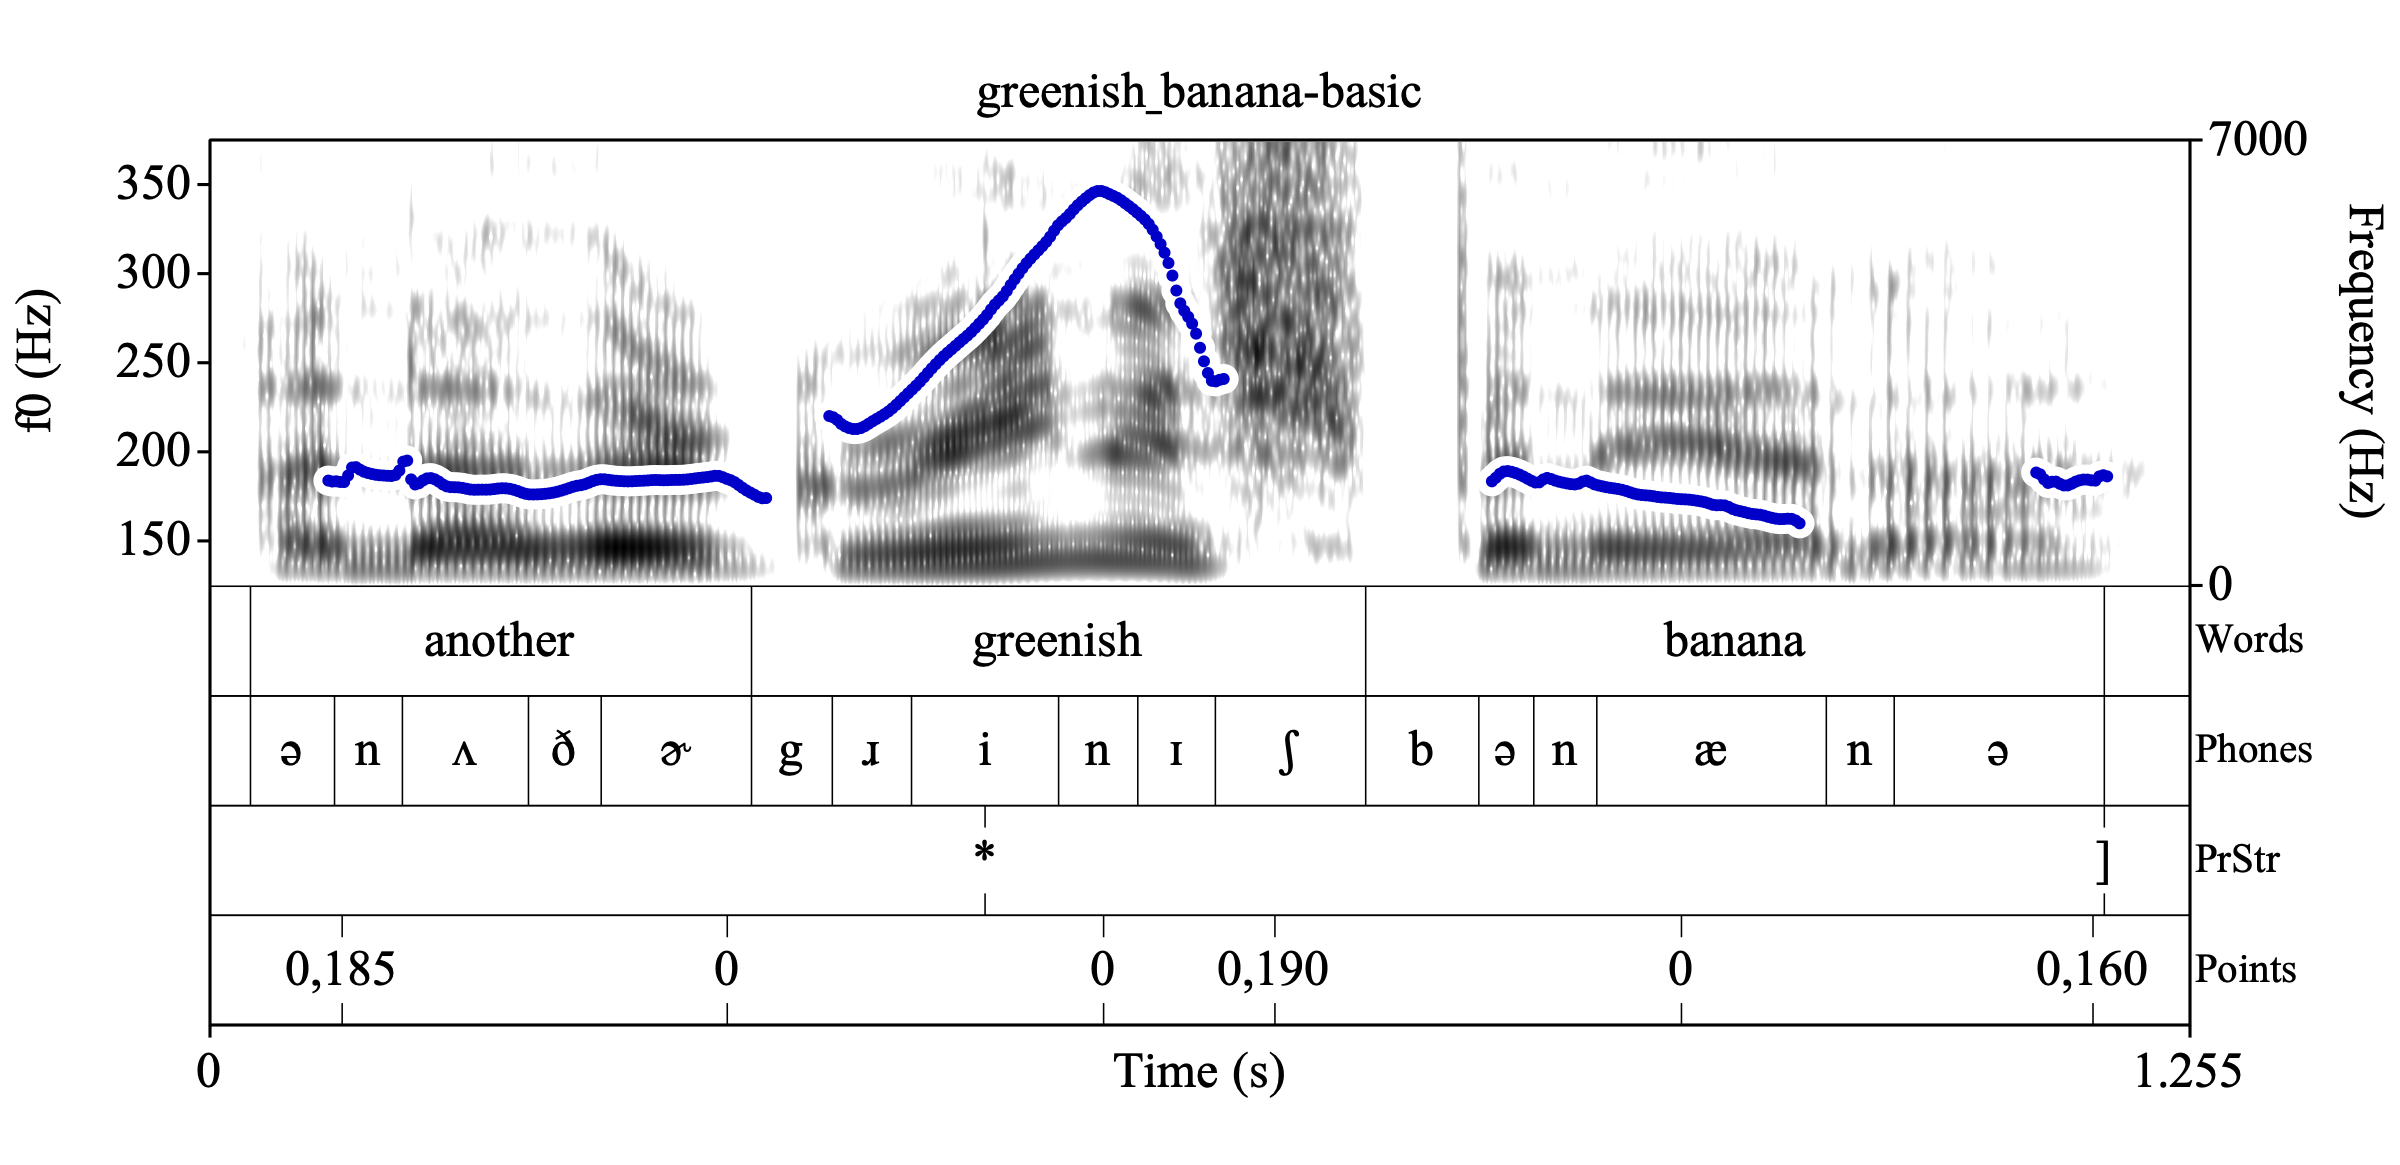
\includegraphics[width=.875\linewidth]{Points-greenish_banana-basic-comma.png}
%
\caption{\texttt{greenish\_banana}, with the f0 override PoLaR labels.%
\label{fig:greenish banana Points comma}%
\index{Annotated example, PrStr tier (basic)!greenish\_banana}%
}
\end{figure}

Let’s begin in the word “\langtext{greenish}”. Here the listener perceives a turning point in the middle of the voiceless [ʃ], and estimate its pitch value to be about 190Hz, given the slopes of the f0 track line segments that flank it. Additionally, the pitch is perceived to continuously fall during “\langtext{banana}”, so the final upward-inflected pitch at the end is perceived to be mis-tracked, and the labellers provide an inferred pitch value of 160Hz. Finally, the beginning of this utterance has an f0 at around 185Hz: the pitch tracking is a little jittery, so the labeller has appended the initial ‘\textlabel{0}’ label with ‘\textlabel{,185}’ so as to not have to worry about the software identifying an incorrect value for this turning point. Also note, again, the comma override is used to capture the final f0 in the utterance.

\paragraph{Pitch Override Points Example 4: Missing f0 during presumptive turning points\label{pitch-override-points-example-4}}

In this final example, we notice that the f0 tracking is interrupted during an interval of time at the end of the word \langtext{Stein’s}. A labeller can infer that an f0 peak might occur right during this interruption – visually, one could imagine that the pitch is rising to a peak that occurs where the two line segments would intersect, if they were lines instead of line segments. However, this inferred peak will require a comma override value, since Praat is not tracking any f0 during this time. The label ‘\textlabel{0,420}’ marks the inferred time-alignment and f0 value of this peak.


\begin{figure}[H]
\centering
%
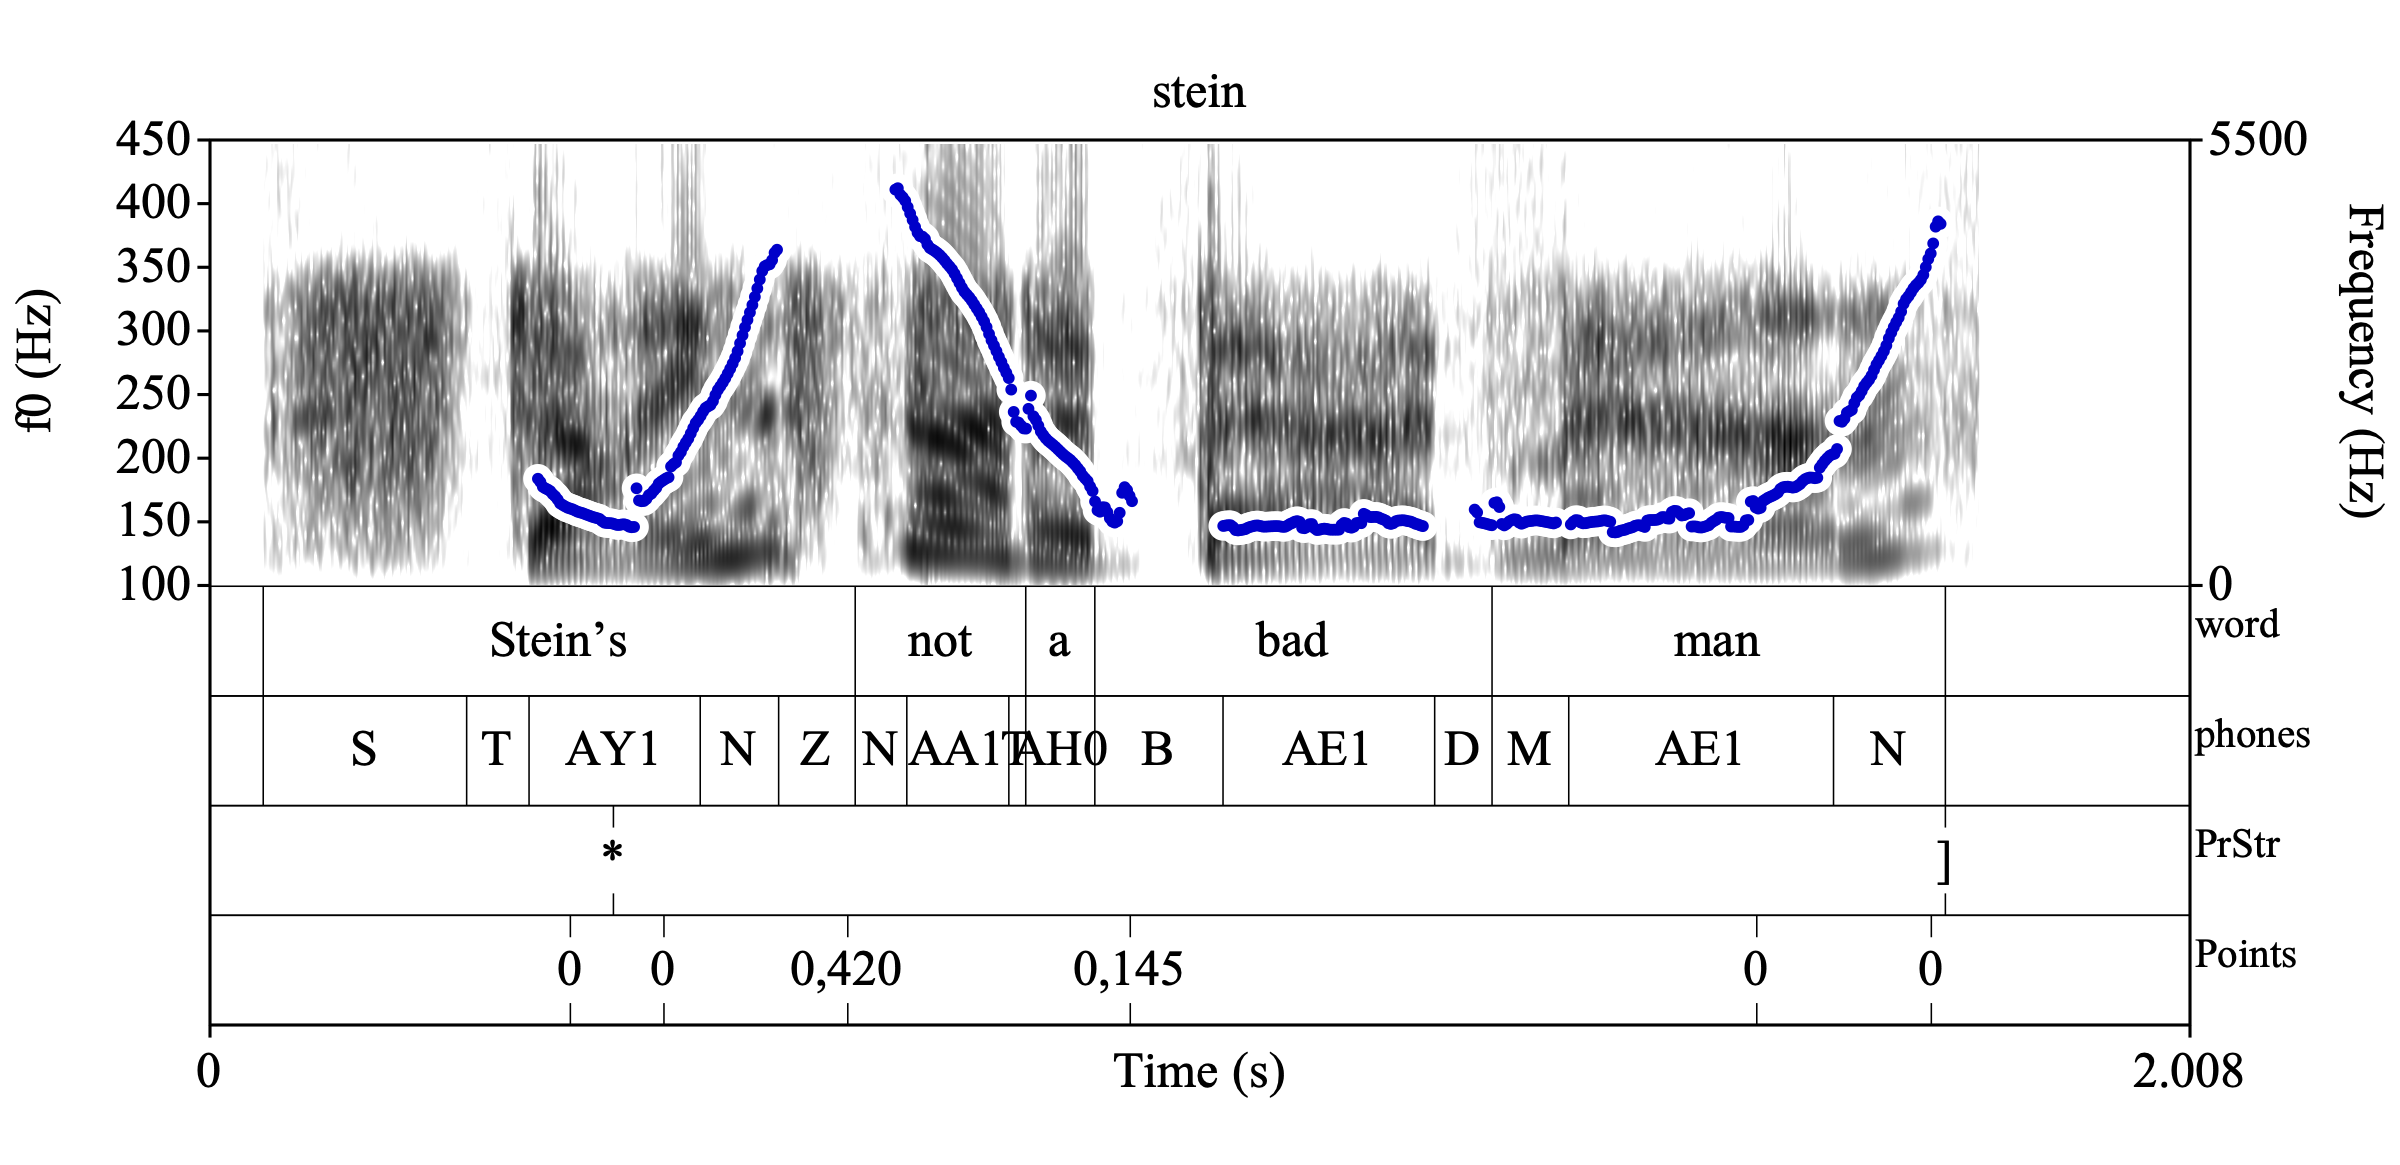
\includegraphics[width=.875\linewidth]{Points-stein-basic.png}
%
\caption{\texttt{stein}, with f0 override to label the “ghost” point at the presumptive peak.%
\label{fig:stein Points comma}%
\index{Annotated example, PrStr tier (basic)!stein}%
}
\end{figure}

The placement of the Points label (with the comma override) in the middle of this voiceless interval creates a resynthesized straight-line approximation that sounds perceptually identical, helping to justify the time-alignment and comma-override value for the ‘\textlabel{0,420}’ label.

\begin{figure}[H]
\centering
%
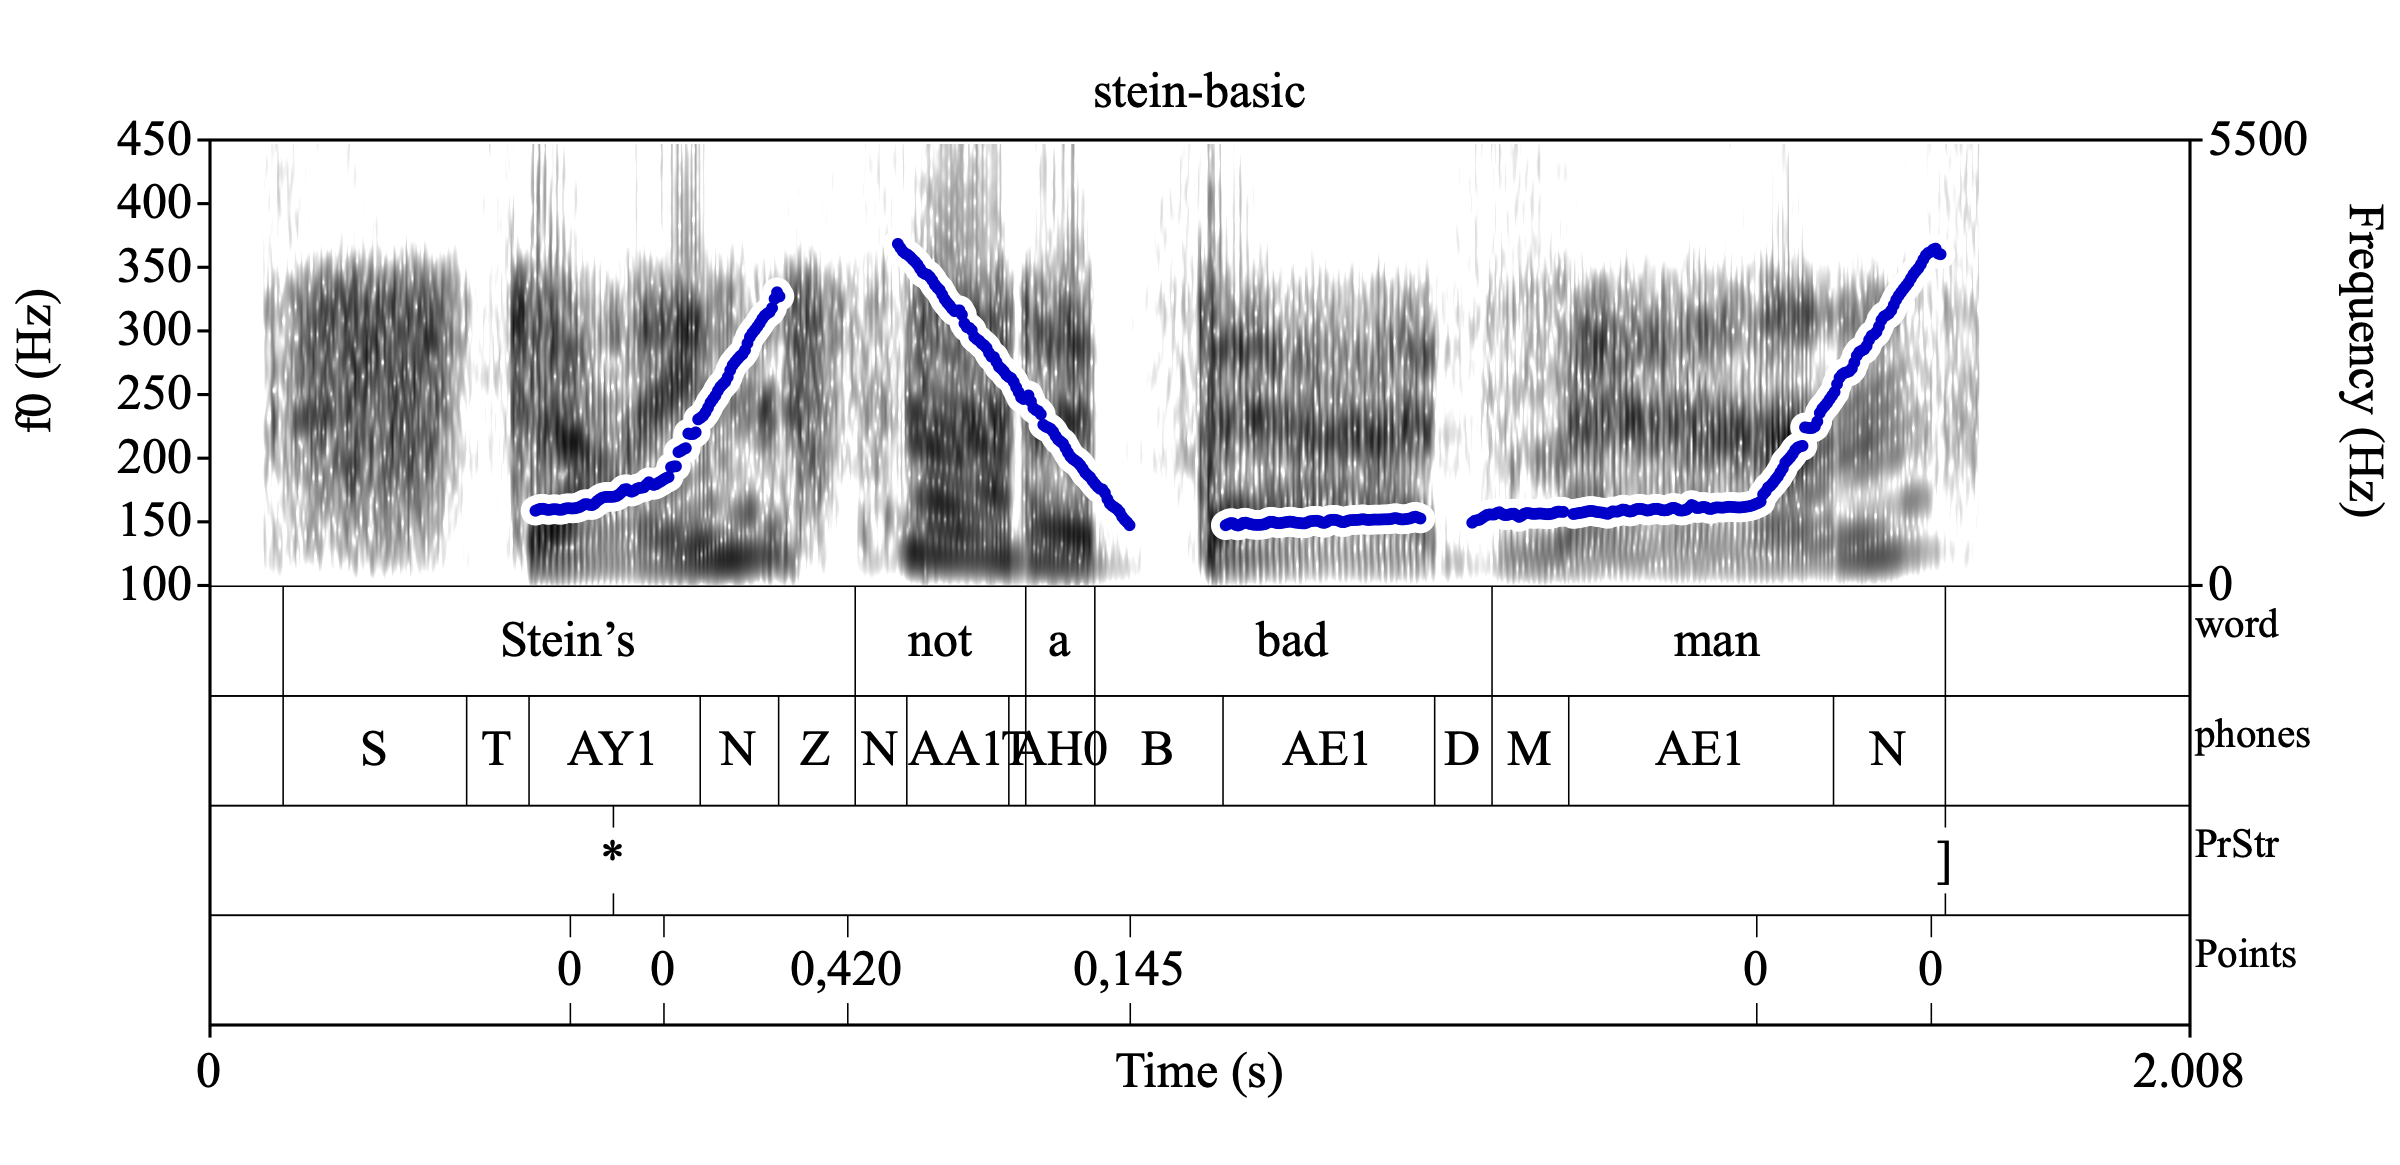
\includegraphics[width=.875\linewidth]{Points-stein-basic-resynth.png}
%
\caption{\texttt{stein}, with a straight line approximation resynthesis, on the basis of the “ghost” point peak.%
\label{fig:stein Points comma SLA}%
\index{Annotated example, PrStr tier (basic)!stein}%
}
\end{figure}


\subsubsection{Points labels summary}\label{sec:points-labels-summary}

To summarize, the three labels we have seen so far are described in Table \ref{Points basic labels}.

\begin{longtable}{cp{.8\linewidth}} \toprule \textbf{Label} & \textbf{Meaning} \tabularnewline
\midrule \endhead
\textlabel{0} & A turning point in the f0 contour (where line segments meet in a straight-line approximation of the pitch) \tabularnewline
\textlabel{?0} & Labeller is uncertain whether it is necessary to annotate a turning point in the f0 contour, even after exploring options with the straight line approximation resynthesis tool \tabularnewline
\textlabel{0,X} & An f0 turning point whose pitch value is approximately X (a labeller’s approximation of the f0 when the software-based f0 tracking is unreliable) \tabularnewline
\bottomrule 
\caption{The Basic labels for the Points tier (for English).%
\label{Points basic labels}%
}
\end{longtable}


\subsection{Ranges Tier}\label{sec:ranges}
%My first and main issue regards the Pitch Ranges tier. To summarize, a) on the x-axis (temporal dimension), labellers identify the scope of such a pitch range for different portions of an utterance. Importantly, the scope of a given pitch range is independent of phrase breaks and may be assigned to any part of an utterance. Also, b) on the y-axis, annotators identify the f0 range (min / max) of a portion of an utterance and label the min and max on a tier. Min and max do not necessary refer to the actual minimum and maximum f0 value observed in the signal, but are values that the labellers determine as minimum and maximum for a particular speaker [BTA: or context!].
% Regarding a), allowing misaligned f0 ranges and phrases is difficult both from a theoretical and practical point of view and – in my opinion – not sufficiently motivated in the manuscript. From a theoretical point of view, I am not convinced how – within one and the same phrase – speakers may employ different ranges. The authors themselves argue that phrase breaks may trigger a change in the f0 range (p. 106); I am not sure which kind of processes would trigger a change in f0 range within one and the same word. From a methodological perspective, this assumption or possibility in PoLaR might lead to inconsistencies in labelling. That is, I am concerned about both the validity of the range annotation and its reliability. In fact, even though I am quite experienced in annotation, I would not have placed all f0 ranges as done by the authors, e.g., on p. 46, 106, 108, 109. I thus wonder how reliable the positioning of these range spaces is, which in turn, has implications for the pitch levels, as they are informed by the pitch ranges.
	%> response: address this by raising the question of "what are Ranges supposed to do?" and then describe how there are researcher-/project-level choices that can be made to further guide choices
	%> labellers are encouraged to *consider* whether there is a new Ranges interval, according to…
		%> phrase boundary (new phrase <-/-> new Range, but the two do have high co-incidence)
		%> downstep / upstep (phonologically conditioned changes)
			%> this can occur word-medially!
		%> voice quality shifts (modal -> falsetto; extended creak -> modal)
%With respect to b) (y-axis), I also have a methodological and a theoretical concern: Methodologically, I think that inferring speakers’ actual highs and lows requires intensive experience and such inferences are particularly prone for interrater variability. More importantly, assigning pitch levels based on the min/max of the f0 range represents a normalization that gets rid of the actual f0 values – which in some cases might be relevant indeed. I totally see that in some cases, e.g., the cases of range compression (p. 104) it is straightforward to apply such a normalization, but there might be cases, e.g., in different registers such as infant-directed speech, in which information of the actual values of pitch targets is important (e.g., when voices go into falsetto). Taken together, the Ranges Tier in my view allows for too many “degrees of freedom” (Roettger, 2019) for labellers. This, in turn, may decrease reproducibility and reliability, which brings me to my second point.
	%> response: there is variation, of course, but again – what matters is what the researcher **aims to do** with them. anecdotally, we have found that there are differences, of course, in labels here but they are *surprisingly* more consistent than might be expected
	%> response: again, this is a question of what we ought to do with Ranges annotations.
		% should we compare annotations across labs? only with care!
		% should we be able to compare ranges within labs? ABSOLUTELY!
		% does this f0 normalization (ranges->levels) erase variation? kind of, but on purpose, and in a way that actually allows labellers to keep track of the shifts (e.g., going into falsetto is tracked by Ranges in a way that is completely untracked in other annotation systems)
The Range Domains Tier is an interval tier, in which the pitch range is annotated over a portion of speech. In essence, a shift in “Range” is a shift in what counts as low and/or high pitch.

Accordingly, the key function of the Ranges tier is to define the local lows and highs that intonation alternates between: changing ranges allows you to compare two different pitch values and say they’re both "highs" even if one is much higher\slash lower than the other. Before we discuss how this tier is labelled, some pre-discussion is necessary about “pitch range”.

We assume that there are three usages of the term “pitch range”.\footnote{For a more in depth discussion and overview of pitch range, as well as the related terms “pitch span” and “pitch register,” see \citealt{gussenhoven04}, Chapter 5, especially pp. 77-80.} These three usages are: (i) the “physiological pitch range” of the speaker, covering frequencies from all the pitches that their vocal anatomy allows them to produce, (ii) the “comfortably implementable pitch range” of the speaker, covering a speaker’s comfortable low pitch to their comfortable high pitch, and (iii) the “local pitch range” within a particular utterance, which operationally demarcates where “low” targets and “high” targets go, for this particular portion of speech.

For example, consider the following example from NPR radio (\href{https://www.npr.org/sections/goatsandsoda/2018/05/11/603315432/the-best-mothers-day-gift-get-mom-out-of-the-box}{source}):

\begin{figure}[H]
\centering
%
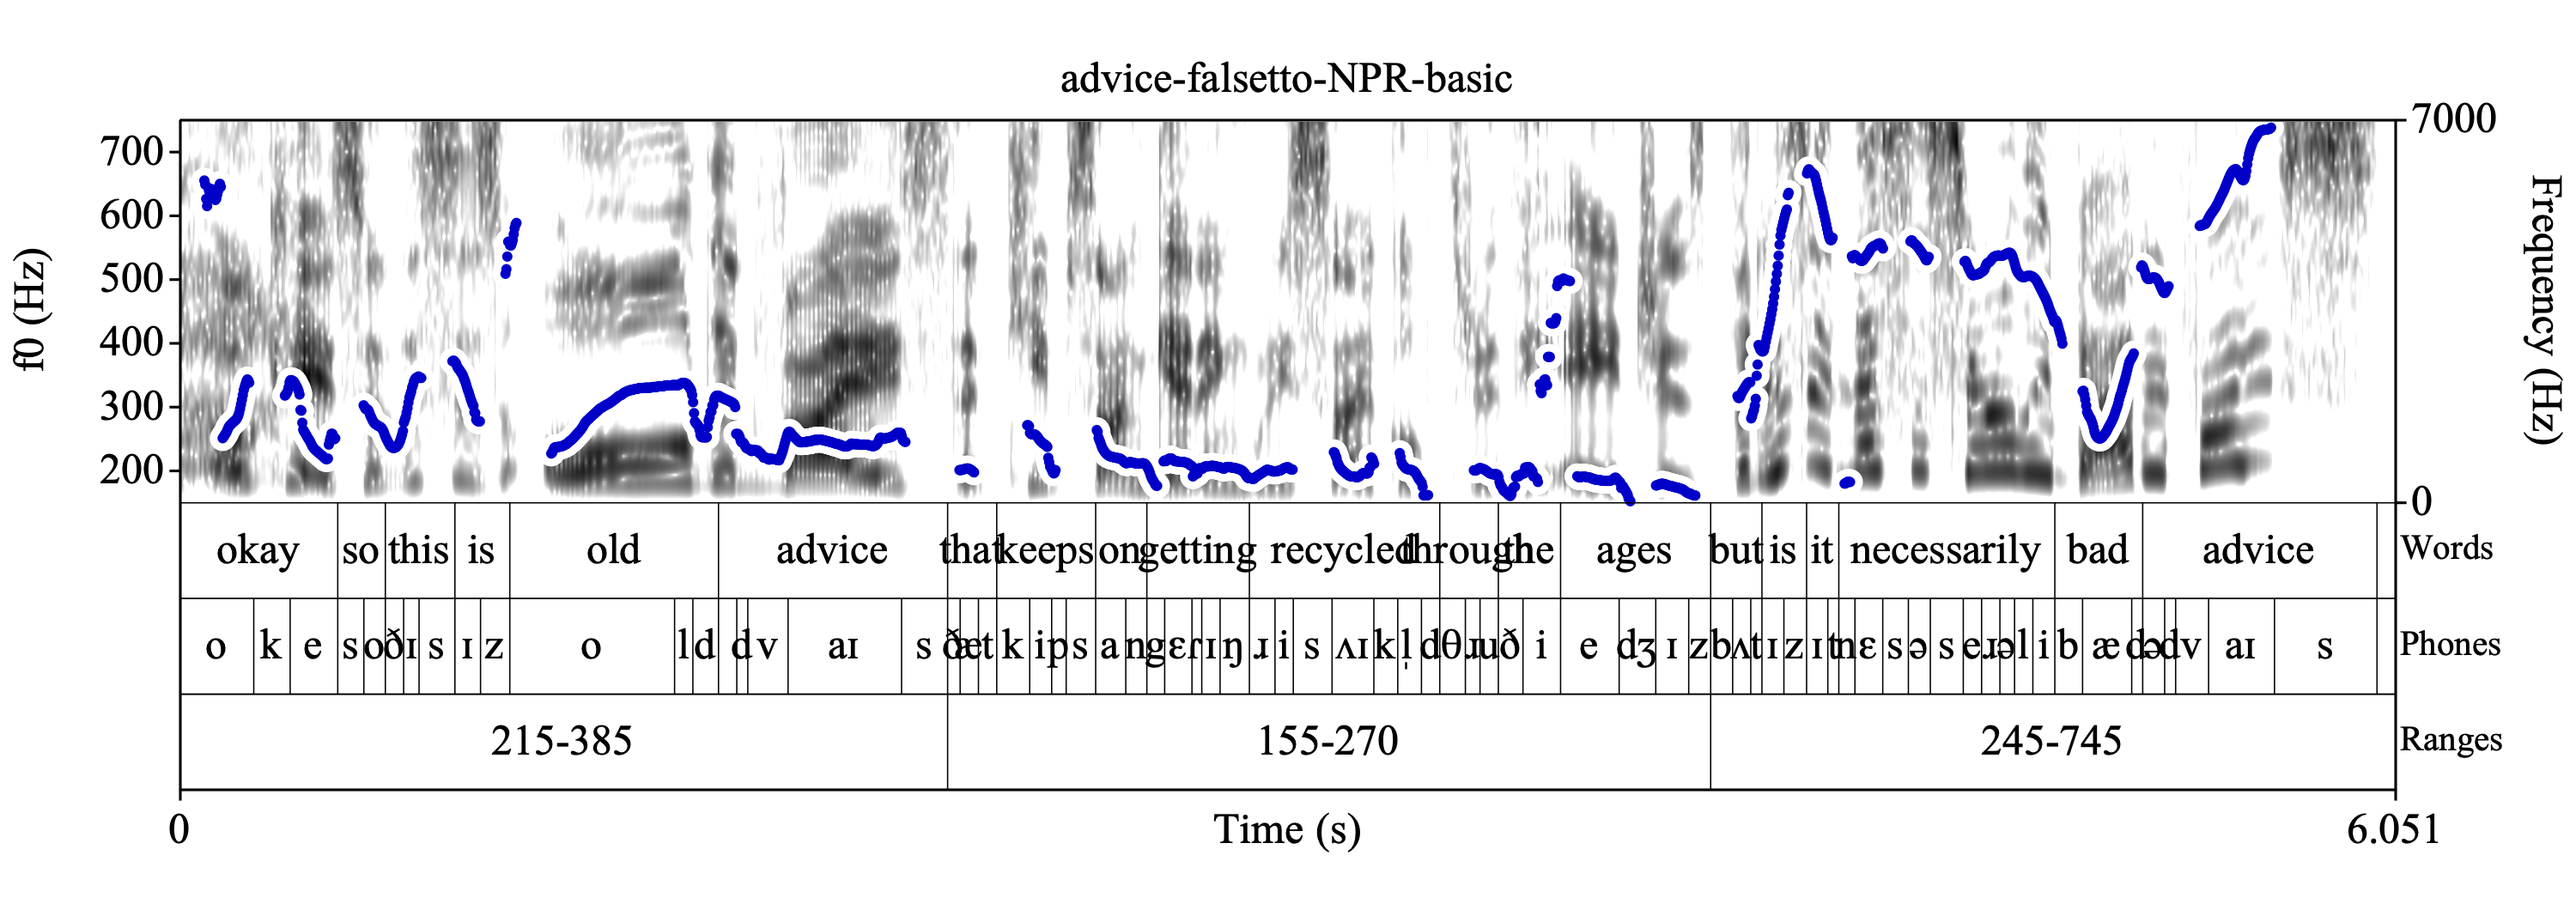
\includegraphics[width=\linewidth]{Ranges-advice-falsetto-basic-all-3-ranges.png}
%
\caption{An example of a long utterance with three pitch range intervals.%
\label{fig:advice-falsetto Ranges basic}%
\index{Annotated example, Ranges tier (basic)!advice-falsetto}%
}
\end{figure}

Let us discuss how this example embodies all three types of pitch ranges. Here, the speaker must have a \uline{physiological pitch range} that allows at least a range of 150Hz-750Hz (though likely it is bigger). In the latter part of the recording, the speaker is using a falsetto voice, and the end of the utterance could be analyzed as “super high” in that high falsetto range. Depending on the speaker, this extreme falsetto high pitch can reasonably be considered outside of their \uline{comfortably implementable pitch range}.

Viewing the entire utterance as a whole, one can perceive it as having three different \uline{local pitch ranges}, \textbf{each of which is labelled as an interval on the “Ranges” tier}. Consider the high and low pitch in “\langtext{okay so this is old advice}” compared to the highs and lows in “\langtext{but is it necessarily bad advice}”. Although the highs and lows in “\langtext{okay\ldots advice}” are much lower than in “\langtext{but is it\ldots advice}”, on their own, they can be perceived as \uline{locally} high (even though, e.g., “\langtext{okay}” is much lower than the later highs) and low. Similarly, these highs and lows are also different from the highs and lows in “\langtext{that keeps on getting recycled through the ages}”.

Labelled Range boundaries do not always co-occur with prosodic phrase boundaries. A local pitch range interval may span multiple prosodic phrases. An example of this can be found for an early part of the advice-falsetto-NPR example:

\begin{figure}[H]
\centering
%
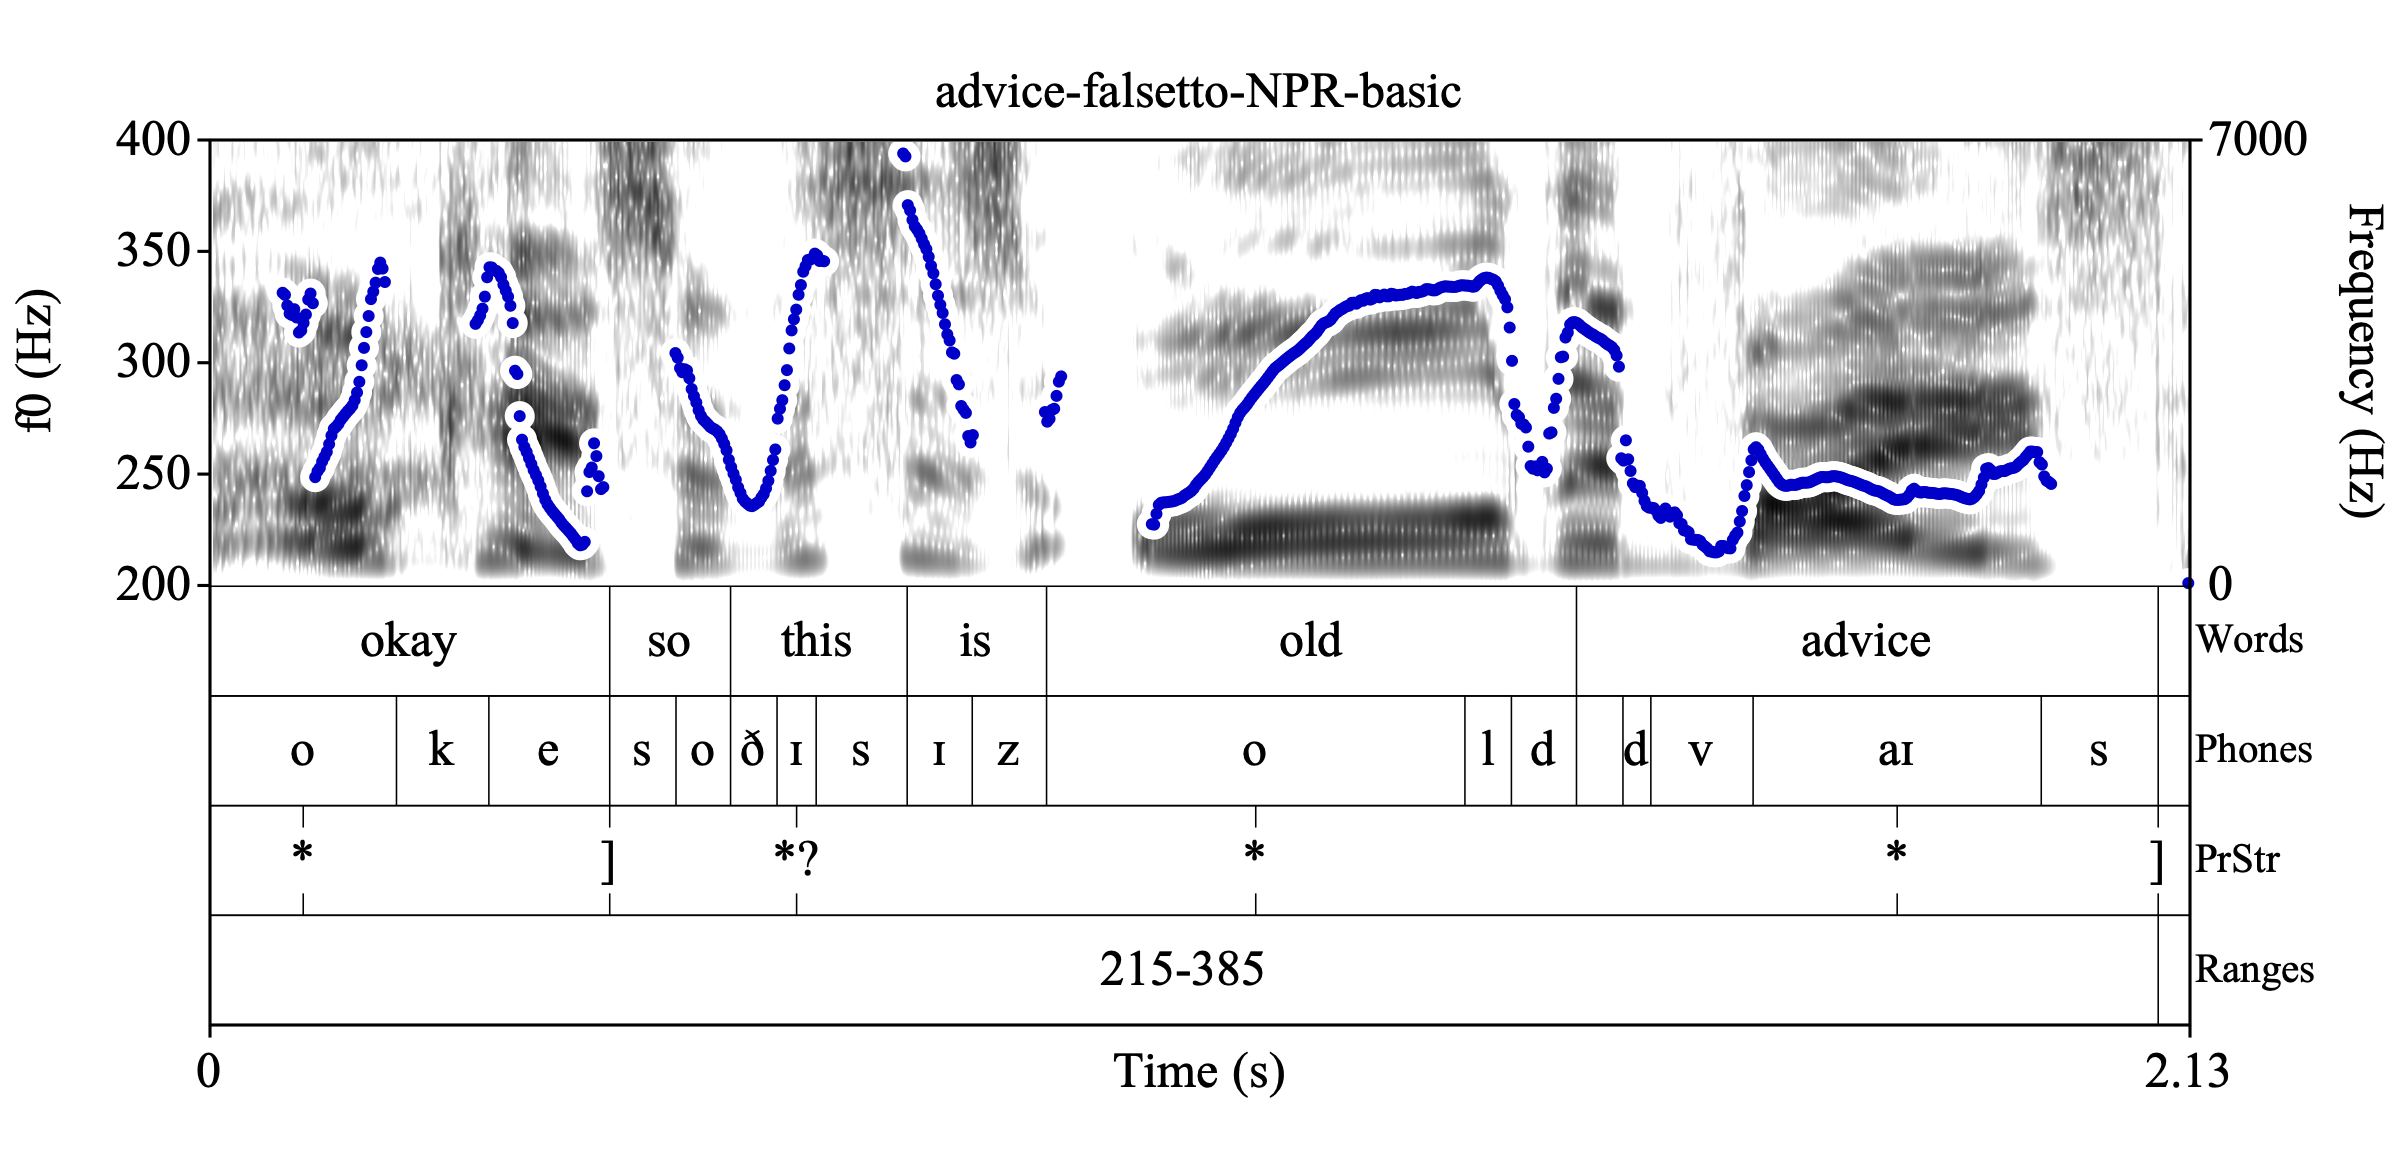
\includegraphics[width=.875\linewidth]{Ranges-advice-falsetto-basic-first-range.png}
%
\caption{Two prosodic phrases (PrStr annotation) and one local pitch range (Ranges annotation).%
\label{fig:advice-falsetto PrStr Ranges basic}%
\index{Annotated example, Ranges tier (basic)!advice-falsetto}%
\index{Annotated example, PrStr tier (basic)!advice-falsetto}%
}
\end{figure}

Conversely, a single phrase as labelled in the PrStr tier may contain multiple ranges, a topic which will be addressed in more detail in section \ref{sec:ranges-advanced} of chapter \ref{ch:advanced}.

Because Ranges constituents need not have a one-to-one correspondence to prosodic phrases on the PrStr tier, the Ranges tier labeller need not even have PrStr tier labels to do their work, and the Ranges tier can be labelled independently of all other tiers. If the PrStr tier is in place, when a new prosodic phrase begins, it’s not necessarily the case that there will be a new local pitch range. At the same time, it seems that in some cases a new local pitch range may serve as a cue that a new prosodic phrase has begun (cf. \citealt{brugos15}, \citealt{brugos-18}, and \citealt{kim20}). In this way, a labeller may find it useful to consider whether a new range interval is necessary when there is a new phrase, but they do not necessarily need to attend to conventional prosodic phrase boundaries when doing this labelling.

Labelling the Ranges tier requires labellers to consciously engage in thinking about concepts that may be unfamiliar (e.g., identifying locally “high” pitch, even where the speaker is speaking in a low and narrow pitch range). Not many individuals are practiced in engaging their intuition in this way, and new labellers may find it challenging. Ultimately, however, these intuitions will be necessary for relating the Points tier to more categorical labels of pitch “height” (e.g., values 1-5 on the Levels tier, or “high”\slash ”low” even more generally). More on this will be addressed in section \ref{sec:ranges-advanced} of chapter \ref{ch:advanced}.

\subsubsection{Getting started with the annotation of Ranges:}\label{sec:getting-started-with-the-annotation-of-ranges}

Each stretch of PoLaR-labelled speech must contain minimally one pitch range, i.e., an f0 floor and an f0 ceiling must be noted for that stretch of speech, such that the f0 minimum and maximum for that stretch are captured within that range. As a rule of thumb when starting out labelling, the labeller may find it useful to consider the pitch range to every speech interval bounded by strong temporal cues to phrase boundaries, such as silent pauses or breaths. (Bear in mind that such a group may well contain more than one range, and or that sequential stretches of speech separated by a pause or other boundary cues may be contained within a single range.)

If the labeller has access to PrStr labels, they may find it useful to consider ranges with respect to phrases as delimited by the \textlabel{]} label. At the same time, domains for ranges need not be determined by phrases labelled in the PrStr tier. Even a short stretch of speech may well turn out to contain local pitch range changes, as described in the Advanced labels chapter (Ch.\ref{ch:advanced}). Conversely, sequential phrases may be perceived as part of the same range. Ranges may to some extent suggest groupings among phrases, such as those labelled with \textlabel{]} in the PrStr tier. In this way, PoLaR Ranges annotation gives the labeller the means to capture more complicated relations where phrase boundaries (as annotated via the PrStr tier) and ranges can be somewhat independent: ranges can be annotated delinked from other boundary cues.

\subsubsection{Local Pitch Ranges: Typical Cases}\label{sec:local-pitch-ranges-typical-cases}

The most straightforward case will be an isolated short phrase, with a small number of events labelled in the Points and PrStr tiers, and a single labelled pitch Range. However, in dynamic speech, utterances of more than a few words are likely to consist of more than one range interval.

For each (part of an) utterance, a speaker (often unconsciously) picks out a portion of their physiological pitch range, the lower part of which corresponds to frequencies for their (locally defined) lows, and the higher part of which corresponds to frequencies for their (locally defined) highs. In an ideal case, the intonational contour for an utterance will produce measurable f0 such that the minimum f0 is at (or around) the minimum of the local pitch range, and the maximum f0 is at (or around) the maximum of the local pitch range. Thus, if the f0 tracking (modulo any tracking errors) identifies the lowest f0 in an interval of time as 112.4Hz and the highest f0 in that same interval as 273.2Hz, the labeller can assume that these measurements reflect the local pitch range that the speaker is employing.

At the same time, the labeller should be a little cautious, and give a little wiggle room from the measured f0 min\slash max (rounding up or down to a number ending in 5 or 0, typically by at least 1 or 2 Hz, and often by a few more), since precise numbers are influenced by a number of factors, including software settings. Thus, a measured f0 range of 112.4Hz to 273.2Hz should have the min rounded down and max rounded up, and then be annotated as an interval in the Ranges tier with a label like ‘\textlabel{110-280}’. In other words, \textbf{in the typical case, (rounded) measures of local f0 min and local f0 max can be used to determine the label for a Ranges interval}. (This is the default guidance; more complex cases will be discussed here and in section \ref{sec:ranges-advanced} of Ch.\ref{ch:advanced}.)

Figure \ref{fig:amelia-knew2 Ranges basic} shows an example of a file annotated with the Ranges tier. Here, the minimum f0 is 114.7 Hz (in the [u] of “\langtext{minimum}”), and the maximum f0 is 248.3 Hz in the [l] of Amelia. The labeller has rounded down to a range minimum of 110 Hz and rounded up to a range maximum of 250 Hz.

\begin{figure}[H]
\centering
%
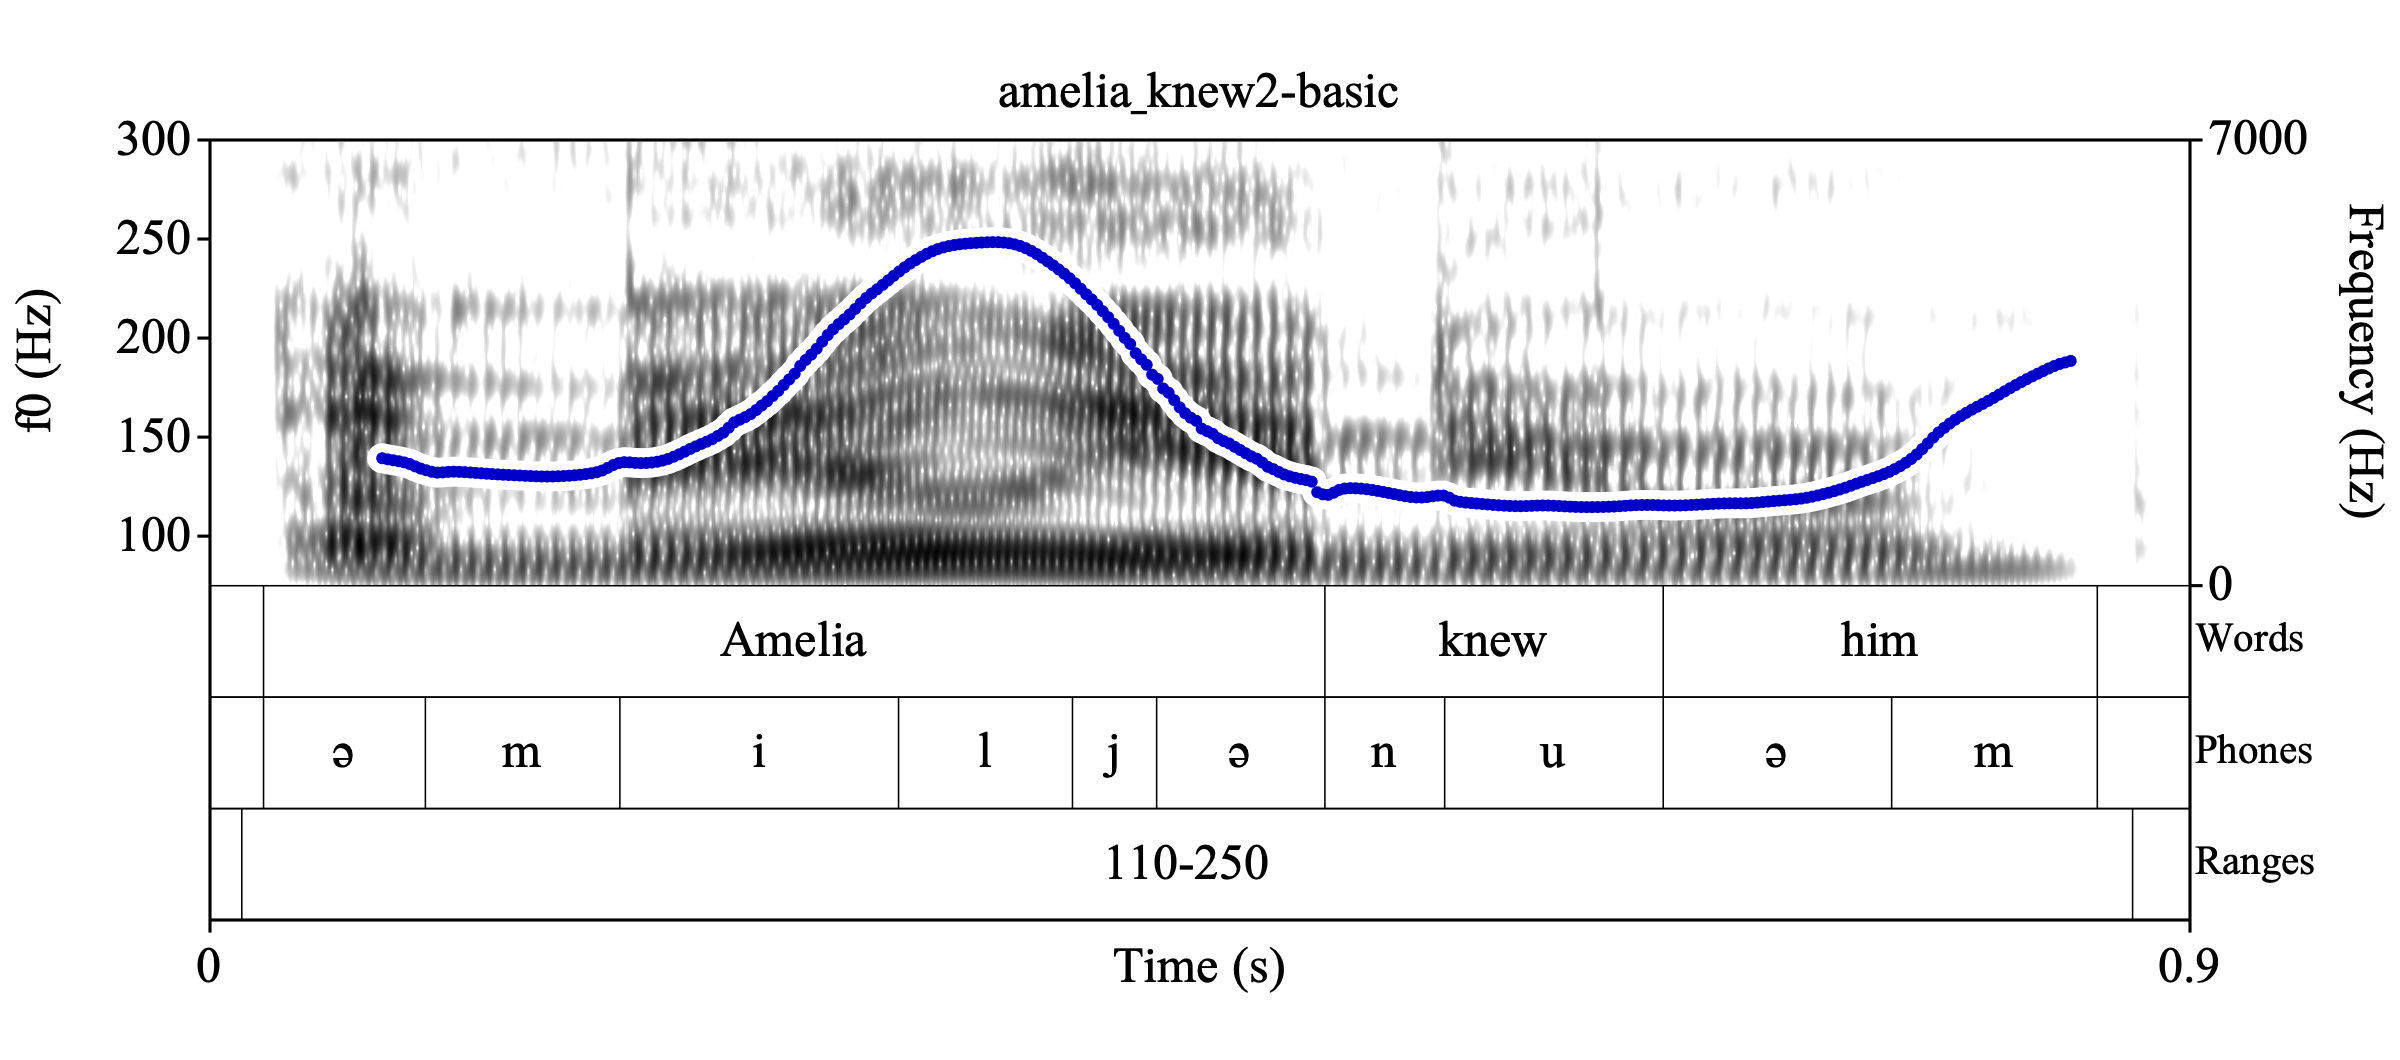
\includegraphics[width=.875\linewidth]{Ranges-amelia_knew2-basic.png}
%
\caption{An example of a short utterance with single pitch range interval, and clear pitch tracking.%
\label{fig:amelia-knew2 Ranges basic}%
\index{Annotated example, Ranges tier (basic)!amelia-knew2}%
}
\end{figure}

\begin{figure}[H]
\centering
%
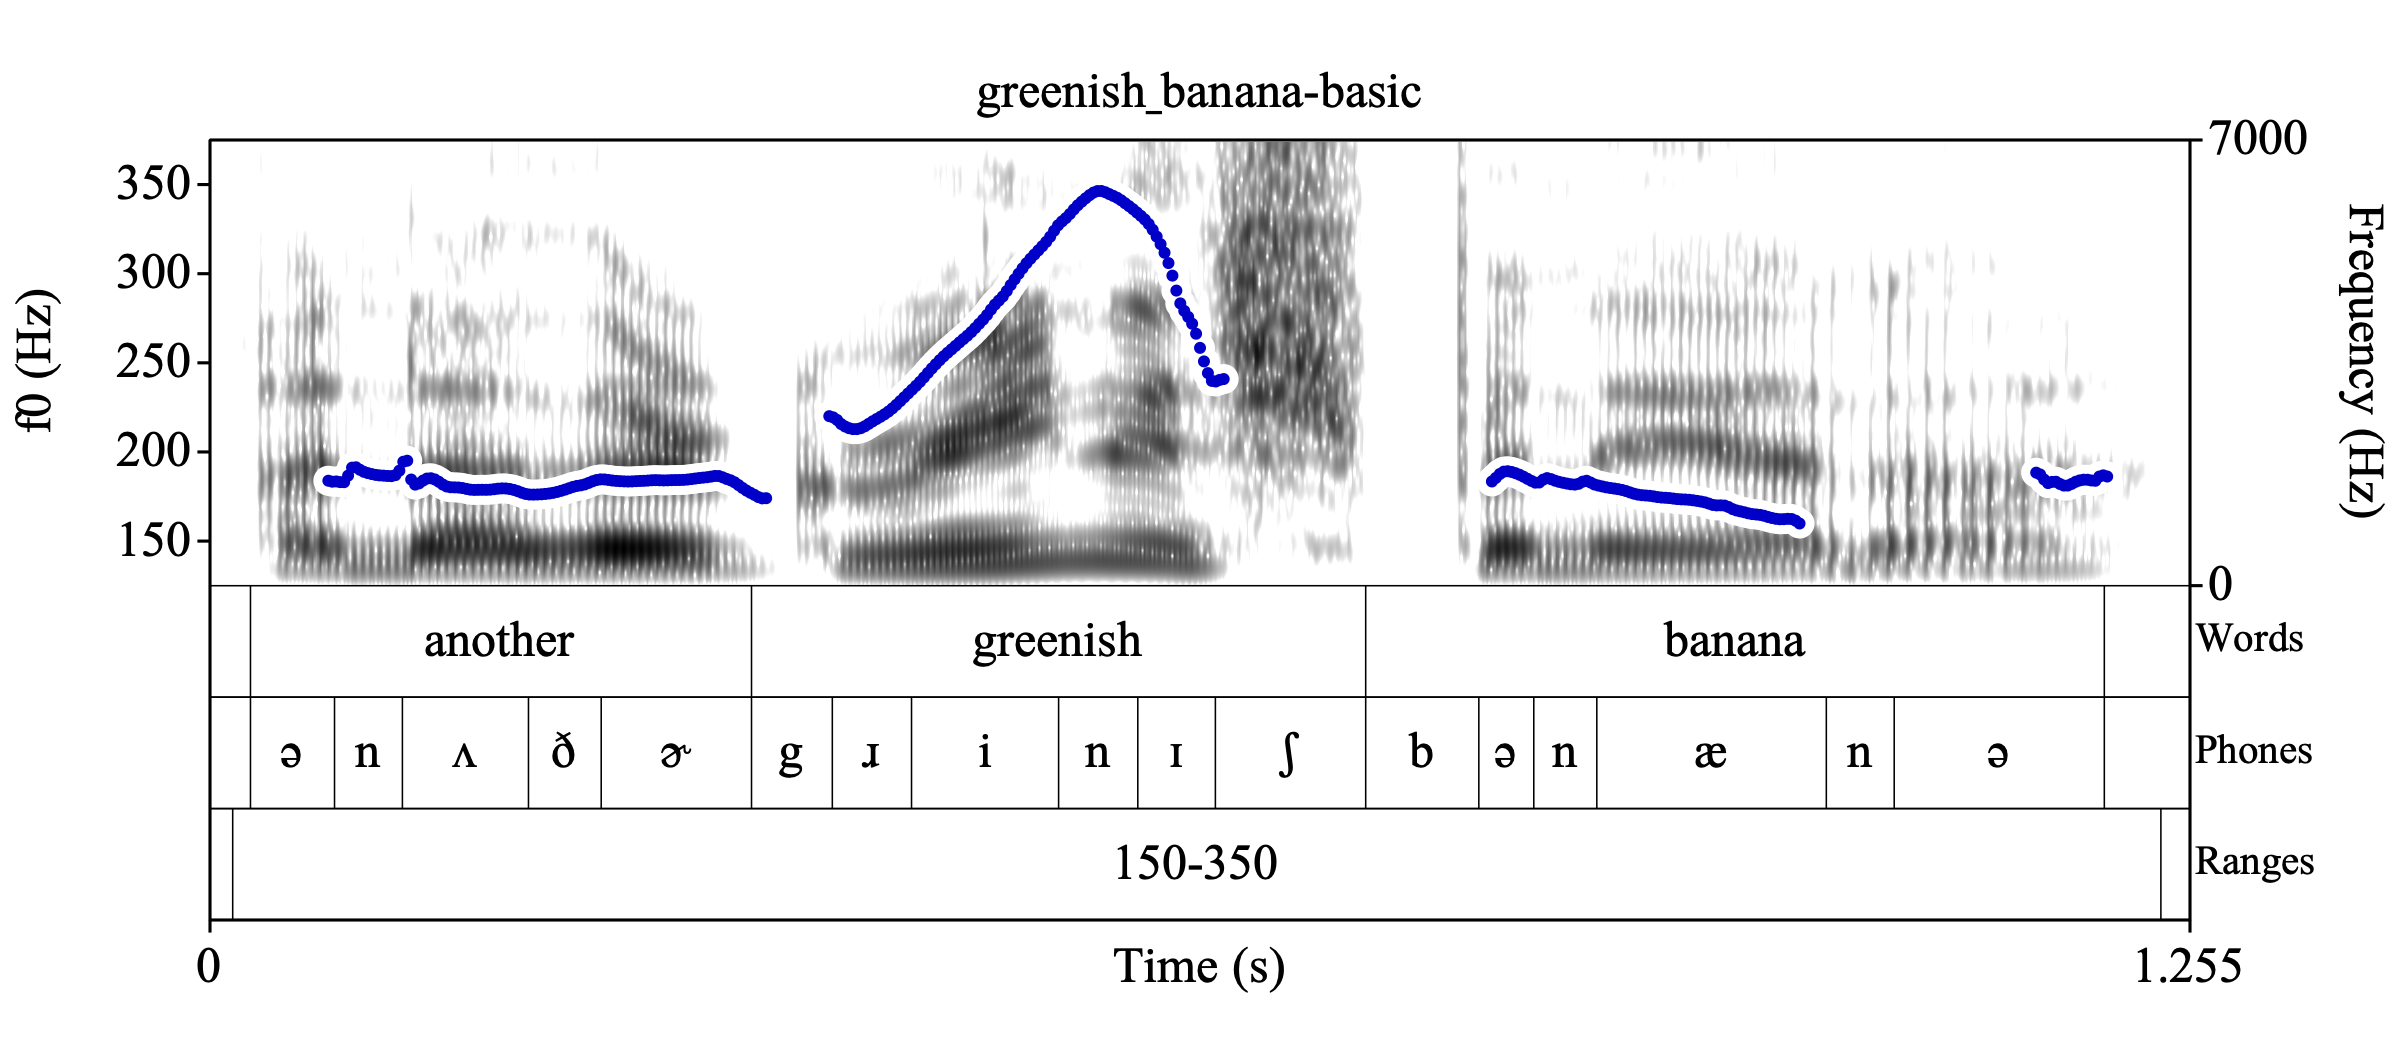
\includegraphics[width=.875\linewidth]{Ranges-greenish_banana-basic.png}
%
\caption[An example of a short utterance with single pitch range interval.]{An example of a short utterance with single pitch range interval, and a region of unreliable pitch tracking at the bottom of the speaker’s range.%
\label{fig:greenish-banana Ranges basic}%
\index{Annotated example, Ranges tier (basic)!greenish-banana}%
}
\end{figure}

Unlike in the example in Fig. \ref{fig:amelia-knew2 Ranges basic}, which shows a smooth pitch track, this example in Fig. \ref{fig:greenish-banana Ranges basic} shows pitch tracking unreliability where the speaker has produced creaky voice at the end of the utterance. In this case, the lowest reliable f0 is in the [æ] of banana, at 162 Hz. The labeller has chosen to round the bottom of the pitch range a bit lower, using 150 Hz. (The maximum of 345 Hz takes place during a region of reliable pitch tracking, and the labeller has rounded up to 350 Hz.) Pitch tracking errors at the end of phrases are very common, especially when the pitch is low and/or the speaker ends up creaking. The labeller should use their best estimate of how low the perceived f0 goes. 

The next example in Figure \ref{fig:no_cigar Ranges basic} (\texttt{no\_cigar}) shows a short utterance with two ranges, and the example following in Figure \ref{fig:tomorrow_morning Ranges basic} (\texttt{tomorrow\_morning}) shows another short utterance, this one with one range.


\begin{figure}[H]
\centering
%
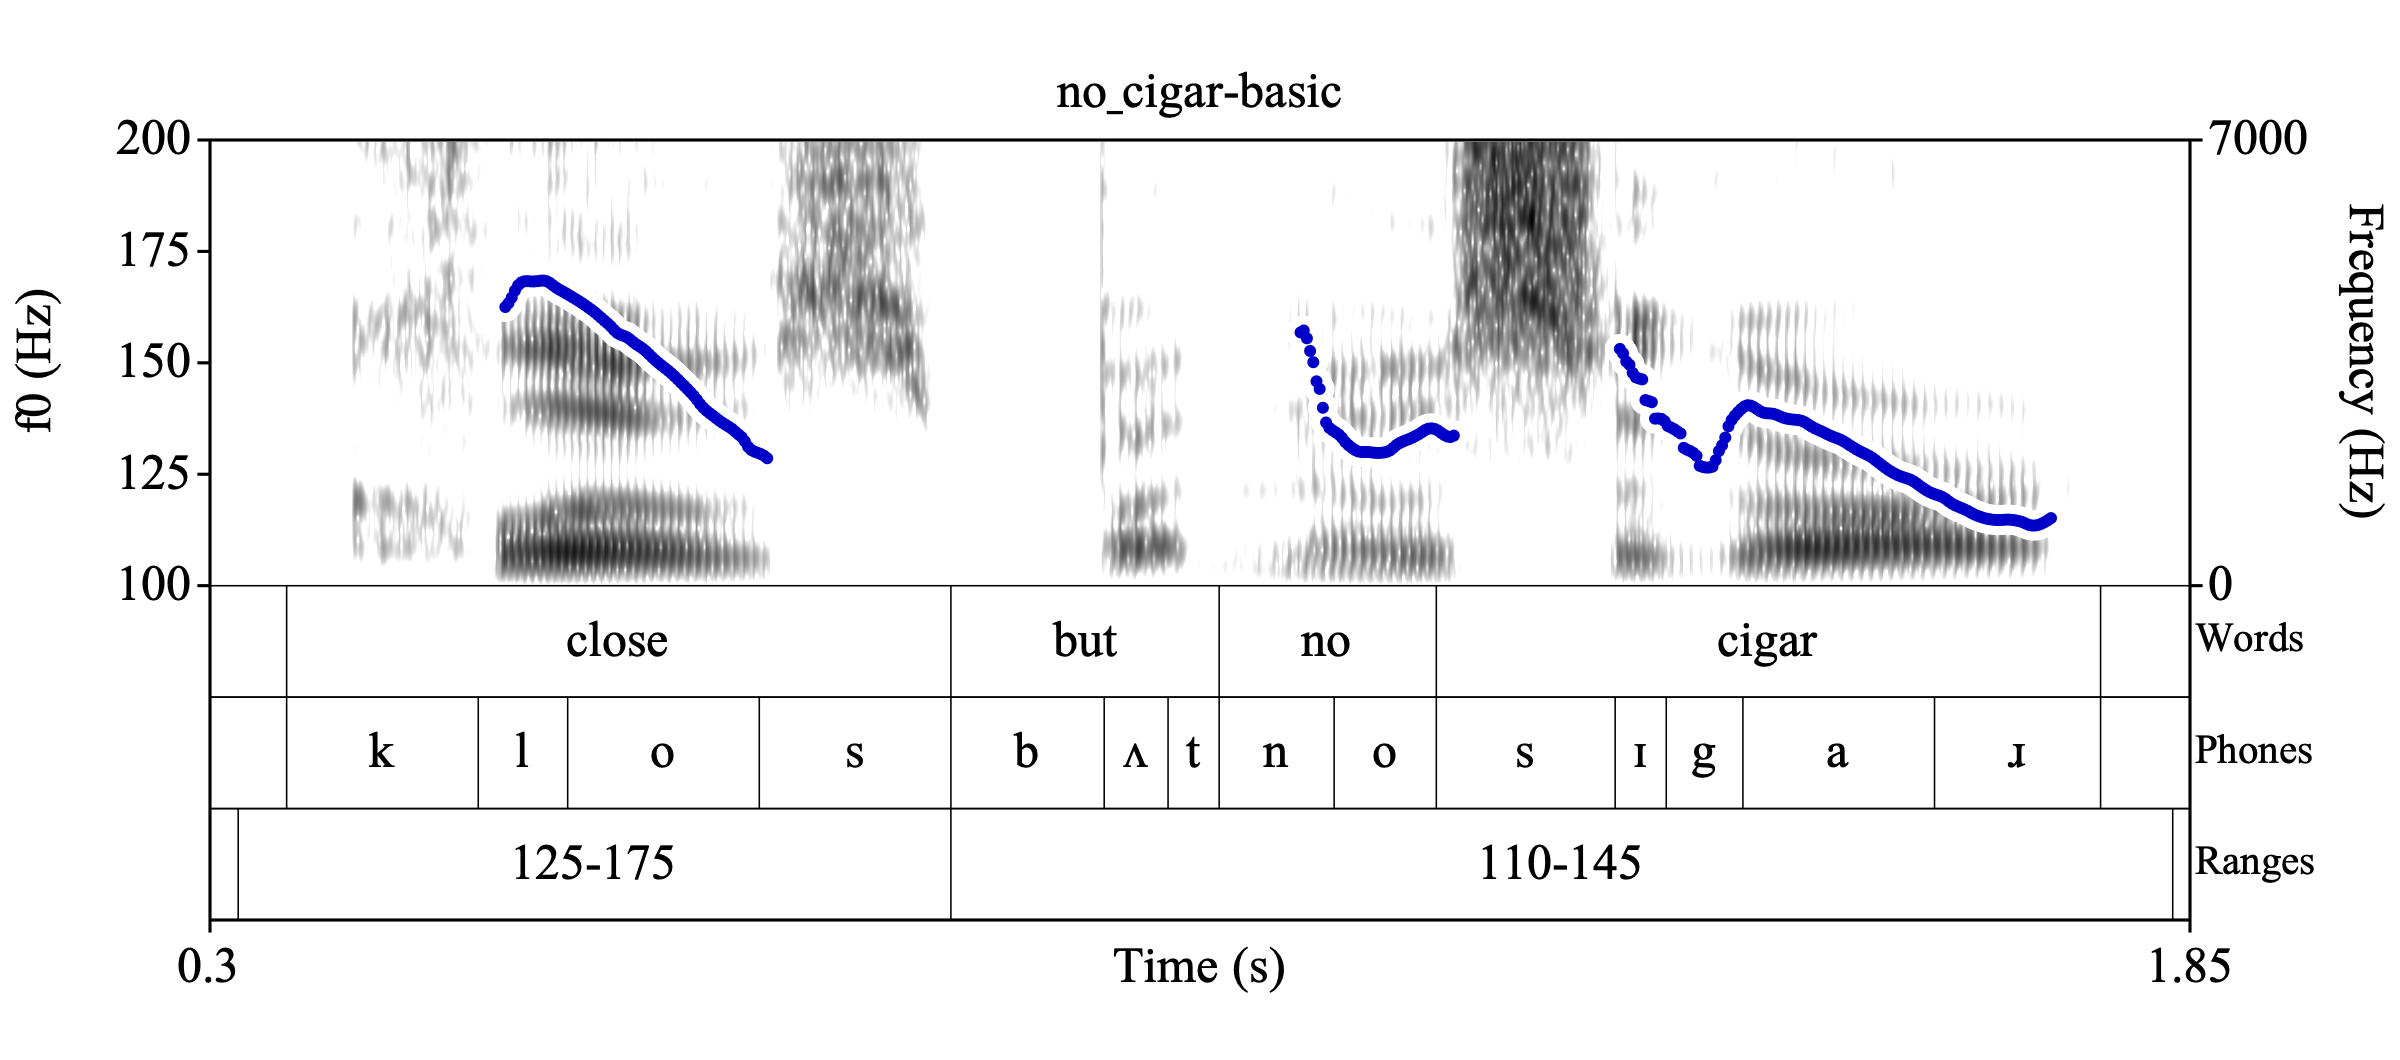
\includegraphics[width=.875\linewidth]{Ranges-no_cigar-basic.png}
%
\caption{This is an example of a short utterance with two ranges.%
\label{fig:no_cigar Ranges basic}%
\index{Annotated example, Ranges tier (basic)!no\_cigar}%
}
\end{figure}


\begin{figure}[H]
\centering
%
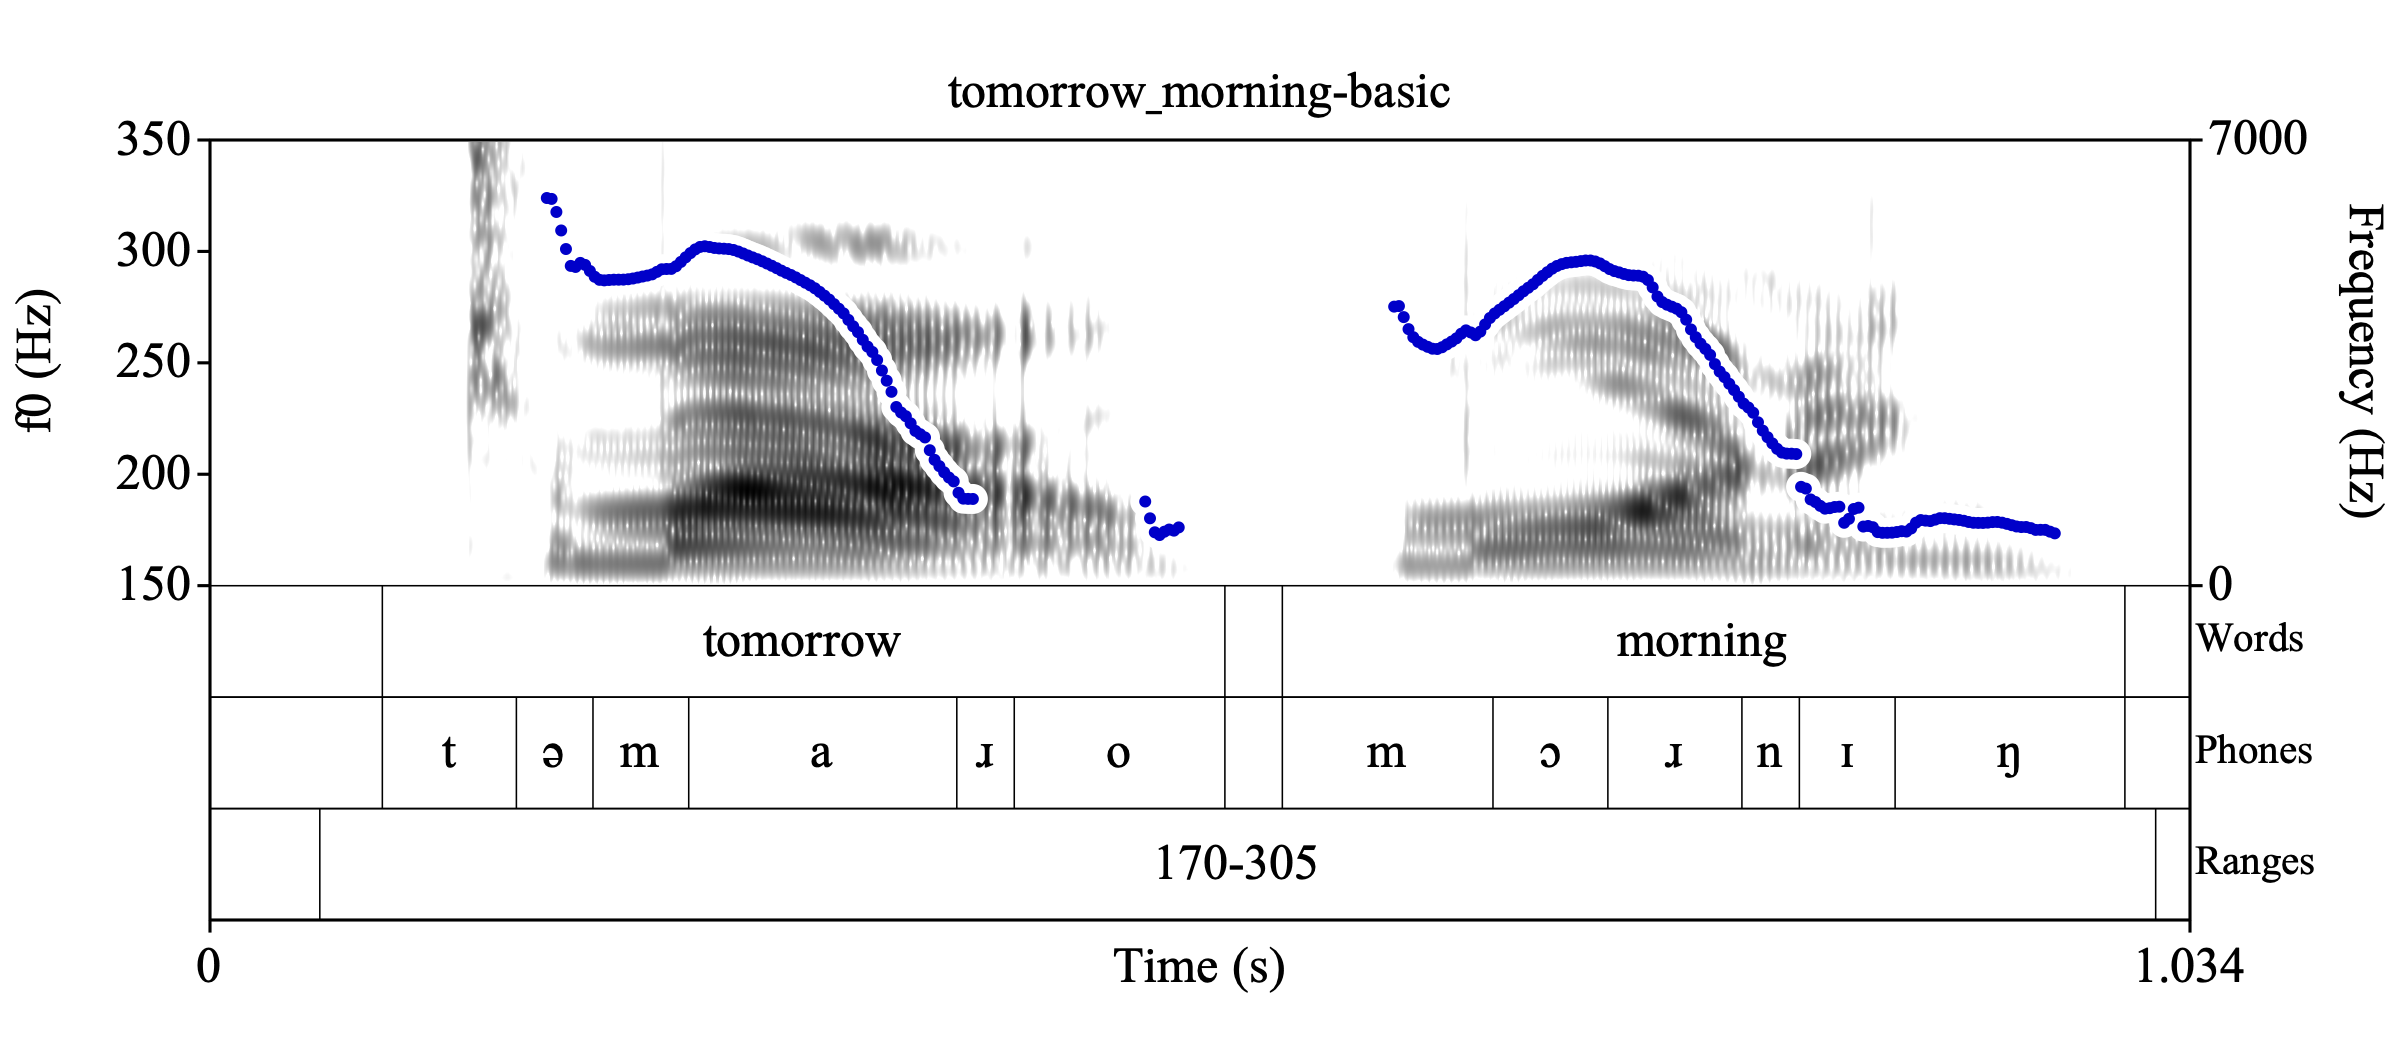
\includegraphics[width=.875\linewidth]{Ranges-tomorrow_morning-basic.png}
%
\caption{This example shows two short words produced with a silence between them, but sharing a single range.%
\label{fig:tomorrow_morning Ranges basic}%
\index{Annotated example, Ranges tier (basic)!tomorrow\_morning}%
}
\end{figure}

\subsection{Levels Tier}\label{sec:levels}

The Levels Tier (also called the \uline{Scaled \textbf{L}evels tier)} is a point tier that reflects the relative scaling of points in the Points tier within each successive range designated in the Ranges tier. The labels on this tier can be automatically added, using a script included with the Praat PoLaR plugin, once the Points tier and the Ranges tier have both been annotated. (Further instructions on using the plugin can be found in chapter \ref{ch:practical}.)

PoLaR uses 5 numbered levels, 1 to 5, where 1 is the lowest f0 band within the current range and 5 is the highest.\footnote{Some informal empirical support for this decision to employ 5 levels within the local range comes from Cole (p.c.), who found that four levels were not sufficient for synthesizing the basic contours of the MAE\_ToBI system, but five levels seemed to suffice.} A basic algorithm (one used by the PoLaR plugin script) divides the Hertz space of the current Range by 5. For example, for a hypothetical range of 100 to 150 Hz, the 50 Hz of the range would be divided into levels of 10 Hz:

\begin{itemize}
\item Level 1: ≥100, ≤ 110
\item Level 2: >110, ≤ 120
\item Level 3: >120, ≤ 130
\item Level 4: >130, ≤ 140
\item Level 5: >140, ≤ 150 \end{itemize}

The Levels value for a given point in the Points tier will be determined by that point’s f0 value in Hz (or the comma-override value), and where it falls in the current 5-part range. So, for this hypothetical range, a point between 140 and 150 Hz (e.g., 143.1) would be level 5, and a point between 110 and 120 (e.g., 119.7) would be a level 2.

Conceptually, the Levels tier divides the pitch space within given range (taken from the Range tier) into 5 equal bands or sub-ranges, as schematized in Figure \ref{fig:tomorrow_morning Levels basic}. In this example, the first point (falling during the [m] of “\langtext{tomorrow}”) corresponds to a turning point whose f0 in the pitch track is located in the top band (shown in red). Accordingly, this point gets assigned a 5 in the levels tier. Likewise the second point, which while slightly higher in f0, is still within the red band representing level 5. The following point, later in the [a] of “\langtext{tomorrow}”, corresponds to a slightly lower f0 that falls within the 4 band (shown in yellow), and therefore gets assigned a level 4. Points marked at both the end of “\langtext{tomorrow}” and the end of “\langtext{morning}” correspond to f0 points in the lowest band (in purple), and are assigned level 1. (Note that in this particular example, there is a point where the pitch tracker is unreliable during “\langtext{tomorrow}”, as the speaker’s voice has become creaky. Recall section \ref{sec:optional-f0-override-labels-for-annotating-pitch-points-without-a-reliable-f0-track}).

\begin{figure}[H]
\centering
%
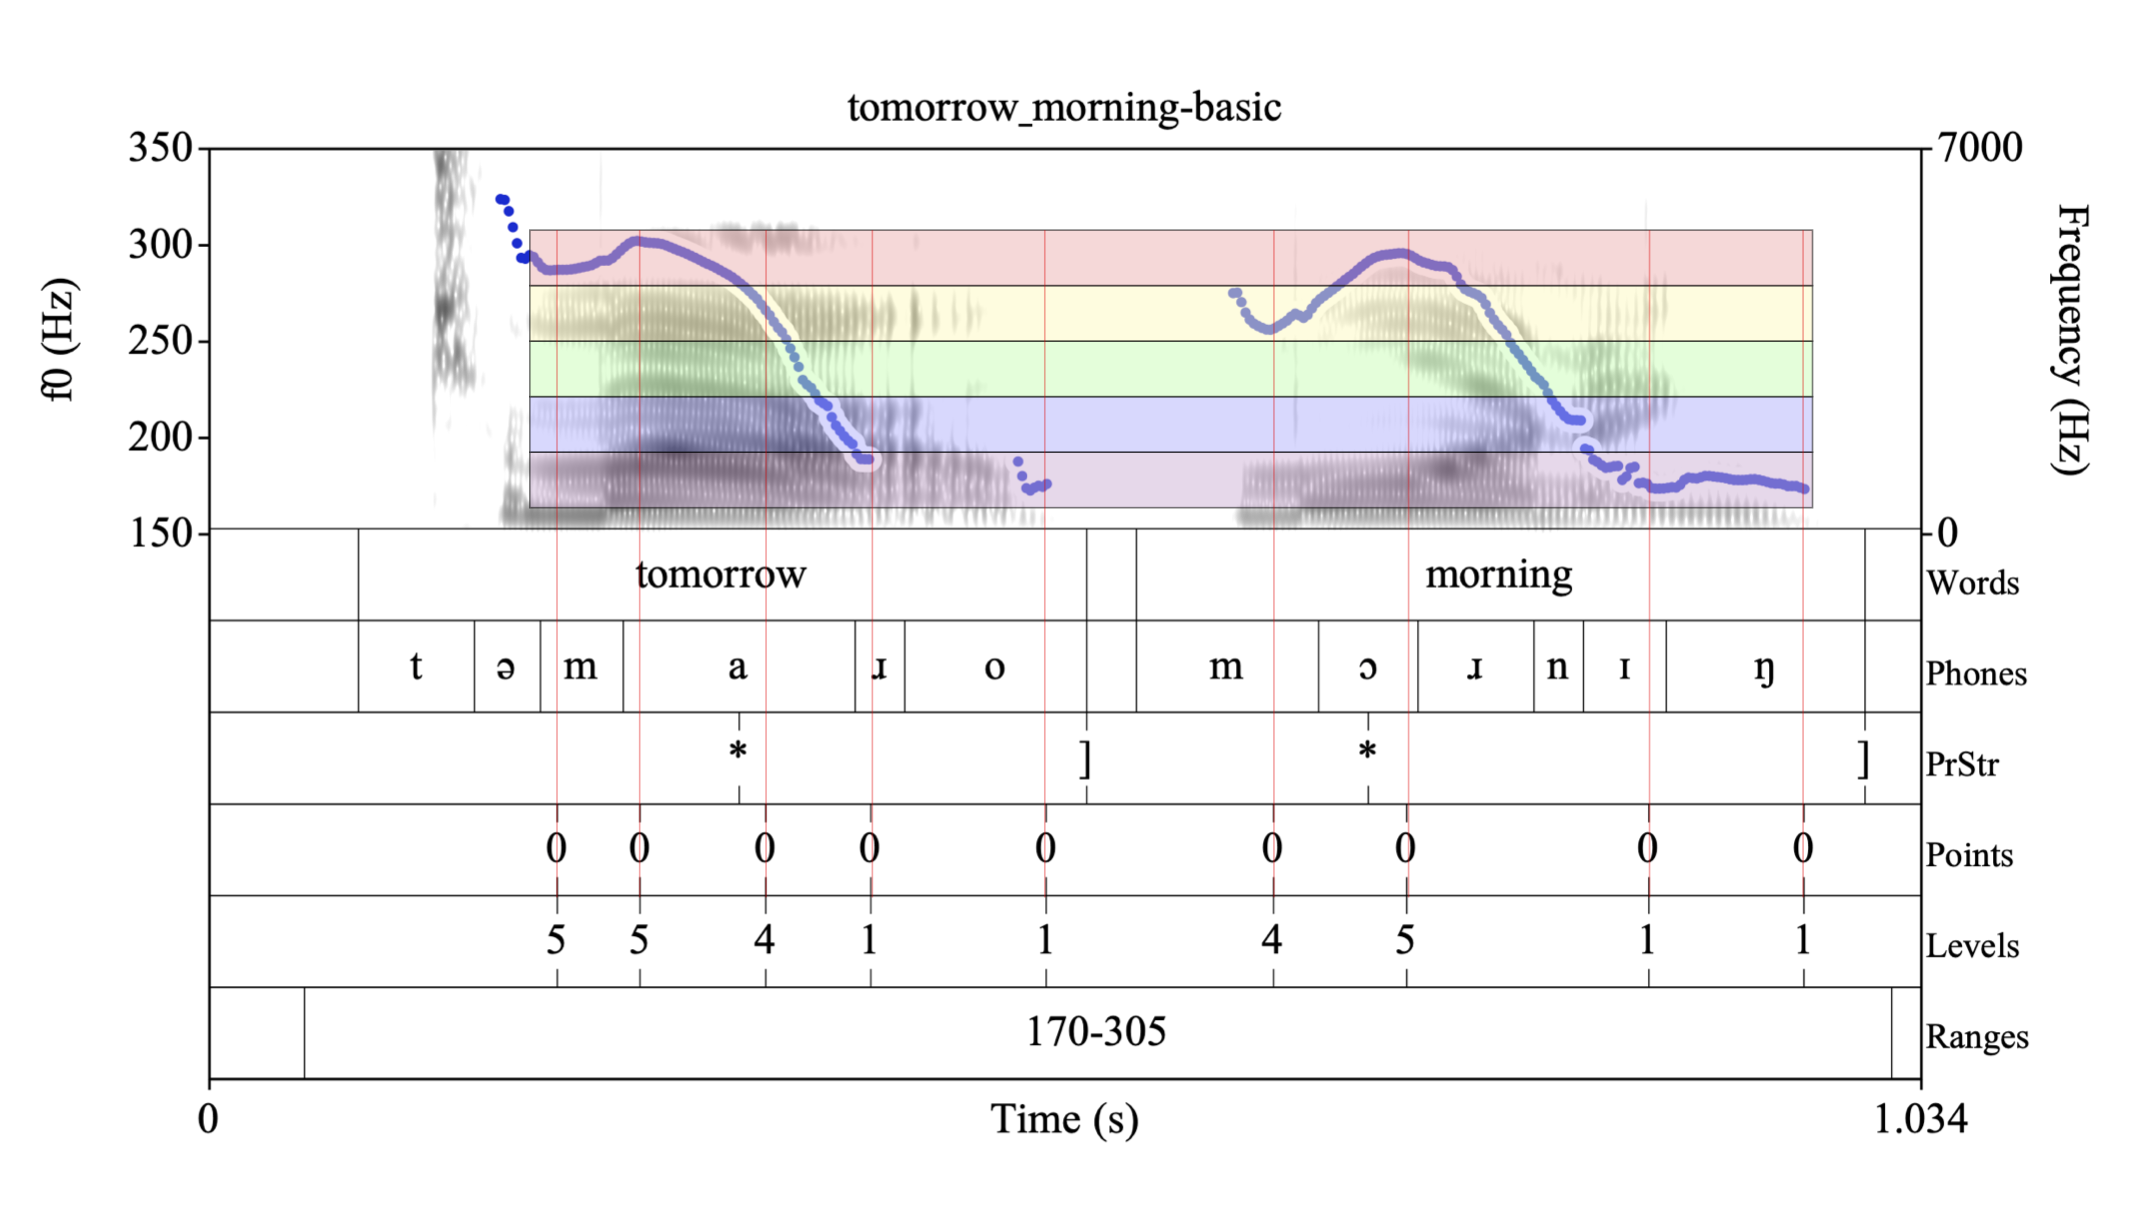
\includegraphics[width=.875\linewidth]{Levels-tomorrow_morning-basic.png}
%
\caption{A visual representation of the five pitch spaces corresponding to Levels annotation.%
\label{fig:tomorrow_morning Levels basic}%
\index{Annotated example, Levels tier (basic)!tomorrow\_morning}%
}
\end{figure}

The main advantage of the Levels tier is that it helps to encode (from the labels in the Ranges tier) what is perceived as categorically high vs. low. That is, the Levels tier captures the labeller’s intuition that a particular f0 event is produced high or low in the speaker’s current selected f0 range, as labelled in the Ranges tier (see section \ref{sec:ranges} above). This reflects the fact that raw f0 values do not adequately specify whether an f0 event realizes a high or a low tonal target, because speakers select different ranges (from within the overall range of possible f0 values that they can produce) for successive portions of an utterance. As noted above, PoLaR provides 5 levels on this tier, which can be automatically determined once the Ranges and Points tiers have been labelled.

For example, the file \texttt{no\_cigar}, shown in Figure \ref{fig:no_cigar Levels basic}, has 2 ranges annotated: 1) from 125-175 Hz for the word “\langtext{close}”, and 2) from 110-145 Hz for the word sequence “\langtext{but no cigar}”. Note that the pitch-accent-related point in the “\langtext{-gar}” of “\langtext{cigar}” is at around 140 Hz, so corresponds to a High in the range for “\langtext{but no cigar}” (as reflected in the level 5 designation, visually represented as the highest colored band in the right side of the figure), but it is only a bit higher (in absolute f0) than the point in “\langtext{close}” that is at 130 Hz, so corresponds to a Low (as reflected by the level 1 designation, visually represented by the lowest colored band in the left side of the figure) in the range for that word.

\begin{figure}[H]
\centering
%
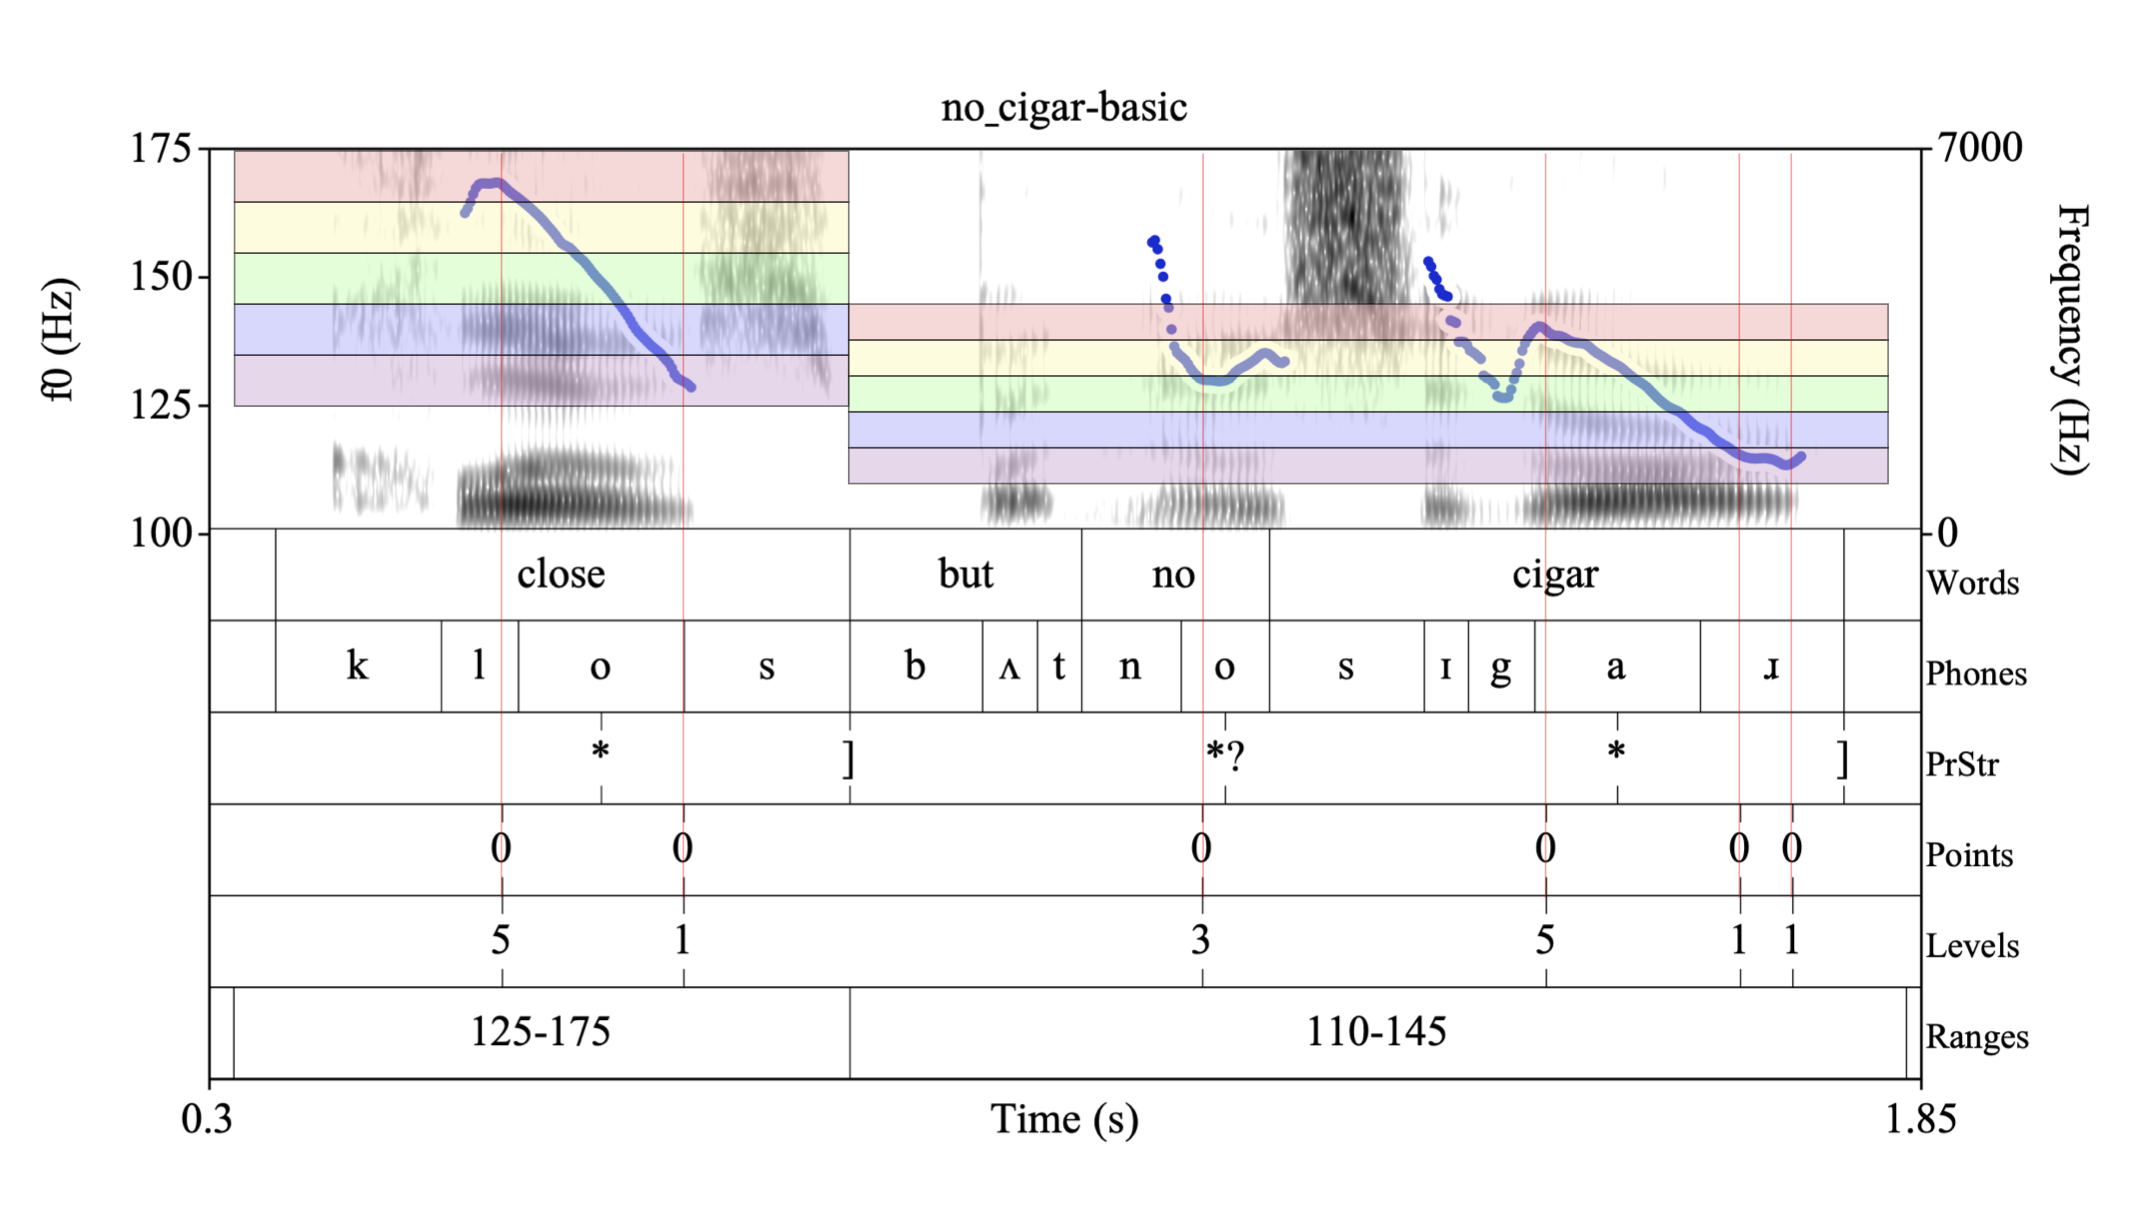
\includegraphics[width=.875\linewidth]{Levels-no_cigar-basic-rainbow.png}
%
\caption[\texttt{no\_cigar}, with Basic labels and overlaid colored bands.]{\texttt{no\_cigar}, with Basic labels on the Points, Levels, and Ranges tiers. The two sets of colored bands correspond to the scaled “level” values, with each set corresponding to one of the Range intervals.%
\label{fig:no_cigar Levels basic}%
\index{Annotated example, Levels tier (basic)!no\_cigar}%
}
\end{figure}


Given how Levels tier labels essentially normalize f0 values, these labels can be used for creating abstractions of the pitch contour, which can be compared directly, across items. To be specific, this production in Figure \ref{fig:no_cigar Levels basic} has 5-1-3-5-1-1 contour, while maybe a different production might have a 5-1-3-5-1-4 contour. What this Levels tier sequence allows for is an easy way to identify that the essential difference is in final pitch movement. In this way, Levels labels can serve as proxies for concepts like “high pitch” or “low pitch”, and may even be usable (in tandem with PrStr labels) to reconstruct phonological labels (e.g., ToBI \textlabel{H*} or \textlabel{H\%}.)

\section{Intonational Contours and Software-Based F0 Tracks}\label{sec:intonational-contours-and-software-based-pitch-tracks}

At this point, we have established how to annotate using PoLaR’s Basic labels, for each tier. Before moving on to the Advanced labelling system, this section takes us on an important digression to discuss the relationship between the intonational contours we aim to recover on the basis of PoLaR labels and the f0 tracks produced by software like Praat, since the f0 tracks are an important cue for labellers of the Points tier.

To review section \ref{sec:terminology}, the intonational contour is an abstract theoretical construct, and the software-based estimated f0 contour is a visualization, produced on the basis of particular settings and an algorithm. In other words, intonational contours and f0 contours are conceptually different. Intonational contours correspond to symbolic objects in the mind of a listener (thus not directly observable) that represent how pitch (a psycho-perceptual phenomenon) changes over time. On the other hand, f0 contours are visualizations corresponding to physical speech signals in which acoustic properties are measured in a programmatic way (which may make errors or produce contours that differ from the intonational contour).

A common goal for an annotator is to keep track of how pitch changes over time —by annotating key elements of the intonational contour— using both auditory perception as well as the f0 contour visualizations (a.k.a. “f0 tracks”). While the f0 track produced by software like Praat\footnote{Note that Praat uses the phrasing “pitch contour” to refer to what we call the “f0 track” or “f0 contour”.} often accurately reflects changes in the intonational contour (hence its usefulness to annotators), f0 tracks are also often discontinuous, jerky, and error-prone in a way that can mislead an annotator if they are not careful. This is because f0 tracks are produced by a mechanistic algorithm that has various adjustable settings (discussed below; see also \href{https://www.fon.hum.uva.nl/praat/manual/Intro_4_2__Configuring_the_pitch_contour.html}{§4.2 of the introductory tutorial to Praat}), and these settings often need to be adjusted. (For more information about how software like Praat produces f0 tracks, see §5 of \citealt{weenink20}.)

In what follows, we will discuss f0 tracks and intonational contours further, including how intonational contours can be approximated, and how f0 tracks are commonly disrupted and how to see “past” disruptions. We will also provide specific guidance and methods for dealing with f0 tracks when doing intonational labelling (in particular, when labelling the Points tier).


\subsection{Intonational Contours and Straight Line Approximations}\label{sec:intonational-contours-and-straight-line-approximations}

As just discussed, the f0 track (i.e., the software-produced estimate of f0 movements, which is produced by an algorithm on the basis of the acoustic signal) consists of a very large number of pitch values (by default, Praat estimates 100 f0 values per second). The idea behind the Points tiers labels is that, at an abstract level, a pitch contour can be defined by a relatively much smaller number of observations (perhaps just a handful for a short utterance). Following in the footsteps of the IPO tradition (e.g., \citealt{t-hartcollier75} and \citealt{t-hart-90}), we have described this in terms of “straight line approximations” (as discussed in section \ref{sec:identifying-necessary-points-labels-with-straight-line-approximations}). In this section we will discuss more on the relationship of Points tier labels and straight line approximations.

A major insight of the IPO framework is that straight line approximations based on a very small number of f0 turning points can be perceptively the same as original recording. (The IPO approximation process is described in works like \citealt{dutoit97} and \citealt{rao12}.) When annotators create a straight line approximation, they are essentially reducing an f0 track to the core pitch turning points. This regularly requires the annotator to ignore movements in the f0 track that are not mirrored in auditory perception (such as those due to microprosody or software errors, as described in sections \ref{sec:software-effects}–\ref{sec:voice-quality-effects}). It also involves ignoring some of the more gradual f0 turning points that define scoop- or dome-shaped contours (instead reducing them to maybe one or two points). (That is, some sudden f0 changes can be ignored, and some gradual changes can be reduced to single pitch turning points.) Repeating some of what is in section \ref{sec:identifying-necessary-points-labels-with-straight-line-approximations}, we provide some guidance on how to identify how many Points labels are necessary. The first piece of guidance we provide here is that we suggest adding Points labels one at a time –erring on the side of over-labelling– to faithfully reproduce the major movements in the f0 track. The second is, to cull the labels that are unnecessary for producing a faithful straight line approximation. When in doubt whether a Point is necessary or superfluous, labellers ought to compare straight line approximations where one includes the Point and the other does not. (If they sound perceptually the same, the Point can be removed.) 

Consider the examples in Fig. \ref{fig:enemy original and resynth} below. The original (more true-to-form) pitch track (on the left) depends on identifying pitch points at a regular (and very high) interval, while the straight-line approximation depends on just the six points identified in the PoLaR Points tier. Even to a trained ear, the resynthesized utterance in the figure on the right is perceptibly the same. In this way, PoLaR can be seen as enabling researchers to remove all but the pitch points “that matter”. PoLaR provides a means (the Points tier labels) to identify the coordinates (for axes of time and pitch space) that can define the intonational contour, and the PoLaR plugin for Praat can be used to resynthesize straight line approximations on the basis of those Points labels. (See section \ref{sec:identifying-necessary-points-labels-with-straight-line-approximations} for more details about this.)

\begin{figure}[H]
\centering
%
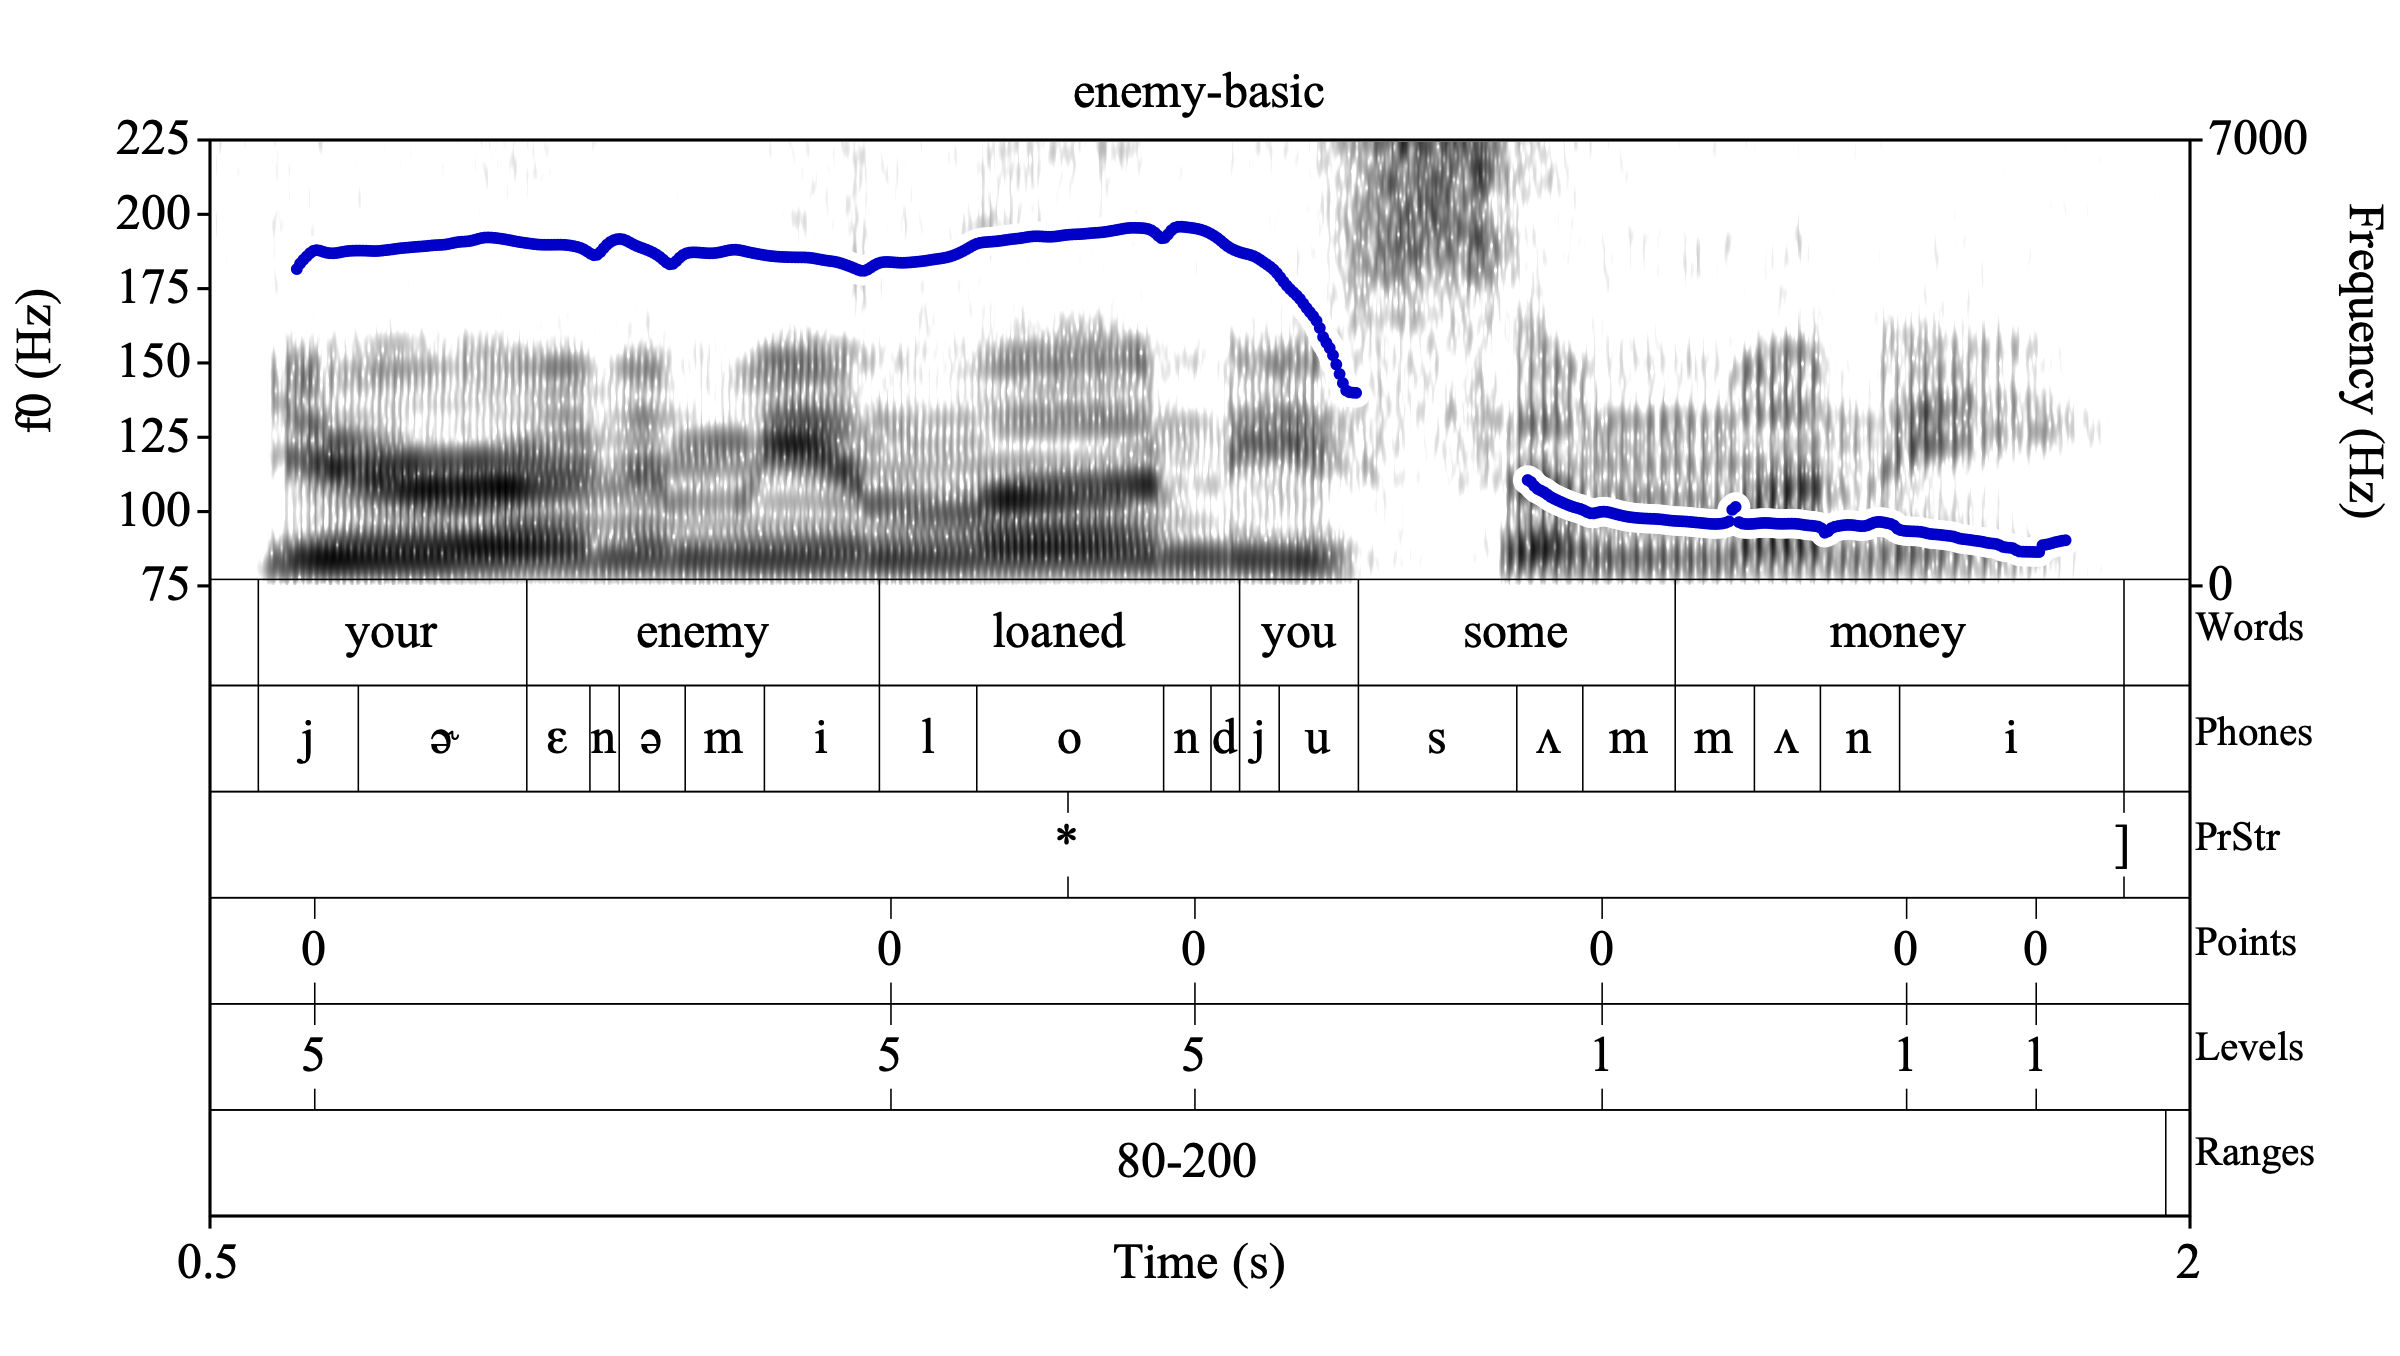
\includegraphics[width=.485\linewidth]{Contours-enemy.png}~~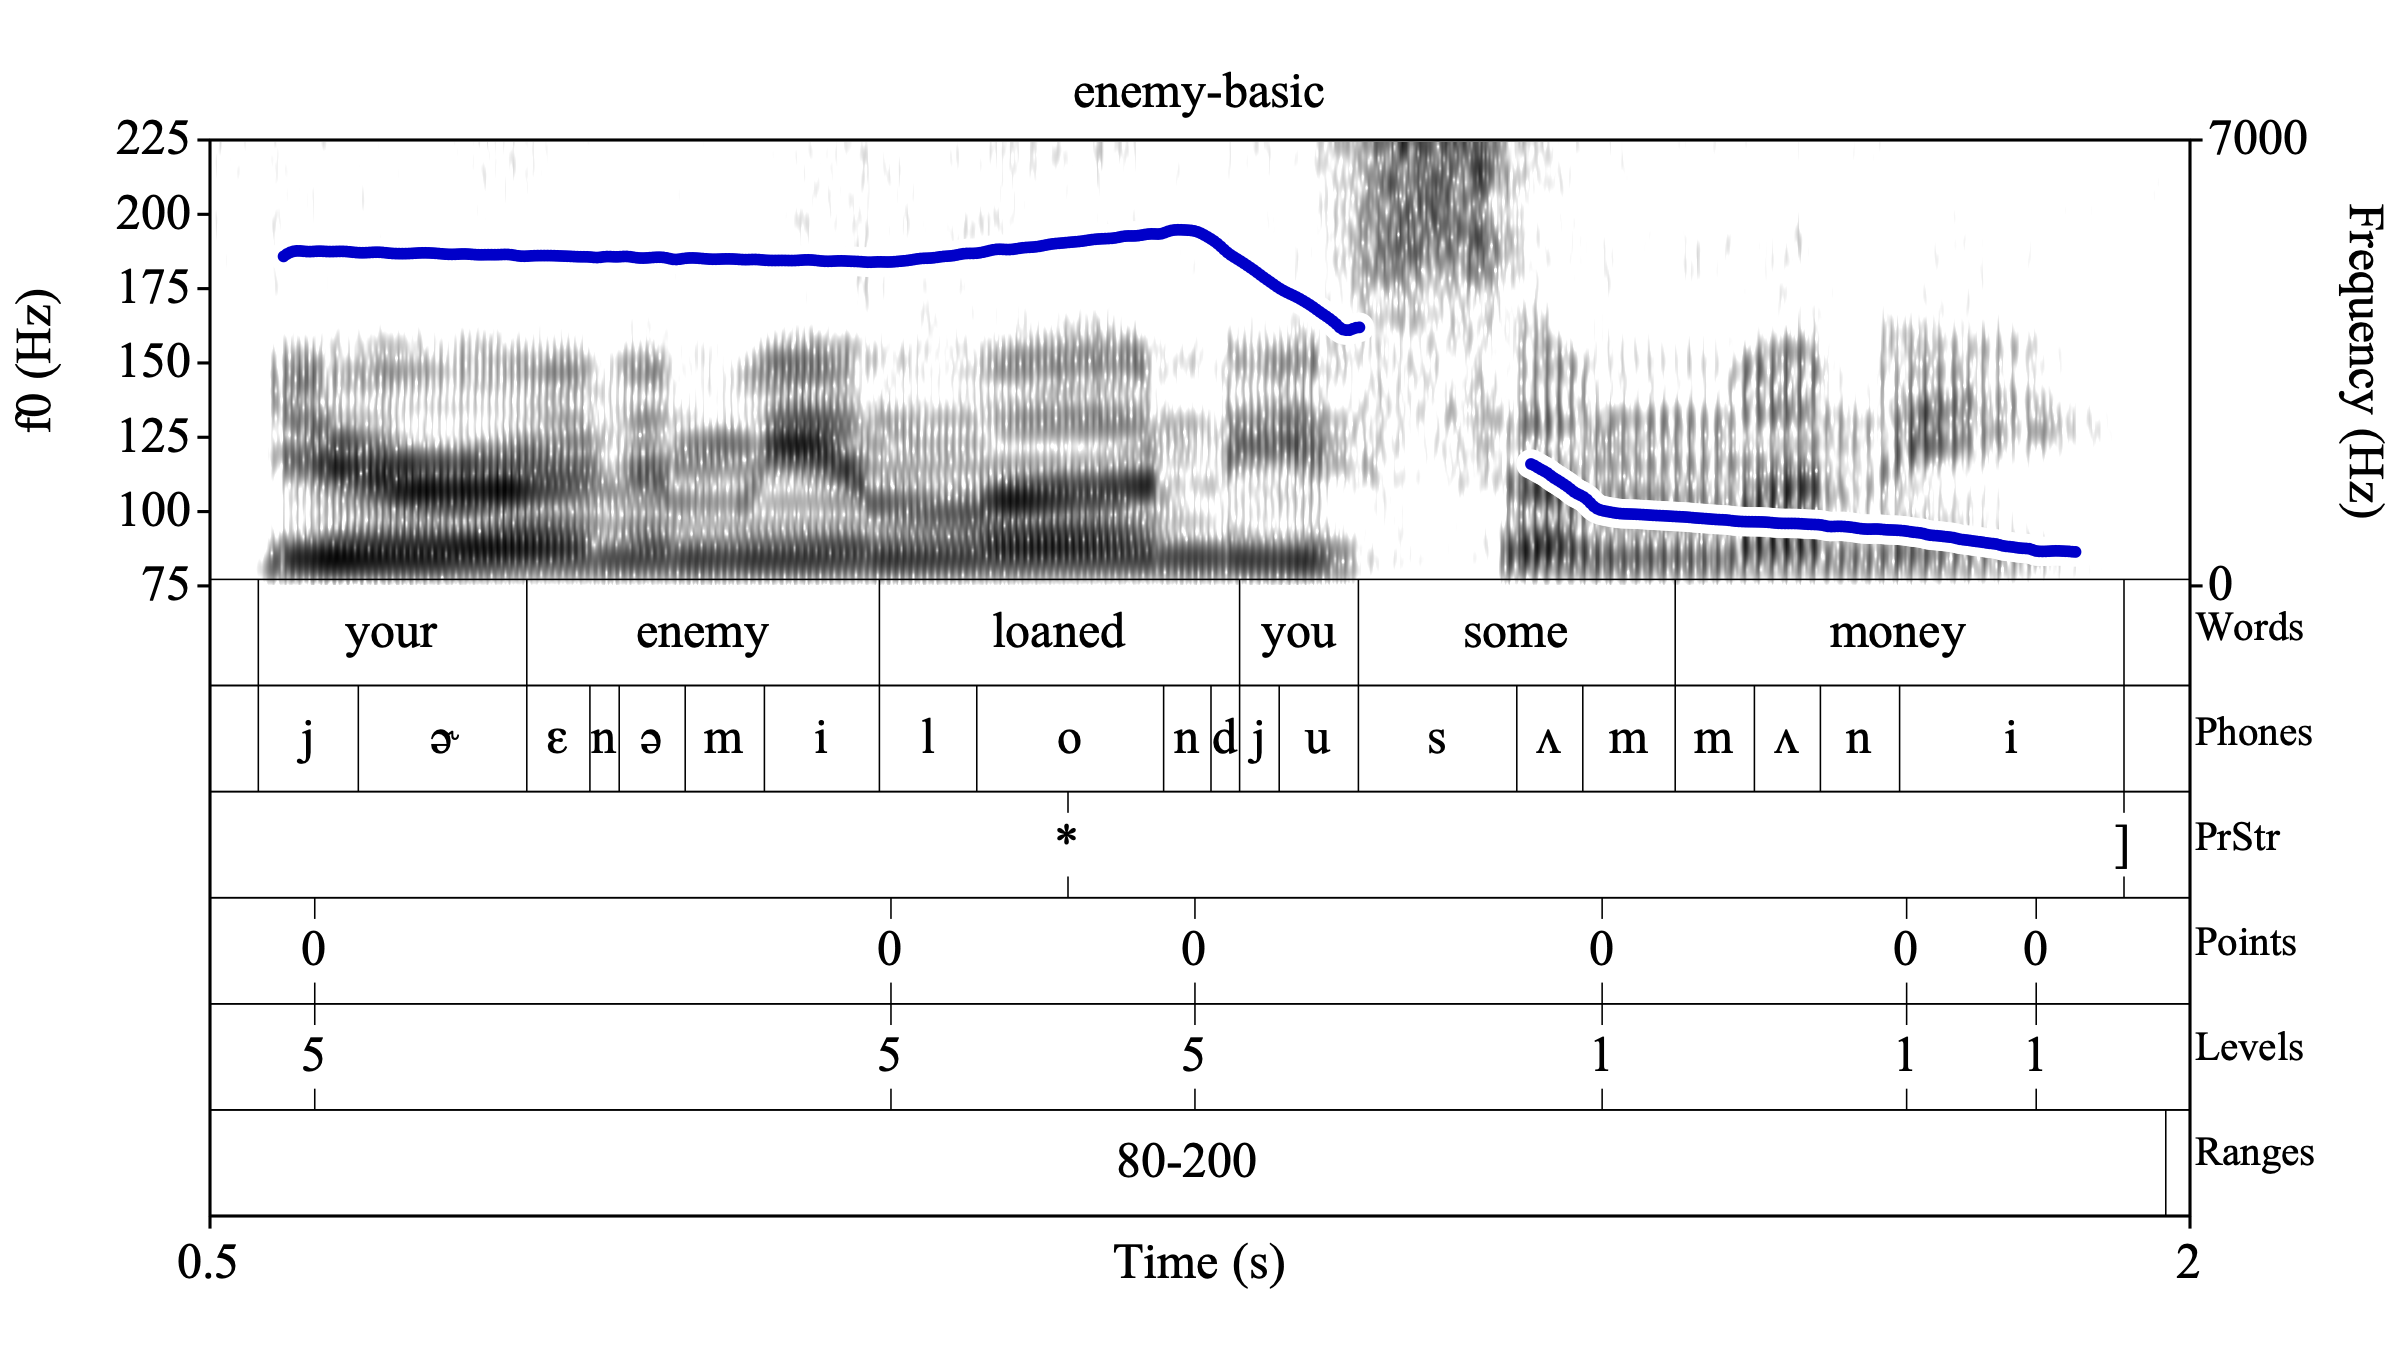
\includegraphics[width=.485\linewidth]{Contours-enemy-resynth.png}
%
\caption{A recording with PoLaR labels and its resynthesized straight line approximation, created with a script from the PoLaR plugin in Praat.%
\label{fig:enemy original and resynth}%
}
\end{figure}

Even with such an impoverished version of the pitch track (such as \texttt{enemy-resynth}), and even to a trained ear, the “real” and “resynthesized” examples can be indistinguishable. On the other hand, removing some of these remaining turning points may result in a somewhat “unnatural” sound (in the sense that, at least, a trained ear could distinguish the resynthesized version from the original). Given that this straight line approximation sounds both natural and identical to the original, we argue that our Points tier annotation of six pitch points in Fig. \ref{fig:enemy original and resynth} is sufficient to capture the meaningful turning points. This same technique of manipulating pitch into a straight line approximation can be applied to any recording, to see whether the correct number of Points have been labelled.

Practically speaking, we assume that experienced labellers will be able to distinguish significant turning points from noisy variation, but caution is urged in eliminating those that would impact the shape of the contour. Our experience with the Tonal Center of Gravity dictates that individual Turning points are not perceptually salient; it is the set of turning points that creates a perceptually useful shape. 

In this way, using the Points tier labels to construct a straight-line approximation of the f0 track (which itself is based on the acoustic signal) can be used to help identify the shape of the (abstract phonological) intonational contour.\footnote{Note: this series of acoustic cues in the signal does not, for various reasons (including the phonetics-phonology interface, technical abilities of the pitch tracking software, microprosody, etc.), perfectly reflect the intonational contour, which is an abstract representation (defined in terms of phonological categories and structures).} As such, these straight line approximations have the potential for understanding more about the phonological representation of intonational contours.

\subsection{Sources of f0 track disruptions}\label{sec:a-brief-overview-of-sources-of-pitch-track-disruptions}

As mentioned, while the f0 track is often reflective of the perceptual changes in pitch, there are also regular ways in which the f0 track can differ from the intonational contour. For example, an annotator may perceive the pitch of a portion of the utterance as being steady or moving fluidly, while the f0 track of that region shows a discontinuous f0 contour or one that suddenly jumps up\slash down. Thus, if the labeller over-trusts the visualization in the f0 track (overriding how their auditory pitch perception), this may cause a labeller to label extraneous Points labels to capture movements that are not actually part of the speaker’s intonational contour. (Conversely, the visualization may not seem to show f0 movements even where a labeller auditorily perceives one.) In this section, we discuss some of the more common specific f0 tracking problems that occur, the contexts in which they are likely to arise, and the conventions that have arisen over the years among prosodic labellers for dealing with them.

One class of problems occurs when the software-based f0 estimator is disrupted, leading to breaks in the f0 track. A second kind of problem occurs when contextual factors in the speech\slash recording context distort or influence the f0 track, even though a listener’s perception of the pitch contour is not disrupted by these events. Both of these scenarios can challenge the labeller by complicating the issue of determining where Points labels should(n’t) be added.

When in doubt, the annotator is encouraged to \emph{trust their perception}, because the human mind is especially well-tuned to compensate for these disruptions (producing the abstract and “smoothed” intonation contour, on the basis of intonational competence) while software like Praat is designed to keep track of all f0 movements.

\subsubsection{Software effects}\label{sec:software-effects}

One very common way in which f0 tracks end up as inaccurate (meaning not reflecting listeners’ perception of the pitch) has to do with software settings. Most speech applications (such as Praat) must be calibrated regularly (e.g., re-calibrated for each speaker) to get accurate f0 displays.

An example of settings that can greatly impact f0 tracks is the Pitch range minimum\slash maximum values (in Praat, these are found in Pitch > Pitch settings, in an editor window, when viewing Sound objects). What these settings do is tell the algorithm what the minimum\slash maximum \emph{possible} f0 values are; that is, the algorithm will not entertain the possibility that the f0 values dip below the minimum or above the maximum. As such, if the minimum is set too high (e.g., the minimum is set to 100Hz but the actual f0 gets as low as 75Hz), the software will often produce an f0 track with plotted values that are too high (e.g., plotting f0 values at 160Hz where they ought to be 80Hz; see also §\ref{sec:pitch-halving-and-doubling}). Annotators are encouraged to tailor the Pitch range values for speakers, noting that deeper voiced people typically stay within a range of around 60-300Hz, and higher voiced people typically stay within a range of around 100-500Hz, but this can vary quite a bit from person-to-person (and even from recording to recording).

In addition, Praat (\citealt{praat}) provides various other pitch-related settings, for which we provide values we have found to be helpful in doing intonational analysis of human speech; these are the settings used to produce the figures of f0 tracks in this monograph. (The menus referenced below are found in an editor window).

\begin{itemize}
\item Settings for Time Step analysis (found in \texttt{View> Time step settings}\ldots):
	\begin{itemize}
		\item Time step strategy = fixed
		\item Fixed time step (s) = 0.0025
	\end{itemize} 
\item Advanced Pitch settings (found in \texttt{Pitch> Advanced pitch settings}\ldots):
	\begin{itemize}
		\item Max. number of candidates=15
		\item Very accurate=true
		\item Silence threshold=0.03
		\item Voicing threshold=0.5
		\item Octave cost=0.05
		\item Octave jump cost=0.5
		\item Voiced/Unvoiced cost=0.2
	\end{itemize}
\item[] (\textit{You may find it beneficial to adjust these settings further, in particular recordings, to minimize spurious\slash inaccurate f0 measurements. However, doing so may result in f0 tracks that look different from the ones in this monograph.})
\end{itemize}

Changing these settings may affect the f0 track – for example, changing the voicing threshold and octave jump costs can lead to f0 dropout or spurious f0 readings. This should be taken to reinforce the fact that f0 tracks are meant only as a guide to annotators, and annotators are encouraged to diverge from it when their auditory perception suggests. 

While adjusting software settings (especially Pitch Range minimum\slash maximum) is a way to counteract f0 track disruptions, some f0 disruptions cannot be amended to yield an accurate f0 track, due to insurmountable interference from environmental\slash recording factors (e.g., background noise). In these cases, as described in section \ref{sec:optional-f0-override-labels-for-annotating-pitch-points-without-a-reliable-f0-track}, labellers are encouraged to use their intuition and perception to note an f0 estimate, if appropriate and possible. 

\subsubsection{Pitch halving and doubling}\label{sec:pitch-halving-and-doubling}

Sometimes during a recording, the f0 track will suddenly jump or fall – with the measured f0 jumping from say 199Hz to 97Hz (or vice-versa) from one measured f0 point to the next. When suddenly dropping down by a factor of 2, this is pitch halving. Conversely, when suddenly jumping up by a factor of 2, this is pitch doubling. (The factor of 2 difference is due to how Praat measures f0. Because these jumps are related to the f0 measuring algorithm, they are not always exactly a factor of 2; however, factor-of-2 jumps\slash drops are especially common.) 

In other words, pitch halving and pitch doubling involve a change in measured f0 is immediate and significant – faster than the vocal folds can typically change. An example of pitch halving is given in Figure \ref{fig:to volunteer-halved f0-tracking}, and an example of pitch doubling is given in Figure \ref{fig:rutabaga f0-tracking}.

\begin{figure}[H]
\centering
%
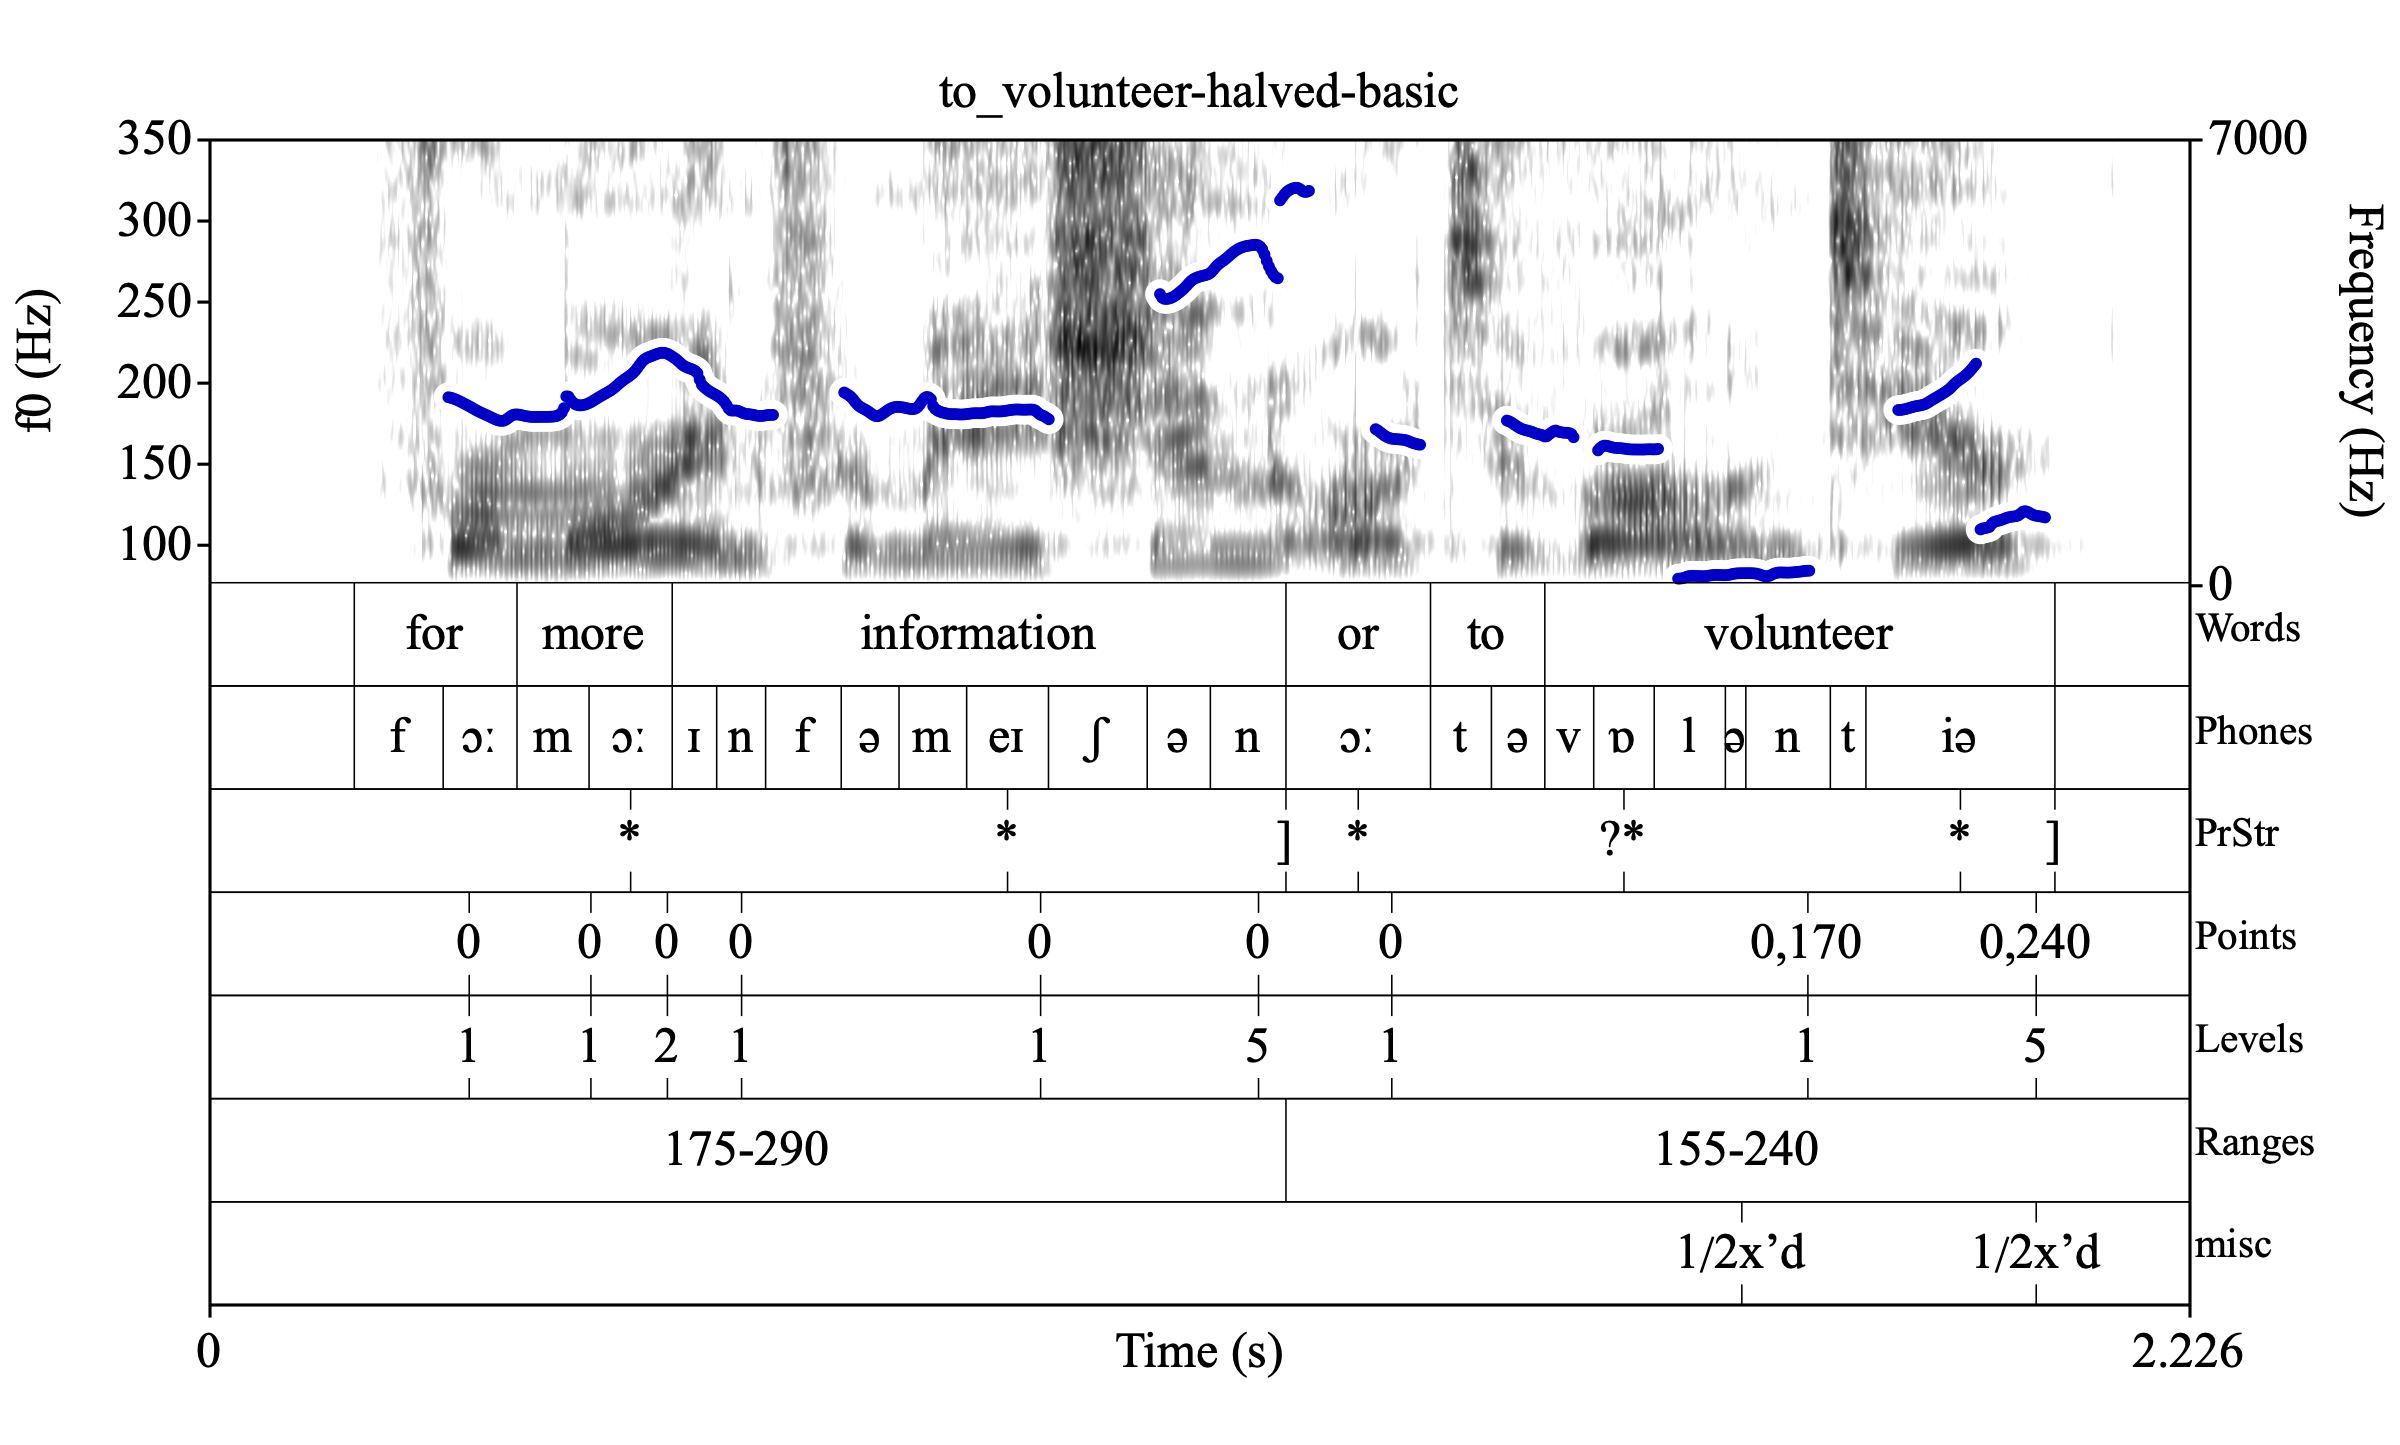
\includegraphics[width=.875\linewidth]{Appendix-to_volunteer-halved.png}
%
\caption{Example of pitch halving.%
\label{fig:to volunteer-halved f0-tracking}%
\index{Annotated example, f0 tracking!to\_volunteer-halved}%
}
\end{figure}

\begin{figure}[H]
\centering
%
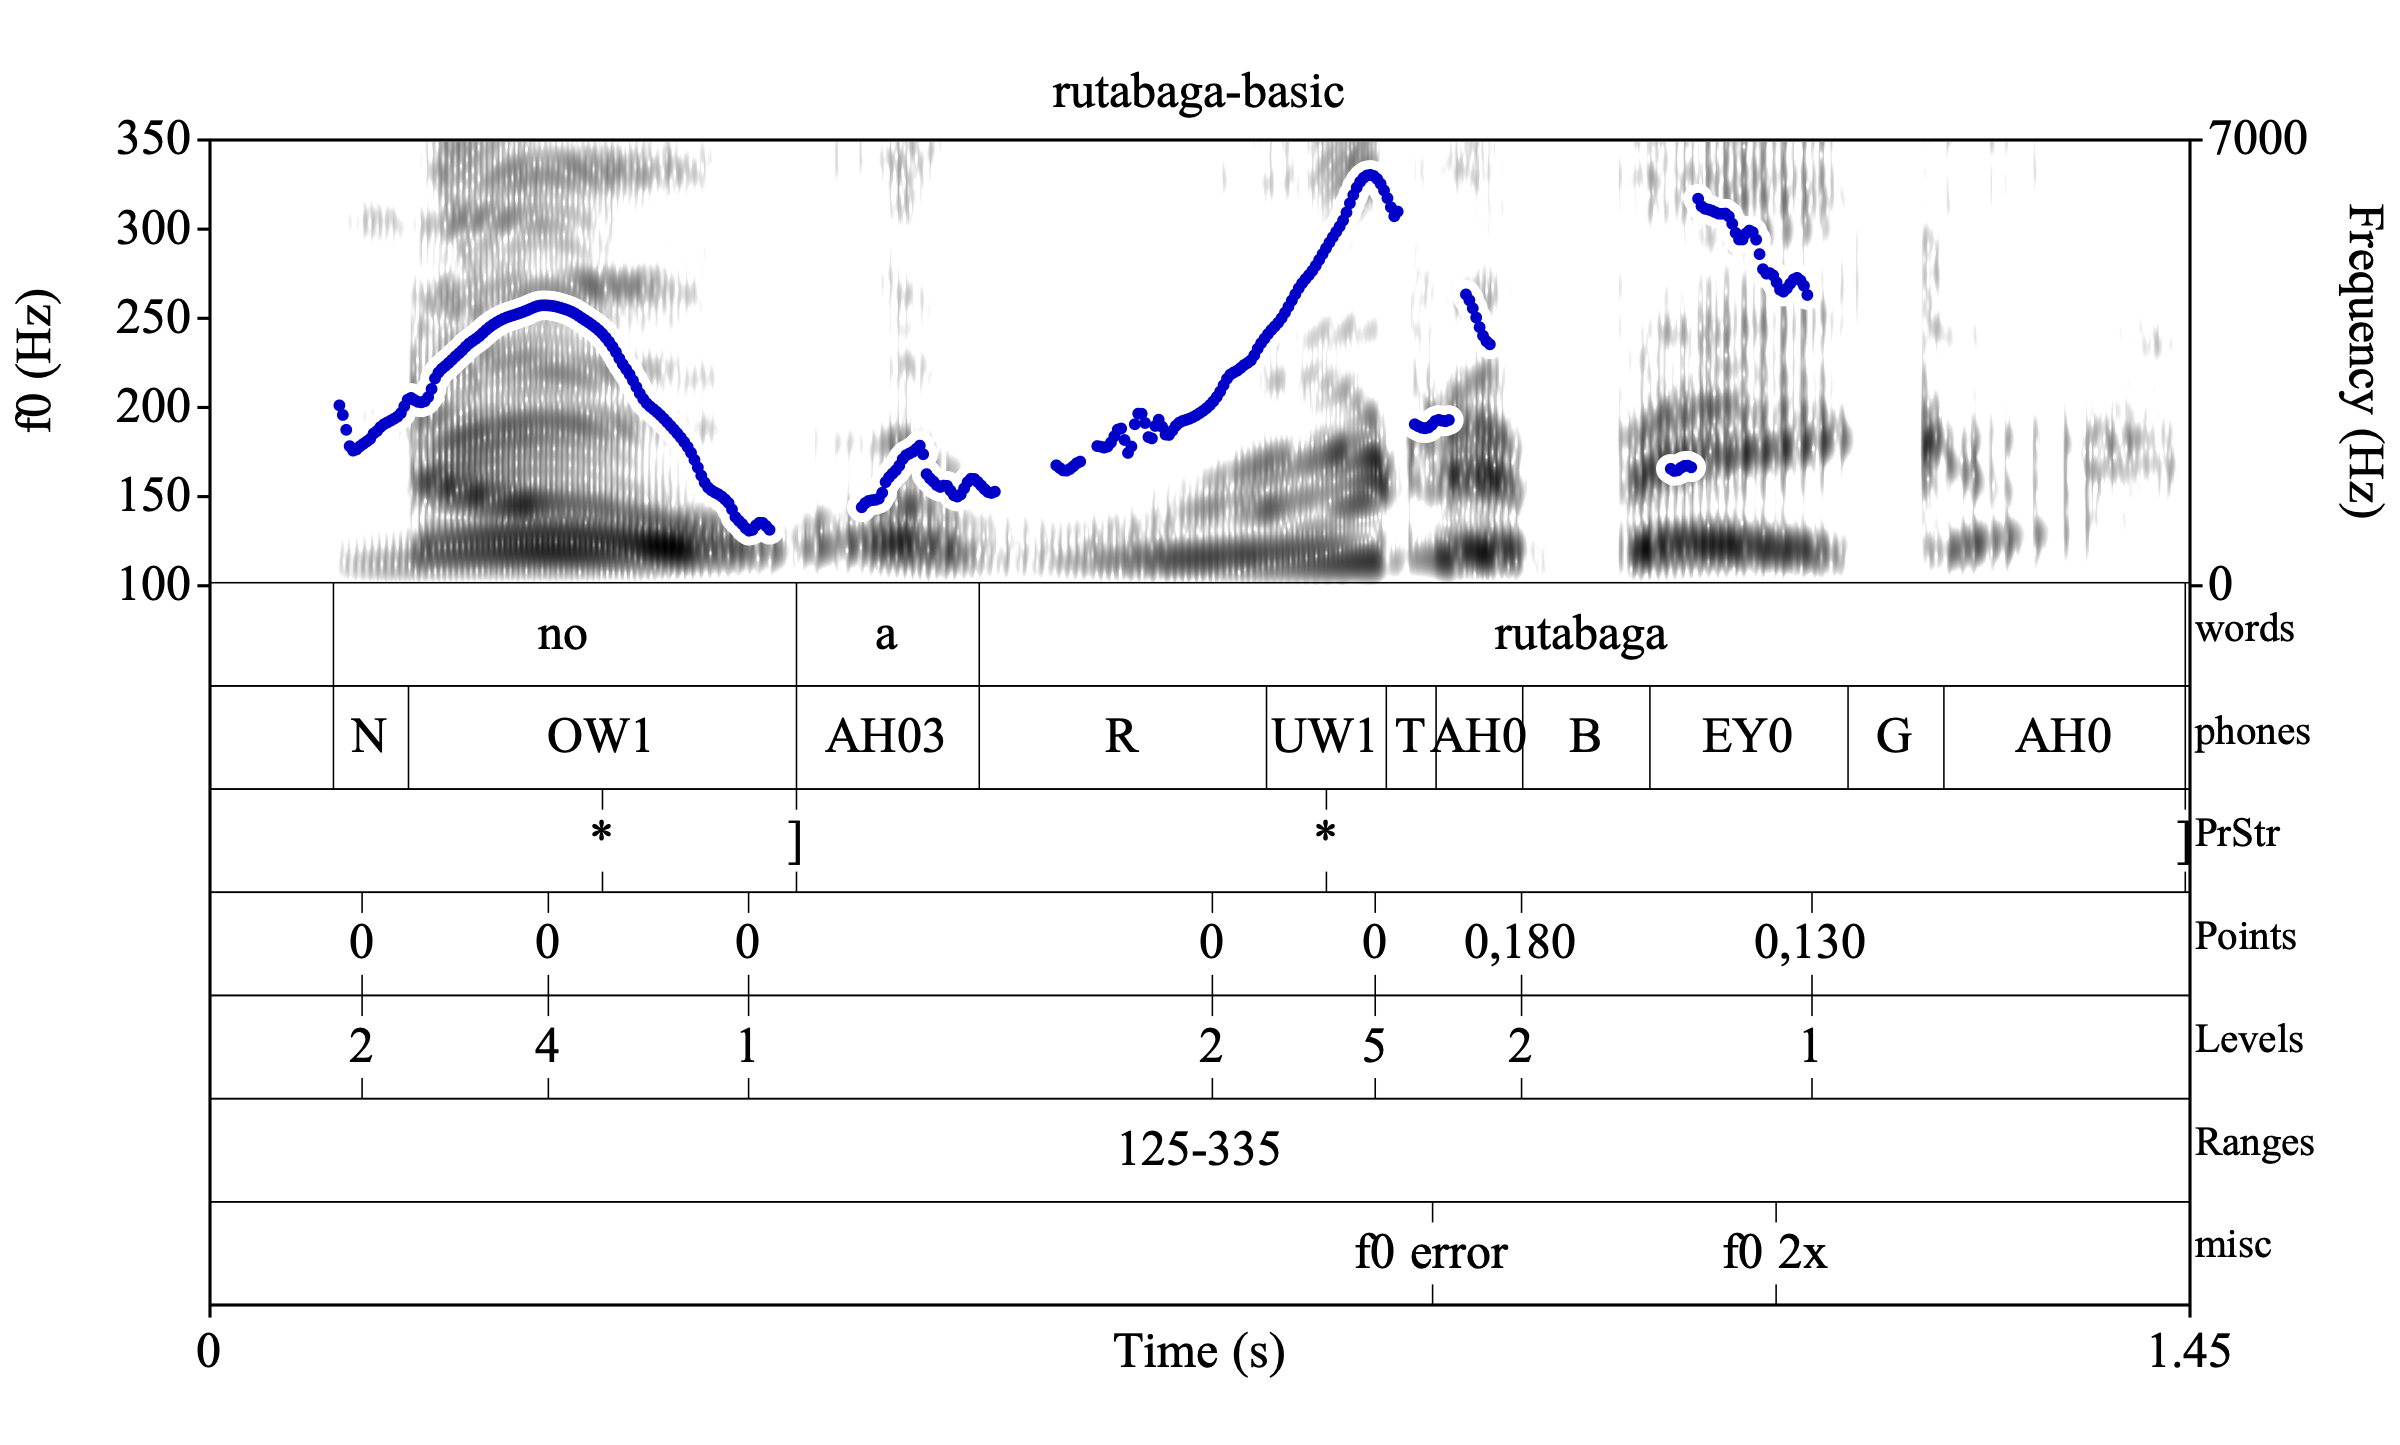
\includegraphics[width=.875\linewidth]{Contours-rutabaga-basic.png}
%
\caption{Example of pitch doubling.%
\label{fig:rutabaga f0-tracking}%
\index{Annotated example, f0 tracking!rutabaga}%
}
\end{figure}

We provide some hints to help identify what is “immediate and significant”, a labeller can rely on.
First and foremost, a labeller should trust their auditory perception. If the labeller perceives that the pitch is locally low, but the f0 track looks locally high, this could be due to pitch doubling; for example, at the end of “\langtext{rutabaga}” in Fig. \ref{fig:to volunteer-halved f0-tracking}, the pitch is perceived to continually fall, but it shows as almost as high as the preceding peak. Similarly, if the f0 shows a low that sounds high to the labeller, this may be halving. In these cases, the f0 tracker commonly measures f0 values that are either half (e.g., the pitch tracker shows 70 Hz, where listeners perceive pitch corresponding to 140 Hz) or double (e.g., the pitch tracker shows 140 Hz, where listeners perceive pitch corresponding to 70 Hz) the “true” pitch for the speech.

A second way is to try changing the pitch range settings. If the pitch range settings are set to 100-200Hz, but the true f0 max is 250Hz, any f0 that is truly between 200Hz and 250Hz will be mis-measured – often as pitch halving, showing as 100-125Hz. This is because, if a speaker reaches a peak f0 over 500Hz but your maximum is set at 400Hz, the f0 tracker will be forced to estimate points within that range. Adjusting the setting for the pitch range maximum to be 250Hz will often resolve this sort of pitch halving. However, there are cases of pitch halving\slash doubling that persist even when the pitch range is set appropriately (such as Fig. \ref{fig:rutabaga f0-tracking}).

The third way we name here to check perception is to make use of the tool for resynthesizing straight line approximations (as described in section \ref{sec:identifying-necessary-points-labels-with-straight-line-approximations}). In Fig. \ref{fig:to volunteer-halved f0-tracking}, there are no Points labels during the pitch-halved regions, and resynthesizing yields a recording that sounds like the original. Had the drop in measured f0 been faithful to a drop in the true f0, such a resynthesis without Points labels encoding the drops would sound like a different contour. For Fig. \ref{fig:rutabaga f0-tracking}, a comma override is used; at the time of the final Points label, the f0 tracker reads about 260Hz, so a comma override of \textlabel{,130} (i.e., half the measured value) is used. The resynthesis of Fig. \ref{fig:rutabaga f0-tracking} is shown in Fig. \ref{fig:rutabaga-resynth f0-tracking}, below, and it sounds very much like the original.

\begin{figure}[H]
\centering
%
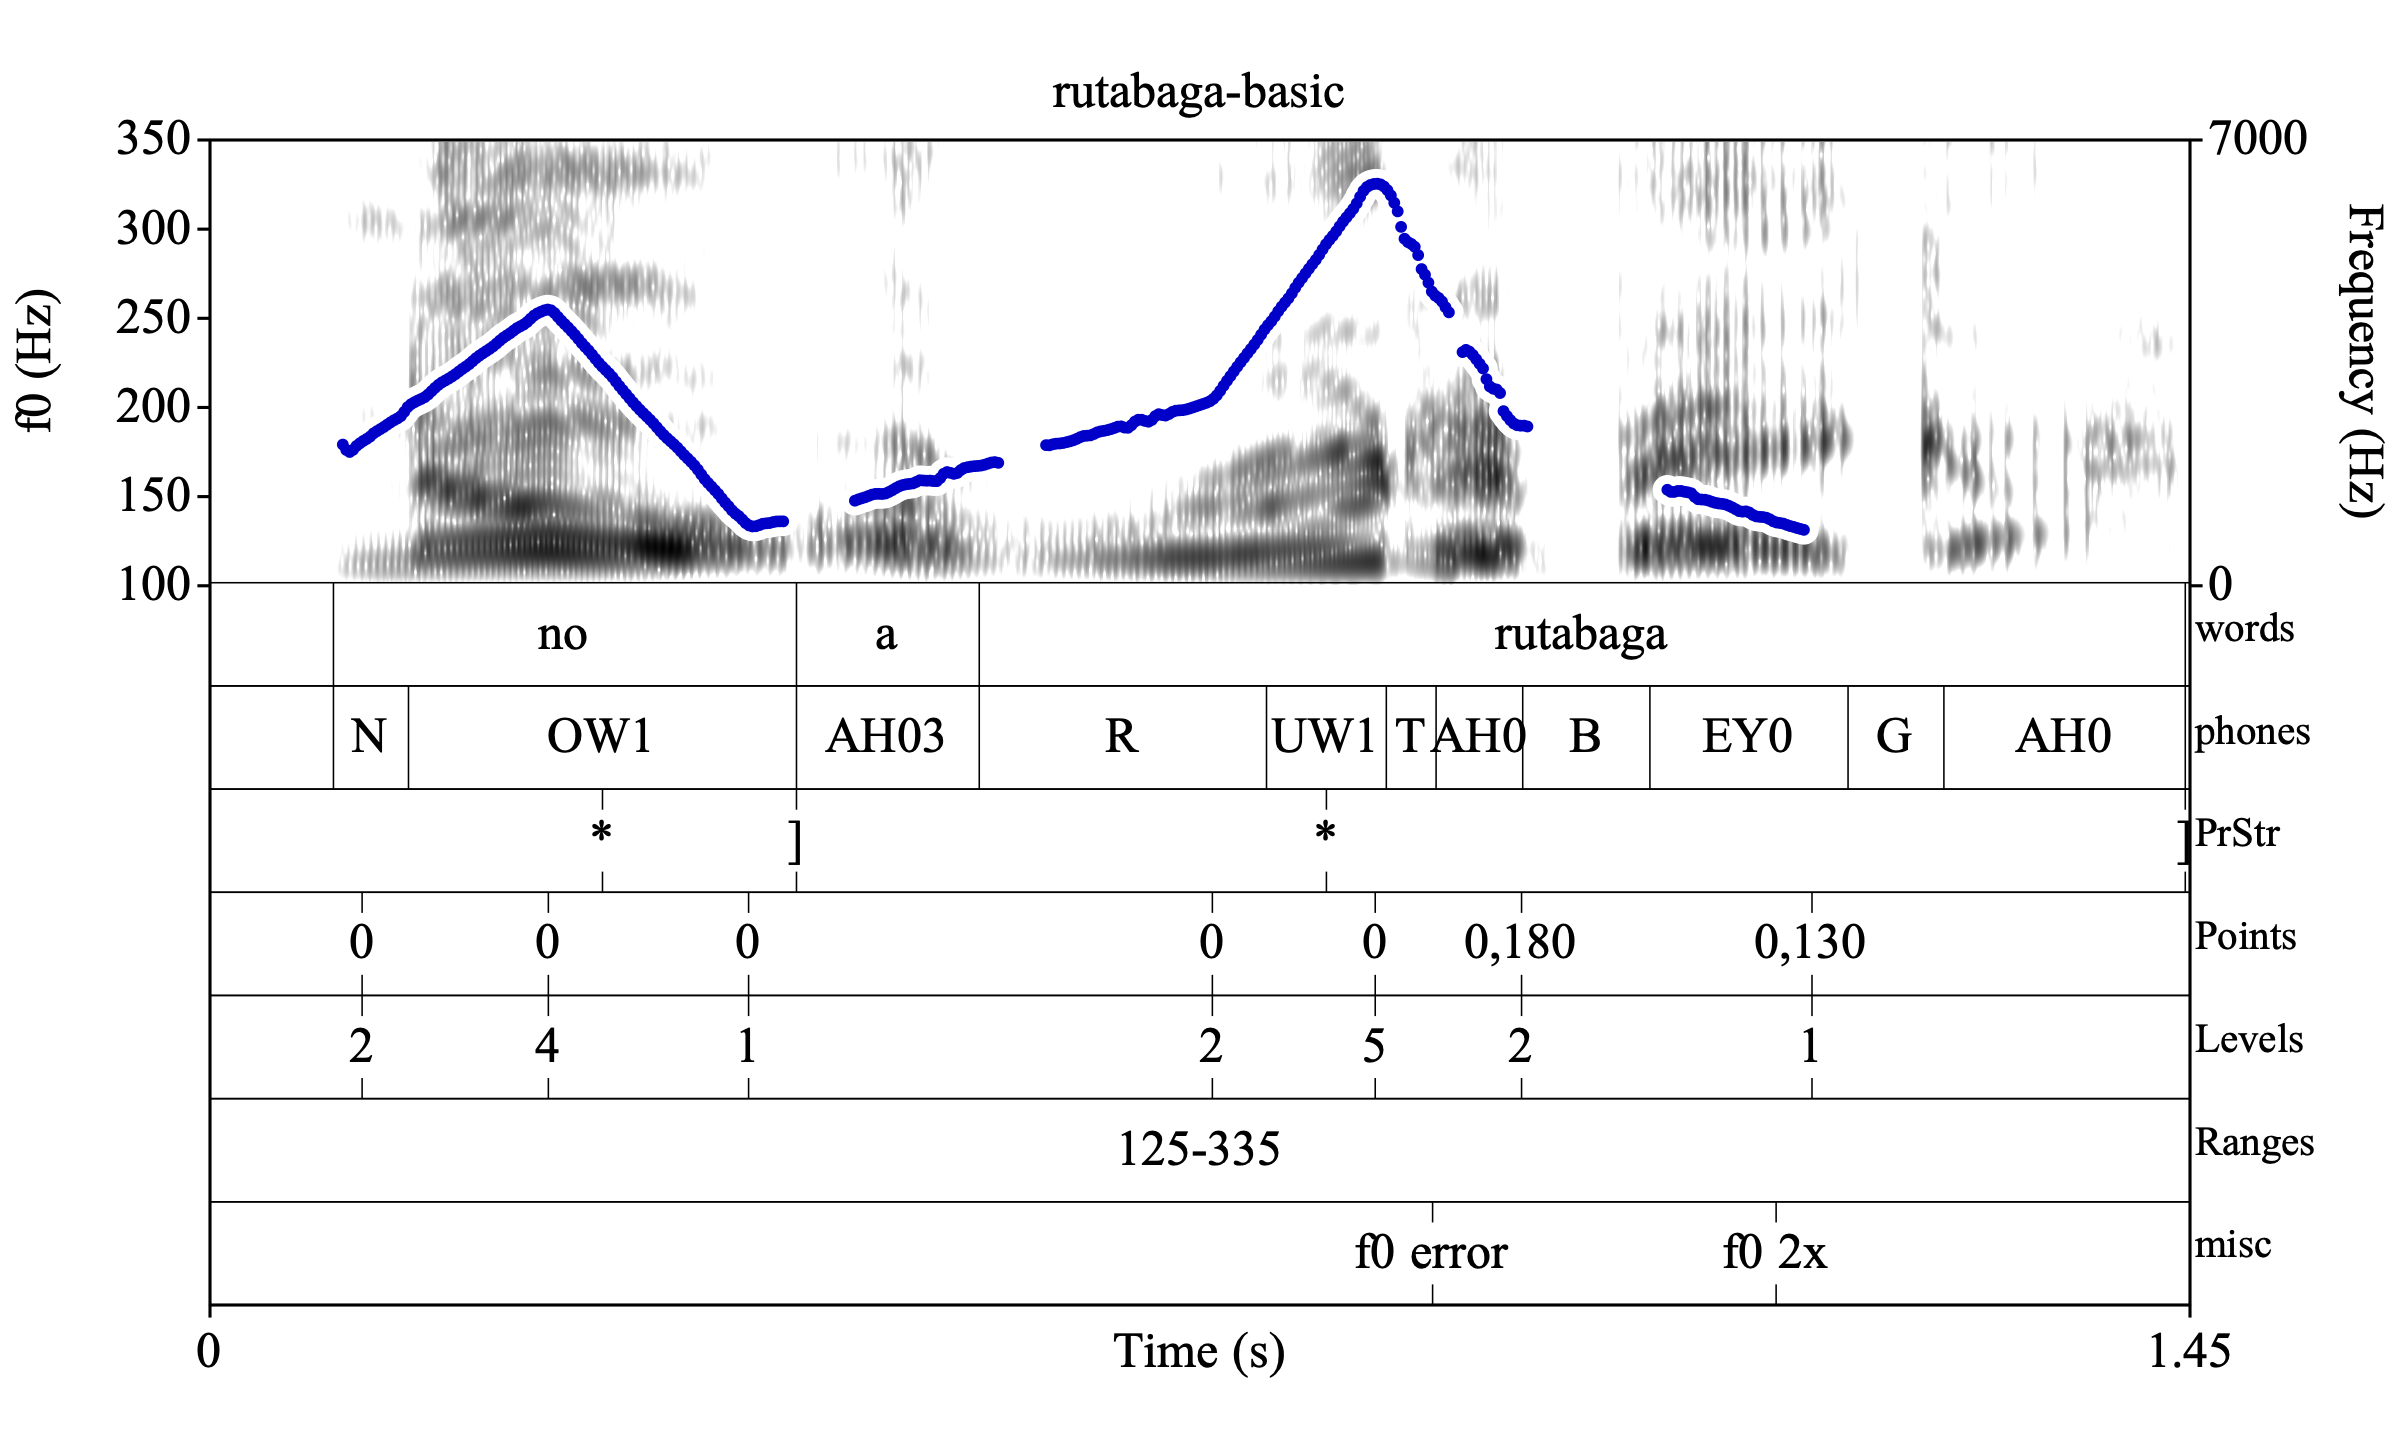
\includegraphics[width=.875\linewidth]{Contours-rutabaga-basic-resynth.png}
%
\caption{A resynthesis that is perceptually equivalent to the original that exhibited pitch doubling.%
\label{fig:rutabaga-resynth f0-tracking}%
\index{Annotated example, f0 tracking!rutabaga}%
}
\end{figure}

In the coming sections, we discuss some common sources of f0 tracking disruptions, that are due to the speech signal itself (and not the software or its settings).

\subsubsection{Segmental effects}\label{sec:segmental-effects}

Another very common set of cases where adjusting software settings may do enough to yield a clean f0 track have to do with the nature of the phonetic characteristics of certain speech sounds. (As noted earlier, these segmental effects are also known as “microprosodic” effects.) Because f0 tracks rely on regular and identifiable repeating patterns in the speech signal, and because speech sounds vary with respect to these properties, the f0 track is frequently influenced by the segments themselves. Some of the core types of segmental effects on f0 tracks are listed here:

\begin{itemize}
\item Voiceless segments: i.e., segments during which there is at least an interval where there is no vocal fold vibration. These are the most straightforward interruptions of the pitch track.
\item Distortions of f0 in the vicinity of obstruents (stops and fricatives): bumps up or down in f0 at the transitions between a consonant and a neighboring segment, or during a voiced fricative
\item Intrinsic pitch of certain vowels: [i] has a higher intrinsic pitch, [a] has a lower one 
\item[] (\uline{HINT}: Sonorant sounds yield fewer segmental effects on pitch, because they involve the most regular and most easily identifiable acoustic patterns with respect to f0.)
\end{itemize}

Consider the example in figure \ref{fig:marmalade cake f0-tracking}, which has the same intonational contour overlaid on utterances with very different segments. The first portion of the recording, “\langtext{Mariana made the marmalade}”, is mostly smooth and steady, because it is primarily composed of sonorant sounds (except the [d] and [ð], where the pitch track is notably less reliable). On the other hand, the second portion of the recording, “\langtext{Jack baked the cake}”, is much less reliable: during the stops and affricates in this utterance, Praat is unable to detect f0. Thus this is an example where the intonational contours are essentially the same, while the f0 tracks are very different, due to segmental effects.

\begin{figure}[H]
\centering
%
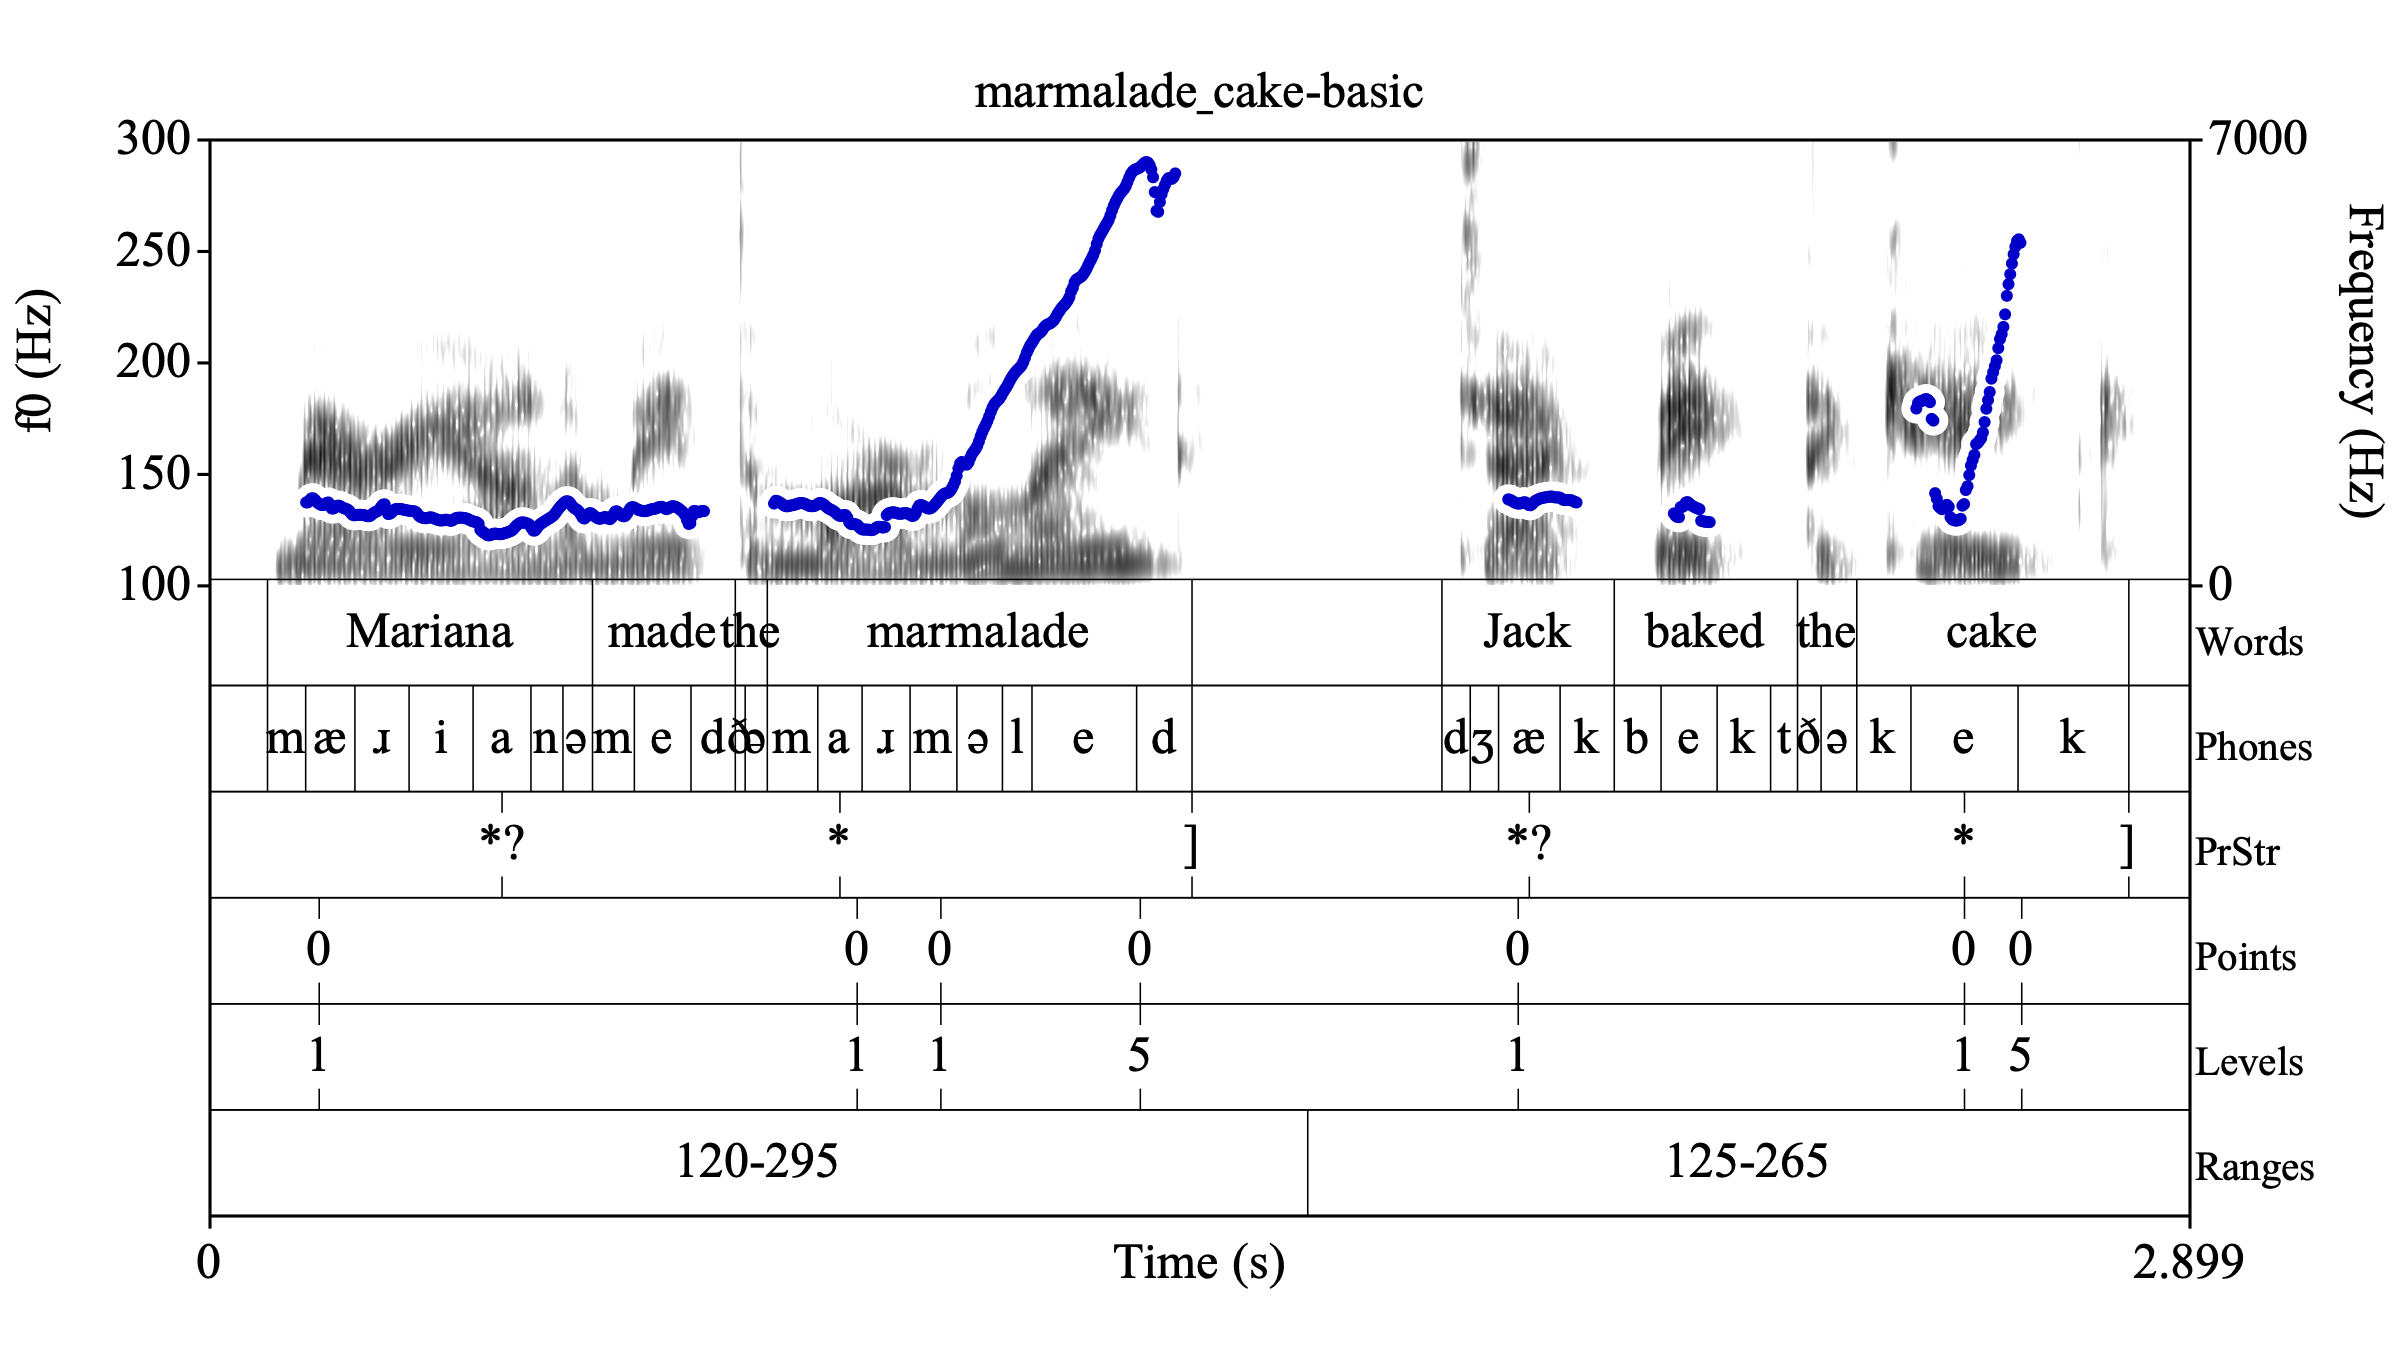
\includegraphics[width=.875\linewidth]{Appendix-marmalade_cake.png}
%
\caption{The same intonational melody applied to a sentence largely comprised of sonorant sounds (left) and to a sentence with many non-sonorants (right).%
\label{fig:marmalade cake f0-tracking}%
\index{Annotated example, f0 tracking!marmalade\_cake}%
}
\end{figure}

The example in figure \ref{fig:design improvements f0-tracking} shows additional examples where the f0 track is heavily distorted by non-sonorant sounds.  In particular, note that the [z] in “\langtext{design}” and the [mp] in “\langtext{improvements}” both cause a significant drops in the f0 track, but they do not correspond to drops in pitch – listening to this example, labellers perceive the pitch as rising steadily from the beginning of “\langtext{design}” to the peak in “\langtext{improvements}”, as reflected by the Points tier labels (which skip over the two mentioned drops in f0).

\begin{figure}[H]
\centering
%
\includegraphics[width=.875\linewidth]{Appendix-design_improvements.png}
%
\caption{An example where non-sonorant sounds disturb the f0 tracking; this is especially noticeable in the [z] of “\langtext{design}” and [p] of “\langtext{improvements}”.%
\label{fig:design improvements f0-tracking}%
\index{Annotated example, f0 tracking!design\_improvements}%
}
\end{figure}

Consider now the example in figure \ref{fig:out of order-plateau f0-tracking}, which exhibits many small rises\slash falls in the f0 track. Note that the Points tier annotations reflect that the annotators perceive the pitch containing many fewer turning points – for example, the Points annotation reflects a mostly steady pitch during “\langtext{seems like it’s}”. This perception of much smoother pitch is reflected in the straight line approximation resynthesis in figure \ref{fig:out of order-plateau f0-tracking}.

\begin{figure}[H]
\centering
%
\includegraphics[width=.875\linewidth]{Appendix-out_of_order-plateau}
%
\caption{An example with lots of perturbations in the f0, due to segmental effects.%
\label{fig:out of order-plateau f0-tracking}%
\index{Annotated example, f0 tracking!out\_of\_order-plateau}%
}
\end{figure}


\begin{figure}[H]
\centering
%
\includegraphics[width=.875\linewidth]{Appendix-out_of_order-plateau-resynth}
%
\caption{A resynthesis on the basis of the Points annotation, to reflect the much smoother intonational contour that the annotator perceives.%
\label{fig:out of order-plateau f0-tracking}%
}
\end{figure}


\subsubsection{Voice quality effects}\label{sec:voice-quality-effects}
In addition to speech segments affecting how f0 is tracked, the voice quality of speech can also impact f0 tracking. (\uline{NOTE}: Voice quality effects —especially from creakiness— are especially common at the edges of prosodic groups.) Voice quality (a.k.a. phonation) refers to how the vocal folds (and the larynx more broadly) are configured during speech production. Modal voice (the “neutral” voice quality) does not impact f0 tracking, while other phonations such as creaky voice, breathy voice, and whisper voice can and do regularly impact f0 tracking. For example, during whispering or breathiness, the f0 track may be absent or values may appear somewhat scattered. 

A particularly frequent non-modal phonation is creaky voice; it is especially common at the ends of phrases and where the pitch is low. It is marked by irregular pitch periods and especially perceptual glottalization (which can be seen in a spectrogram as prominent vertical striations, as during the bulk of the final [i] in Fig. \ref{fig:joey f0-tracking}). During creaky voice, the f0 may disappear or appear to jump suddenly upwards\slash downwards. Both of these effects can be seen in Fig. \ref{fig:joey f0-tracking}: there is creaky voice during “\langtext{it to}” and at the end of “\langtext{Joey}”; during “\langtext{it to}” there is no f0 tracking, and during “\langtext{Joey}”, the f0 tracking jumps suddenly upwards (at the beginning of [i]) and then disappears until the speaker returns to modal voice at the end of the utterance.

\begin{figure}[H]
\centering
%
\includegraphics[width=.875\linewidth]{Appendix-joey.png}
%
\caption{Example of creaky voice phonation disturbing pitch tracking.%
\label{fig:joey f0-tracking}%
\index{Annotated example, f0 tracking!joey}%
}
\end{figure}

Another example of the impact of creaky voice on f0 tracking can be seen in Fig. \ref{fig:no_cigar f0-tracking}. From the beginning of “\langtext{but}” through the [n] of “\langtext{no}”, there is creaky voice during. During that time, there is no pitch tracking (even during the voiced [ʌ] and [n]), and when the f0 tracking returns, it appears to be high and falling onto the [o]; however, this f0 fall is due to the offset of creaky voice, and auditory perception indicates  that the pitch is steadily rising during “but no” (as reflected in Points labels). (Notice also that there are segmental effects from the [s] and [g] of “\langtext{cigar}".)

\begin{figure}[H]
\centering
%
\includegraphics[width=.875\linewidth]{Levels-no_cigar-basic.png}
%
\caption{Example of creaky voice phonation disturbing pitch tracking.%
\label{fig:no_cigar f0-tracking}%
\index{Annotated example, f0 tracking!joey}%
}
\end{figure}


\subsection{Guiding principles for recognizing and dealing with pitch track disruptions}\label{sec:guiding-principles-for-recognizing-and-dealing-with-pitch-track-disruptions}

\begin{enumerate} \def\labelenumi{\arabic{enumi}.}
\item If the f0 appears to change locally in a way that is surprisingly rapid and not clearly part of a bigger pitch pattern, consider the context in which those bumps, spikes or jumps are occurring. Could they be due to segmental effects or pitch tracking errors? Is the “pitch range” in the “pitch settings”
\item In PoLaR labelling, where possible, put Points labels at places in the signal where you believe that the f0 measured corresponds to the pitch you perceive at that region of the utterance
\item For places where you believe a point or range floor or ceiling occurs during unreliable pitch, estimate what the f0 value should be at that point. (See detailed guidelines in the Advanced Points labelling section.) \end{enumerate}




%%%%%%%%%%%%%%%%%%%%%%%%%%%%%%%%%%%%
%%%%
%%%%     CHAPTER 3 advanced
%%%%
%%%%%%%%%%%%%%%%%%%%%%%%%%%%%%%%%%%%
\chapter{PoLaR Guidelines: Advanced Labels}\label{ch:advanced}

A distinct advantage of PoLaR is that labellers can become quite proficient in how to do the “Basic” labels with little in the way of training. This is in large part due to the fact that PoLaR \textit{\uline{does not}} require its labellers to adopt any theory of either how its various labelled characteristics are expected to distribute, or how the characteristics are connected to one another. (This is a departure from other annotation systems, such as those designed to encode contrastive phonological categories.) Thus, a PoLaR labeller need not consider theoretical models or the analytical ramifications of whether to label an aspect of the intonation with a phonological label (or which phonological label to use).

While this design characteristic allows PoLaR labels to be used proficiently (and quickly!) by people who are not working with an eye towards theoretical models, it is still true that many labellers do have theoretical commitments or analyses that they want to encode into their labels. For example, in the example in Figure \ref{fig:to volunteer-halved all basics}, a labeller may wish to annotate that some of the pitch turning points are associated with exponents of a syllable prominence (i.e., prominence-marking) while others are associated with exponents of a phrase boundary (i.e., boundary-marking).

\begin{figure}[H]
\centering
%
\includegraphics[width=.875\linewidth]{Appendix-to_volunteer-halved.png}
%
\caption{\texttt{to\_volunteer-halved}: An example annotated with PoLaR’s Basic labels.%
\label{fig:to volunteer-halved all basics}%
}
\end{figure}

There is no way to annotate this using PoLaR’s Basic labels, but this is the sort of thing the PoLaR Advanced labelling conventions (described in this chapter) have been designed for. Exactly how this and other analytical moves get transcribed using PoLaR Advanced labels will be described in the sections that follow.

While PoLaR Basic labels are designed to elicit agreement (even among labellers with different backgrounds in prosodic theory), Advanced labels may require labellers to have shared theoretical\slash analytical priors, in order for agreement to be reached. The PoLaR annotation system itself is not designed to provide answers that can adjudicate in these discussions, but rather it is meant to provide a starting point for these discussions to take place.

Before moving on, let us be clear about the optionality of using PoLaR Advanced labels. As described briefly above, PoLaR Advanced labels serve as a means to systematically encode higher levels of analysis or deeper intuitions that the labeller wishes to commit to. While other annotation systems require such higher-level commitments in most\slash all of their labels, PoLaR Advanced labels are always opt-in. This means that in cases where the labeller does not wish to commit to a particular analysis, they are not required to do so. (In sum, mixing PoLaR Basic labels with Advanced labels is both expected and encouraged, and researchers are encouraged to adopt the (sub)set of Advanced labels that best fits their research goals.)

\section{PoLaR Advanced Labels}\label{sec:polar-advanced-labels}

The sections that follow describe what we call PoLaR Advanced labels. These labels occupy the same four core PoLaR tiers (PrStr, Points, Levels, Ranges), but can encode more of the analyses and intuitions of advanced labellers, allowing for the annotation of relationships across tiers and for the inclusion of ideas informed by prosodic theories. In addition, these labels may be especially useful for describing data beyond idealized forms of mainstream varieties of a language produced in a laboratory setting.

Because these labels allow for inclusion of particular analyses, this chapter will have more discussion of how PoLaR labels can connect with prosodic theories and phonological analyses, and also how PoLaR fits in with / compares to existing annotation systems, especially those in the AM tradition. (See also \citealt{ahn-19}.)

A note before introducing these new PoLaR labels: Even with the addition of Advanced labels, these guidelines will \uline{not} provide an exhaustive set of labels that could be used in PoLaR. Labellers are encouraged to take advantage of PoLaR’s flexibility, by augmenting or changing the labels to fit their needs\slash views. However, whenever labellers do deviate from the descriptions set out in these guidelines, they need to provide a document that defines the labels they do use, providing descriptions that are at least as clear as those found in these guidelines (preferably with figures showing examples), so that other users have an explicit understanding of how those labels work.

\section{PrStr (Advanced)}\label{sec:prstr-advanced}

In the PrStr tier, phonological objects related to prominence and phrasing are annotated. In the Basic set of labels, the relevant labels are \textlabel{*} and \textlabel{]} (and their “uncertain” partners, \textlabel{?*} and \textlabel{?]}). One of the ideas behind reducing the number of necessary labels to \textlabel{*} and \textlabel{]} is to simplify the labelling process, allowing even untrained native speakers to provide such labels, in the spirit of Cole’s Rapid Prosody Transcription (\citealt{cole-14}). At the same time, it may be desirable (depending on the demands of the research at hand, and the abilities of the labeller(s)) to provide more detailed intuitions, beyond simply indicating the existence of prominence and phrase boundaries. To serve this need, this section will provide an expanded set of labels for the Prosodic Structure tier, for those who wish to include additional information about prominence and phrasing.

\subsection{Advanced Phrasing Labels}\label{sec:advanced-phrasing-labels}

A key component of any prosodic analysis is an understanding that there are a number of levels of hierarchical structure. English is commonly thought to make use of two phonologically distinct categories of prosodic phrasing (e.g., \citealt{selkirk81}, \citealt{beckmanpierrehumbert86}, \citealt{nesporvogel86}, \textit{et seqq}.), with evidence for such a distinction being rooted in different sorts of boundary phenomena (having to do with pitch movements, speech rate, pauses, pitch reset, etc.; \citealt{brugos-19}). As such, an advanced labeller may wish to distinguish some phrase boundaries from other phrase boundaries that are stronger. Thus in addition to the default \textlabel{]} label, PoLaR provides the \textlabel{]]} label for phrase boundaries that are perceived as stronger than others.

\begin{figure}[H]
\centering
%
\includegraphics[width=.875\linewidth]{PrStr-educate_yourself-adv.png}
%
\caption{The labeller hears the phrase boundary between “\langtext{obvious}” and “\langtext{educate}” as stronger than the phrase boundary between “\langtext{first}” and “\langtext{seems}”.%
\label{fig:educate yourself PrStr Adv}%
\index{Annotated example, PrStr tier (advanced)!educate\_yourself}
}
\end{figure}

PoLaR does not require the labeller to adhere to any particular rigorous definitions for different sorts of prosodic phrases, across recordings. It may simply be that a labeller wishes to distinguish different levels of phrase-sizes in a particular example (perhaps due to their intuitive perception of disjuncture, or perhaps because some acoustic cue such as length of pause is particularly strong). Though labellers need not adhere to any particular rules on when to use \textlabel{]} versus {]]}, labellers may find it helpful to annotate in a “misc” tier what makes a \textlabel{]]} phrase boundary stand out as especially perceptually strong.

\subsubsection{Phrase-Initial Boundaries}\label{sec:phrase-initial-boundaries}

In addition to different sorts of phrase-final boundaries, a labeller may wish to also label the left edges of phrases, by using parallel labels like \textlabel{[}, \textlabel{?[}, and \textlabel{[[}. This may be useful if operating under an approach in which not every right edge of an intonation phrase entails the left edge of another intonation phrase. Because the Strict Layer Hypothesis (cf. \citealt{nesporvogel86}) in effect \textit{prohibits} recursion in prosodic structure, annotating a right edge is essentially annotating a left edge. However, many strands of contemporary research \textit{allow} recursion in prosodic structure (e.g., \citealt{ladd08}, \citealt{selkirk11}, \citealt{itomester12}, and \citealt{kentnerfery13}), making it useful to annotate both left and right edges of a phrase. For example, in a case of center-embedding like in “\langtext{I saw the lion \uline{which he loves} in the toy box}” with the non-restrictive relative clause, some may analyze the phrasing as “(\langtext{I saw the lion} (\langtext{which he loves}) \langtext{in the toy box})” – i.e., there is a phrase-initial edge before \langtext{which} but no phrase-final edge after \langtext{lion}. This could be annotated using Advanced phrasing labels as in Figure \ref{fig:lion toy box PrStr Adv}.

\begin{figure}[H]
\centering
%
\includegraphics[width=.875\linewidth]{PrStr-lion_toy_box-adv.png}
%
\caption{The labeller is annotating an analysis in which “\langtext{lion}” is not phrase-final, even though “\langtext{which}” is phrase-initial.%
\label{fig:lion toy box PrStr Adv}%
\index{Annotated example, PrStr tier (advanced)!lion\_toy\_box}
}
\end{figure}

Similarly, with parentheticals that are produced like “\langtext{I think}” in Figure \ref{fig:long-story-ranges PrStr Adv}, there are cues to “\langtext{I}” being phrase-initial (glottalization), but not many cues to “\langtext{selling}” being phrase final. This could be analyzed in terms of nested prosodic phrases, and such an analysis is labelled on the PrStr tier in that figure.

\begin{figure}[H]
\centering
%
\includegraphics[width=.875\linewidth]{PrStr-long-story-ranges-adv.png}
%
\caption{The labeller is annotating an analysis in which “\langtext{selling}” is not phrase-final, just because “\langtext{I}” is phrase-initial.%
\label{fig:long-story-ranges PrStr Adv}%
\index{Annotated example, PrStr tier (advanced)!long-story-ranges}
}
\end{figure}

For researchers who choose to label phrase beginnings with the \textlabel{[} label, there may be occasions where a single word boundary coincides with both the end of one phrase and the beginning of another, with no intervening silent interval. It is possible to use \textlabel{][} at such points, as is illustrated in Figure \ref{fig:vegetable_list PrStr Adv} below:

\begin{figure}[H]
\centering
%
\includegraphics[width=.875\linewidth]{PrStr-vegetable_list-adv.png}
%
\caption[The labeller has annotated the beginning of each phrase as well as its end.]{The labeller has annotated the beginning of each phrase as well as its end, including an instance of the same location being both a phrase end and a phrase beginning, i.e. the marker between “\langtext{beans}” and “\langtext{some}.”%
\label{fig:vegetable_list PrStr Adv}%
\index{Annotated example, PrStr tier (advanced)!vegetable\_list}
}
\end{figure}

Note that we offer this \textlabel{[} label as a tool for those who would find using it to be helpful for their research purposes, and using it is by no means required. In other words, use the \textlabel{[} label if you are compelled to, but we take no stance on how often labellers should be using it (if at all). For some cases where \textlabel{[} labels may be useful for Advanced Points labels, see section \ref{sec:points-associated-with-phrase-initial-boundaries}.

\subsubsection{Summary of Phrasing Labels}\label{sec:summary-of-phrasing-labels}

Basic labels are highlighted, to be used by all, with the remaining Advanced labels provided for labellers who have more experience or who are targeting particular phenomena. As a reminder: phrasing is cued by acoustics, but these labels are about the labeller’s \textit{perception} or phrasing, in the given utterance context.

\begin{longtable}{clp{.5\linewidth}} \toprule \textbf{Label} & \textbf{Phonological Object} & \textbf{Significance of Label}\tabularnewline
\midrule \endhead
\rowcolor{green}
\textlabel{]} & Prosodic Phrase Boundary & A prosodic phrase ends at this point \tabularnewline
\textlabel{?]} & Possible Prosodic Phrase Boundary & A prosodic phrase may end at this point, but the labeller is uncertain \tabularnewline
\textlabel{]]} & Large Prosodic Phrase Boundary & A noticeably large prosodic phrase ends at this point \tabularnewline
\textlabel{[} & Prosodic Phrase Boundary & A prosodic phrase begins at this point \tabularnewline
\textlabel{?[} & Possible Prosodic Phrase Boundary & A prosodic phrase may begin at this point, but the labeller is uncertain \tabularnewline
\textlabel{[[} & Large Prosodic Phrase Boundary & A noticeably large prosodic phrase begins at this point \tabularnewline
%
\bottomrule
\caption{Advanced PrStr phrasing labels: encoding uncertainty or boundary strength.}
\end{longtable}

\subsection{Advanced Prominence Labels}\label{sec:advanced-prominence-labels}

Just as there are levels of prosodic phrasing, in some cases different levels of prosodic prominence can be identified perceptually and/or acoustically. In such cases an advanced labeller may wish to distinguish some prominences from other prominences that are stronger. Thus in addition to the default \textlabel{*} label, PoLaR provides the \textlabel{**} label for prominences that are perceived as stronger than others.

\begin{figure}[H]
\centering
%
\includegraphics[width=.875\linewidth]{PrStr-naomi_email-adv.png}
%
\caption{The labeller is annotating the perception that “\langtext{Naomi}” and “\langtext{email}” are both prominent, but that “\langtext{Naomi}” is significantly more prominent.%
\label{fig:naomi_email PrStr Adv}%
\index{Annotated example, PrStr tier (advanced)!naomi\_email}
}
\end{figure}


As with all Advanced labels, there is no need to use \textlabel{**} in every utterance. As default guidance for distinguishing \textlabel{*} and \textlabel{**}, labellers should only use the \textlabel{**} label when it is very clear that one of the prominences is perceived as especially strong, as compared to the other words in the context of the utterance.

Additionally, as with the \textlabel{]} and \textlabel{]]} labels, PoLaR does not require the labeller to adhere to any particular rigorous definitions for different sorts of prominence across their entire corpus; a labeller may simply wish to distinguish different degrees of prominence in a given example (perhaps as a simple matter of perceptual strength, perhaps because of especially high f0 peaks, etc.). That said, labellers are encouraged to annotate in a “misc” tier what makes a \textlabel{**} prominence stand out as especially perceptually strong.

\subsubsection{Summary of Prominence Labels}\label{sec:summary-of-prominence-labels}

Basic labels are highlighted, to be used by all, with the remaining labels proposed for labellers who have more experience or who are targeting particular phenomena. As a reminder: prominence is cued by acoustics, but these labels are about the labeller’s \textit{perception} or prominence, in the given utterance context.

\begin{longtable}{clp{.5\linewidth}} \toprule \textbf{Label} & \textbf{Phonological Object} & \textbf{Significance of Label}\tabularnewline
\midrule \endhead
\rowcolor{green}
\textlabel{*} & Prominence & The constituent this occurs in is prominent\tabularnewline
\textlabel{?*} & Possible Prominence & The constituent this occurs in might be prominent, but the labeller is uncertain \tabularnewline
\textlabel{**} & Especially Strong Prominence & The constituent this occurs in is especially prominent \tabularnewline
%
\bottomrule
\caption{Advanced PrStr prominence labels: encoding uncertainty or prominence strength.}
\end{longtable}

\subsection{Disfluency}\label{sec:disfluency}

Here we pivot from labelling phrasing and prominence to labelling a phenomenon that may interact with perceived phrasing\slash prominence: disfluencies in speech. A disfluency is defined here as a disruption of fluent, connected speech, which manifests acoustically as a change in speech rate, a change in pitch trajectory, addition of a pause, etc. Such an acoustic disruption can be momentary in nature, or it can be observed over a period of time. (See \citealt{shattuck-hufnagelcutler99} for a discussion of how different types of disfluency can be marked prosodically. In addition, \citealt{brugos-19} describes in more detail the range of disfluency effects on prosody that are attested in English.) Characteristic of all types of disfluencies is that, if a speaker were to repeat an idealized form of the disfluency-containing utterance, with the same intended meaning, the idealized repetition could lack all disfluent regions.

As disfluencies can influence prosody in measurable ways, a labeller may find it useful to label disfluent speech as such. For this purpose, PoLaR provides the ‘\textlabel{d}’ label, which is to be marked on the PrStr tier, at the point in the utterance where there is a disfluency: i.e., in the word or partial word (in the case of a cut-off word) where the disfluency is noticed.

While disfluencies may differ prosodically from one another, this ‘d’ label can be used for all types. An example of a disfluency that corresponds to a momentary stutter (with no sense of disjuncture) is given in Figure \ref{fig:in_a_plane-disfluencies PrStr Adv}. Additionally, an example of a disfluency that induces a sense of disjuncture like that of a phrase boundary (due to the overlap in set of cues) is given in Figure \ref{fig:spoon_here PrStr Adv}. In both cases, the ‘\textlabel{d}’ label is on the PrStr tier, time-aligned with the onset of the disfluent moment\slash region, or where the speaker cuts themselves off.

\begin{figure}[H]
\centering
%
\includegraphics[width=.875\linewidth]{PrStr-in_a_plane-disfluencies-adv.png}
%
\caption[\texttt{in\_a\_plane-disfluencies}, with Advanced PoLaR labels.]{\texttt{in\_a\_plane-disfluencies}, with Advanced PoLaR labels. Note the ‘d’ on PrStr, annotating at the cut-off, before a restart begins.%
\label{fig:in_a_plane-disfluencies PrStr Adv}%
\index{Annotated example, PrStr tier (advanced)!in\_a\_plane-disfluencies}
}
\end{figure}

\begin{figure}[H]
\centering
%
\includegraphics[width=.875\linewidth]{PrStr-in_a_plane-disfluencies-adv.png}
%
\caption[\texttt{spoon\_here}, with Advanced PoLaR labels. Note the ‘\textlabel{d}’ on PrStr.]{\texttt{spoon\_here}, with Advanced PoLaR labels. Note the ‘\textlabel{d}’ on PrStr, annotating where a labeller may perceive some of the prosody associated with this disfluency as cues to phrase break.%
\label{fig:spoon_here PrStr Adv}%
\index{Annotated example, PrStr tier (advanced)!spoon\_here}
}
\end{figure}

There may be cases in which a speaker produces not just a single disfluency, but a disfluent region. For such cases, the labeller can designate the beginning and ending of such a region by using the ‘\textlabel{\{d}’ and ‘\textlabel{d\}}’ labels in the PrStr tier at the beginning and end (respectively) of this region. The labeller can choose to skip over other labelling decisions within this designated region. Such an example is shown in Figure \ref{fig:experience-disfluent-region PrStr Adv}.

\begin{figure}[H]
\centering
%
\includegraphics[width=.875\linewidth]{PrStr-experience-disfluent-region.png}
%
\caption[\texttt{experience}, with Advanced PoLaR labels. Note the region flanked by ‘\textlabel{\{d}’ and ‘\textlabel{d\}}’ on PrStr.]{\texttt{experience}, with Advanced PoLaR labels. Note the region flanked by ‘\textlabel{\{d}’ and ‘\textlabel{d\}}’ on PrStr, which annotate a stretch of time that sounds disfluent.%
\label{fig:experience-disfluent-region PrStr Adv}%
\index{Annotated example, PrStr tier (advanced)!experience}
}
\end{figure}

In all cases, the ‘\textlabel{d}’ label of PoLaR allows the labeller to annotate the presence of one or more disfluencies, without any information about the acoustic details or which (if any) type of speech error it corresponds to. Labellers who wish to label more about the details of the disfluency are encouraged to use a system of labels designed to annotate this information, perhaps on a different tier. (See \citealt{brugos-19} for some ideas of disfluency labels that could work alongside PoLaR.)

\begin{longtable}{cp{.3\linewidth}p{.45\linewidth}}
	\toprule
	\textbf{Label} & \textbf{Phonological Object} & \textbf{Time-Aligned with} \tabularnewline
	\midrule
	\endhead
	\textlabel{d} & Disfluency & A point in the utterance where there is a disfluency\tabularnewline
	\textlabel{\{d} & Start of a disfluent region & A point in the utterance where a disfluent region of speech begins\tabularnewline
	\textlabel{d\}} & End of a disfluent region & A point in the utterance where a disfluent region of speech ends\tabularnewline
	\bottomrule
	\caption{Advanced PrStr labels: encoding disfluency.}
\end{longtable}


\subsection{Examples with Advanced PrStr labels}\label{sec:examples-with-advanced-prstr-labels}

In this section we have reviewed some ways to systematically label these more refined intuitions, beyond the simple contrast of presence\slash absence of \textlabel{*} and \textlabel{]} labels; e.g., using the contrast between \textlabel{*} and \textlabel{**} labels, and \textlabel{]} and \textlabel{]]} labels to differentiate degrees of prominence\slash phrasing. In addition to the examples provided earlier in this section, these more fine-grained contrasts are exemplified in Figure \ref{fig:out_of_order_huh PrStr Adv} and Figure \ref{fig:asked_only_an_illusion PrStr Adv}.

\begin{figure}[H]
\centering
%
\includegraphics[width=.875\linewidth]{PrStr-out_of_order_huh-adv.png}
%
\caption[The labeller hears especially strong breaks after “\langtext{huh}” and after “\langtext{again}”.]{The labeller hears especially strong breaks after “\langtext{huh}” and after “\langtext{again}”; they also hear especially strong prominence on “\langtext{order}”.%
\label{fig:out_of_order_huh PrStr Adv}%
\index{Annotated example, PrStr tier (advanced)!out\_of\_order\_huh}
}
\end{figure}

\begin{figure}[H]
\centering
%
\includegraphics[width=.875\linewidth]{PrStr-asked_only_an_illusion-adv.png}
%
\caption[The labeller is at several points uncertain about prominence.]{The labeller is at several points uncertain about prominence (“\langtext{she}”, “\langtext{believes}”, “\langtext{only}”), while also hearing especially strong prominence on “\langtext{illusion}” and especially strong phrase boundaries after “\langtext{still}” and “\langtext{illusion}”.%
\label{fig:asked_only_an_illusion PrStr Adv}%
\index{Annotated example, PrStr tier (advanced)!asked\_only\_an\_illusion}
}
\end{figure}

The following example Figure \ref{fig:at_this_point-disfluencies PrStr Adv} includes instances of both labeller uncertainty about prominence (\textlabel{?*}) and a perceived a disfluency (marked with the ‘\textlabel{d}’ label). Note that some disfluencies have pauses immediately following and some do not; if it feels like the disfluency leads to new prosodic phrase boundaries, these boundaries should be annotated separately. (Likewise for disfluency-induced prominence.)

\begin{figure}[H]
\centering
%
\includegraphics[width=.875\linewidth]{PrStr-at_this_point-disfluencies-adv.png}
%
\caption[The labeller hears several disfluencies.]{The labeller hears several disfluencies, where the speaker restarts\slash recasts their speech; the ‘\textlabel{d}’ labels that indicate this are at the cut-off point, before any existing disfluency-related pauses.%
\label{fig:at_this_point-disfluencies PrStr Adv}%
\index{Annotated example, PrStr tier (advanced)!at\_this\_point-disfluencies}
}
\end{figure}

\subsection{Summary of the Advanced Labels for the PrStr Tier}
This section has reviewed the Advanced labels set out for transcription in the PrStr tier. As with all Advanced labels described in this chapter, their significance and guidelines for usage are provided here, but none of the Advanced labels are required for PoLaR labellers. For example, as mentioned for the phrase-initial boundary label, \textlabel{[}, some labellers might want to use this label, while others may use it infrequently, or not at all. Similar can be said for the \textlabel{**} and disfluency-related labels.

The exhaustive list of Advanced PrStr labels are laid out in the table below, which compiles the tables found throughout this section.

\begin{longtable}{cp{.3\linewidth}p{.45\linewidth}}
	\toprule
	\textbf{Label} & \textbf{Phonological Object} & \textbf{Time-Aligned with} \tabularnewline
	\midrule
	\endhead
	\rowcolor{green}
	\textlabel{]} & Prosodic Phrase Boundary & The end of a Words interval where a prosodic phrase ends \tabularnewline
	\textlabel{?]} & Possible Prosodic Phrase Boundary & The end of a Words interval where a prosodic phrase may end (but the labeller is uncertain) \tabularnewline
	\textlabel{]]} & Large Prosodic Phrase Boundary & The end of a Words interval where a noticeably large prosodic phrase ends \tabularnewline
	\textlabel{[} & Prosodic Phrase Boundary & The beginning of a Words interval where a prosodic phrase begins \tabularnewline
	\textlabel{?[} & Possible Prosodic Phrase Boundary & The beginning of a Words interval where a prosodic phrase may begin (but the labeller is uncertain) \tabularnewline
	\textlabel{[[} & Large Prosodic Phrase Boundary & The beginning of a Words interval where a noticeably large prosodic phrase \tabularnewline
	\hline
	\rowcolor{green}
	\textlabel{*} & Prominence & The center of the Phones/Words interval that is prominent\tabularnewline
	\textlabel{?*} & Possible Prominence & The center of the Phones/Words interval that might be prominent (but the labeller is uncertain) \tabularnewline
	\textlabel{**} & Especially Strong Prominence & The center of the Phones/Words interval that is especially prominent \tabularnewline
	\hline
	\textlabel{d} & Disfluency & A point in the utterance where there is a disfluency\tabularnewline
	\textlabel{\{d} & Start of a disfluent region & A point in the utterance where a disfluent region of speech begins\tabularnewline
	\textlabel{d\}} & End of a disfluent region & A point in the utterance where a disfluent region of speech ends\tabularnewline
	\bottomrule
	\caption{The PrStr labels described in this chapter, which can be used by Advanced PoLaR labellers.}
\end{longtable}


\section{Points (Advanced)}\label{sec:points-advanced}

\subsection{Optional Advanced Labels for Relating Objects on Points Tier to Objects on Prosodic Structure Tier}\label{sec:optional-advanced-labels-for-relating-points-tier-objects-to-prosodic-structure-tier-objects}

One valuable aspect of the PoLaR system is that it allows labellers to annotate aspects of the intonational phonetics (e.g., time alignment of turning points) separately from aspects of the intonational phonology (e.g., prominences or boundaries). This independence can be achieved through using ‘\textlabel{0}’ labels on the Points tier, as we described for Basic Points labels in Chapter \ref{ch:basics}. These PoLaR Basic labels (consisting of ‘\textlabel{0}’ labels and optional comma-overrides) can be revised in a second-pass of labelling: in the first pass, PoLaR Basic Prosodic Structure and Points tiers are labelled, and in the second pass, ‘\textlabel{0}’ labels are replaced with more complex labels (described in this section) to capture relationships between the  labels on the Points tier with those on the PrStr tier. To understand these complex labels, we describe first what such labels are designed to capture, before going into the details of how to use them.

It is commonly understood that some pitch movements (like those annotated on the Points tier) are associated with (i.e., manifest cues to) particular prosodic events (like those annotated on PrStr). For example, some pitch movements are used to mark prominences, while others are used to mark boundaries. The labeller, therefore, might ask themselves if a particular turning point contributes to an intonational contours’s shape that in turn contributes to a listener’s perception of prominence or phrasing. In cases where the answer is ‘yes’, the Advanced Points labels provide the means for the labeller to capture this relationship.

Even relatively naive intonational annotators will note that pitch patterns often serve as acoustic cues to a prominence or phrase boundary. Consider the example in Figure \ref{fig:amelia_knew2 in Adv}, annotated with Basic PoLaR labels.

\begin{figure}[H]
\centering
%
\includegraphics[width=.875\linewidth]{Points-amelia_knew2.png}
%
\caption{\texttt{amelia\_knew2}, with Basic PoLaR labels.%
\label{fig:amelia_knew2 in Adv}%
\index{Annotated example, PrStr tier (advanced)!at\_this\_point-disfluencies}
}
\end{figure}

Here the third label on the Points tier (marking the f0 peak) is cueing the prominence on “\langtext{Amelia}” labelled on the PrStr tier, while the final two labels on the Points tier (marking the phrase-final rise) cue the utterance-final phrase boundary labelled on the PrStr tier. Which, if any, of the other Points labels are related to the PrStr objects is subject to some debate, and labellers may well disagree.

Users of other annotation systems are intimately familiar with this idea; much of what many other annotation systems do is model the relationship between pitch movements and other prosodic objects. Systems that do this include those that make an important distinction between pitch movements of various types; e.g., IPO, ToBI, IViE, or RaP. Because of this, such labellers have strong intuitions whether a particular f0 turning point “belongs to” a prominence (i.e., manifests a cue for a pitch accent) or a phrase boundary (i.e., manifests a cue for an edge tone). PoLaR labellers who are familiar with those models are encouraged to use their background in these other models to inform how they relate Points and PrStr objects with Advanced Points labels. (Note this means users with different theoretical priors may well label the same Basic Points labels of a single utterance with different Advanced Points labels - we take this to be a feature, not a bug.)

Below we provide a more comprehensive description of the Advanced PoLaR labels that can replace pitch turning points that are originally marked with a ‘\textlabel{0}’ on the Points tier, to indicate that a given turning point is perceived to be prominence-marking or edge-marking (or both). A PoLaR Advanced Points label consists of a minimum of two components: (i) the \textit{\uline{type}} of phonological object the turning point is associated with, and (ii) a \textit{\uline{pointer}} to the relevant Prosodic Structure tier label’s time coordinate. We find that there are three different scenarios that arise when deciding whether a turning point is associated with a prosodic event labelled on the PrStr tier, and if so, with which one:

\begin{enumerate} \def\labelenumi{\arabic{enumi}.}
\item No PrStr labelled event is associated with the f0 turning point, or it’s not clear that one is. In this case, use ‘\textlabel{0}’ as the complete label. (This is a ‘neutral’ label, indicating that the labeller is not committing to any particular analysis, but has determined that a significant turning point needs to be marked at that location.)
\item A particular \textit{\uline{type}} of PrStr labelled event (either ‘\textlabel{*}’ or ‘\textlabel{]}’; marked below as ‘\textlabel{\_}’) is associated with the f0 turning point, which is time-aligned in various ways, indicated by one of three \textit{\uline{pointer}}s:

 \begin{enumerate} \def\labelenumii{\alph{enumii}.}
\item PrStr label follows Points label (‘\textlabel{\_>}’)
\item PrStr label precedes Points label (‘\textlabel{\_<}’)
\item {[\textit{uncommon}]} PrStr label is precisely co-timed with Points label (‘\textlabel{\_@}’) \end{enumerate}
\item Occasionally, multiple PrStr labelled events are associated with a single f0 turning point. That is, the turning point is either (i) ambiguous between being associated with the preceding PrStr labelled event and being associated with the following event, or (ii) the labeller believes that the point relates to both of those events. In these cases a complex label is used, with two labels separated by a \textlabel{/} (‘\textlabel{\_</\_>}’). \end{enumerate}

There are two observations to be made about these labels right away. First, any non-‘\textlabel{0}’ label on the Points tier indicates the labeller has an intuition about the appropriate analysis. Thus, in the absence of such an intuition, the advanced labeller should leave the ‘\textlabel{0}’ label in place.

Second, the pointers themselves (‘\textlabel{>}’, ‘\textlabel{<}’, ‘\textlabel{@}’) carry no significance beyond indicating a relationship of how a PrStr label and a Points label happen to be time-aligned. That is, because the timing of a PrStr label is at the discretion of the labeller, its precise location in time is not meaningful.  Thus, a label ‘\textlabel{*>}’ in the Points tier simply means that “this turning point manifests a cue to the prominence labelled as a ‘\textlabel{*}’ on the Prosodic Structure tier, which is time-aligned later than (to the right of) this Points tier label.” A minimally different label, ‘\textlabel{*<}’, says that the relevant PrStr ‘\textlabel{*}’ label is time-aligned earlier than the Points tier label. To repeat, in the interest of clarity: these two labels are not in and of themselves informatively different, in part because the particular timing of the PrStr label is not informative.\footnote{In other words, the difference between, e.g., ‘\textlabel{*>}’ and ‘\textlabel{*<}’ is not a meaningful one; it may simply be a reflection of how the ‘\textlabel{*}’ label happens to be timed – which is at the whim of the labeller. (Recall that the ‘\textlabel{*}’ label on the PrStr tier need only be time-aligned within the stressed vowel.) This may be somewhat surprising for labellers familiar with other annotation systems, where labels that use different symbols in a label are meant to signify meaningful\slash phonological distinctions (e.g., \textlabel{L+H*} vs. \textlabel{L*+H} in ToBI or \textlabel{H*L} vs. \textlabel{!H*L} in IViE).}

The options and the order of the notation is summarized below. (A more complete grammar for Points tier labels is provided in section \ref{sec:summary-of-the-points-tier}.)

\begin{figure}[H]
\centering
%
  \begin{tikzpicture}[node distance=4em, anchor=west, align=flush center, FLOW/.style={->, very thick}, LABEL/.style={draw, fill=yellow!80, inner sep=.75em}, scale = .775, transform shape]
    \node[draw, text width=5.5em] (node2) {Assert a relationship to a PrStr object?};
    \node[LABEL, below right=1em and 6em of node2.east] (node3no) {\textlabel{0}};
    \node[LABEL, above right=1em and 6em of node2.east] (node3yes) {\textlabel{*}\\\textlabel{]}\\\textlabel{[}};
    \node[draw, text width=8em, right=3em of node3yes] (node4) {Where is the PrStr Tier object that corresponds to the Points Tier object?};
    \node[LABEL, right=3em of node4.east] (node5) {\textlabel{>}\\\textlabel{<}\\\textlabel{@}};
    \node[draw, text width=8em, below=1.5em of node5, anchor=north] (node6) {Could this Points Tier object also correspond to another PrStr object?};
    \node[right=3em of node6] (node7yes) {};
    \node[LABEL, above=of node7yes.center] (node7) {\textlabel{/}};
    \node[above=5em of node7] (node7-loopback1) {};
    \node[above=2em of node3yes] (node7-loopback2) {};
%%%%%%%%%%%%%%%
%%%%%%%%%%%%%%%
    \draw [black,FLOW] (node2.east) -- node[pos=0.5, above, sloped]{Yes} (node3yes.west);
    \draw [black,FLOW] (node2.east) -- node[pos=0.5, above, sloped]{No} (node3no.west);
    \draw [black,FLOW] (node3yes.east) -- (node4.west);
    \draw [black,FLOW] (node4.east) -- (node5.west);
    \draw [black,FLOW] (node5.south) -- (node6.north);
    \draw [black,FLOW] (node6.east) -- node[pos=0.5, above, sloped]{Yes} (node7yes.center) -- (node7.south);
    \draw [black,FLOW] (node7.north) --  (node7-loopback1.center) -- (node7-loopback2.center) -- (node3yes);

  \end{tikzpicture}
%
\caption{A grammar of the core Advanced Points tier labels.%
\label{fig:Points FSG basic}%
%\index{}
}
\end{figure}

In summary, these Advanced Points tier labels are either (1) the simple ‘\textlabel{0}’ label, (2) a complex label with two components in the order \textit{<{type}>{}} \textit{<{pointer}>}, or (3) a label made up of two complex labels separated by a \textlabel{/}.

\begin{longtable}{cp{.8\linewidth}}
\toprule
\textbf{Type Label} & \textbf{Relationship with a Prosodic Structure Tier Object}\tabularnewline\hdashline
\textlabel{0} & The default label is still the most appropriate choice if the annotator chooses not to affiliate a turning point with a Prosodic Structure label. (No pointer is used in conjunction with a ‘\textlabel{0}’ label.) \tabularnewline\hdashline
\textlabel{*} & An f0 turning point for a \textlabel{*} (\textit{of any type; e.g., also \textlabel{**} or \textlabel{?*}}) in the Prosodic Structure tier \tabularnewline\hdashline
\textlabel{]} & An f0 turning point for a \textlabel{]} (\textit{also \textlabel{?]} or \textlabel{]]}}) in the Prosodic Structure tier \tabularnewline\hdashline
\textlabel{[} & An f0 turning point for a \textlabel{[} (\textit{also \textlabel{?[} or \textlabel{[[}}) in the Prosodic Structure tier \tabularnewline
\midrule
\textbf{Pointer Label} & \textbf{Timing of the relevant Prosodic Structure Tier Object}\tabularnewline\hdashline
\textlabel{>{}} & This f0 turning point is related to a Prosodic Structure tier object that follows it \tabularnewline\hdashline
\textlabel{<{}} & This f0 turning point is related to a Prosodic Structure tier object that precedes it \tabularnewline\hdashline
\textlabel{@} & This f0 turning point is related to a Prosodic Structure tier object that is precisely aligned with it \tabularnewline
\midrule
\textbf{Special Label} & \textbf{Noted ambiguity} \tabularnewline\hdashline
\textlabel{/} & This f0 turning point’s affiliation is ambiguous; it may be related to the Prosodic Structure event before the turning point, or to the Prosodic Structure event that follows it. \tabularnewline
\bottomrule
\caption[Advanced Points labels]{Advanced Points labels: The possible types of phonological object that a turning point is related to, and the pointers to the location of the Prosodic Structure Tier object in time. By default, a labeller does not offer a phonological analysis, using the label that is highlighted.}
\end{longtable}

\subsection{Some Introductory Examples of Advanced Points Labels}\label{sec:some-first-examples-of-advanced-points-labels}

A simple Advanced Points label is shown in Figure \ref{fig:me Points Adv}. This is a more complete label of this file, which is shown earlier with its Basic Point labels as Figure \ref{fig:me Points basic} in Chapter \ref{ch:basics}). The ‘\textlabel{*>}’ on the Points tier is pointing rightward to the ‘\textlabel{*}’ label on the PrStr tier that follows it, indicating the labeller’s judgment that this turning point helps to cue the prominence marked by the ‘\textlabel{*}’.\footnote{Here the ‘\textlabel{*}’ label on the Prosodic Structure tier is time-aligned to the precise middle of the stressed vowel interval (as determined by a forced-aligner). This illustrates the general principle that no Prosodic Structure tier object is aligned in any particular way with respect to f0 movements.}

\begin{figure}[H]
\centering
%
\includegraphics[width=.875\linewidth]{Points-me-adv.png}
%
\caption{\texttt{me}, with Advanced PoLaR labels.%
\label{fig:me Points Adv}%
\index{Annotated example, Points tier (advanced)!me}
}
\end{figure}

This example also shows the usage of the ‘\textlabel{]>}’ label. This indicates that the f0 movement labelled by the third and fourth points tier labels (formerly ‘\textlabel{0}’s) are related to the following phrase boundary, labelled with a \textlabel{]} on the Prosodic Structure tier. Note that there are \textit{\uline{two}} of these labels for this recording: one to mark the beginning of the low flat f0 that signals the end of the phrase (cf. ToBI phrase accents), and one to mark the end of that plateau. Also note that the final ‘\textlabel{]>}’ label is not timed to be at (or even near to) the PrStr ‘\textlabel{]}’, but rather to label the end of the reliable f0 track.

A second example, shown below, was also presented as Figure \ref{fig:really_would_not_annoy Points basic} during the discussion of Basic ‘\textlabel{0}’ Point tier labels in Chapter \ref{ch:basics}.

\begin{figure}[H]
\centering
%
\includegraphics[width=.875\linewidth]{Points-really_would_not_annoy-adv.png}
%
\caption{\texttt{really\_would\_not\_annoy}, with Advanced PoLaR labels.%
\label{fig:really_would_not_annoy Points Adv}%
\index{Annotated example, Points tier (advanced)!really\_would\_not\_annoy}
}
\end{figure}

Again, note that the Points tier labels ignore unreliable pitch tracks (such as the very high pitch tracking at the beginning of “\langtext{rain}”, the dip in the [d] of “\langtext{would}”, the perturbations between “\langtext{not}” and “\langtext{annoy}”, etc.). For further discussion of such phenomena, the reader is referred to Chapter \ref{ch:basics} (specifically section \ref{sec:intonational-contours-and-software-based-pitch-tracks}), for its discussion of pitch track disruptions (a.k.a. “microprosody”).

The first Point tier label, therefore, occurs where the initial f0 becomes reliable. Because that turning point is not perceived to contribute to any of the Prosodic Structure (PrStr) events, the ‘\textlabel{0}’ label remains. The second and third Point tier labels are determined to be related to the prominence on the word “\langtext{really}” and so the default ‘\textlabel{0}’ label is replaced with a \textlabel{*} to indicate its relationship to a prominence (rather than a phrase break) and the ‘\textlabel{>}’ and ‘\textlabel{<}’ pointers further indicate which prominence: the one labelled in the middle of the vowel in the first syllable of “\langtext{really}” in the Prosodic Structure Tier above.

Notably, “\langtext{not}”, though prominent, is not marked by any label on the Points tier; it occurs in the middle of a high plateau. To emphasize: not every prominence or phrase boundary in PrStr necessarily corresponds to a Points tier label. The fourth Points tier label is determined to be related to the prominence on “\langtext{annoy}”, marked at an earlier time point in the PrStr tier. Finally, the last two Points tier labels are associated with the final low phrase break to their right.

A broader point illustrated by this example is that there is no minimum or maximum number of Points tier objects that are related to a given PrStr tier object. Each of the three \textlabel{*} labels in this example is related to a different number of Points labels (in temporal order, the PrStr \textlabel{*}s are affiliated with two, zero, and one Points labels, respectively).

\subsection{Ambiguous Association with a PrStr Object}\label{sec:ambiguous-association-with-a-prstr-object}

There are situations where a turning point in the f0 contour might reasonably be analyzed as associated with multiple prosodic elements. This could be a situation of indeterminacy: i.e., the labeller does not have enough information to decide one way or another. Alternatively, a labeller might have reason to believe that there are \uline{two} turning points, at an abstract level of the speaker’s intentions, but the acoustic signal is such that only one turning point is identifiable.

As an example, if a prominent syllable is phrase-final, a turning point could be associated with the \textlabel{*} or the \textlabel{]} on the PrStr tier, both of which are labelled on the same syllable. This is illustrated by the word \langtext{beans} in Figure \ref{fig:vegetable_list Points Adv} below.

\begin{figure}[H]
\centering
%
\includegraphics[width=.875\linewidth]{Points-vegetable_list-adv.png}
%
\caption[The [i] vowel in \langtext{beans} is prominent and is also phrase-final.]{The [i] vowel in \langtext{beans} is prominent and is also phrase-final. The low f0 could be associated with the \textlabel{*} (i.e., a low pitch accent), or it could also be associated with the \textlabel{]} (i.e., as the beginning of a final rise edge tone).%
\label{fig:vegetable_list Points Adv}%
\index{Annotated example, Points tier (advanced)!vegetable\_list}
}
\end{figure}

Rather than require the labeller to arbitrarily assign the turning point label leftward or rightward, the \textlabel{/} can be used between two labels, allowing the labeller to indicate that they believe both PrStr associations are plausible. This is the case in Figure \ref{fig:vegetable_list Points Adv}, where ‘\textlabel{*</]>}’ means the turning point could be associated with the ‘\textlabel{*}’ on the PrStr tier that precedes the Point or with the ‘\textlabel{]}’ on the PrStr tier that follows it. Listeners hear “the same” intonational contour being relevant for both \langtext{beans} and \langtext{arugula}; note the similarities between the two, in particular with respect to their Points labels. While there are two Points labels annotated in \langtext{beans} and three in \langtext{arugula}, the analysis in them is the same: there is a low point related to the prominence ‘\textlabel{(*<)}’, another low(ish) points related to the boundary (‘\textlabel{]>}’), and a high point related to the boundary ‘\textlabel{(]>)}’. It just happens that in \langtext{beans}, two of these relationships are annotated at the same point in time (‘\textlabel{*</]>}’). The additional syllables in \langtext{arugula} (particularly between the prominent [ɹu] and the phrase-final boundary) provide enough time to see more clearly the motivation for each of the prominence and boundary being associated with a “low” point in the intonation.

Similar to this usage of ‘\textlabel{*</]>}’, the \textlabel{/} can be used to create compound labels like ‘\textlabel{*</*>}’, ‘\textlabel{*>/]>}’, ‘\textlabel{]</*>}’, etc. Additional examples with compound labels like this will be found in the following sections.

\subsection{Points associated with phrase-initial boundaries}\label{sec:points-associated-with-phrase-initial-boundaries}
While AM annotation conventions typically annotate only the boundary at the end of a phrase, PoLaR allows the flexibility of optionally marking the beginning of a phrase. In such cases, there may be f0 turning points that the labeller would like to attribute to an initial boundary. A widely-known circumstance in which this may occur is for a high initial f0 in a phrase that is not clearly associated with a prominence. (I.e. those rare cases that are labelled \textlabel{\%H} in ToBI.) With PoLaR, the labeller may choose to assign any or all phrase-initial turning points to a \textlabel{[} boundary marker.

The example below shows a case where an initial high f0 has been attributed to an initial High boundary tone (\textlabel{\%H}) in ToBI training materials. In PoLaR, such a case could be labelled with a \textlabel{[} in the PrStr tier, and an early high f0 point in the Points tier with a \textlabel{[<} label:

\begin{figure}[H]
\centering
%
\includegraphics[width=.875\linewidth]{Points-loan-percentH-adv.png}
%
\caption[An initial high-f0 turning point is given a \textlabel{[<} label in the Points tier.]{An initial high-f0 turning point is given a \textlabel{[<} label in the Points tier, indicating affiliation with the \textlabel{[} object in the PrStr tier.%
\label{fig:loan-percentH Points Adv}%
\index{Annotated example, Points tier (advanced)!loan-percentH}
}
\end{figure}

As with other ambiguous cases as described above, there may be times when the signal is ambiguous, so that where there is a high f0 at the beginning of a phrase, a labeller may be uncertain whether there is a prominence or not. In such cases, the labeller can capture this ambiguity with a label such as \textlabel{[</*<} (accompanying, for example  a \textlabel{[} and \textlabel{?*} in the PrStr tier.), as is shown in Figure \ref{fig:honorariums Points Adv}.  This label indicates that the high initial f0 may be associated with either the left boundary, the prominence, or both.

\begin{figure}[H]
\centering
%
\includegraphics[width=.875\linewidth]{Points-honorariums-adv.png}
%
\caption[An initial high-f0 turning point is given the label \textlabel{[</*<} label in the Points tier.]{An initial high-f0 turning point is given the label \textlabel{[</*<} label in the Points tier, indicating that the labeller considers the affiliation ambiguous between an initial phrase boundary and a potential prominence, labelled \textlabel{[} and \textlabel{?*} (respectively) in the PrStr tier.%
\label{fig:honorariums Points Adv}%
\index{Annotated example, Points tier (advanced)!honorariums}
}
\end{figure}

Researchers using PoLaR may opt to attribute any initial f0 points to phrase beginnings. The example \texttt{vegetable\_list} from Section \ref{sec:phrase-initial-boundaries} is repeated here in Figure \ref{fig:vegetable list Points left edge Adv} with Advanced Points tier labels indicating that initial f0 points are being attributed to the beginnings of each phrase.

\begin{figure}[H]
\centering
%
\includegraphics[width=.875\linewidth]{Points-vegetable_list-left-edge.png}
%
\caption[Advanced Points tier labels here indicate that the labeller associates f0 points with phrase ends or beginnings.]{The example \texttt{vegetable\_list} repeated from \S\ref{sec:phrase-initial-boundaries}, with both phrase beginnings and ends annotated in the PrStr tier. Advanced Points tier labels here indicate that the labeller associates f0 points with phrase ends or beginnings.%
\label{fig:vegetable list Points left edge Adv}%
\index{Annotated example, Points tier (advanced)!vegetable\_list}
}
\end{figure}


\subsection{More Examples of Advanced Points Tier Labels}\label{sec:more-examples-of-advanced-points-tier-labels}

When using Advanced labels, it is important for prosodic labellers to be systematic so that data can be retrieved and aggregated with similar contexts or compared against contrasting contexts. Here, we present a series of examples to help annotators establish and internalize the PoLaR system with respect to Points labelling.

The next two examples both contain prominence-related rises, and Example 2 also contains a boundary-related rise. Those labellers with some familiarity with English intonational phonology may have strong intuitions about which phonological event (on the PrStr tier) each of these rises is associated with. The Advanced PoLaR Points labels attempt to capture these intuitions.

\paragraph{Advanced Points Example 1: Points and PrStr}
First, examine this example of turning points in the pitch track each associated with distinct objects in the Prosodic Structure tier:

\begin{figure}[H]
\centering
%
\includegraphics[width=.875\linewidth]{Points-amelia_knew1-adv.png}
%
\caption{\texttt{amelia\_knew1}, with Advanced PoLaR labels.%
\label{fig:amelia_knew1 Points Adv}%
\index{Annotated example, Points tier (advanced)!amelia\_knew1}
}
\end{figure}

Again there is a single prominent word and the utterance is comprised of a single intonational phrase. In this case, the annotator has labelled the beginning of the reliable pitch with a ‘\textlabel{0}’, indicating they don’t believe this initial pitch is related to any particular PrStr object. Next, the rise in pitch (described with two f0 turning points: one at the base of the rise and one at the peak) is analyzed as being associated with one phonological object: the prominence labelled on the PrStr tier (at the midpoint of [i] vowel in Am\textbf{\uline{e}}lia, as transcribed in the Phones tier). We annotate our analysis (that these two turning points are associated with this single phonological object) by using the ‘\textlabel{*>}’ and ‘\textlabel{*<}’ labels for two Points tier objects. Next, the pitch falls to a steady low, which has been analyzed as related to the phrase boundary labelled on the PrStr tier. The beginning of this steady low is annotated with a ‘\textlabel{]>}’ label. The end of this steady low has been annotated with a ‘\textlabel{]@}’ label: the ‘\textlabel{]}’ label on the PrStr tier and the f0 turning point on the Points tier are positioned at the same point in time, and so a @ pointer is used (instead of the more common ‘\textlabel{>}’ or ‘\textlabel{<}’).

\paragraph{Advanced Points Example 2: A minimal pair with above}
This example differs minimally from the one above: there are two rises in pitch. The first is related to the prominence (as before), but there is a second rise related to the phrase boundary.

\begin{figure}[H]
\centering
%
\includegraphics[width=.875\linewidth]{Points-amelia_knew2-adv.png}
%
\caption{\texttt{amelia\_knew2}, with Advanced PoLaR labels.%
\label{fig:amelia_knew2 Points Adv}%
\index{Annotated example, Points tier (advanced)!amelia\_knew2}
}
\end{figure}

In this example, three ‘\textlabel{]>}’ labels are used. The first two bookend the low plateau, and the third is for the endpoint of the final rise. By assigning all three of these movements ‘\textlabel{]>}’ labels, the labeller indicates that they analyze the low plateau and the final mid rise as all related to the phrase-final boundary. Thus, PoLaR provides a means for a labeller to distinguish boundary-related rises and prominence-related rises.

\paragraph{Advanced Points Example 3: Ambiguous signal}
As mentioned above, there are also cases where the signal might be ambiguous, such that a labeller could find support for an analysis where a rise may be a sort of ‘trailing tone’ for a previous pitch accent, or a ‘leading tone’ for a following pitch accent. An example of this is shown in Figure \ref{fig:sara_murray Points Adv}.

\begin{figure}[H]
\centering
%
\includegraphics[width=.875\linewidth]{Points-sara_murray-adv.png}
%
\caption{\texttt{sara\_murray}, with Advanced PoLaR labels.%
\label{fig:sara_murray Points Adv}%
\index{Annotated example, Points tier (advanced)!sara\_murray}
}
\end{figure}

As in the previous examples, most turning points can be analyzed as being associated with PrStr events. Turning points 1 and 2 are associated with the low pitch accent on \langtext{Sara} and the last two turning points are associated with the phrase boundary. However, the label on the 3rd point, ‘\textlabel{*</*>}’, indicates that this turning point is possibly associated with the preceding pitch accent (‘\textlabel{*<}’; i.e., \langtext{Sara} is associated with a late-rising pitch accent), with the following pitch accent (‘\textlabel{*>}’; i.e., \langtext{Murray} is associated with an early-falling pitch accent), or possibly even both (as a kind of coalescence). Finally, the 4th and 5th turning points, both labelled ‘\textlabel{]>}’, indicate that the labeller hears the word \langtext{did} as flat, with this plateau as cues to the phrase-final boundary. Before continuing on, one might note that there appears to be a visible shift in the slope of the fall curing the [ɹ] of \langtext{Murray}. To see if this should be labelled as a turning point in the intonational contour, one can use straight-line approximation methods to attempt resolve the uncertainty (e.g., pitch manipulation, as discussed in section \ref{sec:intonational-contours-and-software-based-pitch-tracks} of Chapter \ref{ch:basics}. However, the results might not be definitive – in such a case, a labeller can use the \textlabel{?0} label where they believe there may be a pitch turning point. (A labeller might also choose to postpone using the algorithm until later, and until this point is using \textlabel{?0} as a kind of placeholder.)

\paragraph{Advanced Points Example 4: A minimal pair with above}
In the previous example, \texttt{sarah\_murray}, there is a turning point that could be interpreted as cuing the \textlabel{*} on \langtext{Sara} or the \textlabel{*} on \langtext{Murray}. Compare that with what might be perceived as “the same” intonational contour, overlaid on a slightly longer utterance – one with an additional unstressed between the stressed syllables of \langtext{Sara} and \langtext{Murray}:

\begin{figure}[H]
\centering
%
\includegraphics[width=.875\linewidth]{Points-sara_molina-adv.png}
%
\caption{\texttt{sara\_molina}, with Advanced PoLaR labels.%
\label{fig:sara_molina Points Adv}%
\index{Annotated example, Points tier (advanced)!sara\_molina}
}
\end{figure}

In this case, we can see that there is a plateau stretching between the [m] and [l] of \langtext{Molina}. The labeller has indicated an analysis on the Points tier that says the prominence on \langtext{Sara} is a low-high rise (1-1-5, in the Levels labels) and \langtext{Molina} as a high-mid fall (5-3, in the Levels labels). Notably, instead of the ‘\textlabel{*</*>}’ single point in \texttt{sarah\_murray} as in Figure \ref{fig:sara_murray Points Adv}, in this example there are two points ‘\textlabel{*<}’ and ‘\textlabel{*>}’ at the beginning of \langtext{Molina} (where there is ‘more space’ than in \langtext{Murray}). This supports the analysis that the ‘\textlabel{*</*>}’ in \texttt{sarah\_murray} is a kind of coalescence, as suggested in the discussion above.

\paragraph{Advanced Points Example 5: Non-PrStr-related Points labels}
There is always a possibility that a labeller might want to analyze a movement (here, a rise) in pitch that is neither prominence-related nor boundary-related. Such an example is below:\footnote{Note that the fourth Points tier label is ‘\textlabel{*@}’ and not ‘\textlabel{**@}’. The ‘\textlabel{*@}’, ‘\textlabel{*<}’, and ‘\textlabel{*>}’ labels are meant to point at any type of \textlabel{*} label (i.e., ‘\textlabel{*}’, ‘\textlabel{**}’, ‘\textlabel{?*}’) on the Prosodic Structure tier. Similar for ‘\textlabel{]>}’ on the Points tier pointing to a ‘\textlabel{]]}’ on the PrStr tier.}

\begin{figure}[H]
\centering
%
\includegraphics[width=.875\linewidth]{Points-menu_eleven-adv.png}
%
\caption[\texttt{menu\_eleven}, with Advanced PoLaR labels.]{\texttt{menu\_eleven}, with Advanced PoLaR labels. Note the placement of the comma-override label at the end of “\langtext{eleven}”: it comes after the ‘\textlabel{]>}’. %
\label{fig:menu_eleven Points Adv}%
\index{Annotated example, Points tier (advanced)!menu\_eleven}
}
\end{figure}

Since the initial f0 movements at the very beginning of the utterance are not always reliable, a ‘\textlabel{0}’ here marks the first reliable f0. However, there is a perceptible rise, beginning with the low f0 (in \langtext{menu}). While the low f0 itself is here analyzed as contributing to a sense of prominence on \langtext{menu}, this labeller has used a ‘\textlabel{0}’ label at the peak, to \textit{\uline{avoid}} analyzing the rise to the high in the unstressed syllable of \langtext{number} as a cue to a PrStr phonological object. In this way, while many A-M framework annotation systems do not provide labels for an f0 movement unrelated to prominence\slash boundary, PoLaR allows the labeller to indicate a phonological analysis of pitch turning points, but the labeller is \textit{\uline{not required}} to do so. Moreover, even when committing to a phonological analysis, these annotation conventions allow a labeller to systematically label f0 movements that are not predicted by the current state of their chosen phonological theory.

It is possible that a different labeller with a different set of theoretical tools and analyses might indeed want to label the turning point in \langtext{number} as related to some phonological object. PoLaR embraces this variety in approaches, and does not require that its labellers adhere to any particular theory. Instead, \textbf{what PoLaR aims to do is allow the labeller to \textit{\uline{explicitly}} annotate aspects of intonational phonetics} (e.g., in the Points tier), \textbf{intonational phonology} (e.g., in the Prosodic Structure tier), \textbf{and mapping relationships between the two} (e.g., with non-‘\textlabel{0}’ labels on Points tier).

These non-‘\textlabel{0}’ labels should be used whenever the labeller is confident in a particular phonological analysis.\footnote{Such labelled intuitions will be useful for later machine learning.} On the other hand, if the labeller cannot decide on (or does not feel comfortable with) a (complete) phonological analysis, they can simply use the ‘\textlabel{0}’ label for either or both of the two f0 turning points. \textbf{As a general rule, the labeller is advised that they can always use a ‘\textlabel{0}’ label.} To reiterate what was said earlier, the default should be seen as: every perceptually salient turning point labelled in the Points tier can be labelled with a ‘\textlabel{0}’. Advanced labels are provided when the labeller is comfortable making assertions about the relationship between changes in f0 and intonational phonology.

\paragraph{Advanced Points Example 6: No commitment to an analysis}
Another example of using the ‘\textlabel{0}’ label for lack of phonological commitment is given below.\footnote{A possible MAE\_ToBI label for this would have an \textlabel{H*} on \langtext{seems} and an \textlabel{H+!H*} on \langtext{out}. Such labelling would indicate either (i) \langtext{seems} is prominent, or (ii) \textlabel{H*}s occur on non-prominent syllables. Indication (i) would not comport with the labellers’ intuitions here, that \langtext{seems} is not prominent (see Prosodic Structure tier). While indication (ii) would require non-canonical views on MAE\_ToBI, some labellers may adopt it; but adopting such a view would make \textlabel{H*} a label for prominence and high pitch, or no prominence and high pitch. PoLaR gets around these complications by giving the labeller the freedom to explicitly label prominence separately from the perceived pitch.}

\begin{figure}[H]
\centering
%
\includegraphics[width=.875\linewidth]{Points-out_of_order-plateau-adv.png}
%
\caption{\texttt{out\_of\_order-plateau}, with Advanced PoLaR labels.%
\label{fig:out_of_order-plateau Points Adv}%
\index{Annotated example, Points tier (advanced)!out\_of\_order-plateau}
}
\end{figure}

We have already discussed the plateau at the beginning of this utterance, in Chapter \ref{ch:basics}. Given the labellers’ lack of phonological analysis for the plateau, these labels remain as ‘\textlabel{0}’s, even when the label is otherwise using the wider array of Advanced Points labels.

This example also has two notable movements in the f0-tracking where the labeller is uncertain. The first is the dip in the tracking between “\langtext{out}” and “\langtext{order}”, and the other is the rise in the tracking at the end of “\langtext{again}”. In both cases, the labeller has begun their Points tier labels with a ‘\textlabel{?}’ to indicate their uncertainty about whether there is a turning point. (One factor contributing to the uncertainty is likely that this utterance is produced in a very narrow pitch range: 100-150Hz, making it hard to ascertain whether a small f0 movement is significant enough to merit a Points label or whether it may be a microprosodic effect, as in the case of the dip during “of” that might be related to the [v].)

\subsection{Summary of the Advanced Labels for the Points Tier}\label{sec:summary-of-the-points-tier}

The PoLaR annotation system, which is neither purely phonetic nor purely phonological, provides a means to make explicit how labelling of acoustic cues is phonologically informed. Moreover, PoLaR is flexible enough that it does not require its labellers to ascribe to any particular phonological model. (Even the set of labels in the Prosodic Structure Tier could be modified to fit different phonological models.) This allows the labeller to not only annotate phonological objects (in the Prosodic Structure tier) and phonetic cues (e.g., f0 turning points), but \uline{also to indicate a mapping relationship}, all without requiring commitment to a particular phonological model (to avoid being an impediment towards wide adoption).

The table below lists 7 Points Tier objects that a PoLaR labeller can use. It is possible to add a ‘\textlabel{?}’ before each label, to indicate labeller uncertainty about the presence of a pitch turning point, and it is also possible to include a numeric value after each label, to indicate labeller intuition about the pitch value (in Hz).

\begin{longtable}{c>{\centering}p{.33\linewidth}>{\centering\arraybackslash}p{.45\linewidth}} \toprule \textbf{Label} & \textbf{Relevant Prosodic Structure object} & \textbf{Relative to an object on the PrStr tier, this f0 turning point is time-aligned…}\tabularnewline
\midrule \endhead
\rowcolor{green}\textlabel{0} & No phonological analysis given by the labeller & N/A\tabularnewline
\midrule
\textlabel{*>} & & …before the relevant \textlabel{*}\tabularnewline
\textlabel{*<} & Prominence: \textlabel{*}, \textlabel{?*}, or \textlabel{**} & …after the relevant \textlabel{*}\tabularnewline
\textlabel{*@} & & …with the relevant \textlabel{*}\tabularnewline
\midrule
\textlabel{]>} & & …before the relevant \textlabel{]}\tabularnewline
\textlabel{]<} & Phrase boundary: \textlabel{]}, \textlabel{?]}, \textlabel{]]} & …after the relevant \textlabel{]}\tabularnewline
\textlabel{]@} & & …with the relevant \textlabel{]}\tabularnewline
\midrule
\textlabel{[>} & & …before the relevant \textlabel{[}\tabularnewline
\textlabel{[<} & Phrase boundary: \textlabel{[}, \textlabel{?[}, \textlabel{[[} & …after the relevant \textlabel{[}\tabularnewline
\textlabel{[@} & & …with the relevant \textlabel{[}\tabularnewline
\bottomrule
\caption[An expanded set of labels for the Points tier, with several advanced options.]{An expanded set of labels for the Points tier, with several advanced options. The fundamental label ‘\textlabel{0}’ is highlighted, with the remaining labels being for labellers with more experience. Note that, as always, a ‘\textlabel{?}’ can be prepended to any of these labels to indicate labeller uncertainty about whether there is indeed a pitch turning point at this time.}
\end{longtable}


(\textit{Note: an individual ‘\textlabel{]}’ on the PrStr tier is very often associated with multiple ‘\textlabel{]>}’, ‘\textlabel{]<}’, or ‘\textlabel{]@}’ targets. Similarly, this sort of many-to-one relationship is also very common for prominence-type annotations.})

\begin{figure}[H]
\centering
%
  \begin{tikzpicture}[node distance=4em, anchor=west, align=flush center, FLOW/.style={->, very thick}, LABEL/.style={draw, fill=yellow!80, inner sep=.75em}, scale = .625, transform shape]
    \node[draw, text width=6em,anchor=east] (node0) {Is the labeller certain that there should be a Point object here?};
    \node (node1) [right=5em of node0] {};
    \node (node1up) [above=1em of node1] {};
    \node (node1down) [LABEL, below=1em of node1] {\textlabel{?}};
    \node[draw, text width=5.5em, right=5em of node1] (node2) {Assert a relationship to a PrStr object?};
    \node[LABEL, below right=1em and 6em of node2.east] (node3no) {\textlabel{0}};
    \node[LABEL, above right=1em and 6em of node2.east] (node3yes) {\textlabel{*}\\\textlabel{]}\\\textlabel{[}};
    \node[draw, text width=8em, right=3em of node3yes] (node4) {Where is the PrStr Tier object that corresponds to the Points Tier object?};
    \node[LABEL, right=3em of node4.east] (node5) {\textlabel{>}\\\textlabel{<}\\\textlabel{@}};
    \node[draw, text width=8em, below=5.5em of node5, anchor=north] (node6) {Could this Points Tier object also correspond to another PrStr object?};
    \node[right=3em of node6] (node7yes) {};
    \node[LABEL, above=of node7yes.center] (node7) {\textlabel{/}};
    \node[above=9em of node7] (node7-loopback1) {};
    \node[above=2em of node3yes] (node7-loopback2) {};
    \node[draw, text width=10em, below=2em of node3no] (node8) {Does the labeller want to directly annotate a value for the pitch (in Hz) for this Point?};
    \node[LABEL, text width=8em, left=of node8] (node9) {\textlabel{,}<\textit{value in Hz}>};
%%%%%%%%%%%%%%%
%%%%%%%%%%%%%%%
    \draw [black,FLOW] (node0.east) -- node[pos=0.5,below, sloped]{No} (node1down.west);
    \draw [black,FLOW] (node1down.east) -- (node2.west);
    \draw [black,FLOW] (node0.east) -- node[pos=0.5, above, sloped]{Yes} (node2.west);
    \draw [black,FLOW] (node2.east) -- node[pos=0.5, above, sloped]{Yes} (node3yes.west);
    \draw [black,FLOW] (node2.east) -- node[pos=0.5, above, sloped]{No} (node3no.west);
    \draw [black,FLOW] (node3yes.east) -- (node4.west);
    \draw [black,FLOW] (node4.east) -- (node5.west);
    \draw [black,FLOW] (node3no.south) -- (node8.north);
    \draw [black,FLOW] (node5.south) -- (node6.north);
    \draw [black,FLOW] (node6.west) -- node[pos=0.5, above, sloped]{No} (node8.east);
    \draw [black,FLOW] (node6.east) -- node[pos=0.5, above, sloped]{Yes} (node7yes.center) -- (node7.south);
    \draw [black,FLOW] (node7.north) --  (node7-loopback1.center) -- (node7-loopback2.center) -- (node3yes);
    \draw [black,FLOW] (node8.west) -- node[pos=0.5, above, sloped]{Yes} (node9.east);
  \end{tikzpicture}
%
\caption{A finite state grammar for Advanced Points tier labels.%
\label{fig:Points FSG complete}%
\index{Grammar (finite state), Advanced Points labels}
}
\end{figure}


\section{Ranges (Advanced)}\label{sec:ranges-advanced}

As described in Chapter \ref{ch:basics}, the Ranges tier defines the pitch space in which the Points tier labels are to be interpreted via the Levels tier, giving it a critical role in describing local pitch dependencies, such as within a prosodic phrase. But a range is not always limited to a single phrase; a further advantage of annotating ranges is the ability to annotate more complicated pitch relations across longer stretches of speech, allowing labellers to capture observed\slash intuited cross-phrase relations. By delinking the designation of pitch ranges from phrasing, PoLaR can shed light on the complex ways in which tonal cues interact with other cues to prosodic grouping and prominence. In this section, we discuss in detail some ways in which the Ranges tier labels can reflect labeller intuitions about relations among local ranges, as well as interactions across PoLaR tier labels. We will look at common types of range changes that occur within even a short utterance, as well as how ranges may interact across longer stretches of speech.

The idea of variable local pitch ranges within an utterance may be familiar to those labellers who have experience with other labelling frameworks, such as ToBI, in which it is generally understood that a local pitch range can change in the middle of the utterance. For example, the ToBI guidelines indicate that, even within a single utterance, “[e]ach new intermediate phrase represents a new paradigmatic choice of pitch range” (\citealt{beckmanayers97}:p.25). A familiar example is the highly compressed pitch range often used for a parenthetical (see, e.g., \citealt{dehewichmann10}; we discuss parentheticals and cases similar to them in later sections of this chapter.

Even though there may be a connection between local pitch ranges and particular sorts of prosodic phrases, as made explicit in phonological models of intonation (as with ToBI; but see section \ref{sec:how-tobi-and-polar-treat-ranges}, which contrasts PoLaR and ToBI treatments of ranges), PoLaR does not require the labeller to always attend to any particular definition of (syntactic\slash prosodic) phrase boundaries when making decisions about pitch range intervals. (i.e., A labeller need not (i) have a particular definition of constituents like “intermediate phrase”, (ii) be able to recognize constituents on the basis of phonetic cues, or (iii) have a theory of the alignment between constituent structure and pitch range changes.) Instead of relying on an existing linguistic theory that would predict where range changes will occur, the primary direction for labelling pitch range is that the labeller should rely on their intuition as to which regions of an utterance belong to separate pitch range intervals. (In the last part of this section, we will return to the idea of intuition, and what sorts of things a labeller may wish to attend to in sorting out their intuitions.)

Because the ranges are labelled separately from prosodic phrasing, local pitch range intervals are not constrained by the boundaries. (This even allows Ranges and PrStr to be annotated separately, perhaps even by separate labellers.) Just as we saw that a pitch range could span more than a phrase (in the example, \texttt{tomorrow\_morning}, in Figure \ref{fig:tomorrow_morning Ranges basic} of Chapter \ref{ch:basics}), we can also have ranges that begin\slash end in the middle of a prosodic phrase (as delineated by boundaries annotated on the PrStr tier). In other words, a single prosodic phrase may contain multiple Ranges intervals.

\subsection{A complex example of many range changes}\label{sec:a-complex-example-of-many-range-changes}

Let us begin by imagining a set of utterances with a complex set of changes in ranges. A particular individual may have a physiological pitch range of 50-700 Hz, while their comfortable implementable pitch range may be 60-425Hz. As we have already discussed, the local pitch ranges will typically be smaller than either of these ranges, and may occur across various stretches of pitch space at various points during speech. Below is an idealization of four hypothetical utterances (in different colors) produced by a single speaker; note that some of these utterances are themselves composed of multiple local pitch ranges:

\begin{figure}[H]
\centering
%
\begin{tikzpicture}
\draw (0,4.5) -- (0,0) -- (9,0);
\node[rotate=90] at (-1,2.25) {\relsize{-.5}f0 (Hz)};
\begin{scope}[anchor=east, style={font=\relsize{-1}\bfseries}]
	\node at (0,0) {0};
	\node at (0,1) {100};
	\node at (0,2) {200};
	\node at (0,3) {300};
	\node at (0,4) {400};
\end{scope}
\begin{scope}[anchor=north,align=center, style={font=\relsize{-1}\bfseries}]
	\node at (1,0) {Utt.1\\pt.1};
	\node at (2,0) {Utt.1\\pt.2};
	\node at (3,0) {Utt.2\\pt.1};
	\node at (4,0) {Utt.2\\pt.2};
	\node at (5,0) {Utt.3\\pt.1};
	\node at (6,0) {Utt.3\\pt.2};
	\node at (7,0) {Utt.3\\pt.3};
	\node at (8,0) {Utt.4};
\end{scope}
\draw[fill=CB1] (.8,.75) rectangle (1.2,3.6);
\draw[fill=CB1] (1.8,.75) rectangle (2.2,1.6);
%
\draw[fill=CB2] (2.8,1) rectangle (3.2,2.25);
\draw[fill=CB2] (3.8,2.5) rectangle (4.2,3.45);
%
\draw[fill=CB3] (4.8,1) rectangle (5.2,2.2);
\draw[fill=CB3] (5.8,1) rectangle (6.2,4.1);
\draw[fill=CB3] (6.8,.5) rectangle (7.2,2);
%
\draw[fill=CB4] (7.8,.5) rectangle (8.2,1.25);
\end{tikzpicture}
%
\caption[An idealization of pitch ranges in four hypothetical utterances.]{The y-axis is f0 (in Hz) and each of the bars indicates the speaker’s local pitch range in particular (hypothetical) utterances; successive utterances are indicated by color changes.%
\label{fig:Ranges bars}%
%\index{Annotated example, Ranges tier (advanced)!XXXXX}
}
\end{figure}


To reiterate, the Ranges that are annotated as intervals on the tier are intended to indicate what the labeller believes would constitute a “high” pitch in this local interval of time, and what would constitute a “low” pitch in the same interval. In this way, what the labeller is doing is making some postulations about how they believe the speaker is setting their pitch range during a particular time interval. An example that mirrors the idealization in Figure \ref{fig:Ranges bars} is provided, in Figure \ref{fig:long-story-ranges Ranges Adv}.

\begin{figure}[H]
\centering
%
\includegraphics[width=\linewidth]{Ranges-long-story-ranges-adv.png}
%
\caption[An example of four utterances with nine pitch range intervals.]{An example of four utterances with nine pitch range intervals. Note that words are not aligned with the speech signal or the Range constituent intervals.%
\label{fig:long-story-ranges Ranges Adv}%
\index{Annotated example, Ranges tier (advanced)!long-story-ranges}
}
\end{figure}

Consider the interval following the first pause (\langtext{a 9 year\ldots}), labelled ‘\textlabel{100-225}’, and compare that to the following interval (\langtext{made a\ldots}) labelled ‘\textlabel{250-340}’. The specific annotation indicates that the labeller perceives that a pitch of 225 Hz on \langtext{Maryland} would certainly count as a “high” (and would be transcribed with a value of ‘\textlabel{5}’ on the Levels tier) in the first part of this utterance. However, moments later (during \langtext{made a…}), 250Hz is perceived as the “low” floor of this interval (and would be transcribed with a value of ‘\textlabel{1}’ on the Levels tier).

In particular, the relevant aspect of intuition concerns “what goes together” as a pitch range constituent. To make this clear, let’s zoom in on \langtext{he did it by selling I think Google stocks} in the previous example and discuss why the labeller has labelled \langtext{I think} as a pitch range (sub)interval, rather than including \langtext{I} as part of the preceding pitch range interval, despite the fact that it begins with a low f0 very close to the f0 of the preceding word.

\begin{figure}[H]
\centering
%
\includegraphics[width=.875\linewidth]{Ranges-long-story-ranges-adv-short.png}
%
\caption{A closer look at some Ranges intervals.%
\label{fig:long-story-ranges short Ranges Adv}%
\index{Annotated example, Ranges tier (advanced)!long-story-ranges}
}
\end{figure}

In this figure, we can see that the three pitch range constituents map onto the following strings of words: \langtext{he did it by selling}, \langtext{I think}, and \langtext{Google stocks}. Looking at this pitch track alone, it isn’t obvious that \langtext{I} should be part of the same pitch range constituent as \langtext{think} – that is, one might wonder whether \langtext{think} should constitute a complete pitch range constituent in itself, such that \langtext{I} is part of the preceding one. There are a few reasons why the labellers in this case have grouped \langtext{I think} together, all of which are strongly linked to their intuitions as English speakers. First and foremost: it is clear that the f0 during \langtext{think} is very high, in a different local range than the “high” pitches in surrounding words; while it is therefore clear (solely on the basis of measurements) that the local pitch maximum is around 410Hz, determining a value for the local pitch minimum requires consulting some intuitions about how words are grouped together and/or analyzing some additional cues to grouping in the signal. What are the relevant sources of information that underlie these (tacit) intuitions and (conscious) analyses? The answer lies in constituency (of various types), and the cues to constituency.

Let’s step back and look at the basic ideas behind local pitch ranges. We assume that local pitch ranges (which is what the Ranges tier aims to annotate) map onto constituents of some type(s), even if we are not entirely certain yet what those are. Language encodes various types of constituency, whose boundaries determine various linguistic properties: (i) ability to be manipulated syntactically, (ii) domains of semantic interpretation, and (iii) senses of juncture in speech informed by (for example) the beginnings\slash ends of coherent pitch contours, the local pitch range, placements of silence, final lengthening, and initial strengthening, among many other properties.\footnote{Not every boundary corresponds to all of these factors named above, and these cues can also be used to signal different aspects of structure (such as lengthening associated with prominence). Moreover, different types of constituents may be signalled by different types of cues. (It may even be that there are constituents which are only detectable through one of these properties, instead of a constellation of them.)} In this way, finding the beginning\slash end of a pitch range interval can be aided by finding other cues to the beginning\slash end of a constituent (with respect to any one of these linguistic properties; or more likely, with respect to multiple coinciding properties).

Returning to the example, let us review three reasons why one might want to label the Range interval constituent as the word sequence \langtext{I think} (and, e.g., not just the single word \langtext{think}). Let’s start with an f0-based intuition about constituency. When the annotators labelled this, they intuited that there is a single pitch movement —a large rise from low to high— which includes the pitch values during \langtext{I}. That is, the relevant pitch movement does not occur solely within the word \langtext{think} (where there is a rise from around 325Hz to 410Hz); instead, it is intuited as a rise from within \langtext{I} to within \langtext{think} (a rise of about 105Hz to 410Hz). It may be that if this interval consisted of continuous sonorant material, e.g. \langtext{I wink}, we would see more clear pitch-based evidence that there is a single f0 ‘scoop’ that starts in \langtext{I}. A second way in which prosody may contribute to the intuition of constituency might be based in the fact that there is a brief period of glottal closure between \langtext{selling} and \langtext{I}, resulting in a brief silence and initial strengthening in the form of a glottal release at the onset of \langtext{I}. Since glottal marking of this kind is common in American English (see \citealt{dilley-96}), its presence here may contribute to the intuition that a new constituent begins at the onset of \langtext{I}. Third and finally, “\langtext{I think}” maps on to a syntactic\slash semantic constituent (the evidence for which we won’t discuss here). If we kept the f0 the same, but changed the words from \langtext{…selling I think…} to \langtext{…selling it but…} (where the extra high pitch falls entirely on \langtext{but}), there might be some cause to shift the Ranges interval to encapsulate only \langtext{but} – \langtext{it but} is not a syntactic\slash semantic constituent. (Of course, one would also need to weigh these factors against other cues, such as the placement of glottal events.)

To summarize the previous three paragraphs, there are three locally defined pitch ranges labelled above, and they may or may not map onto the boundaries of any currently-well-defined type of prosodic phrase (e.g., the ToBI intermediate phrase). In this way, instead of being forced to attend to predefined sets of cues, labellers are encouraged to attend to their intuitions (which are underwritten by a network of cues, not all of which are always present). In other words, the labeller should not feel restricted by particular perceptions about where (syntactic or prosodic) boundaries are.

\subsection{How Many Range Intervals? Different Approaches and Their Implications}\label{sec:how-many-range-intervals-different-approaches-and-their-implications}

Whereas complete PoLaR labels must have at least one range annotated for every utterance, it will often be the case that an utterance has more than one range. A beginning labeller might start off by labelling ranges relatively sparsely, such as choosing a range for each interval of speech separated by noticeable silent intervals. As labellers become more comfortable with labelling, they may develop more detailed intuitions about local range changes, and therefore label more (and shorter) range domains for the same utterance that was annotated with a single range by a beginner labeller. That is to say, a more advanced labeller is likely to label \uline{more range changes} than a beginner labeller.

One important goal of fine-grained labelling of ranges is that it allows for salient pitch changes from low to high to be captured using Levels annotations, even if those pitch ranges may be smaller than nearby range changes. (i.e., A fall that is perceived as going from high to low might involve a drop in pitch by 200Hz in one part of an utterance, where it may only involve a change of 50 Hz in another part.)

The recording in \texttt{out\_of\_order-ranges} exemplifies this issue well; in particular, both “\langtext{seems}” and “\langtext{order}” both sound high.  In this passage, we will consider different ways of labelling the Ranges tier for this utterance. In Figure \ref{fig:out_of_order-ranges 1range Ranges Adv}, the single phrase (note the lack of phrasing labels on the PrStr tier) has been labelled with a single Range interval (‘150-400’).

\begin{figure}[H]
\centering
%
\includegraphics[width=.875\linewidth]{Ranges-out_of_order-ranges-1RangeInterval.png}
%
\caption[A single Range interval for the entire utterance.]{The recording in \texttt{out\_of\_order-ranges} labelled with a single Range interval for the entire utterance.%
\label{fig:out_of_order-ranges 1range Ranges Adv}%
\index{Annotated example, Ranges tier (advanced)!out\_of\_order-ranges}
}
\end{figure}

Whereas this approach to Ranges labelling is not wrong, per se, it does not capture many labellers’ intuitions about the pitch contour in the second half of the recording. Namely, labelling only one long Range interval misses the intuition that “\langtext{order}” is perceived as high in the speaker’s \emph{local range}. (Note that this type of pitch shift downward, i.e. a local compression of the range which includes what is commonly known as downstep, will be discussed in more detail in the next section.)

In addition, some small but still salient pitch movements are not reflected in the Levels, because of the (Basic) single range annotated in the Ranges tier. Listeners report hearing a pitch rise in the first syllable of “\langtext{order}”, but both Levels labels in this syllable have the same value of 2. This is because Levels directly follow Ranges labels, as illustrated in Figure \ref{fig:out_of_order-ranges rainbow Ranges Adv}, by way of the horizontal bands representing the pitch quintiles encoded as Levels labels.

\begin{figure}[H]
\centering
%
\includegraphics[width=.875\linewidth]{out_of_order-ranges-1RangeInterval-rainbow.png}
%
\caption[Each colored band represents the chunk of pitch space corresponding to each numbered Level, 1-5.]{Each colored band represents the chunk of pitch space corresponding to each numbered Level, 1-5, as determined by the min and max values labelled in the sole Ranges interval.%
\label{fig:out_of_order-ranges rainbow Ranges Adv}%
\index{Annotated example, Ranges tier (advanced)!out\_of\_order-ranges}
}
\end{figure}

In other words, a single Ranges interval here does not capture the intuition of a significant pitch rise during “\langtext{or-}”, since that Ranges interval places both Levels labels in the same pitch quintile.

By contrast, to account for listeners who hear a rise in pitch during order, the Ranges tiers can be labelled as in Figure \ref{fig:out_of_order-ranges rainbow Ranges Adv}. The beginning of the utterance is given a range of 150-400Hz, but the second range has a compressed range of 150-230Hz, encoding a local rise in pitch.\footnote{Note that the first Ranges interval has a pitch floor of 150Hz, which is not attested in this portion of the utterance. We clarify why one might want this to be 150Hz in discussions of pitch floors (section \ref{sec:ranges-and-pitch-floors}) and Levels (section \ref{sec:the-influence-of-levels-and-ranges-on-one-another}).}

\begin{figure}[H]
\centering
%
\includegraphics[width=.875\linewidth]{out_of_order-ranges-2RangeIntervals-noparens-rainbow.pdf}
%
\caption[Each colored band represents the chunk of pitch space corresponding to each numbered Level, 1-5.]{Each colored band represents the chunk of pitch space corresponding to each numbered Level, 1-5, as determined by the min and max values labelled in each of the two Ranges intervals.%
\label{fig:out_of_order-ranges 2range no() Ranges Adv}%
\index{Annotated example, Ranges tier (advanced)!out\_of\_order-ranges}
}
\end{figure}

The second Ranges interval is added because the labeller is annotating their perception\slash interpretation that “\langtext{seems}”, “\langtext{out}”, and “\langtext{order}” all sound high.  The practical guidance is, when the pitch sounds high but looks low (relative to other pitch), the labeller ought to consider adding a new Ranges interval. We return to the issue of Levels labels and how they inform Ranges labels in section \ref{sec:the-influence-of-levels-and-ranges-on-one-another}.

\subsubsection*{Refining Basic Ranges into Range groups}
Additionally, an advanced labeller who is dividing up Ranges intervals into smaller ones (as in Fig. \ref{fig:out_of_order-ranges 2range no() Ranges Adv}) may want to preserve the more global aspects of the utterance, as indicated in the single, larger Ranges interval in Fig. \ref{fig:out_of_order-ranges rainbow Ranges Adv}. To do so, an advanced labeller can add optional “parentheses labels” to the labels of the floor or ceiling of a range (or both), when dividing a larger interval into smaller ones. Inside the parentheses, the labeller adds the more advanced intuition, while leaving the label outside the parentheses the same across the smaller intervals that are interrelated. This is illustrated in Figure \ref{fig:out_of_order-ranges 2range Ranges Adv}, which shows the \texttt{out\_of\_order-ranges} example again, this time with two ranges and a parentheses label.

\begin{figure}[H]
\centering
%
\includegraphics[width=.875\linewidth]{out_of_order-ranges-2RangeIntervals.png}
%
\caption{Parentheses labels are used to mark an advanced intuition that there is a second pitch range within what had been labelled as one pitch range by a labeller using PoLaR Basic labels.%
\label{fig:out_of_order-ranges 2range Ranges Adv}%
\index{Annotated example, Ranges tier (advanced)!out\_of\_order-ranges}
}
\end{figure}

These labels could be generated stepwise as follows. First, a labeller adding Basic Ranges labels could label the entire recording as one Ranges interval of “\textlabel{150-400}”; then, when an advanced labeller is adding more fine-grained labels, they notice the pitch range compression after “\langtext{seems like}” and so they divide the range in two, and in the second range they add a new, lower pitch ceiling label in parentheses: “\textlabel{150-400(230)}”. In other words, here the value in parentheses indicates \emph{the change} from the Basic label. Thus the advanced labeller has captured their intuition that the pitch range is compressed, in direct relation to the range labelled “\textlabel{150-400}” (i.e., that this is some kind of range compression operation that subordinates the latter range to the former one).

In this way, parentheses labels in the Ranges tier can be used both in cases where there is a second round of labelling (first Basic, then Advanced, as in this example), and where an advanced labeller initially captures global aspects of groups of ranges. (See section \ref{sec:sub-ranges-and-super-ranges-grouping-together-ranges-using-a-common-floor} on subranges and superranges for more on this.)

In the coming subsections, we discuss other commonly occurring contexts in which one may be motivated to annotate multiple Range intervals for a single utterance or prosodic phrase.

\subsection{Ranges and Pitch Floors}\label{sec:ranges-and-pitch-floors}

It has been observed that the pitch floor is typically more constant across long stretches, while the ceiling is much more variable: It is more likely that a labeller will find changes to the pitch range maximum, than they will to the pitch range minimum, especially within a particular utterance. (Though speakers do also make use of entirely different pitch ranges, with minima and maxima both differing, especially in cases of using falsetto voice or of intonationally distinguishing parenthetical speech, as discussed later in this section.) The observation that maxima vary more than minima, within speaker, is documented in \citealt{libermanpierrehumbert84}, which provides the following figure (\textit{ibid.}, p.159):

\begin{figure}[H]
\centering
%
\includegraphics[height=2.75in]{LibermanPierrehumbert-Ranges.png}
%
\caption{Pitch maxima seem to vary more than pitch minima, for a given speaker.\textit{(From \citealt{libermanpierrehumbert84})}%
\label{fig:Liberman Pierrehumbert Ranges}%
}
\end{figure}

Thus, in cases where determining a pitch minimum is difficult (such cases described in the preceding sections), a labeller may be able to draw inferences about a pitch range minimum by elsewhere in recordings by the same speaker. For example, one could compare with other utterances by the same speaker where they use a similar pitch range and the pitch minimum is more easily measured. (In fact, a labeller might not need to look further than other parts of the same recording to find a more easily measured pitch minimum.) Additionally, if a large enough set of recordings for that speaker exists, a labeller might be able to get a sense of the speaker’s “normal” pitch range (its size, its floor, and/or its ceiling) and might be able to use this information to draw inferences about where the pitch minimum “should” be, even when difficult to measure directly.

\subsection{Some Trickier Cases with Local Pitch Ranges and Not-Attested Minimums}\label{sec:some-trickier-cases-with-local-pitch-ranges}

There are some fringe cases, which require deviation from the default approach, and where the labeller must attend to the more global context to identify the floor or ceiling. Not only will this deviation capture the labeller’s intuitions but the automatic Levels Tier algorithm will produce more useful results (more on this in the next section).

For example, the observed f0 minimum for a given interval does not always occur at the bottom of the local pitch range that the speaker gave themselves for a particular interval (i.e., the local minimum might not be a categorical “low”). This possibility raises an important question: how does an annotator know what to label as the mix\slash max for a local pitch range? As stated before in section \ref{sec:local-pitch-ranges-typical-cases}, the Basic Ranges default is to use the observed f0 points in the pitch contour as indicative of the minimum\slash maximum of the pitch range. However, you could imagine that a speaker may (in their mind) select a local pitch range but only ever produce observable pitch points in the high end of this range. As an example, an utterance may intonationally consist solely of high targets (e.g., a contour labelled in ToBI as /\textlabel{H* H* H-H\%}/). Such an example is provided in the figure below.

\begin{figure}[H]
\centering
%
\tikzset{
    dots/.style={
        line width=4pt,
        line cap=round,
        dash pattern=on 0pt off 6pt
    }
}
\begin{tikzpicture}[scale=1.25]
\draw (0,4.25) rectangle (5.25,1.5);
%\draw (0,1.5) rectangle (5.25,1);
%\node at (2.625, 1.25) {X-330};
\node[rotate=90] at (-0.75,2.875) {\relsize{-2}f0 (Hz)};
\begin{scope}[anchor=east, style={font=\relsize{-2}}]
%	\node at (0,0) {0};
%	\node at (0,1) {100};
	\node at (0,2) {200};
	\node at (0,3) {300};
	\node at (0,4) {400};
\end{scope}
\foreach \y in {2,...,4}
{
	\draw (0,\y) -- (-.1,\y);
}
\coordinate (pt1) at (0.2,3.1);
\coordinate (pt2) at (.7,3.3);
\coordinate (pt3) at (4.6,3.3);
\coordinate (pt4) at (5.1,3.6);
%\draw[fill] (pt1) circle (.05);
%\draw[fill] (pt2) circle (.05);
%\draw[fill] (pt3) circle (.05);
%\draw[fill] (pt4) circle (.05);
\draw[dots, CB1] (pt1) .. controls (pt2) .. (3,3.3) .. controls (pt3) .. (pt4);
\end{tikzpicture}
%\includegraphics[width=4in]{ranges-what-if3.png}
%
\caption{A hypothetical pitch track.%
\label{fig:ranges-what-if3 Ranges Adv}%
%\index{Annotated example, Ranges tier (advanced)!XXXXX}
}
\end{figure}

Assume that the labeller hears all these targets as high. As such, they have a good idea that the local pitch range max is something around 330Hz. At the same time, they see the local attested minimum value for the pitch is around 300Hz – labelling the Range as 300-330 would seem to miss the intuition that the minimum attested pitch sounds high.

In another case, a speaker may end up only producing pitch in the middle portion and high end of their selected local pitch range. For example, a speaker may start in the middle of this mental local pitch range, rise to high in that range, and fall to somewhere back to the middle of that range. An example of such a scenario is given Fig. \ref{fig:alejna2-nolabels}, for \texttt{alejna2} (we are assuming the speaker’s comfortable pitch range is 75Hz-450):

\begin{figure}[H]
\centering
%
\includegraphics[width=.875\linewidth]{Ranges-alejna2-nolabels.png}
%
\caption{A recording with an attested pitch minimum of about 250Hz to 365Hz.%
\label{fig:alejna2-nolabels}%
\index{Annotated example, Ranges tier (advanced)!alejna2}
}
\end{figure}

On the basis of the f0 alone, the labeller would, by the default approach, label the interval as 250-365. However, it may be the case that the local pitch range (as represented in the mind of the speaker) is indeed something like 135Hz to 365Hz (meaning the speaker intended to never reach a “low” pitch – they fixed 135Hz as their pitch minimum, and only intended to reach a minimum of a “mid-level” pitch). This imagined scenario may be visualized as in the figure below, where each of the dots is an observable f0 point, and the box indicates the local pitch range for this utterance in the mind of the speaker. Note that none of the dots fall in the bottom portion of the range.

\begin{figure}[H]
\centering
%
\begin{tikzpicture}[scale=1.25]
\draw (0,4.5) -- (0,0.75) -- (1.8,.75);
%\node[anchor=south west] at (-0.9,-.2) {\includegraphics[scale=.4]{ranges-what-if1.png}};
\node[rotate=90] at (-0.75,2.2) {\relsize{-2}f0 (Hz)};
\begin{scope}[anchor=east, style={font=\relsize{-2}}]
	\node at (0,1) {100};
	\node at (0,2) {200};
	\node at (0,3) {300};
	\node at (0,4) {400};
\end{scope}
\foreach \y in {1,...,4}
{
	\draw (0,\y) -- (-.1,\y);
}

\draw[fill=CB1!40] (.3,1.35) rectangle (1.5,3.65);
\coordinate (pt1) at (0.925,3.6);
\coordinate (pt2) at (.825,3.57);
%
\coordinate (pt3) at (.885,3.48);
\coordinate (pt4) at (.933,3.23);
\coordinate (pt5) at (1.05,3);
\coordinate (pt6) at (0.85,2.9);
\coordinate (pt7) at (0.925,2.7);
%
\coordinate (pt8) at (.65,2.62);
\coordinate (pt9) at (0.75,2.58);
\coordinate (pt10) at (.85,2.6);
\coordinate (pt11) at (.95,2.6);
\coordinate (pt12) at (1.05,2.55);
\coordinate (pt13) at (1.15,2.65);
\foreach \x in {1,...,13}
{
\draw[fill] (pt\x) circle (.04);
}
%
\end{tikzpicture}
%\includegraphics[width=2in]{ranges-what-if2.png}
%
\caption{The filled box indicates the speaker’s intended local pitch range, and the black dots indicate f0 observations.%
\label{fig:ranges intuition alejna2}%
%\index{Annotated example, Ranges tier (advanced)!XXXXX}
}
\end{figure}

What this figure reflects is an intuition that the speaker did not reach the bottom of their local pitch range (i.e., that the speaker did not produce a low pitch in this utterance).

This would mean that in examples like Fig. \ref{fig:ranges-what-if3 Ranges Adv} and Fig. \ref{fig:alejna2-nolabels}) there are \uline{no local acoustic cues} for determining even an approximation of the local pitch range minimum. This is because only a portion of the speaker’s local pitch range is actually attested by the f0 contour (e.g., the speaker is using only high, or only low, pitch targets). To be clear, this means there are cases where the labeller ought to \uline{deviate from the default practice} of using observed f0 for deciding local pitch range max\slash min.

To allow for this, we provide a convention to capture that there are “unused” portions of the local pitch range, while also preserving what the attested values for the pitch range min\slash max are. In these cases, the labeller should label the pitch min\slash max with the attested value plus an educated guess for the “actual” floor\slash ceiling value plus “\textlabel{:na}” (for “not attested”).

Solely on the basis of observed f0, a labeller would label the Range interval as “250-365”. Using this convention and matching the intuition described in Fig. \ref{fig:ranges intuition alejna2}, we add “\textlabel{(135:na)}”, as below, to indicate that the pitch space extends down to 135Hz, even though no measured f0 is attested between 135Hz and 250Hz. 

\begin{figure}[H]
\centering
%
\includegraphics[width=.875\linewidth]{Ranges-alejna2.png}
%
\caption{Labels capturing the intuition that the pitch range minimum (intuited as 135Hz) is not attested in the f0 track.%
\label{fig:alejna2 na}%
\index{Annotated example, Ranges tier (advanced)!alejna2}
}
\end{figure}

We must recognize that the value for the unattested minimum is meant to be an educated guess. We provide some guidance on how to best arrive at such a guess.

First, a labeller may know what this particular speaker sounds like when they produce a low – perhaps pulling from information about the speaker’s prosody in other cases (e.g., phonation, lengthening, or local pitch range size). Using this more global\footnote{In the data analysis, if there is enough data from the same speaker, it may be possible to reconstruct what the pitch min is in cases like this (e.g., on the basis of normal pitch range sizes).} information, a labeller may have the sense after listening to this particular recording that the pitch at 250Hz in this context is \emph{\uline{not}} the speaker’s low (even if 250Hz is this speaker’s low elsewhere, in other recordings). 

Second, if a labeller hears the end of the utterance being in the middle of the pitch range, the labeller can do some simple arithmetic along the following reasoning: “250Hz is in the middle of the range, if the maximum is 365Hz, the minimum should be about equidistant from 250Hz – 135Hz.” Of course, a range of values would yield this same result of 250Hz being somewhere in the middle of the pitch range, so the labeller might just as well label this Range as “\textlabel{250(160:na)-365}” or something else, if it aligns with other more global information better than 135Hz as the pitch range minimum. (We return in the next section to using Levels values as a sanity check on Ranges labels, in a similar way.)

Another similar example with this “\textlabel{:na}” label is provided with \texttt{minimum2}.

\begin{figure}[H]
\centering
%
\includegraphics[width=.875\linewidth]{Ranges-minimum2-ranges-adv.png}
%
\caption{Labels capturing the intuition that the pitch range minimum (intuited as 170Hz) is not attested in the f0 track.%
\label{fig:minimum2 Ranges Adv}%
\index{Annotated example, Ranges tier (advanced)!minimum2}
}
\end{figure}

Here the labellers hear the pitch as falling to a steady mid-level, and not to a steady low, and so the lower half of the pitch range must not be attested by the f0 contour.

Another case where the labeller may want to use their ear is when the pitch track becomes untrackable or unreliable. For example, in an example like raining-ranges, labellers report being able to hear the pitch continuing to fall, even after “\langtext{raining}”, where the pitch track gets lost and/or becomes unreliable because of issues with voice quality. (i.e., Here the labeller knows that the end of “\langtext{there}” is not higher than “\langtext{raining}”, so the tracked pitch must be erroneous.)

\begin{figure}[H]
\centering
%
\includegraphics[width=.875\linewidth]{Ranges-raining-ranges-adv.png}
%
\caption{The labeller provides an educated guess of the pitch minimum during “\langtext{out there}”.%
\label{fig:raining-ranges Ranges Adv}%
\index{Annotated example, Ranges tier (advanced)!raining-ranges}
}
\end{figure}

Here the f0 measured at the end of “\langtext{there}” is measured as around 200Hz; as this might be an instance of pitch doubling, an educated guess for the final f0 may be 100Hz (as indicated by the comma-override), but the lowest reliable f0 (towards the end of “\langtext{raining}”) is around 170Hz. This leads to the Ranges label of “\textlabel{170(100:na)-205}”.

Finally, there are cases where there is what seems to be an entire Range interval where there is no (reliable) f0 tracking (e.g., because of low recording quality, or non-modal phonation). To be clear, this is intended to identify cases where the labeller has no visual cues to the pitch values, perhaps because the software-generated f0 track is missing or is tracked at the wrong pitch height (as determined by the labeller’s ear) for a long stretch of time, as in the figure below:

\begin{figure}[H]
\centering
%
\tikzset{
    dots/.style={
        line width=4pt,
        line cap=round,
        dash pattern=on 0pt off 6pt
    }
}
\begin{tikzpicture}[scale=1.25]
%\node[anchor=north west, xscale=.225, yscale=.225] at (-0.525,4.15) {\includegraphics{ranges-what-if4.png}};
\node[rotate=90] at (-0.75,3) {\relsize{-2}f0 (Hz)};
\begin{scope}[anchor=east, style={font=\relsize{-2}}]
%	\node at (0,0) {0};
%	\node at (0,1) {100};
	\node at (0,2) {200};
	\node at (0,3) {300};
	\node at (0,4) {400};
\end{scope}
\foreach \y in {2,...,4}
{
	\draw (0,\y) -- (-.1,\y);
}
\begin{scope}
\draw (0,4.25) rectangle (7.75,1.75);
\draw (0,1.75) rectangle (3.5,1.25);
\node at (1.75, 1.5) {\relsize{-2}220-350};
\draw (3.5,1.75) rectangle (7.75,1.25);
\node at (5.625, 1.5) {\relsize{-2}(100:na)-(220:na)};
\coordinate (pt1) at (0.2,2.5);
\coordinate (pt2) at (.7,3.4);
\coordinate (pt3) at (1.4,2.35);
\coordinate (pt4) at (2,2.75);
\coordinate (pt5) at (2.35,2.25);
\coordinate (pt6) at (2.75,2.22);
\coordinate (pt7) at (4.75,2.1);
\coordinate (pt8) at (4.85,2.2);
\coordinate (pt9) at (5.05,1.95);
\coordinate (pt10) at (6.7,3.75);
\coordinate (pt11) at (6.85,3.75);
\coordinate (pt12) at (6.9,3.65);
\coordinate (pt13) at (7.3,3.85);
\coordinate (pt14) at (7.4,3.75);
%\foreach \x in {1,...,14}
%{
%	\draw[fill] (pt\x) circle (.05);
%}
\draw[CB1, dots] (pt1) sin (pt2) cos ([xshift=-7,yshift=10]pt3) sin (pt3) cos ([xshift=7,yshift=5]pt3) sin  (pt4) cos ([xshift=-5,yshift=7]pt5) sin (pt5) -- (pt6);
\draw[CB1, dots] (pt7) .. controls (pt8) .. (pt9);
\draw[CB1, dots] (pt10) .. controls (pt11) and (pt12) .. ([xshift=-3]pt13) .. controls (pt13) .. (pt14);
\end{scope}
\end{tikzpicture}
%\includegraphics[width=4in]{ranges-what-if4.png}
%
\caption{A hypothetical pitch track.%
\label{fig:ranges-what-if4 Ranges Adv}%
%\index{Annotated example, Ranges tier (advanced)!XXXXX}
}
\end{figure}

Here, the labeller thinks they are hearing the f0 as all lower than 220Hz (the previous range minimum), and is providing an educated guess (perhaps based on other recordings by this speaker) that the minimum is at 100Hz. However, the labeller does not want to commit to saying there are any attested f0 values, and so they have given a label where there are no pitch range values outside of the parentheses. Thus in all cases, labellers ought to give Ranges labels – even if made up entirely of guesses for which the f0 min\slash max are not attested directly in the f0 contour.

As a contrast with Fig. [fig:ranges what if 4], consider Fig. \ref{fig:ranges-what-if5 Ranges Adv}, where the f0 track becomes unreliable but it \emph{does} recover (and the labeller hears it as the same local pitch range throughout), there is no need to add any “\textlabel{:na}” labels (assuming the labeller does not hear any dip in pitch during the interval where no f0 is measured by the software).

\begin{figure}[H]
\centering
%
\tikzset{
    dots/.style={
        line width=4pt,
        line cap=round,
        dash pattern=on 0pt off 6pt
    }
}
\begin{tikzpicture}[scale=1.25]
%\node[anchor=north west, xscale=.225, yscale=.225] at (-0.525,4.15) {\includegraphics{ranges-what-if5.png}};
\node[rotate=90] at (-0.75,3) {\relsize{-2}f0 (Hz)};
\begin{scope}[anchor=east, style={font=\relsize{-2}}]
%	\node at (0,0) {0};
%	\node at (0,1) {100};
	\node at (0,2) {200};
	\node at (0,3) {300};
	\node at (0,4) {400};
\end{scope}
\foreach \y in {2,...,4}
{
	\draw (0,\y) -- (-.1,\y);
}
\begin{scope}
\draw (0,4.25) rectangle (7.75,1.75);
\draw (0,1.75) rectangle (7.75,1.25);
\node at (3.875, 1.5) {\relsize{-2}220-350};
\coordinate (pt1) at (0.2,2.5);
\coordinate (pt2) at (.7,3.4);
\coordinate (pt3) at (1.4,2.35);
\coordinate (pt4) at (2,2.75);
\coordinate (pt5) at (2.35,2.25);
\coordinate (pt6) at (2.75,2.22);
\coordinate (pt7) at (5.3,2.25);
\coordinate (pt8) at (6.4,2.25);
\coordinate (pt9) at (7.45,2.2);
%\foreach \x in {1,...,9}
%{
%	\draw[fill] (pt\x) circle (.05);
%}
\draw[CB1, dots] (pt1) sin (pt2) cos ([xshift=-7,yshift=10]pt3) sin (pt3) cos ([xshift=7,yshift=5]pt3) sin  (pt4) cos ([xshift=-5,yshift=7]pt5) sin (pt5) -- (pt6);
\draw[CB1, dots] (pt7) .. controls (pt8) .. (pt9);
\end{scope}
\end{tikzpicture}
%\includegraphics[width=4in]{ranges-what-if5.png}
%
\caption{A hypothetical pitch track.%
\label{fig:ranges-what-if5 Ranges Adv}%
%\index{Annotated example, Ranges tier (advanced)!XXXXX}
}
\end{figure}

\subsection{Sub-ranges and super-ranges: Grouping together ranges using a common floor}\label{sec:sub-ranges-and-super-ranges-grouping-together-ranges-using-a-common-floor}

In labelling the ranges of longer stretches of speech containing multiple ranges, the labeller may have the intuition that two or more nearby ranges (often consecutive, but not necessarily so) are related tonally, and form part of a larger group. For labellers who have such intuitions and wish to capture them, they are encouraged to indicate this relationship by labelling related ranges with the same Ranges minimum value.

The figure below shows an example of a speaker producing a sequence of phrases produced with distinct pitch ceilings. The first range covers quite a short duration, and contains a single word, as well as just one phrase and prominence as marked in the PrStr tier. If a labeller were to only see this part of the utterance, it might seem like the floor should be around the lowest point of this particular group, i.e., the beginning of the utterance, or around 260Hz. This would suggest that the pitch movement, at the beginning of the word “\langtext{this}” goes from the local low to the local high. However, when the rest of the utterance is taken into consideration, the labeller’s  intuition might be that the three ranges form part of the same larger tonal group and this can be captured, as it is here, by giving all intervals the same pitch floor of 130Hz. Further, this common-floor approach captures the sense that the word “\langtext{this}” does not sound as though it starts at a real local low in the speaker’s range – but rather somewhere in the middle of their range. By choosing the floor from the observed pitch track in the subsequent ranges, the labeller captures both the intuitions about the floor of the first range, but also that the three ranges form part of the same tune or melody, i.e., some larger tonal group.

\begin{figure}[H]
\centering
%
\includegraphics[width=.875\linewidth]{Ranges-librivox-zip1-adv.png}
%
\caption{\texttt{librivox-zip1}, with Advanced PoLaR labels.%
\label{fig:librivox-zip1 Ranges Adv}%
\index{Annotated example, Ranges tier (advanced)!librivox-zip1}
}
\end{figure}

This example further illustrates varying approaches to labelling the Ranges tier, and their effects. For instance, one labeller might consider that there is only one local pitch range for the whole short utterance, such as 130-375. Another labeller might want to capture three ranges, one for each of the three prosodic phrases, where both the ceiling and floor are determined locally, on the basis of what the listener can observe\slash intuit about pitch minima and maxima in the time span. A third approach (and the one used to label Figure \ref{fig:librivox-zip1 Ranges Adv}) could be considered a hybrid of these approaches: the pitch maxima are locally determined based on observations\slash intuition, while the use of a ‘shared’ pitch minimum captures the intuition that the phrases form part of some hierarchically superior tonal group. It is left to individual labellers to determine whether they want to capture the granularity of ranges in an utterance and the relationships between them. As we will see below, these choices can impact the automatic Levels Tier labels.

\subsection{Summary of the Advanced Labels for the Ranges Tier}\label{sec:summary-advanced-ranges-labels}
\begin{longtable}{cp{.46\linewidth}p{.32\linewidth}} \toprule \textbf{Label} & \textbf{Phonological Object} & \textbf{Example}\tabularnewline
\midrule \endhead
\rowcolor{green}
{[\textit{min}]-[\textit{max}]} &
	{[\textit{min}] is the local pitch minimum, in Hertz, rounded down to a nearby number ending in a 5 or a 0}; {[\textit{max}] is the local pitch maximum, in Hertz, rounded up to a nearby number ending in a 5 or a 0} &
	If the local pitch min is 244.2Hz and the local pitch maximum is 381.5Hz, the label should be ‘\textlabel{240-385}’
	\tabularnewline
{[\textit{min}]([\textit{min2}]:na)} &
	[\textit{min}] is the Basic ranges value for the minimum, and [\textit{min2}] (written in parentheses) is the Advanced ranges label, capturing labeller intuitions for a value that is not attested locally within that interval &
	If the local attestable pitch min is 112, but the labeller intuits that the speaker has deliberately not reached a low ‘\textlabel{110(90:na)-385}’
	\tabularnewline
{[\textit{max}]([\textit{max2}]:na)} &
	[\textit{max}] is the Basic ranges value for the minimum, and [\textit{max2}] (written in parentheses) is the Advanced ranges label, capturing labeller intuitions for a value that is not attested locally within that interval &
	If the local attestable pitch min is 192, but the labeller intuits that the speaker has deliberately not reached a high ‘\textlabel{90-192(300:na)}’
	\tabularnewline
{\textlabel{X-}[\textit{max}]} &
	{“X” represents a pitch minimum that the labeller cannot determine}; {[\textit{max}] is the local pitch maximum, in Hertz, rounded up to a nearby number ending in a 5 or a 0}	 &
	If the local pitch max is 264.8Hz and the local pitch maximum is not easy to determine, the label should be ‘\textlabel{X-270}’
	\tabularnewline
{[\textit{min}]\textlabel{-X}} &
	{[\textit{min}] is the local pitch minimum, in Hertz, rounded up to a nearby number ending in a 5 or a 0}; {“X” represents a pitch maximum that the labeller cannot determine}	 &
	If the local pitch min is 138.2Hz and the local pitch maximum is not easy to determine, the label should be ‘\textlabel{135-X}’
	\tabularnewline
\textlabel{NA} &
	“NA” indicates a stretch of unreliable pitch tracking, in places where surrounding information cannot be used to infer the pitch range minimum\slash maximum (\textit{To be used in last resort scenarios}) &
	If the pitch is a long stretch of unreliable pitch tracking, the label for that unreliable stretch is ‘\textlabel{NA}’
	\tabularnewline
\bottomrule 
\caption[An expanded set of labels for the Ranges tier.]{An expanded set of labels for the Ranges tier. The fundamental label is highlighted, with the remaining labels being for recordings with less clear pitch tracking.}
\end{longtable}


%[[XXX COMMENTS TO BE REMOVED:]] ToBI-related text removed from Ranges (Advanced) section, concatenated, smoothed and diplomaticized (SSH 10-2-20; original texts shown at the end of this concatenated-smoothed version

\subsection{Some English Pitch Range Phenomena}\label{sec:some-english-pitch-range-phenomena}

In this section, we discuss some phenomena whereby pitch ranges are “shifted”, “expanded”, or “compressed”. In particular, we focus on examples from American English, and propose some Advanced labels to capture these phenomena.

\subsubsection{Range Compression: a commonly-occurring local range change}\label{sec:range-compression-a-commonly-occurring-local-range-change}

A commonly occurring context which corresponds to a change in local pitch range is when a tonal event is perceived as locally high in pitch, but is lower than a preceding high tonal event, which we will describe as “range compression”. A particular type of range compression includes what is commonly known as intonational “downstep”, which is where a perceptually high tonal target occurs at a (significantly) lower pitch than a preceding high tonal target. An example of this was given earlier, and is repeated in Figure \ref{fig:out_of_order-ranges Ranges Adv}.

\begin{figure}[H]
\centering
%
\includegraphics[width=.875\linewidth]{Ranges-out_of_order-ranges-2RangeIntervals.png}
%
\caption{One prosodic phrase (PrStr annotation) and two local pitch ranges (Ranges annotation).%
\label{fig:out_of_order-ranges Ranges Adv}%
\index{Annotated example, Ranges tier (advanced)!out\_of\_order-ranges}
}
\end{figure}

Here, \langtext{seems like} occurs in a pitch range with a much higher f0 maximum than \langtext{it’s out of order again}, but the labeller also perceives \langtext{out} and \langtext{order} as high pitched. Though the pitch range changes after \langtext{seems like}, the labeller does not perceive enough of the cues to disjuncture (e.g., pauses, final lengthening, initial strengthening, etc.) for them to label different prosodic phrases on the PrStr tier. As such, the labeller does not annotate a \textlabel{]} between \langtext{like} and \langtext{it’s}, but does annotate a new Ranges boundary with a lower ceiling, to indicate that they hear \langtext{out} and \langtext{order} as high accents.

In this way, though some analyses would treat this drop in the pitch ceiling as due to the presence of certain phonological objects (e.g., a “downstep accent”), PoLaR treats all pitch range compression the same — with a new Range interval. In other words, the time-alignment of Range intervals is independent of prosodic phrase boundaries.

Thus, the main characterization of the range compression in this “downstep” context is the beginning of a new Range interval, the beginning of which is time-aligned to be where the pitch ceiling has finished falling. Another example exhibiting range compression is given in Figure \ref{fig:economy Ranges Adv}, where there are two successive instances of range compression, and where the timing of the Range intervals is instructive.

\begin{figure}[H]
\centering
%
\includegraphics[width=.875\linewidth]{Ranges-economy-advanced.png}
%
\caption{Multiple Ranges intervals, where the labeller’s analysis includes multiple instances of range compression.%
\label{fig:economy Ranges Adv}%
\index{Annotated example, Ranges tier (advanced)!economy}
}
\end{figure}

In this example, the string \langtext{we have to build an economy} consists of a single prosodic phrase, and a novice labeller may label this entire phrase as a single Range interval of 125-265. A more advanced labeller (especially one trained to look out for downstepping) would notice that the pitch range is compressed twice, to account for the interpretation that \langtext{we}, \langtext{build}, and \langtext{economy} are all prominent and have high accents. The pitch ceiling falls from around 265Hz during \langtext{we} to about 190Hz during \langtext{build an}; the ceiling then falls again to around 155Hz in \langtext{economy}. What’s especially instructive here is the timing of the pitch ceiling’s fall during \langtext{economy} (which ToBI labellers may recognize as a \textlabel{H+!H*}): the pitch ceiling is dropping \textit{during} the [a] vowel, and reaches the end of its fall about one third of the way into it. Since the Ranges interval labels track the pitch floor and the pitch ceiling, the new Range should begin where the change in range is completed; i.e., where the pitch ceiling’s fall is completed. (Note that after \langtext{economy}, there is a new Range interval, whose beginning is time-aligned to the start of a new prosodic phrase. While ranges and phrases are independent, phrase boundaries do frequently coincide with new Ranges intervals, since phrase boundaries may trigger a pitch reset; for recent work on the coincidence of pitch reset and phrase boundaries, see \citealt{brugos15} and \citealt{kim20}.)

While the guidance is relatively clear in these cases of compression, Ranges interval labellers may at times find it challenging to determine how many range changes are appropriate, after several instances of compression, when the speaker’s local range(s) gets very narrow. In such cases of ambiguity, as with Points tier labelling, we recommend erring on the side of over-labelling, and putting in more Ranges intervals rather than fewer.

It should also be noted that, while the labels in Figure \ref{fig:economy Ranges Adv} indicate an analysis that there are two instances of range compression (indicated by the usage of two subranges), this is an \emph{analytical choice}, and equally valid (but analytically different) labels might not include one or both of these compressions. For example, under a different analysis, a labeller may treat the f0 fall during “\langtext{economy}” as a fall-to-low – if so, “\langtext{an economy}” should fall within the same interval on the Ranges tier. To be clear, this means that (like other Advanced PoLaR labels), different analyses can be tracked by using different Advanced Ranges labels. (PoLaR does not force any analytical choice; the usefulness of PoLaR is that it can keep track of whatever analysis the labeller prefers.)

\subsubsection{Expanded ranges: when a range is compressed relative to what follows}\label{sec:expanded-ranges-when-a-range-is-compressed-relative-to-what-follows}

Another type of local range change, one parallel to range compression as discussed above, is where subsequent prominences are realized with relatively higher pitch, which is sometimes referred to as “upstep.” PoLaR annotation can capture such pitch relations via the range tier in analogous ways to range compression relative to earlier highs.

The example another-little-banana shows such a case. Here, two prominences on \langtext{another} and \langtext{little} are both realized with high-sounding pitch, but the second prominence is noticeably higher. The labeller has captured that the f0 is high on both \langtext{another} and \langtext{little} by labelling two ranges, the first with a maximum of 245 Hz, and the second with a higher maximum of 330 Hz. (Note that these ranges are both within the domain of a single phrase in the PrStr tier.) Here, the Advanced ranges labelling captures the pitch expansion by means of labelling a lower ceiling in parentheses in the first range, reflecting that a Basic Ranges tier label would capture only one range with the higher ceiling for the whole utterance.

\begin{figure}[H]
\centering
%
\includegraphics[width=.875\linewidth]{Ranges-another-little-banana-adv.png}
%
\caption{\texttt{another-little-banana}, with Advanced PoLaR labels.%
\label{fig:another-little-banana Ranges Adv}%
\index{Annotated example, Ranges tier (advanced)!another-little-banana}
}
\end{figure}

Ultimately the motivation for these two range intervals here is to indicate that the labeller hears the pitch movement in \langtext{another} to be rising from low to high – and the Range tier annotations indicate the pitch floors and pitch ceilings. If only a single ranger were used, the Levels labels for \langtext{another} would not be 1-5, but 1-3 — and the 1-3 rise might not accord with the labeller’s intuition that the pitch during \langtext{another} reaches a “high”. This follows from the general idea that what Levels labels indicate is where “high” and “low” are (with the assumption that “high” corresponds to 4 or 5, and low “1” or “2”).

\subsubsection{A few examples of range changes signalling parentheticals }\label{sec:a-few-examples-of-range-changes-signalling-parentheticals}

As mentioned in the section above on the relative stability of the pitch floor, there will be cases where both floor and ceiling change across ranges. One such example of this was already shown in the introduction to the Ranges tier in the Basic labels chapter, and is repeated here – note that this is not a parenthetical, but exemplifies a similar intonational phenomenon. In the third range of the example advice-falsetto-NPR, the speaker has shifted the top of her range up to 750 Hz, and also shifted her local lows to a relatively high 250 Hz. In this example, the ranges shift at the locations of the phrase boundaries, as marked in the PrStr tier.

\begin{figure}[H]
\centering
%
\includegraphics[width=\linewidth]{Ranges-advice-falsetto-advanced.png}
%
\caption{An example of both the pitch floor and ceiling of a range shifted upward.%
\label{fig:advice-falsetto Ranges Adv}%
\index{Annotated example, Ranges tier (advanced)!advice-falsetto}
}
\end{figure}

Parentheticals are often signalled via a different pitch range – commonly one that is lowered. The example below shows such a case, where the parenthetical phrase (“\langtext{who never listens}”), is produced in a pitch range (130-180Hz) that has both a lower ceiling than the preceding and following phrases, and also a more compressed range (only a 50Hz span compared to the neighboring ranges, which each span over 100Hz.) Here, the range domains correspond to the phrasing, as indicated in the PrStr tier.

\begin{figure}[H]
\centering
%
\includegraphics[width=.875\linewidth]{Ranges-lenny_never_listens-adv.png}
%
\caption{An example of a compressed parenthetical.%
\label{fig:lenny_never_listens Ranges Adv}%
\index{Annotated example, Ranges tier (advanced)!lenny\_never\_listens}
}
\end{figure}

The following pair of examples illustrate that range changes signalling a parenthetical need not necessarily be accompanied by phrase boundaries in the PrStr tier. In the first example, the word \langtext{honestly} is produced in an expanded range compared to the preceding and following speech. And in the second text, the converse happens, with \langtext{honestly} produced in a compressed range compared to the preceding and following parts of the utterance. In these examples, there are similar ranges on either side of the parenthetical word. Labelling the ranges for this type of example may be useful for researchers investigating the role of pitch in perceptual grouping, including non-local and global pitch relations (see, e.g., \citealt{ladd88}, \citealt{geluykensswerts93, geluykensswerts94}, \citealt{brugos09}, and \citealt{kentnerfery13}).%\citealt{petrone10}, 
%todo not sure why petrone10 is commented out

\begin{figure}[H]
\centering
%
\includegraphics[width=.875\linewidth]{Ranges-totally_right-high-advanced.png}
%
\caption{An example of a locally expanded range.%
\label{fig:totally_right-high Ranges Adv}%
\index{Annotated example, Ranges tier (advanced)!totally\_right-high}
}
\end{figure}

\begin{figure}[H]
\centering
%
\includegraphics[width=.875\linewidth]{Ranges-totally_right-low-advanced.png}
%
\caption{An example of a locally compressed range.%
\label{fig:totally_right-low Ranges Adv}%
\index{Annotated example, Ranges tier (advanced)!totally\_right-low}
}
\end{figure}

\subsection{How ToBI and PoLaR treat Ranges}\label{sec:how-tobi-and-polar-treat-ranges}
A knotty issue in intonation labelling is how to deal with changes in a speaker’s local ‘operational range’, both within and across utterances.  This issue is critical, because it has profound implications for what counts as a High vs a Low intonational target.  If you are familiar with the ToBI system, you will recognize that ToBI addresses the question of local pitch range (and changes in that range) in several ways that do not involve explicitly labelling range information. We review some of these mechanisms in the following paragraphs, and compare them with PoLaR’s approach to labelling changes in local pitch ranges (e.g., compression).  In a following section we turn to PoLaR’s approach to determining the intonational target scaled pitch level within a speaker’s current ‘operational pitch range’. (We are comparing and contrasting PoLaR with the ToBI annotation framework, given ToBI’s widespread familiarity among intonationists. Note that several of the points made with respect to ToBI can be extended to other categorical\slash phonological annotation systems. Readers who are not interested in the relationship of ToBI to the PoLaR system may prefer to skip the present section.)

Since its inception, the phonologically-based ToBI system for annotating intonational prosody (cf. \citealt{beckman-05}) has not been concerned with range changes, and intentionally has not provided tools for annotating ranges.  This decision was motivated by a theoretical stance: the same phonological contour can be realized in different ranges, and the choice of range is assumed not to be a phonological distinction.  However, in the years since ToBI was developed, extensive experience with intonational labelling has suggested that range changes may play a different and perhaps more important role than was originally assumed.  As a result, PoLaR includes conventions for explicitly labelling the speaker’s local f0 range, as it changes both within and between utterances. Here we discuss the phenomena of downstepping (compression where the pitch ceiling drops), upstepping (expansion where the ceiling rises), range shift (where both floor and ceiling move), and range ambiguity, which are handled differently in ToBI and PoLaR annotation, due to the differences in the goals of the two systems.

As a reminder, ToBI and PoLaR are mutually supplementary annotation systems, with different goals, which can be used in concert.  PoLaR is, in a sense, a response to and an embodiment of insights acquired by many ToBI labellers over three decades of experience, which has (not surprisingly) identified a number of challenges in intonational labelling. We envision that the two approaches will be able to inform each other not only about the range of possible phonetic realizations of a given phonological specification of a tonal contour, but also about the possibility of identifying contrastive tonal phenomena not available for annotation in the ToBI system. PoLaR 1.0 represents our current proposal for the form that such a complementary acoustic-phonetic labelling system might take; feedback from users is actively sought and will be very welcome.

\subsubsection{How ToBI and PoLaR handle downstepping}\label{sec:downstepping-am-models-and-tobi-annotation}
In our experience, the task of determining the local Range that a speaker is currently using, within his or her overall f0 range, is generally a reasonable one, although specific instances can be challenging. One such challenge arises because, in a sequence of High tonal targets, later High targets are frequently realized with a lower f0 than a preceding High target. There are two commonly distinguished sources for this phenomenon. The first is phonetic declination: the gradual lowering of the top of the speaker’s f0 range (i.e., the f0 ceiling) over the course of speech. The second is perceived as contrastive (and thus arguably phonological), because the range drops steeply and suddenly. Thus intonational annotation systems are faced with a question of which examples (if any) of this type of event to annotate and (if so) how.

MAE\_ToBI addresses this issue by making use of a diacritic only in situations of downstep (using the \textlabel{!} diacritic before the relevant \textlabel{H} symbol), and does not mark downdrift at all. Moreover, the usage of the downstep diacritic is treated by ToBI as grammatically constrained: it can only be used when the previous High tone within the same intonational constituent of the relevant sort. In the current AM model (cf. \citealt[17–18]{beckman-05}, and references therein), the domain of downstep is the intermediate phrase, and the downstep label indicates that the pitch ceiling is lowered for the remainder of that intermediate phrase, specifying a narrower range. This grammatical analysis is beneficial in that it makes testable predictions, however it is not ideal for ease of labelling: it requires that labellers be trained to keep enough of the intonational model in working memory so as to be able to identify downstep only in such contexts while labelling. Moreover, it only allows labellers to keep track of certain types of range changes: only those that adhere to the grammatical definition of downstep.

In contrast, PoLaR Ranges are not subject to such constraints: in the PoLaR system, ranges can be annotated independently of the presumed phonological constituent structure of the utterance. As a result, what MAE\_ToBI regards as downstep (restricted to the ip domain) can in PoLaR be labelled in stretches of speech of any length or constituent structure, and even downdrift can be annotated with a different Ranges interval, if the labeller finds it to be a significant enough change over time. From a theoretical\slash analytical standpoint, this is useful for capturing cases where what appears to be downstep occurs across a phrase boundary, i.e. cross-phrase pitch range relations (cf. \citealt{ladd88, brugos15}), which are not possible to annotate while adhering to the grammar of MAE\_ToBI. From a practical standpoint, this is also beneficial in that labellers need not reference a grammar to decide when to track pitch compression by adding a new Ranges interval.

\subsubsection{How ToBI and PoLaR handle upstepping}\label{sec:upstepping}
A less common but still frequently-occurring phenomenon in American English intonation occurs when a High prominence is followed by another High with a higher f0 peak.  This phenomenon can be thought of as upstepping. In MAE\_ToBI, at least, there is not a standard way to capture such a range relation.  That is, a sequence labelled \textlabel{H* H*} can be used in three different situations: when two successive High prominences are realized with approximately equal pitch height, when the second High is realized with a lower pitch that can be attributed to declination (as discussed above), or when the second High is noticeably higher. These possibilities cannot be distinguished in MAE\_ToBI, which is appropriate if they do not signal a phonological contrast. Nevertheless, it might be of considerable interest to know where they occur. ToBI systems developed for some other languages have implemented ways of capturing upstep; see, for example the discussion in \citet{armstrong-14} of the use of the \textlabel{¡} diacritic (inverted exclamation point) for annotation of varieties of Spanish and Portuguese. PoLaR takes a different approach to upstep, just as for downstep: such cases can be handled by annotating the beginning of a new and wider Range, to permit a distinction between upstepped and non-upstepped sequences.
%todo this paragraph is commented out… revisit
%Cases in which a High prominence is followed by another High with a higher f0 peak are widely observed by labellers; this phenomenon can be thought of as upstepping. In MAE\_ToBI, at least, there is not a standardized way to capture such a range relation. That is, a sequence labelled \textlabel{H* H*} can be used for two successive High prominences with different scaling relationships: they can be either of approximately equal pitch height, or the second High can be noticeably higher, and these two possibilities cannot be distinguished. Some other ToBI systems have implemented ways of capturing upstep; see, for example the discussion in \citealt{armstrong-14} of the use of the \textlabel{¡} diacritic (inverted exclamation point) for annotation of varieties of Spanish and Portuguese. In PoLaR, such cases can be handled by annotating a new and wider Range, opening the possibility of distinguishing between upstepped and non-upstepped sequences.

\subsubsection{Range-labelling challenges addressed by PoLaR}\label{sec:range-labelling-challenges}
Because range changes and phrase boundaries are tightly linked in the ToBI framework, some types of attested data are challenging to label.  These problems include:

\noindent1) \uline{Range changes force annotation of a phrase break}: When there is a big jump in range, either up or down, ToBI requires a phrase break, even if there is no other sense of disjuncture.\footnote{An exception is made for cases where a disfluency is followed by the beginning of a new phrase before the disfluent phrase was completed, in which case the annotation \%r (for ‘reset’) is used}

Because PoLaR allows the labeller indicate a range change within a phrase (or even within a word, as in Figure \ref{fig:economy Ranges Adv}), it provides a tool for capturing within-phrase changes in f0 range when they occur. 

\noindent2) \uline{Range changes prohibit annotation of a phrase break}: In some cases there is a conflict between downstepping evidence that requires two targets to be in the same phrase, and other acoustic evidence that requires them to be in different phrases, because it suggests the presence of a boundary between them. ToBI labellers sometimes address this conflict by using the Break Indices \textlabel{3-} or \textlabel{2}, indicating conflicting evidence for the boundary, but in general the ToBI prohibition against downstepping across ip’s means that if you want to keep track of perceived downstepping, you may need to violate your sense of phrasing.

Because PoLaR is agnostic about the theory-based constraint against downstepping across phrases, range change annotation is de-linked from the phrase\slash prominence annotation. Phrasal structure and prominence location are labelled in the PrStr tier, while Range is annotated in its own tier, so that a new Range can begin anywhere in an utterance.

\noindent3) \uline{Ambiguity between H and L targets}:  There are circumstances in which it is clear that a tonal target for a boundary or a prominence has occurred, but it difficult to determine whether that target is a H or a L tone.  ToBI labellers are familiar with the uncertainty\slash ambiguity that arises when a pitch accent in a very compressed low range, often at the end of a phrase, might be a Low (\textlabel{L*}) or a downstepped High (\textlabel{!H*}).  Similarly, sometimes an \textlabel{L*+H} label is required for a pitch accent even though the \textlabel{L*} accented syllable is realized with a higher f0 than the preceding syllable.  PoLaR does not explicitly distinguish between H and L target tones, but rather uses the Range annotation and f0 values to determine which of 5 levels each target is realized with.  As a result, it does not require labellers to make a phonological decision about H vs L, but instead provides the option of noting the compressed (or expanded) pitch range.

In sum, PoLaR provides a tool to address some of the challenges and ambiguities associated with labelling f0 range change phenomena that are always easy to deal with in more-phonologically-based approaches like ToBI.  To the extent that these range changes are systematically controlled by speakers and attended to by listeners for communicative purposes, PoLaR’s capacity to capture them may provide a useful supplement to phonological labels, as a means to systematically keep track of where pitch range is manipulated.

\section{Levels (Advanced)}\label{sec:levels-advanced}
In PoLaR’s present instantiation, the Levels are automatically determined by an algorithm, based on the hand-annotations in the Ranges and Points tiers.  This algorithm divides the speaker’s local pitch range (annotated on the Ranges tier\footnote{Note: the script that assigns Levels labels can interpret Advanced Ranges labels. In particular, range minima\slash maxima in parentheses (where they exist) override the values outside parentheses.}) into 5 equal quintiles, and each labelled point (annotated on the Points tier) is located in one of the 5 quintiles of the local Range.

In this way, the Levels tier provides labels for which the pitch heights of intonational targets across different f0 Ranges are normalized.  The Ranges and the Levels labels capture information about where in the speaker’s current f0 Range a tonal target is realized, reflecting the intuition that a tonal target with a Levels label of 5 in a lower or compressed range is conceptually just as high as a tonal target with a Levels label of 5 in a higher or expanded range. As a result, the Levels tier and Ranges tier are intimately related. We turn now to a discussion of this inherent relationship, and how it interacts with some of the Advanced Ranges discussions addressed in the previous section.

\subsection{The Influence of Levels and Ranges on One Another}\label{sec:the-influence-of-levels-and-ranges-on-one-another}

In our experience, the task of determining the local Range that a speaker is currently using, within his or her overall f0 range, is generally a reasonable one, although specific instances can be challenging. Where there is doubt, a labeller can use the output of the Levels labelling algorithm to reevaluate their Ranges labels. Abstractly speaking, once the Points and Ranges for an utterance have been labelled and the Levels labeller algorithm has been run, a labeller can consider whether any two Points that have been assigned the same levels value are indeed in the same quintile band, or if they sound as if they reflect different tonal heights.  If so, the labeller may want to consider that there is an additional Range that should be labelled, to accommodate the extra distinction. We will explore this more concretely below with three case studies.

\paragraph{Advanced Levels Example 1: Levels-defined contours}

As a first concrete example, consider again the examples in Fig. \ref{fig:out_of_order-ranges rainbow Ranges Adv} and \ref{fig:out_of_order-ranges 2range Ranges Adv} from §\ref{sec:how-many-range-intervals-different-approaches-and-their-implications}, repeated below.

\begin{figure}[H]
\centering
%
\includegraphics[width=.485\linewidth]{out_of_order-ranges-1RangeInterval-rainbow.png}~~\includegraphics[width=.485\linewidth]{out_of_order-ranges-2RangeIntervals.png}
%
\caption{Different Range labels and their impacts on Levels labels.%
\label{fig:out of order Levels Adv}%
}
\end{figure}

Here the labeller may have begun with the Ranges label on the left, and then upon reconsideration decided that they heard the tonal height of “\langtext{seems}” as equally high in its local range as the tonal height in “\langtext{order}”. This is not reflected in the Levels labels on the left (“\langtext{seems}” has a  level-5 peak while “\langtext{order}” has a level-2 peak.) This would have led to a revised Ranges label, as on the right, with two labelled intervals for different local pitch ranges (so that both have a level-5 peak in their stressed syllable). Whether the labels on the left or on the right are more appropriate depends on the labellers intuitions about the intonational contour: is it one with a high peak followed by many low pitch turning points (Levels: 5-2-2-2-2-1-1-1) or a high peak followed by a fall and then other high pitch turning points (Levels: 5-2-5-4-5-2-2-3).

Putting this more abstractly, if the pitch at two Points labels sound as if they are of the same pitch value, but they have different Levels values (given the Ranges labels), then a labeller ought to consider adding a new Ranges interval with different min\slash max values. (Also, if two Points sound as if they are of different pitch values but they have the same Levels value, a labeller ought to reconsider the number of Ranges intervals and their values.)

\paragraph{Advanced Levels Example 2: Downstep or Downdrift}

The issue of distinguishing among local Ranges within an utterance or across utterances can often be challenging, but it is made especially challenging in the context of pitch declination (due to downstep and/or downdrift). For example, when a pitch accent follows a sequence of pitch range compressions (i.e., after a string of ToBI \textlabel{!H*}s), it may be realized with a rather low f0 but it is not always clear whether there has been another application of pitch compression and it is high in its range (i.e., it is another ToBI \textlabel{!H*}) or whether it is low in its range (i.e., it is a ToBI \textlabel{L*}). While PoLaR does not make this intuition easier to access, PoLaR encourages the labeller to evaluate this question consciously, through the Levels and Ranges labels, and does not provide a simple binary choice of H or L.  As an example, consider the different Levels labels that emerge based on the different Range labels in the figures below.

\begin{figure}[H]
\centering
%
\includegraphics[width=.485\linewidth]{Levels-iraqi_cities-5Ranges.png}~~\includegraphics[width=.485\linewidth]{Levels-iraqi_cities-6Ranges.png}
%
\caption{Interplay of Ranges labels Levels labels.%
\label{fig:iraqi_cities Levels Adv}%
}
\end{figure}

If there is no additional range compression in the “\langtext{cities}” portion of the utterance (i.e., there is a single Ranges interval for “\langtext{iraqi cities}”), then the Levels label for the tonal target in the accented vowel comes out as a 3. If the labeller includes a final range compression for “\langtext{cities}”, then the same Levels label comes out as a 5. Ultimately, the labeller can use these different Levels values to inform whether they think the more appropriate Ranges labels (given their intuition about pitch height) includes this final pitch range compression or not. A labeller may also use their knowledge of intonational phonetics\slash phonology to inform which labels they prefer. Particularly, a labeller who believes the final pitch accent is simply a downdrifted phonological High might prefer the labels on the left, whereas a labeller who believes the final pitch accent is a downstepped phonological High might prefer the labels on the right. A different labeller might not analyze downstep or downdrift here at all, and might prefer Ranges labels where the Levels label in the accented vowel of “\langtext{cities}” comes out as a 1 or a 2 (as in, e.g., labels where there is just one Range of 120-220 for this entire portion of the recording).

\paragraph{Advanced Levels Example 3: unattested pitch floor}
A third example concerns cases where a speaker purposefully does not reach their pitch floor (or pitch ceiling, as may be in other parallel cases). An example of this is given in Figure \ref{fig:alejna2 na Levels}, repeated from section \ref{sec:ranges-advanced}.

\begin{figure}[H]
\centering
%
\includegraphics[width=.875\linewidth]{Ranges-alejna2.png}
%
\caption{Levels values where the attested f0 minimum differs from the intended pitch minimum.%
\label{fig:alejna2 na Levels}%
\index{Annotated example, Levels tier (advanced)!alejna2}
}
\end{figure}

A labeller may hear this recording as consisting of a high peak on “\langtext{hey}” falling to a mid or mid-high plateau for the remainder of the utterance. As such, the attested f0 minimum is around 250Hz, but this f0 minimum does not reflect low pitch. For this reason, the labeller can adjust the pitch minimum with an ‘\textlabel{:na}’ label as done in this figure (cf. section \ref{sec:some-trickier-cases-with-local-pitch-ranges}). When it comes to identifying an appropriate value in the parentheses (here: ‘\textlabel{135:na}’), a labeller can put a guess and run the Levels labeller script, iteratively, adjusting the parentheses value and running the Levels labeller, until the Levels value reflect the labeller’s intuition (here: that it is a mid-range pitch, i.e., a Levels value of 3).\\

In summary of this section about the interplay of Levels and Ranges, the point made here is that Levels (plus a labeller’s intuition and intonational model) may influence the number of Ranges that ought to be annotated. PoLaR’s flexibility (in that it does not limit its labellers to any particular grammar of intonation) means that there is no guidance on which labels are appropriate, but instead labellers are encouraged to actively check whether their PoLaR labels match their perception and beliefs.

\subsection{Levels and Phonological Categories}\label{sec:levels-and-phonological-categories}
In contrast to Autosegmental-Metrical phonology (as embodied in, e.g., the ToBI annotation system), which has as a core claim that tonal values are only either High or Low, PoLaR’s Levels labels differ in allowing a greater number of values. At the same time, PoLaR is not meant to indicate that there are more than two phonological categories of pitch height. Instead, one could (as the present authors do) adopt the premises (a) that the contrastive phonological categories are H vs L, and (b) that this contrast can be realized in various ways (on a five-point scale), across pitch ranges. As such, PoLaR labelling can serve to enable testing of hypotheses related to how H and L phonological categories are mapped onto particular phonetic targets or f0 Levels in the current f0 Range – with perhaps different mappings in different prosodic and/or pragmatic\slash semantic contexts.

One way in particular that this could be explored is through additional scripts that automatically map Levels values onto “H” and “L” categorical labels, using different algorithms to test which aligns best with human pitch perception. For example, a script might map Levels values 1 and 2 onto “L”, Levels values 4 and 5 onto “H”, with “3” mapping onto “H” when it’s above the Range interval’s midpoint and “L” when it is below. This particular mapping algorithm is not intended as the stance PoLaR takes, but rather represents a way that these more gradient Levels labels could be used for reconstructing labels from AM traditions. This reflects a broader idea that PoLaR may be able to facilitate the generation of categorical, theory-specific labels, on the basis of conceptually simpler and script-generated labels. (The PoLaR labelling team aims to further develop the PoLaR supplementary tools —currently found as a Praat plugin on \href{https://www.polarlabels.com}{polarlabels.com}— to include a script to generate first-pass attempts of MAE\_ToBI labels from PoLaR labels for American English recordings.)


\subsection{Outlook for Levels Annotation}\label{sec:outlook-for-levels-annotation}
In sum, the PoLaR annotation system makes explicit the claim that speakers can dynamically adjust their pitch range (even within a prosodic phrase) in such a way that what constitutes a “high” or “low” pitch can vary over the course of an utterance. A PoLaR labeller ought to check whether their Ranges tier is properly labelled by checking whether the Levels labels produced accord with intuitions and analysis of what counts as categorically High or Low. 

At this point in the development of PoLaR, there are a number of issues related to Levels within the speaker’s current Range which have not been resolved and are under active discussion.  We name three below.

\textit{How should the Range be divided up algorithmically into levels?} Currently, as noted above, the local Range is divided into five equal quintiles. We anticipate that this algorithm may need adjustment, as more discoveries are made. For example, this number of divisions might be either too small or too large, or it might be inappropriate to treat these levels as equally-sized, in terms of pitch space. There are many plausible alternatives to this approach. For example, one alternative might be to vary the width of the quintiles so that the middle section of the current Range, designated as ‘\textlabel{3}’, is wider than ‘\textlabel{1}’ and ‘\textlabel{5}’, or vice versa. Another possible algorithm might divide the pitch space into ten levels. Because the Levels-labelling algorithm is easy to adjust (via editing the PoLaR plugin scripts), such adjustments should be made as more empirical findings emerge (perhaps on the basis of studies that use Levels labels) about the most appropriate approach.

\textit{Which units are best for specifying f0 ranges and levels?} As currently implemented, Ranges are expressed in Hertz (Hz), and Levels labels are also calculated on the basis of Hz. However, we recognize that there may be advantages to using logarithm-based semitones (e.g., differences among speakers are lessened; the human auditory system has been described as semitone-sensitive [\citealt{nolan03} and references therein]), or other methods such as z-score-based normalization. Just as for questions about how to divide up the pitch space, if changes in the units used for the analysis algorithm are desired, they are easy to implement in the PoLaR framework (and in the PoLaR plugin scripts), and changes can be made as empirical findings emerge about the most appropriate approach.

\textit{What is the relationship between H vs L and 5 different Levels in a Range?}  The fact that 5 different levels within a range appear to be appropriate for capturing significant perceptual differences (at least informally) raises the possibility that different Levels can carry functional loads even though they are not phonologically contrastive.  The PoLaR labelling system has the potential to enable closer examination of this question.
%
%todo long commented out section… revisit
%The levels tier provides an analysis method for normalizing across different f0 ranges. That is, the ranges along with the levels capture information about where in the speaker’s current f0 Range a tonal target is realized, reflecting the intuition that a High tone in a lower or compressed range is conceptually just as much a High as a High tone in a higher or expanded range. This point is related to the AM claim that the significant phonological contrasts are between Highs and Lows. This means that it is important to capture that the contrastive categories are H vs L, and that this contrast can be realized in various ways, in various ranges. PoLaR labelling will enable testing of the hypothesis that H and L phonological targets are mapped onto particular phonetic regions or levels in the current f0 Range, in particular prosodic and/or pragmatic\slash semantic contexts.
%
%In PoLaR’s present instantiation, the levels are automatically determined by an algorithm, based on the annotations in the Ranges and Points tiers. This algorithm divides the speaker’s local pitch range (annotated on the Ranges tier) into 5 equal quintiles (see Basic Levels above and further discussion below), and each labelled point (labelled on the Points tier) is located in one of the 5 quintiles of the local range. 
%
%In our experience determining the local range a speaker is using, within his or her overall range, is a generally a reasonable task, although there are instances that can be quite challenging. Note that the issue of distinguishing among local ranges within an utterance or across utterances arises in ToBI as well. For example, when the final pitch accent following a string of \textlabel{!H*}s is realized with very low f0, it is not always clear whether it is another \textlabel{!H*} or a \textlabel{L*}. Similarly, a string of successively lower pitch-accent-related rises is sometimes ambiguous between a sequence of \textlabel{!H*} and simple declination which does not represent stepwise differences in pitch range compression.
%
%Discussion: There are a number of issues related to levels within the range which have not been resolved and are under active discussion. For example:
%
%-How to divide up the pitch space algorithmically: Currently, as noted above, the local range is divided into 5 equal quintiles. An alternative might be to vary the width of the quintiles so that, e.g., the middle section of the current range, designated as ‘3’, is wider than ‘1’ and ‘5’, or vice versa. Such changes in the analysis algorithm are easy to implement, as empirical findings emerge about the most appropriate approach.
%
%-Which units to use for ranges and levels: Currently these are expressed in Hertz (hz), but there may be advantages to using logarithm-based semitones (i.e., differences among speakers are lessened), or other methods such as z-score-based normalization. Just as for questions about how to divide up the pitch space, changes in the units used for the analysis algorithm are easy to implement, as empirical findings emerge about the most appropriate approach.
%
%-Do choices about the levels influence the number of ranges that are used? Once the points and ranges for an utterance have been labelled and the ranges-to-levels algorithm has been run, it is possible to consider whether two points that are located in a single quintile band (corresponding to one of the levels 1-5 within the current range) sound as if they reflect different targets. If so, the labeller may want to consider that there is an additional range that should be labelled, to accommodate the extra distinction. Another way of putting this is that we assume that a given contour can be realized with different absolute values of f0 for each tonal target, as long as the realization stays within the same quintile band; if two points within a single labelled band sound as if they reflect different targets, then it is possible that there is an additional range involved. An example illustrating this point was shown in section \ref{sec:how-many-range-intervals-different-approaches-and-their-implications} with figures and discussion relating to the file \texttt{out\_of\_order\_again}.
%
%\textbf{[[I propose to delete all of the following, up to Advantages of Polar, possibly saving this material for future} \textbf{consideration:}
%
%\textbf{AB: What tiers reveal about each other? (Levels may influence the number of ranges are used. i.e.} \textbf{if you feel like there are more than 5 levels in a region, it might suggest there is more than one range. but (SSH) how does this influence the labeller, since he/she is not labelling levels?) Levels serve as a mediation between Points and Ranges tiers.} Levels capture whether H or L in a given range. Perhaps the labeller but certainly later analysers need to consider the relationship between ranges and levels.
%
%\textbf{BA: Building on this last AB comment: Do these Levels values also connect to phonological labels like ToBI labels (\textlabel{H*} vs \textlabel{L*}; \textlabel{L*} vs \textlabel{!H*})? (SSH: Connects back to A-M as “levels-based” rather than “contour-based”) If sequences like 3 5 3 5, we expect correspond to L H L H}
%
%(ADVANCED: Alternatives: semitones, \#of levels; Maybe look at Natalie Miller’s UT Austin undergrad thesis(?) on final rise\slash fall)
%
%[SSH Q: interesting that 5 different levels suggest functional loads without being phonologically contrastive; BTA points out that this is something like the man-in-the-street sense of how intonation works.]
%
%[arguments for using semitones instead of Hz: it makes a difference in absolute numbers, but what are the other arguments. SHOULD WE CHANGE THIS IN THE BASIC SECTION? correspond more to how perceptual system works, and helps to reduce differences among speakers with different ranges. If modelling perception, need to change to ST everywhere; if focussing on the measures the labeller has access to, we can leave BASIC section as is, and have a longer discussion here. We don’t know for sure that ST are the right way to go (cf Barnes et al subm to SpPros 2020 re subject-based normalization)-\/-\/-some studies suggest Hz better. NMV: maybe z-score-normalization. NB: this decision does not affect labelling, but is important for later analysis. BTA:ranges with levels are already a normalization; is this different from z-score normalization. We need to think more about all of this.
%
%Try this: We have defined the algorithm in terms of Hz; doesn’t necessarily need to be that way; if others find ST or z-score normalization useful, or bands of different widths, the algorithm can be revised. (cf explorations by Mark Liberman re e.g. different registers -\/-\/-check ML publications. BTA: checked to see how much time spent in each quartile of speaker’s overall range [max - min for a sentence-\/-\/-didn’t reveal much; SSH: it would be interesting to check voice quality for evidence of low register-\/-\/- AMB: Lots of room for perceptual experiments to work this all out.)]]





%%%%%%%%%%%%%%%%%%%%%%%%%%%%%%%%%%%%
%%%%
%%%%     CHAPTER 4 beyond
%%%%
%%%%%%%%%%%%%%%%%%%%%%%%%%%%%%%%%%%%
\chapter{PoLaR Beyond these Current Guidelines}\label{ch:beyond}
Up to this point, PoLaR labels have been (purposefully) defined in a way that allows them to be used with a variety of phonological analyses. For example, the PrStr tier labels for prominences and boundaries  are not defined according to any particular phonological inventory, but rather encode distinctions that are widely adopted by a variety of theorists and that apply widely across languages and language varieties.

While this reduction in theoretical commitments is useful for ensuring that labels produced by annotators working in a variety of phonological frameworks can be compared, PoLaR labellers may also want to annotate more detail and insight, as informed by other frameworks or theories. PoLaR labelling systematically places all prosodic annotations in one place, which is useful for later analysis, and its extensibility provides the option of adding new labelling options, while ensuring that these additional labels can be easily ignored by other labellers who prefer to do so, and also (critically) by PoLaR-related scripts.

To allow PoLaR users to do this, while preserving PoLaR as a single prosodic annotation system whose labels can be compared across labelling groups, we offer two means of extending PoLaR. First, users can add “tags” to existing PoLaR labelling tiers, that take on a form like \textlabel{\#X}, where X is any parameter of interest, and the \textlabel{\#} symbol identifies the label as a non-core PoLaR annotation. Second, a user can add additional tiers where appropriate. In the remainder of this section, these two methods of extending PoLaR will be illustrated with examples from several different domains. The illustrative labels and tiers introduced in this section are not to be taken as a core aspect of PoLaR. None of them are intended as necessary for PoLaR annotation.

\section{Tagging a Deeper Analysis (Expert-Level Labellers Only)}\label{sec:tagging-a-deeper-analysis-expert-level-labellers-only}

For certain goals and datasets, it may be useful to systematically label more specific analyses. To allow this flexibility, while also remaining consistent to enable comparison across labellers, an ‘analysis tag’ —introduced with a ‘\textlabel{\#}’ delimiter— can be added to an existing PoLaR labelling tier.

\begin{longtable}{cp{.8\linewidth}} \toprule \textbf{Tag} & \textbf{Significance} \tabularnewline
\midrule \endhead
\textlabel{\#X} & The PoLaR label to which this tag has been added is being analyzed as having property X (where X is a variable). \tabularnewline
\bottomrule
\caption[A proposal for a means to encode additional grammatical analyses.]{A proposal for a means to encode additional grammatical analyses. (Note that these \#X tags can be stacked, to create a PrStr label such as \textlabel{]\#X\#Y\#Z}, indicating a perceived boundary that has characteristics X, Y and Z.)}
\end{longtable}

For example, a labeller who would like to distinguish nuclear stress prominences can augment the PrStr \textlabel{*} label to create \textlabel{*\#NS}. Below we discuss several particular cases where we anticipate that such ‘analysis tags’ may be useful.

\subsection{Categories of Prosodic Phrasing}\label{sec:categories-of-prosodic-phrasing}

English has been argued to make reference the following elements prosodic structure, in its intonational phonology:

\begin{longtable*}{p{.85\linewidth}}
\uline{A Prosodic Hierarchy of English} (cf. \citealt{nesporvogel86, shattuck-hufnagel-96, fery17}) \newline
syllable (σ) < foot (Σ / Ft) < word (ω) < phonological phrase (φ) / intermediate phrase (ip) < intonational phrase (ι / IP) < Utterance (υ / Utt) \\
\end{longtable*}

A labeller who adheres to this (or some other) prosodic hierarchy may wish to keep track of particular prosodic boundaries in PoLaR labels, instead of the perceptually (and not phonologically) defined labels like \textlabel{]} (or \textlabel{[}, \textlabel{]]}, and \textlabel{[[}). This can be achieved with analysis tags like \textlabel{\#IP}, to create PrStr annotations like \textlabel{]\#IP}, to indicate the right edge of an intonation phrase.

These sorts of tags may be especially useful for languages that make use of more than two phrasal levels of prosodic hierarchy (e.g., a labeller of Korean may wish to use \textlabel{]\#AP}, \textlabel{]\#ip}, and \textlabel{]\#IP}; see \citealt{jun07}), or for languages\slash varieties\slash data whose prosodic hierarchy is less clear but for which more than two hierarchical elements can be identified. A labeller of such data where the phonological analysis is still uncertain may wish to use labels like \textlabel{]\#A}, \textlabel{]\#B}, \textlabel{]\#C}, etc., to remain agnostic about particular analyses.

Two examples are given below. The first is an example from MAE\_ToBI training materials (se also \citealt{beckman-05}). In this Advanced PoLaR annotation, each \textlabel{]} on the PrStr tier is annotated with MAE\_ToBI’s numerical labels for constituent categories in the prosodic hierarchy: \textlabel{\#2}, \textlabel{\#3}, and \textlabel{\#4}.

\begin{figure}[H]
\centering
%
\includegraphics[width=.875\linewidth]{PrStr-iraqi_cities-adv.png}
%
\caption{\texttt{iraqi\_cities}, with analysis tags showing the MAE\_ToBI break indices on the phrase boundary labels.%
\label{fig:iraqi_cities Beyond}%
\index{Annotated example, Beyond the guidelines!iraqi\_cities}
}
\end{figure}

The second example comes from Korean.  In this example, each \textlabel{]} on the PrStr tier is marked with one of the boundary types in the analysis proposed in \citealt{jun07}, including \textlabel{]\#AP}, \textlabel{]\#ip}, and \textlabel{]\#IP}.

\begin{figure}[H]
\centering
%
\includegraphics[width=.875\linewidth]{PrStr-Korean-phrases-Jun07-Fig6.png}
%
\caption[\texttt{Korean-phrases-Jun07-Fig6}, with analysis tags.]{\texttt{Korean-phrases-Jun07-Fig6}, with analysis tags showing the proposed addition of ip boundary types to K\_ToBI, as in \citealt{jun07} Fig.6, with PoLaR labels added.%
\label{fig:PrStr-Korean-phrases-Jun07-Fig6}%
\index{Annotated example, Beyond the guidelines!Korean-phrases-Jun07-Fig6}
}
\end{figure}

\subsection{Categories of Phrase-Level Prominence}\label{sec:categories-of-phrase-level-prominence}

The literature on prosodic prominence above the word level has recognized that different strengths of prominence may be linked to different constituents in the prosodic hierarchy. For example, some traditions (e.g., \citealt{libermanprince77}, \citealt{halle-87}, \textit{et seqq}.) state as a principle that in each domain of prosodic hierarchy, the grammar identifies a uniquely prominent element (i.e., “the head”), which often manifests as acoustically\slash perceptually stronger than the other elements. Such analyses predict that each prosodic phrase has a perceptually\slash grammatically “most prominent” element, in addition to the other “prominent” elements. (This approach is directly related to ideas of “nuclear stress” and “nuclear pitch accent”, as well as concepts of “focus stress” and “focus pitch accent”; we return to issues of focus in the next section.)

Given such claims, an advanced labeller may find it useful to identify as many levels of prosodic strength as there are prosodic domains in the prosodic hierarchy. To do so, one can add analysis tags to \textlabel{*} labels, to create PrStr labels like \textlabel{*\#ι} prominences for the strongest \textlabel{*} in an intonation phrase (ι), \textlabel{*\#φ} prominences for the strongest prominence in a phonological phrase (φ), etc., alongside a plain \textlabel{*} for elements that are “prominent” without being most prominent in any particular domain. An example is given below:

\begin{figure}[H]
\centering
%
\includegraphics[width=.875\linewidth]{PrStr-breathalyzer-1-adv.png}
%
\caption[\texttt{breathalyzer\_BURNC}, with analysis tags identifying which prominences are strongest in a domain, and which domain each is strongest for.]{\texttt{breathalyzer\_BURNC}, showing the first half of the recording, with analysis tags identifying which prominences are strongest in a domain, and which domain each is strongest for.%
\label{fig:breathalyzer Beyond}%
\index{Annotated example, Beyond the guidelines!breathalyzer}
}
\end{figure}

In this example, the word “\langtext{don’t}” carries the strongest prominence in the phonological phrase “\langtext{while they don’t}”, but “\langtext{hundred}” carries the strongest prominence in the intonation phrase “\langtext{while they don’t say breathalyzers are one hundred percent accurate}”. This sort of grammatical tagging reflects a particular theoretical point of view, and may be subject to a fair amount of disagreement. For this reason, such tags are not a core part of PoLaR. At the same time, PoLaR provides a means for systematically labelling these distinctions, for those who are interested (and who can provide a theoretical stance that allows them to label the proposed  distinctions systematically).

The second half of this sound file illustrates a potential distinction between phonological phrases (φ) and intonational phrases (ι), as well as the most prominent stress in each of these phrasal domains. Labels that reflect this distinction are displayed in Figure \ref{fig:breathalyzer Beyond}.

\begin{figure}[H]
\centering
%
\includegraphics[width=.875\linewidth]{PrStr-breathalyzer-2-adv.png}
%
\caption[The labeller analyzes the first phrase boundary as lower on the hierarchy than the boundary at the end.]{\texttt{breathalyzer\_BURNC}: This is the second half of this recording; the labeller analyzes the first phrase boundary as lower on the hierarchy than the boundary at the end.%
\label{fig:breathalyzer Beyond}%
\index{Annotated example, Beyond the guidelines!breathalyzer}
}
\end{figure}

\subsection{Contrastive Focus Prosody}\label{sec:contrastive-focus-prosody}

In terms of semantic interpretation, contrastive focus is often treated as a grammatical primitive, resulting in the calculation of semantic alternatives (see, e.g., \citealt{rooth92}, \citealt{truckenbrodt95}, \citealt{wagner05}, \citealt{kratzerselkirk20}). In terms of prosody, a variety of languages have been argued to mark contrastively focused elements with particular prosodic forms. For example, contrastive focus may manifest as a particularly strong prominence, which may have a particular intonational form (\citealt{pierrehumberthirschberg90} for American English, \citealt{baltazanijun99} for Greek, etc.) or which may interact in particular ways with surrounding prosodic structure (\citealt{ishihara07} for Japanese, \citealt{kanerva90} for Chichewa, etc.). Taking this idea into account, labellers may wish to systematically label PrStr events with the optional \#CF tag. An English example is provided below.

\begin{figure}[H]
\centering
%
\includegraphics[width=.875\linewidth]{PrStr-asked_only_an_illusion-adv.png}
%
\caption{The labeller has added the ‘analysis tag’ \textlabel{\#CF}, to indicate that the prominence on “illusion” expones the grammatical category of contrastive focus.%
\label{fig:only_an_illusion Beyond}%
\index{Annotated example, Beyond the guidelines!only\_an\_illusion}
}
\end{figure}


Contrastive focus is analyzed as having a grammatical relationship with prominence (and not with phrase boundaries) in English, as the \textlabel{*\#CF} label notates in Figure \ref{fig:only_an_illusion Beyond} above. On the other hand, contrastive focus in other languages is (also) grammatically related to phrase boundaries (e.g., contrastively focused constituents in Korean are marked with an additional phrase boundary; \citealt{jeonnolan17}); in such languages, the \textlabel{\#CF} tag should (also) be added to the appropriate \textlabel{]} or \textlabel{[} label.

\subsection{Summary of Some Proposed Analysis Tags}\label{sec:summary-of-some-proposed-analysis-tags}

We have reviewed some examples of potential \#X t tags as a way of annotating grammatical analyses made by the labeller. Some of the types of tags discussed here are listed in Table \ref{tab:beyond polar tags}.

\begin{longtable}{cp{.3\linewidth}p{.5\linewidth}}
\toprule \textbf{Label} & \textbf{Phonological Object} & \textbf{Time-Aligned with} \tabularnewline
\midrule
\endhead
\textlabel{]\#X} & Phrase Boundary for a Phrase of Type “X” & A prosodic phrase ends at this point; the type of prosodic phrase is specified by “X” (e.g., \textlabel{]\#IP}) \tabularnewline\hdashline
\textlabel{[\#X} & Phrase Boundary for a Phrase of Type “X” & A prosodic phrase begins at this point; the type of prosodic phrase is specified by “X” (e.g., \textlabel{[\#IP}) \tabularnewline\hdashline
\textlabel{*\#X} & Strongest Prominence in a Domain & The constituent this occurs in is the most prominent in the prosodic domain specified by “X” (e.g., \textlabel{*\#IP}) \tabularnewline\hdashline
\textlabel{*\#CF} & Contrastive Focus Prominence & The prominence marks Contrastive Focus meaning \tabularnewline
 \bottomrule 
\caption{A summary of some of the analysis tags described in this section, as expert-level PrStr annotation.}
\label{tab:beyond polar tags}
\end{longtable}

The goal of including these examples here is to show how an annotator can use tags to systematically notate their theoretical analyses. PoLaR annotators are strongly encouraged to devise their own tags; when doing so, they should explicitly define the grammatical features that each tag marks, and provide guidelines on when it should (or should not) be used. Analysis tags thus provide PoLaR with flexibility, so that it can be used for systematic purposes not foreseen by these guidelines.

\section{Adding a New Tier}\label{sec:adding-a-new-tier}

PoLaR is meant to be extensible and new Tiers may be added to address particular research questions. New tiers can always be added without serious consequence for the existing tiers and their labels, because the tiers are designed to, by default, isolate particular characteristics of the speech signal. These Tiers can be shared with the community by sending  supporting material to the authors for inclusion on \href{https://www.polarlabels.com}{polarlabels.com}. This repository can also be referenced in publications if useful. 
 
There are several issues, both theoretical and practical, to consider when developing a new Tier. First, one should consider whether the new Tier is necessary or whether additional labels on existing tiers would suffice. Second, labels should be unique,  memorable and consistent. Finally, labels should be machine readable. 

Supporting materials should include:
\begin{enumerate}
	\item a README.txt text  file that includes
	\begin{enumerate}
		\item the date and version number (e.g. 1.0) 
		\item a brief description of the motivation, structure  and use of the new Tier’s labels. This README can also include labelling guidelines.
		\item bibliography and reference materials for the phenomenon to be labelled
		\item a summary table of the labels (formatted like Table XX and others in this guide)
	\end{enumerate}
	\item sound and Textgrid file(s) for a labelled example (or several, to illustrate contrastive phenomena),
	\item any scripts that would be helpful in labelling. 
\end{enumerate}

\subsection{New Tier Candidate: Labelling Individual Cues to Prosodic Structure}\label{sec:labelling-individual-cues}
At the heart of PoLaR’s approach to labelling prosody is a focus on cues in the intonational domain that involve f0 patterns.  But as has often been noted in this monograph, speakers use many other cues to signal both prominence and grouping, and to signal other aspects of meaning such as emotion, attitude, and stance. As noted earlier, the range of cues in the speaker’s toolbox includes patterns of duration, amplitude and voice quality, in addition to f0, and it has been argued that changes in the cues to the distinctive features of the phonemes of a word can also serve as cues to prosodic structure. It is thus of considerable interest to some researchers to understand how speakers (and listeners) use the different individual cues available to them.  \citet{brugos-18}, for example, have shown that a location that is marked by more cues (e.g. f0 movement at the end of a word, f0 reset at the beginning of a word, amplitude changes, final creak at the end of a phrase, irregular pitch periods at the onset of a phrase, pause and final lengthening) is more likely to be labelled as a boundary by ToBI labellers.  They have also argued that different listeners may weight each cue type differently in perception. PoLaR’s flexible extensibility facilitates investigation of such ideas, by allowing labellers to develop tiers and conventions for annotating individual cues separately. 

Taking the broader view,  the expansion of labelling systems to include individual acoustic cues is also occurring in the domain of cues to the distinctive features that define natural classes of phonemes.  For example, \citet{stevens02} proposed that listeners attend to Landmark cues (i.e. moments of abrupt change in the spectrum of the wave form, associated with narrowings and widenings of the vocal tract) and other acoustic cues to feature contrasts in a spoken utterance.  Relatedly, \citet{stevenskeyser89} and \citet{keyserstevens01} proposed that speakers can enhance a contrast either phonologically, by adding an enhancing feature (e.g. [+round] for /ʃ/ in American English), or phonetically, by adding an enhancing cue (e.g. vowel shortening before a voiceless coda in American English).  (See \citealt{clements09} for further discussion.)   In this sense, PoLaR offers the opportunity not only to extend prosodic labelling to individual cues, but also to integrate prosodic cue labelling with distinctive feature cue labelling in the segmental domain.  This integration would provide a powerful tool for quantifying the interaction between prosodic structure and systematic variation in segmental feature cues, and investigating the principles and constraints that govern this interaction.  

\subsection{New Tier Candidate: Analyzing Range Changes}\label{sec:new-tier-range-changes}
The selection of pitch range(s) for an utterance has been associated with a variety of linguistic functions, communicative\slash emotional signalling, and paralinguistic phenomena. In the Basic and Advanced Ranges chapters above, we have described and given examples for a number of phenomena in which range changes are frequently observed.  While we have offered guidance about how to determine where to put range boundaries and choose range values, this guidance is somewhat agnostic about the reasons why range changes occur. In other words, the Ranges tier labels capture what the values of the ranges are, but do not specify why range changes occur. 

Much like the way in which the Advanced Points tier labels associate\slash assign individual turning points to PrStr tier objects (prominences and boundaries), we envision that researchers may want to link range changes to aspects of prosodic structure, or even discourse or syntactic structure. We encourage researchers to develop annotation schemes for such links that are consistent with PoLaR conventions. Such annotations might include, for example, elements like associating a Ranges tier annotation with a PrStr element (i.e. \textlabel{*}, \textlabel{[}, or \textlabel{]}) as well as additional expansions. While future developments may incorporate additional labels in the Ranges tier itself, we encourage researchers to consider making use of a new tier for such ‘linking labels’. As in any expansion to PoLaR, it is critical that the researchers proposing the expansion provide a clear set of guidelines, to explain and describe such new tiers and/or labels.

Conventions laid out in §\ref{sec:points-advanced} for the Advanced Points tier labelling (namely, association between PrStr objects and f0 points) incorporate insights based on theories accounting for intonational movements that are well-established in the intonational phonology literature. Associations between pitch ranges (sometimes called registers) and prosodic structure are less firmly established in the same literature. That being said, the flexibility of PoLaR’s tier-based annotation system encourages the use of annotations to explore hypotheses about associations between ranges and aspects of prosodic structure, facilitating potential future studies in this domain. 

\textbf{Examples of changes to ranges that may be governed by prosodic structure and discourse structure:}
\begin{itemize}
	\item Range maximum is conditioned by a compression relating to a sequence of prominences (i.e. frequently considered a “downstepped” High pitch accent) 
	\begin{itemize}
		\item This may include cross-phrase pitch-accent scaling relations (\citealt{fery-05}), an issue that is in need of study, since current AM theory (and the ToBI annotation system) provides for downstep only within an intonational phrase. 
	\end{itemize}
	\item Range maximum is conditioned by an expansion relating to a sequence of prominences (i.e. sometimes considered an “upstepped” High pitch accent) 
	\item Range (max and/or min) is conditioned by phrase boundaries or higher level grouping, including:
	\begin{itemize}
		\item parentheticals
		\item embedded registers (\citealt{truckenbrodt02}; \citealt{dimperio-10})
		\item long-distance range dependencies (\citealt{ladd88})
		\item larger discourse structure (including what has been called “paragraph intonation”) (\citealt{lehiste75}, \citealt{sluijter-93}, \citealt{wichmann14})
	\end{itemize}
\end{itemize}

As our understanding of such phenomena deepens, and testable hypotheses emerge, PoLaR’s ability to expand by adding new tiers and connecting information across tiers will prove useful.




%%%%%%%%%%%%%%%%%%%%%%%%%%%%%%%%%%%%
%%%%
%%%%     CHAPTER 5 usage
%%%%
%%%%%%%%%%%%%%%%%%%%%%%%%%%%%%%%%%%%
\chapter{Usage Cases for PoLaR}\label{ch:advantages}

Having reviewed the PoLaR annotation framework, we turn now to some contexts where we see PoLaR as being particularly useful.

A practitioner of prosodic labelling often has a persistent sense that (i) there are systematic differences (possibly implementational, possibly contrastive) that are not being captured; (ii) difficult-to-label tokens may be pointing to ways in which the theoretical framework can be revised or extended; and (iii) aspects of inter-labeller disagreement could be (and ought to be) lessened. Moreover, the practitioner may have the sense that, generally, these concerns could be addressed if there were a) appropriate phonetic labels that more transparently reflect observable aspects of the signal, and b) more widespread consideration of the possibility that different speakers, listeners (and labellers) may use the different cues to prosodic constituent structure and prominence in different ways.

A wide variety of research contexts are to some extent entangled in all of these issues; in this section we briefly discuss some of the ways in which PoLaR can help to address them, largely because it provides more information about the phonetic realization of a prosodic contour. These advantages include capturing systematic variation (e.g. in pitch slopes, pitch contours, pitch ranges, and cross-speaker differences in implementing a phonological category), and a minimization of labelling-related issues (e.g., labeller uncertainty or inter-labeller disagreement). We also discuss the ways in which this annotation framework makes the development of labelling skills more accessible to new labellers, and how it can be used in contexts where categorical labels are not suitable (such as exploration of an understudied variety or language). 


\section{Capturing systematic variation}\label{sec:capturing-systematic-variation}

\subsection{Exploring the Intonational Phonetics-Phonology Interface}\label{sec:exploring-phonetics-phonology-interface}
PoLaR labelling can be thought of as capturing a set of acoustic\slash perceptual characteristics of intonation in a way that is different from phonological labelling systems (like MAE\_ToBI) that aim to capture discrete phonological units. A researcher using the latter sort of labelling may benefit from the additional information captured by PoLaR labels in two ways. First, PoLaR labels capture more details about the relevant raw acoustic cues (e.g., going beyond “High” and “Low” to include scaled pitch level and the size of the pitch range it occurs in), which can be useful to help understand how phonemic categories are phonetically realized. Second, PoLaR can be used to systematically explore the predictions and/or adequacy of a particular categorical labelling system, with respect to its adopted phonemic inventory or phonological model.

As a concrete example for this general description, consider two cases where the conventions of MAE\_ToBI labelling (by design) collapse a range of acoustic realizations. In each of Fig. \ref{fig:final low Usages} and Fig. \ref{fig:sagging Usages} below, multiple possible f0 tracks are depicted, and the same set of MAE\_ToBI labels (/\textlabel{H* H* L-L\%}/) would be used to capture them.

\begin{figure}[H]
\centering
%
\tikzset{
    dots/.style={
        line width=4pt,
        line cap=round,
        dash pattern=on 0pt off 6pt
    }
}
\begin{tikzpicture}[scale=1.25]
%\node[anchor=north west, xscale=.225, yscale=.225] at (-0.525,4.15) {\includegraphics{ranges-what-if4.png}};
\node[rotate=90] at (-0.75,3) {\relsize{-2}f0 (Hz)};
\begin{scope}[anchor=east, style={font=\relsize{-2}}]
%	\node at (0,0) {0};
%	\node at (0,1) {100};
	\node at (0,2) {200};
	\node at (0,3) {300};
	\node at (0,4) {400};
\end{scope}
\foreach \y in {2,...,4}
{
	\draw (0,\y) -- (-.1,\y);
}
\begin{scope}
\draw (0,4.25) rectangle (6.4,1.75);
\draw (0.0,1.75) rectangle (1.6,1.25);
\node at (.8, 1.5) {\relsize{-2}word1};
\draw (1.6,1.75) rectangle (3.2,1.25);
\node at (2.4, 1.5) {\relsize{-2}word2};
\draw (3.2,1.75) rectangle (4.8,1.25);
\node at (4, 1.5) {\relsize{-2}word3};
\draw (4.8,1.75) rectangle (6.4,1.25);
\node at (5.6, 1.5) {\relsize{-2}word4};
%
\draw (0,1.25) rectangle (6.4,0.75);
\draw (1.3, 1.25) -- (1.3, 0.75);
\node[fill=white] at (1.3, 1) {\relsize{-2}H*};
\draw (2.8, 1.25) -- (2.8, 0.75);
\node[fill=white] at (2.8, 1) {\relsize{-2}H*};
\draw (6.05, 1.25) -- (6.05, 0.75);
\node[fill=white] at (6.05, 1) {\relsize{-2}L-L\%};
%
\coordinate (pt1) at (0.2,2.85);
\coordinate (pt2) at (1.4,3.95);
\coordinate (pt3) at (2.8,3.95);
\coordinate (pt4) at (3.95,2.25);
\coordinate (pt5) at (6.2,2.25);
\coordinate (pt5a) at (5.2,2.25);
\coordinate (pt5b) at (6.1,1.85);
%\foreach \x in {1,...,14}
%{
%	\draw[fill] (pt\x) circle (.05);
%}
\draw[CB1, dots] (pt1) sin (pt2) -- (pt3) cos ([xshift=0,yshift=7]pt4) sin ([xshift=7,yshift=0]pt4) -- (pt5);
\draw[CB2, line width=2.33pt, line cap=round, dashed] (pt1) sin (pt2) -- (pt3) cos ([xshift=0,yshift=7]pt4) sin ([xshift=7,yshift=0]pt4) -- (pt5a) -- (pt5b);
\end{scope}
\end{tikzpicture}
%
\caption{The final low plateau and low plateau with an extra fall have conventionally been labelled as \textlabel{L-L\%} in MAE\_ToBI.%
\label{fig:final low Usages}%
%\index{Annotated example, Usage cases!XXX}
}
\end{figure}

\begin{figure}[H]
\centering
%
\tikzset{
    dots/.style={
        line width=4pt,
        line cap=round,
        dash pattern=on 0pt off 6pt
    }
}
\begin{tikzpicture}[scale=1.25]
%\node[anchor=north west, xscale=.225, yscale=.225] at (-0.525,4.15) {\includegraphics{ranges-what-if4.png}};
\node[rotate=90] at (-0.75,3) {\relsize{-2}f0 (Hz)};
\begin{scope}[anchor=east, style={font=\relsize{-2}}]
%	\node at (0,0) {0};
%	\node at (0,1) {100};
	\node at (0,2) {200};
	\node at (0,3) {300};
	\node at (0,4) {400};
\end{scope}
\foreach \y in {2,...,4}
{
	\draw (0,\y) -- (-.1,\y);
}
\begin{scope}
\draw (0,4.25) rectangle (6.4,1.75);
\draw (0.0,1.75) rectangle (1.6,1.25);
\node at (.8, 1.5) {\relsize{-2}word1};
\draw (1.6,1.75) rectangle (3.2,1.25);
\node at (2.4, 1.5) {\relsize{-2}word2};
\draw (3.2,1.75) rectangle (4.8,1.25);
\node at (4, 1.5) {\relsize{-2}word3};
\draw (4.8,1.75) rectangle (6.4,1.25);
\node at (5.6, 1.5) {\relsize{-2}word4};
%
\draw (0,1.25) rectangle (6.4,0.75);
\draw (1.3, 1.25) -- (1.3, 0.75);
\node[fill=white] at (1.3, 1) {\relsize{-2}H*};
\draw (2.8, 1.25) -- (2.8, 0.75);
\node[fill=white] at (2.8, 1) {\relsize{-2}H*};
\draw (6.05, 1.25) -- (6.05, 0.75);
\node[fill=white] at (6.05, 1) {\relsize{-2}L-L\%};
%
\coordinate (pt1) at (0.2,2.85);
\coordinate (pt2) at (1.4,3.95);
\coordinate (pt2a) at (2.1,3.45);
\coordinate (pt2b) at (2.1,3);
\coordinate (pt3) at (2.8,3.95);
\coordinate (pt4) at (3.95,2.25);
\coordinate (pt5) at (6.2,2.25);
%\foreach \x in {1,...,14}
%{
%	\draw[fill] (pt\x) circle (.05);
%}
\draw[CB1, dots] (pt1) sin (pt2) -- (pt3) cos ([xshift=0,yshift=7]pt4) sin ([xshift=7,yshift=0]pt4) -- (pt5);
\draw[CB3, line width=2.33pt, line cap=round, dashed] (pt1) sin (pt2) cos ([xshift=-5,yshift=2]pt2a) sin (pt2a) cos ([xshift=5,yshift=2]pt2a) sin (pt3) cos ([xshift=0,yshift=7]pt4) sin ([xshift=7,yshift=0]pt4) -- (pt5);
\draw[CB4, line width=2pt, dotted] (pt1) sin (pt2) cos ([xshift=-5,yshift=2]pt2b) sin (pt2b) cos ([xshift=5,yshift=2]pt2b) sin (pt3) cos ([xshift=0,yshift=7]pt4) sin ([xshift=7,yshift=0]pt4) -- (pt5);
\end{scope}
\end{tikzpicture}
%
\caption{A contour with two High pitch accents (MAE\_ToBI: \textlabel{H*}) can variably have a plateau between corresponding peaks or various degrees of sagging between them.%
\label{fig:sagging Usages}%
%\index{Annotated example, Usage cases!XXX}
}
\end{figure}

Using PoLaR’s (mostly phonetic) labels alongside phonemic labels like ToBI’s could help explore systematicity in the phonetic variation within theses phonemic labels. For example, in the case of Fig. \ref{fig:final low Usages}, PoLaR Points, Levels, and Ranges labels would be differ between the two contours, potentially uncovering systematicity in how \textlabel{L-L\%} is realized. In the case of Fig. \ref{fig:sagging Usages}, such sagging has been argued to be surface variation of the same phonological sequence of \textlabel{H*}s; PoLaR Points and Levels Ranges labels may help to uncover whether there is systematicity about the degree, timing, and depth of such sags.

In addition, such work (or even work where PoLaR labels alone are annotated) may even possibly uncover new phonemic distinctions. For example, there may be phenomena that have been treated as category-internal variation (e.g., \textlabel{L-L\%} realized as either a final fall or low plateau, or various degrees of sags between \textlabel{H*}s) where the variation turns out to be contextually-determined; and if the relevant contextual variables are semantic\slash pragmatic, this could be analyzed as an undiagnosed phonemic distinction, which in turn could be used to argue for readjusting the intonational phonemic inventory of the language.

More broadly, using PoLaR (alongside independently annotated categorical labels) facilitates exploring questions about what sort of variation there is within-category, in the domain of intonation. In addition to the sorts of questions asked for the figures above, side-by-side usage of PoLaR and phonemic labels could explore questions like:

\begin{itemize}
	\item At what rate do accents like \textlabel{L*} or \textlabel{H*} get realized with each of the possible Levels values?
	\item How do peaks\slash valleys (as labelled on the Points tier) align with Phone segments that are marked with a pitch accent label like \textlabel{H*} or \textlabel{L*}?
	\item How are the beginnings of phrase-final boundary plateaus (ToBI \textlabel{H-} and \textlabel{L-}) timed with respect to Phones segments and/or PrStr \textlabel{*} and \textlabel{]} labels?
	\item etc.
\end{itemize}

In other words, PoLaR enables users to systematically annotate a variety of cues (including those that a labeller attends to when choosing each phonological label) in a way that can be used to track potentially systematic variation (even in post-hoc analysis). To sum up why this type of more detailed labelling is important: it is impossible to discover which differences are systematic if the differences are not tracked (e.g., with annotation).


\subsection{Slopes in f0 movements}\label{sec:pitch-slopes}
As discussed above, many types of variation are potentially systematic and context-governed but are not possible to capture with a phonological labelling system, which by definition asks its users to lump together a variety of realizations under each of a particular set of predefined categorical labels. A categorical labelling system would not, by design, distinguish all degrees of phrase-final rises or of phrase-final falls. However, it may still be an open question how many communicatively different degrees of rise or of fall exist. For example, does the difference between boundary-related low flat f0 and a low but falling final f0 (as depicted in Figure \ref{fig:final low Usages}, above) convey a difference in meaning, or are these likely to be used in different contexts? If so, the categorical labels ought to reflect such a difference. However, answering questions like this, about the phonetics-phonology interface, requires keeping track of degrees of final rises\slash falls systematically.

The PoLaR Levels tier (and indirectly the Points and Ranges tiers) can facilitate just this. For example, these labels distinguish a rise from level 3 to level 5 and a rise from level 1 to level 5, or a low flat final f0 from one with an additional final fall on the last syllable. PoLaR makes these scaled levels of pitch explicit, which facilitates exploration of how many categories of rise or fall need to be described by the phonology, by making it possible to look at how the acoustically-different realizations cluster. Doing this kind of tracking may be familiar to many researchers, who measure phrase-final f0 movements as occurring over intervals of some particular operationally-defined size. Though this can of course be done without PoLaR, PoLaR can streamline this process. Namely, since Points\slash Levels tier labels already track where f0 changes slope, they are ideal candidates for defining the endpoints of the interval for phrase-final f0 movements. In summary, using PoLaR labels to define endpoints for f0 slope can add a layer of methodological consistency to defining the interval for such f0 movements.

In addition, given that Levels labels are “scaled” (i.e., normalized, based on the Ranges tier labels), the rate of change calculated from Levels may facilitate comparison across individuals and/or recordings. Imagine the two hypothetical utterances shown below:

\begin{figure}[H]
\centering
%
\begin{tikzpicture}[scale=.85, transform shape]%\node[anchor=north west, xscale=.225, yscale=.225] at (-0.525,4.15) {\includegraphics{ranges-what-if5.png}};
\node[rotate=90] at (-0.75,3) {\relsize{-2}f0 (Hz)};
\begin{scope}[anchor=east, style={font=\relsize{-2}}]
%	\node at (0,0) {0};
	\node at (0,1) {100};
	\node at (0,2) {200};
	\node at (0,3) {300};
	\node at (0,4) {400};
\end{scope}
\foreach \y in {1,...,4}
{
	\draw (0,\y) -- (-.1,\y);
}
\begin{scope}
\draw (0,4.25) rectangle (7.75,.5);
\draw (0,0) rectangle (7.75,.5);
\node at (3.875, .25) {\relsize{-2}100-400};
\coordinate (pt0) at (0.2,1.5);
\coordinate (pt1) at (1.2,1.85);
\coordinate (pt2) at (1.7,3.0);
\coordinate (pt3) at (2.4,1.45);
\coordinate (pt4) at (3,1.15);
\coordinate (pt5) at (6,1.05);
\coordinate (pt6) at (7,3.95);
%\coordinate (pt7) at (5.3,2.25);
%\coordinate (pt8) at (6.4,2.25);
%\coordinate (pt9) at (7.45,2.2);
%\foreach \x in {1,...,9}
%{
%	\draw[fill] (pt\x) circle (.05);
%}
\draw[CB1, dots] (pt0) cos (pt1) sin (pt2) cos (pt3) sin  (pt4) cos (pt5) cos (pt6);
%\draw[CB1, dots] (pt7) .. controls (pt8) .. (pt9);
\end{scope}
\begin{scope}[style={font=\relsize{-1}}]
\draw[red, fill = red, fill opacity = .35] (6,.95) rectangle (7.1,4.05);
\node [red, anchor=north] at (6.5, .95) {250ms};
\node [red, rotate = 90, anchor=north] at (7.1, 2.5) {300Hz};
\end{scope}
%\begin{scope}[very thick, red]
%\draw [decorate, decoration = {brace, mirror}] (6,.85) --  (7,.85);	
%\end{scope}\end{tikzpicture}~~\begin{tikzpicture}[scale=.85, transform shape]%\node[anchor=north west, xscale=.225, yscale=.225] at (-0.525,4.15) {\includegraphics{ranges-what-if5.png}};
\node[rotate=90] at (-0.75,3) {\relsize{-2}f0 (Hz)};
\begin{scope}[anchor=east, style={font=\relsize{-2}}]
%	\node at (0,0) {0};
	\node at (0,1) {100};
	\node at (0,2.5) {150};
%	\node at (0,3) {300};
	\node at (0,4) {200};
\end{scope}
%\foreach \y in {1,...,3}
%{
	\draw (0,1) -- (-.1,1);
	\draw (0,2.5) -- (-.1,2.5);
	\draw (0,4) -- (-.1,4);
%}
\begin{scope}
\draw (0,4.25) rectangle (7.75,.5);
\draw (0,0) rectangle (7.75,.5);
\node at (3.875, .25) {\relsize{-2}100-200};
\coordinate (pt0) at (0.2,1.5);
\coordinate (pt1) at (1.2,1.85);
\coordinate (pt2) at (1.7,3.0);
\coordinate (pt3) at (2.4,1.45);
\coordinate (pt4) at (3,1.15);
\coordinate (pt5) at (6,1.05);
\coordinate (pt6) at (7,3.95);
%\coordinate (pt7) at (5.3,2.25);
%\coordinate (pt8) at (6.4,2.25);
%\coordinate (pt9) at (7.45,2.2);
%\foreach \x in {1,...,9}
%{
%	\draw[fill] (pt\x) circle (.05);
%}
\draw[CB1, dots] (pt0) cos (pt1) sin (pt2) cos (pt3) sin  (pt4) cos (pt5) cos (pt6);
%\draw[CB1, dots] (pt7) .. controls (pt8) .. (pt9);
\end{scope}
\begin{scope}[style={font=\relsize{-1}}]
\draw[red, fill = red, fill opacity = .35] (6,.95) rectangle (7.1,4.05);
\node [red, anchor=north] at (6.5, .95) {250ms};
\node [red, rotate = 90, anchor=north] at (7.1, 2.5) {100Hz};
\end{scope}
%\begin{scope}[very thick, red]
%\draw [decorate, decoration = {brace, mirror}] (6,.85) --  (7,.85);	
%\end{scope}\end{tikzpicture}
%
\caption{Two hypothetical utterances that differ primarily in pitch range; note different vertical scales.%
\label{fig:Usages-slopes}%
%\index{Annotated example, Usage cases!XXX}
}
\end{figure}

The difference between the first and second hypothetical utterances is the f0 scaling: as shown by the scale at the left side of each panel and the range markers at the bottom, the former has a pitch range of 100-400Hz, while the latter has a pitch range of 100-200Hz. In terms of PoLaR, these two utterances would be annotated identically, save for Ranges tier. In both cases, the two phrase-final Levels labels would be 1 and 5 (a rise from low to high), Occurring .25sec apart, the slope would be 16 Levels/sec. However, if slope were calculated based on absolute f0 values, the two would have very different slopes: the former would have a slope of 1200Hz/sec, and the latter would have a slope of 400Hz/sec. In other words, because of how Levels labels are calculated relative to the pitch range, Levels labels inherently normalize rate of change in pitch. This is not to say that Levels/sec is a better measure of pitch slope —indeed, Hz/sec (or st/sec) may be more appropriate, at least in some cases— but rather that PoLaR Levels offer a straightforward way to compare pitch contours without additional data wrangling.\footnote{Note that additional time normalization may be desirable for comparisons in some cases, but that is an issue that PoLaR labelling does not directly facilitate.}

Beyond this, if Advanced PoLaR labels are used —in particular Advanced Points labels— then PoLaR provides another advantage: clearly keeping track of which f0 turning points are analyzed as related to prominences and which are related to phrase boundaries. Thus the f0 slopes between intonational events of different types can be tracked. For example, imagine we had the Advanced labels as in Figure \ref{fig:Usages-slopes-advanced}:

\begin{figure}[H]
\centering
%
\begin{tikzpicture}[scale=1.25]%\node[anchor=north west, xscale=.225, yscale=.225] at (-0.525,4.15) {\includegraphics{ranges-what-if5.png}};
\node[rotate=90] at (-0.75,3) {\relsize{-2}f0 (Hz)};
\begin{scope}[anchor=east, style={font=\relsize{-2}}]
%	\node at (0,0) {0};
	\node at (0,1) {100};
	\node at (0,2.5) {150};
%	\node at (0,3) {300};
	\node at (0,4) {200};
\end{scope}
%\foreach \y in {1,...,3}
%{
	\draw (0,1) -- (-.1,1);
	\draw (0,2.5) -- (-.1,2.5);
	\draw (0,4) -- (-.1,4);
%}
\begin{scope}
\draw (0,4.25) rectangle (7.75,.5);

\draw (0,0) rectangle (7.75,.5);
\node[anchor=west] at (7.75,.25) {\relsize{-2}{PrStr}};
\draw (1.5,0) -- node[fill=white]{\relsize{-1}{\texttt{*}}} (1.5,.5);
\draw (7.2,0) -- node[fill=white]{\relsize{-1}{\texttt{]}}} (7.2,.5);

\draw (0,-.5) rectangle (7.75,0);
\node[anchor=west] at (7.75,-.25) {\relsize{-2}{Points}};
\draw (0.2,0) -- node[fill=white]{\relsize{-1}{\texttt{0}}} (0.2,-.5);
\draw (1.1,0) -- node[fill=white]{\relsize{-1}{\texttt{*>}}} (1.1,-.5);
\draw (1.7,0) -- node[fill=white]{\relsize{-1}{\texttt{*<}}} (1.7,-.5);
\draw (2.7,0) -- node[fill=white]{\relsize{-1}{\texttt{]>}}} (2.7,-.5);
%\draw (3,0) -- node[fill=white]{\relsize{-1}{\texttt{0}}} (3,-.5);
\draw (6,0) -- node[fill=white]{\relsize{-1}{\texttt{]>}}} (6,-.5);
\draw (7,0) -- node[fill=white]{\relsize{-1}{\texttt{]>}}} (7,-.5);

\draw (0,-1) rectangle (7.75,-.5);
\node[anchor=west] at (7.75,-.75) {\relsize{-2}{Levels}};
\draw (0.2,-1) -- node[fill=white]{\relsize{-2}{{1}}} (0.2,-.5);
\draw (1.1,-1) -- node[fill=white]{\relsize{-2}{{2}}} (1.1,-.5);
\draw (1.7,-1) -- node[fill=white]{\relsize{-2}{{4}}} (1.7,-.5);
\draw (2.7,-1) -- node[fill=white]{\relsize{-2}{{1}}} (2.7,-.5);
\draw (6,-1) -- node[fill=white]{\relsize{-2}{{1}}} (6,-.5);
\draw (7,-1) -- node[fill=white]{\relsize{-2}{{5}}} (7,-.5);

\draw (0,-1.5) rectangle (7.75,-1);
\node[anchor=west] at (7.75,-1.25) {\relsize{-2}{Ranges}};
\node at (3.875, -1.25) {\relsize{-2}100-200};

\coordinate (pt0) at (0.2,1.5);
\coordinate (pt1) at (1.2,1.85);
\coordinate (pt2) at (1.7,3.0);
\coordinate (pt3) at (2.4,1.45);
\coordinate (pt4) at (3,1.15);
\coordinate (pt5) at (6,1.05);
\coordinate (pt6) at (7,3.95);

\draw[CB1, dots] (pt0) cos (pt1) sin (pt2) cos (pt3) sin  (pt4) cos (pt5) cos (pt6);
\end{scope}\end{tikzpicture}
%
\caption{Advanced PoLaR labels for a hypothetical utterance.%
\label{fig:Usages-slopes-advanced}%
%\index{Annotated example, Usage cases!XXX}
}
\end{figure}

Using these labels, we could measure slopes like the steepness of the rise between the prominence-related Points (the ones labelled here as \textlabel{*>} and \textlabel{*<}), or the steepness of the fall from the last prominence-related Point and the first phrase-related Point (the ones labelled here as \textlabel{*<} and \textlabel{]>}). As before, these are measures that may be familiar to intonationists, but PoLaR labels facilitate finding the relevant endpoints for the measures of slope.

An additional way in which PoLaR can be helpful for calculating f0 slopes is when it comes to files with poor f0 tracking. It is common for those working on f0 measures to need to exclude some number of recordings because of software errors, recording conditions, or microprosodic effects of segments or voice quality. However, because PoLaR labellers can supply comma-override labels in these contexts, many of these files with f0 tracking errors could still be used. For example, the Figure below exhibits f0 tracking errors during “\langtext{out there}”, during which the pitch is perceived to be falling.

\begin{figure}[H]
\centering
%
\includegraphics[width=.875\linewidth]{Usages-raining-creaky.png}
%
\caption{The comma override label on the final Points tier object allows the phrase-final movement to be analyzed as falling, potentially avoiding the need to exclude this recording from analysis.%
\label{fig:Usages raining creaky}%
\index{Annotated example, Usage cases!raining-creaky}
}
\end{figure}

Here the f0 at the Points label during “\langtext{raining}” is read as 140.8Hz at 0.547sec, with the final Points label is read as 65Hz (from the comma-override) at 1.290sec – a slope of approximately ​​-102Hz/sec (or in terms of Levels, approximately -4 Levels/sec). Thus comma overrides can be used as a way to include recordings that might otherwise need to be excluded.

\begin{infobox}
For analyses related to slopes of f0 movements, users are encouraged to employ the “Extract info from PoLaR tiers” functionality of the PoLaR plugin for Praat. It can run on an entire directory (or a single file), and for each object on the Points and Levels tiers, it outputs time alignment, f0 value, label, and much more information that can be useful for analysis. It also will respect comma-override labels, and use those values instead of direct measures. Using this and other scripts is briefly discussed in Ch.\ref{ch:practical}, as well as in the plugin documentation.	
\end{infobox}

PoLaR labels can systematically encode listener intuitions relating to the acoustics (such as f0 slope), thus facilitating more targeted acoustic measures. Effectively, PoLaR labels provide more and/or different information than phonological labels do, providing valuable data for the exploration of questions about intonational phonetics and phonology.

\subsection{Intonational Variation across Speakers\slash Varieties\slash Contexts}\label{sec:interspeaker-variation-in-realization-of-prosodic-categories}

Another issue at the phonetics-phonology interface of intonation concerns variation across speakers in the phonetic realization of particular phonological categories. In the fields of phonetics, phonology, and sociolinguistics, a very active area of research explores variation in the realization of particular consonant\slash vowel categories, as well as how the number of phonological categories for consonants and vowels can differ across individuals or varieties. Given that transcription (both narrow and broad) is the first step in doing such comparisons, achieving similar goals in the domain of intonation requires an adequate transcription system. We propose that PoLaR can be useful for the narrower aspects of transcription, while other grammar-oriented transcription systems, like a ToBI system, may be useful for the broader transcription.

As an example, consider the steep-rise pitch accent in American English (in MAE\_ToBI’s broad transcription: /\textlabel{L+H*}/). \citealt{burdin-18} reports on differences in the acoustics of and the frequency of /\textlabel{L+H*}/ in five varieties of English spoken in the U.S. (Jewish English, African American English, Appalachian English, Midland U.S. English, and Southern U.S. English), finding that there are differences in “peak contour height, slope, and peak offset”. Though this work can be done without PoLaR, as discussed in the previous section, PoLaR labelling can be helpful in this domain. Points and Levels tier annotations can be especially useful in calculating f0 height and slope associated with particular phonological events such as pitch accents – especially if Advanced Points labels are used. Points tier annotations can also be used for calculating peak offset, given appropriate Phones tier labels for segment boundaries. (For an example of work that uses PoLaR to explore acoustics of steep-rise pitch accents across contexts and individuals, see \citealt{holliday21a}.)  In addition, if Advanced Points labels are used, one could also track variation in how many turning points are associated with a pitch accent – perhaps some rises involve only two points, but perhaps others (e.g., “scoopy” rises) require more points, or perhaps this varies across varieties. In other words, PoLaR allows researchers to investigate phonetic variation without piecing together annotation methods and ad-hoc practices for phonetic measurement, and without making assumptions that all English varieties share categories, which we return to momentarily.

In addition, Levels labels serve as a transcription of pitch heights beyond raw f0 values that is a narrower transcription than broad categories like H or L. This narrow transcription can be used as a way of clustering different productions together, similar to how narrow-transcription IPA symbols are used to keep track of allophones and their usage in studies on the phonetics-phonology interface or sociolinguistic variation. In this way, one could track the rates at which /\textlabel{L+H*}/ transcriptions are realized as [1-5] rises, [2-4] rises, [3-5] rises, etc, and which contextual variables help to predict how big (in scaled terms) of a rise is used. To be clear, PoLaR can be used alongside phonological systems like ToBI to track which allophones exist and what sociolinguistic variables or contextual conditions from the phonology matter for describing the distribution of the different forms that a phonological object (e.g., a pitch accent) can take.

Below are two recordings of the same line by different speakers, serving as a brief exposition of how PoLaR can be helpful for research questions like this:

\begin{figure}[H]
\centering
%
\includegraphics[width=.485\linewidth]{Usages-librivox_recording-1.png} \includegraphics[width=.485\linewidth]{Usages-librivox_recording-2.png}
%
\caption{Two recordings of the same line by two speakers.%
\label{fig:Usages-librivox recording}%
\index{Annotated example, Usage cases!librivox\_recording-1}
\index{Annotated example, Usage cases!librivox\_recording-2}
}
\end{figure}

Here we see both speakers have Points tier labels associated with a \textlabel{*} on “\langtext{Librivox}”. Immediately we see the two are different in that the first speaker goes up two Levels (2-4) while the second only goes up one (4-5). At the same time, the latter has a slightly bigger local pitch range (95Hz) as compared to the former (75Hz). Comparing measurements based on these labels, we can also see that the Levels-based slope of the rise in the first one is slightly steeper (17.4 Levels/sec) than the rise in the second (14.9 Levels/sec), and that the peak in the latter is aligned earlier in the first example (towards the end of the stressed vowel interval) than in the second (just after the stressed vowel interval). These sorts of measurements could be calculated easily repeated across a large number of recordings, by making use of the “Extract info” functionality of the PoLaR plugin for Praat (see previous section) and using spreadsheet formulas or scripts for statistical analysis.

Let us return now to the idea of exploring variation in /\textlabel{L+H*}/ productions across different varieties. One issue that Burdin et al. faced (p.c.) is that the definitional boundaries of the \textlabel{L+H*} category that they appealed to were crafted for mainstream US English; as such, it is potentially problematic to use this label for these other varieties, when varieties can have mergers or splits with respect to categories (cf. variation in American English with respect to \langtext{caught}$\sim$\langtext{cot} or \langtext{merry}$\sim$\langtext{Mary}$\sim$\langtext{marry}). In other words: is it a problem to assume there is an \textlabel{L+H*} category that exists across varieties of English? And if so, how can we define the intonational form of that category so that it can be identified and compared across these varieties? To address this issue —which results from a top-down approach where a pre-established definition is used to pick out what should be acoustically compared— PoLaR labels can be used to define which intonational movements are similar enough to be compared. In other words, PoLaR labels (built from the bottom-up) can be used alongside some notions of what defines a category (e.g., a PrStr event and associated Levels values), in order to allow those elements that belong to the same category (according to those metrics) to be compared.



\begin{infobox}[frametitle=\textbf{Generating “Pseudo-Categorical” Labels from PoLaR Labels}]
	To be more concrete, we are advocating that “pseudo-categorical labels” (resembling A-M style categorical labels, like those used in systems like ToBI and IViE) can be created on the basis of PoLaR labels from the Phones, PrStr, Points, and Levels tiers, so long as the Points tier has Advanced labels. An example of such pseudo-categorical labels is given below (the third tier from the top, “Pseudo”, shows the these labels):
	
	\begin{minipage}{\linewidth}
	\begin{figure}[H]
	\centering
	%
	\includegraphics[width=.485\linewidth]{Usages-librivox_recording-1-pseudo-categorical.png} \includegraphics[width=.485\linewidth]{Usages-librivox_recording-2-pseudo-categorical.png}
	%
	\caption{Pseudo-categorical labels (3rd tier from the top) generated by a script in the Praat plugin, for \texttt{librivox\_recording-1} and \texttt{librivox\_recording-2}.%
	\label{fig:Usages-librivox recording pseudo categorical}%
	\index{Annotated example, Usage cases!librivox\_recording-2}
	}
	\end{figure}
	\end{minipage}

	Pseudo-categorical labels such as these can be especially useful in keeping track of the distribution of allophones, as described earlier in this section. In the examples above, assuming each instance of “librivox” is labelled /\textlabel{L+H*}/, we could say that /\textlabel{L+H*}/ has allophones of [\textlabel{2+4*}] and [\textlabel{4+*+5}].
	
	Of course using PoLaR labels to construct the boundaries of a category requires an algorithm. A preliminary attempt at implementing such an algorithm is coded into a script in the PoLaR plugin for Praat. The basics of this algorithm are as follows. We begin with prominence-associated labels. The script identifies the Phones-tier segments during which a \textlabel{*} label occurs and any Points tier labels that are associated with that \textlabel{*} (through \textlabel{<}, \textlabel{>}, or \textlabel{@} labels in the Advanced Points labels). For every \textlabel{*}-associated Points label within the relevant Phones interval, the corresponding Levels label appears next to the \textlabel{*} in the Pseudo tier label. For \textlabel{*}-associated Points labels that precede the relevant Phones interval, the associated Levels label(s) is/are inserted, followed by a \textlabel{+} (akin to ToBI complex tones). For example, during “\langtext{librivox}” in \texttt{librivox\_recording-1}, there is a \textlabel{2+4*} label indicating that the Level 4 Point occurs during the \textlabel{*}-marked segment, and it is preceded by a Level 2 Point that occurs before the \textlabel{*}-marked segment. On the other hand, in \texttt{librivox\_recording-2}, a \textlabel{4+*+5} label occurs within “\langtext{librivox}”, indicating that neither Points label occurs within the \textlabel{*}-marked Phone segment, and that a Level 4 Point occurs before the segment, and a Level 5 Point follows it. 

	As for boundary-associated labels, the script identifies the Phones-tier segments after which a \textlabel{]} label occurs and any Points tier labels that are associated with that \textlabel{]}. For every \textlabel{]}-associated Points label within or after the relevant Phones interval, the corresponding Levels label appears before the \textlabel{\%} in the Pseudo tier label. For \textlabel{]}-associated Points labels that precede the relevant Phones interval, the associated Levels label(s) is/are inserted, followed by a \textlabel{-} (akin to ToBI phrase accents). For example, after “\langtext{recording}” in \texttt{librivox\_recording-1}, there is a \textlabel{1-3\%} label indicating that the Level 3 Point occurs during the \textlabel{]}-marked segment, and it is preceded by a Level 1 Point that occurs before the \textlabel{]}-marked segment. After “\langtext{librivox}” in \texttt{librivox\_recording-1} there is a \textlabel{1-\%} label, indicating that there is a \textlabel{]}-associated Level 1 Point before the phrase-final segment, and no \textlabel{]}-associated Point during the phrase-final segment.

	Of course this algorithm is merely one attempt at transforming PoLaR labels into (pseudo-)categorical labels, and the nature of the algorithm must be revisited, as more is learned about the phonetics-phonology interface for intonation.
\end{infobox}

Finally, individual speakers within a dialect may also show systematic differences in their phonetic intonational habits, just as they do for cues to segmental features.  Given the increasing evidence that language users attend to and manipulate individual cues to phonological categories (and the values of those cues), it is likely to be fruitful to be able to capture these systematic patterns of variation for intonation.  Because PoLaR is tightly tied to observable events and values in the signal, and goes beyond the labelling of phonological categories to include phonetic values, it provides a tool for annotating such patterns.

While the discussion in this section is oriented towards exploring interspeaker variation within a language, similar methodologies can be used to build up a tonemic inventory for a language for which there has been little to no work on the intonational phonology.

\subsection{Patterns Related to Pitch Ranges}\label{sec:pitch-ranges}

Though it is well known that pitch range is dynamic —both over the course of a single utterance and across utterances— less is known about the more precise ways in which they change. Once more precise annotation is kept, we can ask ifDo the different ways in which pitch ranges change correspond to different (linguistic) contexts. There has been some research on the topic of pitch range and its connection to a variety of linguistic disciplines —including prosodic phonology, syntax, semantics, pragmatics, sociolinguistics, and discourse structure— from empirical angles of both production and perception.

As discussed in §\ref{sec:new-tier-range-changes}, PoLaR can be a useful tool for exploring the way that pitch ranges change. A core reason for this is that (as far as we know) no other intonational annotation systems beyond PoLaR requires explicit, systematic, and regular annotation of local pitch ranges and how they change. By including pitch range annotation as a core part of the labelling process, any PoLaR-labelled file can be used to investigate pitch range phenomena, even if that was not intended as a measurement for analysis by the original researchers who collected and/or labelled the data. Below we give a few examples of some research topics for which the Ranges labels could be used in analysis.

Below we give some examples of research that has yielded findings with respect to pitch ranges. After these paragraphs that provide an (abbreviated) overview of these topics, some abstract descriptions of ways in which PoLaR could be used to produce more nuanced results about pitch ranges will be provided. Finally, a sample recording is given with some more specific discussions about how PoLaR could be used to analyze the pitch range phenomenon.

In a variety of domains, there have been suggestions that changes in pitch ranges are tied to particular phenomena tied to linguistic meaning, broadly construed (e.g., semantically, pragmatically, and/or discourse structurally). This paragraph reviews one set of examples of pitch ranges ties to meaning, all from English. For example, yes/no questions have been found to have final rises that reach an extra high pitch, often higher than other highs in the utterance (cf. \citealt{pierrehumbert80}), suggesting that there is pitch range expansion that includes (at least) the final boundary movements. (Though perhaps the expanded pitch range applies to the entire utterance, as might be  suggested by the fact that initial f0 is higher at the beginning of a YNQ than a declarative; \citealt{sicoli-15}.) In addition, pitch ranges have been found to expand contexts expressing incredulity (\citealt{hirschbergward92}), surprisal\slash miriativity (\citealt{rett-20}), and emphasis\slash focus (\citealt{xuxu05}), or where the discourse topic shifts majorly (\citealt{hirschbergpierrehumbert86}). Beyond these examples of expansion, pitch range compression —systematically lowered pitch accent f0 peaks across phrases— has also been found to be associated with parentheticals (\citealt{price-91, dehe09}) with discourse coherence\slash continuation (\citealt{beckman93}, \citealt{bruce-97}). More broadly, a variety researchers have pointed to a role for pitch range relations in discourse segmentation, i.e. connecting phrases into coherent segments in discourses (\citealt{hirst93a}, \citealt{wichmann00}, \citealt{hirschberg04}, \citealt{lin-11}). Further research in these areas would benefit from PoLaR’s systematic labelling of pitch ranges.  Similar connections between pitch range and meaning has been found in a variety of languages – a small sample of such findings are in the domains of focus (Mandarin: \citealt{xu99}), parentheticals (French: \citealt{fagyal02}), discourse coherence (Swedish: \citealt{hansson03}, \citealt{carlson-05}).

In addition to these domains that are tied to particular meanings, questions oriented to phonological structure and syntactic structure can be asked too. It has been suggested that changes in f0 maxima for High pitch accents reflect hierarchical organization of prosodic phrases in multiple languages (\citealt{ladd88} for English, \citealt{fery-05} for German; \citealt{berg-92} for Dutch), and that such changes correspond to syntactic structure or cue grouping interpretation (\citealt{ladd88, ladd92}, \citealt{fery-05}, \citealt{kentnerfery13}), even when timing cues may be ambiguous or conflicting (\citealt{brugos15}). This direction of research relates to the question of the domain of downstepping, which has been said to be unable to apply across prosodic phrase boundaries in English (\citealt{beckmanayers97}); however, \citealt{sturman19} suggests such cross-phrase downstepping is possible with at least some types of prosodic phrases (large ones; in MAE\_ToBI terms: IP). Further research in this area is needed, and PoLaR is well suited to help, since Ranges are annotated completely separately from phrase boundaries.

As a final domain in which pitch range is explored, there are sociolinguistic and variationist findings tied to pitch ranges. For example, it has been suggested that African American English speech generally makes use of wider pitch ranges (marked by more falsetto and less downstepping; \citealt{wolfram-02, thomas07}), as compared to Mainstream US English. As another example, it has been found that newscasters and non-newscasters do not differ significantly in pitch ranges, but they do differ significantly in how much time is spent in different parts of their pitch ranges, and that this might be done as a way of encoding particular the conversational goals that newscasters have (\citealt{gasser-19}). PoLaR could again be useful to help keep track of not only Ranges (which could capture variation in usage of falsetto, downstep, and range size), but also Levels labels (which could capture how speakers make use of the same pitch range differently).

Let us turn now to the benefits of PoLaR for such explorations. Before proceeding, it must be mentioned that all the previously mentioned studies have achieved these results without PoLaR. While pitch range size can be tracked using directly observed f0 minima and f0 maxima, PoLaR provides a framework  dealing consistently with common pitfalls related to this (cf. §\ref{sec:intonational-contours-and-software-based-pitch-tracks} and §\ref{sec:some-trickier-cases-with-local-pitch-ranges}). Further, the PoLaR framework provides tools for analyzing range annotations with respect to the annotations of prosodic structure (on the PrStr tier), pitch movements (on the Points tier), and scaled pitch values (on the Levels tier). Further, as described in (§\ref{sec:new-tier-range-changes}), we can envision extensions to PoLaR to more directly associate Ranges tier labels to annotations of discourse or syntactic-pragmatic structure. 
%
\newline

In many works on pitch range (including in references above), researchers have defined expansion and compression by comparing the f0 height of pitch maxima across different utterances. However, since pitch ranges are defined by a ceiling and a floor, empirical questions remain about the pitch range changes. While findings have been established in relation to changes in pitch ceilings, less is known about the extent to which pitch floors and range span might play a role. One possibility is that different types of pitch range changes (compression from one\slash both ends, expansion at one\slash both ends, or shifts up\slash down) are associated with different types of linguistic contexts or communities of speech.

As a case in point about the value of tracking both the floor and ceiling of pitch range, \citet{dehewichmann10} write that “the typical parenthetical prosody is often, although not always, a marked shift to a compressed pitch range”. The same PoLaR labels that could be used to explore lowered f0 ceilings could also be used to explore the following questions: when do parenthetical pitch ranges compress\slash expand, compared to preceding range? How similar\slash different to each other are the ranges on either side of the parenthetical? Does the range ceiling ever get lower than the preceding range floor? Does the range floor ever get higher than the preceding range ceiling? While some of these variables can indeed be measured without PoLaR, it would require researchers to establish standards and conventions of their own. On the other hand, PoLaR labelling already includes this on the Ranges tier, and provides labellers with systematic annotation guidelines. Moreover, PoLaR allows labellers to make use of their intuitions with respect to labels, in a way that other direct measurements might not. 

Moreover, since it is known that pitch ranges are dynamic within an utterance, taking measurements of only pitch minima\slash maxima in an utterance restricts possible findings by preventing researchers from asking questions like how these pitch range changes are timed within an utterance (with respect to other prosodic events and/or particular words\slash morphemes). Labelling pitch ranges with PoLaR allows researchers to more directly address such questions via the greater detail about the magnitude and timing of range changes.  

Finally, using PoLaR could create hypotheses based on observed patterns in pitch ranges, or to check hypotheses about patterns in pitch ranges, with Ranges (and other PoLaR) labels defining what is measured. For example: one might explore whether the quantitative values of Ranges (with the min and max as continuous variables) are tied to particular parts of the utterance (e.g., timing with respect to word or phoneme boundaries, or relation to PrStr events). As another example: those interested in exploring how pitch ranges are used (e.g., how a speaker uses pitch within a range) could explore that through the Levels values of turning points in the pitch track and/or by calculating the area under the curve in different utterances, with the f0 or Levels values defining the curve (i.e., the ceiling) and the Range min defining the baseline (i.e., the floor). In both of these cases, as well as in others, users are encouraged to use the Extract Info functionality of the PoLaR plugin for Praat to extract the relevant measures into a spreadsheet-style format for easy analysis.

\subsection{Tonal Alignment and Tonal Center of Gravity}\label{sec:TCoG}
The alignment of the f0 contour over a prosodic event may cue various interesting aspects of spoken language. For example, the f0 alignment over the segmental string can be a cue to disambiguating the family of MAE\_ToBI categories \textlabel{L+H*} (late), \textlabel{H*}, \textlabel{H+!H*} (early) and \textlabel{L*+H} (late) often implemented in a rise-fall-rise context.  The alignment of a tonal event may also cue dialect distinctions or phonological allophones (that is, different f0 shape with same perceptual understanding).  Various measures of alignment have been proposed and used (e.g. with respect to the nucleus onset or center or with respect to an f0 peak or other turning points). Interesting results from these investigations (e.g. \citealt{niebuhr-11}, \citealt{dimperio00}) suggests that shape in concert with Turning Point alignment must also be considered.   

As an alternative to Turning Point based alignment, the Tonal Center of Gravity (cf. \citealt{barnes-10a, barnes-12}) is a global intonational measure that captures the perceptually salient aspects of alignment (TCoG-t) and scaling (TCoG-f). In the time domain, the TCoG-t is  the f0-weighted point in time. In the frequency domain, TCoG-f is the average f0 weighed by the intensity and recency with respect to f0 movements. Together, the TCoG values are global measures that capture the impact of  f0 turning points,  of f0 contour shape and of  the segmental\slash acoustic string on the perceived alignment of an f0 contour.  Thus the TCoG is a perceptually salient cue to f0 alignment and scaling, arguably more so than any (potentially missing) directly-measured f0 values such as peaks. 

Figure \ref{fig:TCoG} illustrates how the TCoG-t captures shape contributions in addition to the turning point locations. The TCoG (shown both in time and frequency here) varies even when the commonly-used rise-peak-fall turning points are held constant. As \citet{barnes-10a, barnes-12} have shown, these differences are perceptually salient, even when the precise point in time of the f0 is fixed.  

\begin{figure}[H]
\centering
%
\includegraphics[width=.6\linewidth]{Usage-TCoG.png}
%
\caption{The gold dot indicates perceived alignment of rise-fall contour when rise is scooped, while the blue dot indicates perceived alignment when rise is domed. These shape changes influence the perceived alignment even though the turning point remains constant.%
\label{fig:TCoG}%
%\index{Annotated example, Usage cases!XXX}
}
\end{figure}

As an average over many f0 values, the TCoG can furthermore be modeled to incorporate the impact of changes in f0 salience over differences in intensity and/or sonority by including weighting factors.  It has been suggested that F0 perception is strengthened\slash more salient over areas of greater periodic energy (\citealt{albert-18}), greater sonority (\citealt{barnes-14}), and/or at the end of  pitch movements (\citealt{dalessandro-95}). 

However, once one concedes the need to account for both f0 shape and alignment over the segmental string, there is  still the open research question concerning the bounds of the salient interval. Specifically, over what interval is the weighted f0 averaged?  Two obvious candidates are (a) the segmental domain (related to the accented vowel\slash syllable) or (b) the intonational domain (related to deliberate prosodic event related f0 movements) although it is possible that listeners integrate both.

In resynthesized laboratory stimuli adjusted to explore alignments, the segmental and f0 turning point domains often are designed so that they overlap substantially.  Furthermore, these stimuli do not take into account accommodations speakers might make to adjust to a segmental string (e.g., earlier or later f0 movements around unvoiced regions or avoiding pitch movements on non-accented syllables). However, using naturally occurring speech presents difficulties in calculating f0 values.

For example,  (as mentioned extensively throughout this guide) human speech typically does not result in smooth and continuous f0 contours with clearly discernible turning points.  In fact, turning points can be missing even during intervals thought to be the most important phonologically (e.g., peaks of High accents). For example, f0 points may be missing at critical locations due to a voiceless sound source, or the f0 track may take the form of a plateau.  PoLaR provides two ways of capturing this missing information: 

\begin{enumerate}
	\item Annotators can use the “comma-override” in the Points tier to estimate the missing f0 values in crucial locations.
	\item Annotators can place inflection points (i.e. in the dome or scoop elbow) in the Points tier to create distinct straight line approximations of the perceived f0, presumably adjusting the contour to align in the same way the TCoG does.
\end{enumerate}

PoLaR labeling could be useful in providing data to investigate alignment and scaling behavior by allowing researchers to examine the TCoG in unconstrained (rather than laboratory) speech. Naturally occurring, unscripted speech carries variation in f0, the quality of the f0 contour, and the energy in segmental implementation which can provide variety to investigate accommodations that speakers make to preserve the meaningful prosodic cues.  Using PoLaR labels would therefore enable automation of the TCoG calculations over large corpora, to explore the TCoG in utterances produced “in the wild”. This, in turn, could allow researchers to explore alignment and scaling in a larger variety of contexts. 


\section{Issues in Labelling Minimized by PoLaR’s Design}\label{sec:logistical-issues-in-labelling}

In addition to facilitating work on research questions about intonation in new ways, PoLaR’s design should minimize some common issues that arise in using existing intonational annotation systems (especially those that are categorical). In this section, we break down these issues into two fundamentally different types: those that are process-oriented (e.g., relating to disagreements and uncertainty) and those that are theory-oriented (e.g., relating to poorly understood and/or understudied intonational phenomena).

\subsection{Disagreements and Uncertainty Minimized by PoLaR’s Design}\label{sec:reducing-inter-labeller-disagreement}

As mentioned elsewhere in this monograph, PoLaR labels on different tiers are largely independent of one another, a design feature which has the potential to (i) facilitate labelling, (ii) significantly reduce labeller disagreements (e.g.  by reducing both subjectivity and uncertainty), and (iii) guide discussion toward resolution of problems and new analyses. The independence of different tiers means that the labeller can deal with one tier at a time, and it is easier to learn how to label one tier than to master labels that bundle a variety of intonational characteristics together.  Thus the independence of the tiers provides a low barrier to entry for novices. It also means that the overall labelling task can be divided among multiple labellers working in parallel on different tiers.

In addition to disagreements that may arise from bundled labelling, labelling discomfort sometimes arises because of uncertainty.  To increase labeller confidence, PoLaR provides tools that can be used to check a candidate label.  For example, the Straight Line Approximation tool provides a convenient mechanism for checking whether a particular Points label is required or not, and the Levels labeller tool can be used to check Ranges labels.  Because PoLaR labels map relatively transparently onto signal characteristics, many aspects of labelling are quite mechanical (and for some aspects, fully automatic); this reduces uncertainty (and thus, disagreement). An exception to this is the categorical labels (i.e. PrStr labels), which are still quite abstract and require listener judgments. In the future, one way to avoid disagreements might be to source these labels from RPT (thereby replacing potential disagreements in categorical labels with crowdsourced labels serving as a kind of consensus label, and offering the additional benefit of capturing the degree of ambiguity perceived by a group of listeners). 

Another advantage provided by the design of PoLaR is the separation between Basic labelling (which focuses on prosodically relevant acoustic characteristics and requires no or minimal interpretation) and Advanced labelling (which permits the labeller to add more details in a second pass, including more interpretive notations). The flexibility of the system also allows experienced labellers and researchers who are interested in particular aspects of the intonational signal to easily add relevant labelling tiers.  These design features (separation and flexibility) have the potential to provide good agreement on the more transparent Basic labels, and to restrict disagreement to the Advanced labels, where the discussion may be more fruitful.  We note that PoLaR focuses largely on cues rather than on the contrastive categories of intonational phonology; as a result, the fact that different speakers and listeners (and labellers) may interpret cues to phonological categories differently becomes less of a problem.  The mapping between cues and phonological labels, which may be complex, is left for further analysis and discussion, while the annotation of the cues themselves may be more straightforward and less subject to disagreement.

To exemplify how PoLaR can reduce labeller disagreements and facilitate focused discussion, here we consider some examples of disagreements that often arise in alternative labelling systems that are designed for phonological labelling (e.g., MAE\_ToBI), and consider how working with PoLaR might help. When such a case arises, the labels themselves direct labellers to specific aspects of the signal to discuss. For example, consider the utterance below, where labellers disagree about whether the high pitch during “it” ought to be labelled as \textlabel{H*}, as \textlabel{\%H}, or not labelled at all.

\begin{figure}[H]
\centering
%
\includegraphics[width=.875\linewidth]{Usages-surprised_him.png}
%
\caption{MAE\_ToBI labellers may disagree or be uncertain about whether what’s most appropriate for the initial high pitch is a \textlabel{H*} label, a \textlabel{\%H} label, or no label at all. The different possible labels are indicated on the three “ToBI Alt” tiers.%
\label{fig:Usages surprised him}%
\index{Annotated example, Usage cases!surprised\_him}
}
\end{figure}

Is this because of different perceptions with respect to prominence (i.e., \textlabel{H*} vs. \textlabel{\%H} or no label), or is it because labellers disagree whether the pitch is meaningfully at a high target (i.e., \textlabel{H*} or \textlabel{\%H} vs. no label)? Instead of forcing annotators to choose an analysis before creating a complete set of labels, PoLaR allows the uncertainty of prominence to be captured as a \textlabel{*?} on the PrStr tier, and the lack of commitment to a specific phonological analysis is captured as a \textlabel{0} on the Points tier. For labellers who are more certain, the source of perceptual\slash analytical differences will be easier to identify and discuss, with PoLaR labels that pull apart the relevant issues. In this specific case, the perceptual issue of prominence will be clear through PrStr labels for “\langtext{it}” (i.e., \textlabel{*} vs. \textlabel{*?} vs. nothing), and the analytical issues can be captured as Advanced Points labels (i.e., \textlabel{<[} vs. \textlabel{<*} vs. \textlabel{0}).

As a second example, labellers quite commonly disagree over —or are uncertain about— whether a particular label ought to be \textlabel{L+H*} or \textlabel{H*}, as below.

\begin{figure}[H]
\centering
%
\includegraphics[width=.875\linewidth]{Usages-and_indeed.png}
%
\caption{MAE\_ToBI labellers may disagree or be uncertain about whether a label of \textlabel{L+H*} or \textlabel{H*} is more appropriate for “\langtext{indeed}”. The different possible labels are indicated on the two “ToBI Alt” tiers.%
\label{fig:Usages and indeed}%
\index{Annotated example, Usage cases!and\_indeed}
}
\end{figure}

This disagreement or uncertainty in phonological labels may be because the labellers have different criteria for what constitutes an \textlabel{H*} vs. \textlabel{L+H*}, or it could be that they differ in their perception of which phonological category is expressed, or both. On the other hand, because Points and PrStr are labelled separately, the PoLaR labels can indicate which aspects of the signal were perceived differently by different labellers. For example, in Figure \ref{fig:Usages and indeed}, this PoLaR labeller analyzes the lower f0 at the beginning of the vowel as associated with the prominence (using the Advanced \textlabel{*>} label on the Points tier), but another labeller might leave this as a \textlabel{0} label indicating they are not analyzing it as associated with the prominence. This information will be useful in focusing discussions about which phonological label (if any) is most appropriate.

In sum, PoLaR labels can lead to more fruitful discussions about how aspects of the signal map onto categorical labels, making it possible to identify some of the issues with categorical labels related to how different labellers interpret the signal differently (unbeknownst to themselves and/or each other). In addition, if PoLaR labellers want to include MAE\_ToBI labelling, the PoLaR labels can be used as a guide.  For example, a decision could be made about which labels ought to be \textlabel{H*} and which should be \textlabel{L+H*}, e.g., by following an algorithm based on the time-alignment of Points with respect to syllable boundaries, and/or pitch-scaling of Levels.


\subsection{Unlabellable Cases Minimized by PoLaR’s Design}\label{sec:difficultunlabellable-cases}
One of the goals of (phonological) grammars is to predict what sorts of expressions are possible and which are impossible. Being able to accurately make such predictions is the marker of a successful phonological analysis, and many prosodists and intonationists have the goal of understanding where the boundaries of well-formedness lie, and thus make proposals to that end. Some of these proposals constrain systems of prosodic annotation, sometimes to the extent that the annotation system is unable to transcribe a signal that does not conform to the proposed grammar. This issue —the existence of what we call “unlabellable” cases— is one that such systems cannot be used to address, without serious modification.

On the other hand, PoLaR is not tied to any particular phonological grammar, and thus there are no unlabellable cases. Though there are no unlabellable utterances, there is a system for annotation that a researcher can use to describe these otherwise-unlabellable utterances. The benefits of this are rather clear, and below we provide a few examples of cases where PoLaR can be used where other phonologically-tied annotation systems cannot be.

As a first example, in exploratory studies on un(der)documented languages and varieties, most or all utterances are “unlabellable” in the sense that one would need some sort of prosodic theory of the language\slash variety to start using a phonologically-defined labelling system. In many cases, using an existing annotation system may not be appropriate (because of grammatical dissimilarity among the languages\slash varieties), and creation of a new phonological annotation system may not be immediately feasible. PoLaR might be particularly useful in such cases, to aid in finding describable and analyzable patterns. As noted above, for many PoLaR labels (especially Basic labels), minimally-trained annotators can systematically label essential aspects of prosody, even if they are not a speaker of the language\slash variety being studied. For the PoLaR labels that do require speaker intuitions (e.g., PrStr labels), researchers could use experimental methodologies (such as RPT tasks) to crowdsource judgments from speakers of the language.

After PoLaR-annotating speech data from such languages\slash varieties, researchers in developing phonological analyses can use the patterns in their PoLaR labels to identify aspects of the signal that signal different prosodic categories (e.g., shapes defined by Points\slash Levels labels that are timed with respect to PrStr labels). For example, \citet{kapia-19} and \citet{brugos-21} have begun to use this methodological division of labor in the exploration of the intonation of Albanian, with PrStr tier annotations informed by both RPT from naïve native speakers and by a trained native speaker of Albanian, and aspects of acoustic phonetic prosody (Points and Ranges) being annotated by a trained labeller who is not a speaker of the language.

In addition to the cases that are “unlabellable” because no phonological labelling system exists (i.e., in early investigations of languages\slash varieties), phonological labelling systems (by design) also limit what is labellable to utterances whose forms are predicted to by possible by the grammar of the labelling system. In other words, if a phonological labelling system is in any way incomplete or inaccurate in the boundaries it sets for what is prosodically (im)possible, there will necessarily be utterances that are “unlabellable”. (In addition, because some cases are indeed unlabellable, a researcher may find themselves wondering about particular (challenging) examples “\textit{Does this conform to the grammar in my theory, and if I’m not sure, which labels should I use?}”. This can lead to issues of uncertainty or disagreements about labels, of the sort described in the previous section.)

As a concrete example of utterances that are “unlabellable” because their prosodic properties are not predicted possible by the grammar, consider the mainstream U.S. English yes/no questions below:

\begin{figure}[H]
\centering
%
\includegraphics[width=.875\linewidth]{Usages-meringue.png}
%
\caption{A steady rise to a peak in the final (unstressed) vowel of “\langtext{menu}”, which is not perceived as prominent or at a phrase boundary.%
\label{fig:Usages meringue}%
\index{Annotated example, Usage cases!meringue}
}
\end{figure}

\begin{figure}[H]
\centering
%
\includegraphics[width=.875\linewidth]{Usages-number_twelve.png}
%
\caption{A steady high through the final vowel of “\langtext{number}”, which is not perceived as prominent or at a phrase boundary.%
\label{fig:Usages number twelve}%
\index{Annotated example, Usage cases!number\_twelve}
}
\end{figure}


As described in \citealt{ahnzhou19}, these examples cannot be labelled using MAE\_ToBI: the rises are not tied to stressed syllables or prosodic phrase boundaries, but the MAE\_ToBI phonology requires that all pitch movements labelled on the Tones tier be associated with one of those two types of objects. As such, they are unlabellable in MAE\_ToBI, unless the labelling conventions are broken (e.g., using \textlabel{H*} in cases where there is no prominence) or set of labels is augmented (e.g., adding an \textlabel{h} label, as used in the figures above). Thus, strictly adhering to MAE\_ToBI would require not labelling these pitch movements, making it difficult to keep track of (and subsequently analyze) where these unpredicted highs occur. PoLaR labels, on the other hand, could be used for this utterance just as easily as it is used for any other utterance: all pitch movements are labelled with the Points and Levels tiers, and can be used for description and analysis.

In sum, using PoLaR to label otherwise unlabellable examples will encourage researchers to analyze patterns they might not otherwise (be able to) track. When there is no established prosodic grammar for a language\slash variety, PoLaR can be used to help build one. Additionally, using PoLaR alongside a phonological labelling system (when available) may help refine our understanding of the prosodic phonology (and may provide useful evidence for discussions about updating phonological annotation systems).


%\section{Old Stuff (partially harvested)}
%Some of these long standing difficulties arise because the phonological system of prosody is not understood deeply enough, even for well studied (varieties of) languages like Mainstream US English. There are at least three particular reasons for this state of affairs.
%\begin{enumerate}
%	\item First, some of phenomena (e.g., what counts as low\slash high within a given utterance) are currently best described in perceptual terms that rely on the intuitions of capable speakers of the target language. Speakers of a language are able to intuitively weigh\slash balance the network of the (non-deterministic) phonetic cues in the acoustic signal in perceiving intonation; however, the field has not yet been converged on a well-defined system of how this works.
%	\item Building on this, the full set of phonetic cues used by speakers of a language to identify intonational landmarks (as well as the relationships between cues) has not been fully fleshed out. This is in part because intonational labellers (again, intentionally, and by design of the system) leave such phonetic cues unmarked in the annotation, and unspoken in their discussion of their prosodic annotation system.
%	\item Finally, even within particular annotation systems, there remains a non-negligible amount of inter-labeller disagreement on which label(s) is/are appropriate for a given utterance for a variety of reasons. For example: (a) different labellers may weight different cues differently when deciding on a label, (b) the signal may underdetermine which label is appropriate, and (c) the labelling system may be insufficient to make a relevant distinction such that labellers are forced to arbitrarily choose between labels although none seem to match the speech token perfectly.
%\end{enumerate}
%What is needed first to make progress on this front is a deeper understanding of the phonetic cues and how they relate to the phonological system. By addressing this head-on, we aim to advance the field for the goals of both linguists and non-linguists alike.
%
%To this end, PoLAR is an attempt to develop a new framework that is situated both in acoustic phonetics and the language-specific basics of intonational phonology. That is, we aim to label acoustic cues (the ones labellers attend to in choosing particular labels in existing labelling systems) directly, on a number of tiers, alongside some (underspecified) phonological labels. In this way, this transcription system (PoLaR) does not require the labeller to be committed to the precise categories of any intonational phonology (e.g., MAE\_ToBI) -- as an attempt to address point (ii) above. At the same time, it still maintains a clear relationship to the broad categories proposed for in AM models (e.g., pitch accents and boundary tones), while not asking labellers to attend to a large number multiple acoustic cues (pitch height, pitch movement, etc.) into their choice of phonological label.
%
%The remainder of this document describes what human labellers in this system will do, what the computer model will do, and how the intonational phonologist can use these findings for understanding the phonetics\slash phonology interface, identifying new phonological categories….
%
%\subsection{PoLaR: A Bridge between Acoustics and Phonological Categories}
%\begin{enumerate}
%	\item Labelling these variant forms differently will help determine…
%	\begin{enumerate}
%		\item whether they occur systematically with context (speaker, meaning, surrounding prosody)
%		\item whether they matter to the listener (i.e., whether they convey information, either contrastively or gradiently)
%		\item whether they in fact contribute to the phonology.
%	\end{enumerate}
%	\item Labelling individual acoustic-phonetic cues along with pointers indicating their perceived relationship to phonological prominences and boundaries provides a bridge between the two levels, making it possible to dig down into details of the intonational system\footnote{This can be straightforwardly extended to other domains of prosody: rhythm, duration, intensity, voice quality, etc. See section [\ref{XXX}] for a brief discussion.}, and build more successful models
%	\begin{enumerate}
%		\item This will help reveal the ways in which a particular intonational contour can vary, (beyond what is predicted by purely phonological models)
%		\item Uncovering the acoustic variation will lead to a deeper understanding of which cues and cue values are employed in speech production and perceptual processing
%		\item This labelling, and the acoustic analysis it enables, provide an important stepping stone towards the development of an automatic labelling algorithm, which depends on a deeper understanding of the connection between acoustic cues and phonological categories
%	\end{enumerate}
%	\item This annotation system will provide information that will deepen our understanding of the relationship between intonational form and different levels of meaning (semantic, pragmatic, sociolinguistic, etc.)
%\end{enumerate}
%





%%%%%%%%%%%%%%%%%%%%%%%%%%%%%%%%%%%%
%%%%
%%%%     CHAPTER 6 practical guide
%%%%
%%%%%%%%%%%%%%%%%%%%%%%%%%%%%%%%%%%%
\chapter{PoLaR: A Practical Guide}\label{ch:practical}

This chapter will overview the PoLaR plugin for Praat, as well as walk through a sample workflow using PoLaR from beginning (creating TextGrids) to end (analyzing results). As PoLaR and associated tools are under continual development, users are encouraged to check the PoLaR repository (\citealt{ahn-21}; accessible from \href{https://www.polarlabels.com}{https://www.polarlabels.com}) for the most up-to-date guidelines, tools, tutorials, and additional resources.

In addition to this practical guide, a labeller may find it useful for their labelling to have all PoLaR labels (Basic and Advanced) compiled in one place: this can be found in the appendix.

\section{Functionality of PoLaR Plugin for Praat}\label{sec:polar-plugin-for-praat}
We have created a suite of useful Praat scripts that automate set up, annotation and converting PoLaR labels to spreadsheets as well as draft ToBI labels. The full set of these scripts can be found and installed as a praat plugin, allowing these scripts to appear in the appropriate Praat menu. The most recent version of the PoLaR plug-in can be found at the PoLaR repository (\citealt{ahn-21}; accessible from \href{https://www.polarlabels.com}{https://www.polarlabels.com}), as a downloadable .zip file.

\subsection{Installing the Praat PoLaR plugin}
(\textit{Before installing, this might be an excellent time to update your Praat from \href{https://www.praat.org}{praat.org}}.)
\begin{itemize}
	\item Download \textbf{plugin\_PoLaR-\textit{DATE}.zip} (compressed file) from the OSF repository page
	\item Extract the script files from plugin\_PoLaR-DATE.zip into a temporary folder (you will move the whole folder soon)
	\item Open the \textbf{README\_FIRST.txt} file and follow the instructions to place the scripts in the correct \textbf{Praat preferences folder} (different on macOS\slash Windows\slash Linux; location described in this readme file) – this will install the plugin
	\item To test if it has been installed properly, open Praat (if Praat is open, close and re-open it), and open a Sound file and a TextGrid file.
	\begin{itemize}
		\item Select both the Sound and TextGrid objects in the Praat Objects window
		\item If the plugin has been installed directly, on the right hand side of the the Praat Objects window, you will see three drop-down menus: PoLaR Straight Line Approx., PoLaR TextGrids and Draw Sound and TextGrid\\
			\includegraphics[width=3.75in]{Practical-Plugin-1-Objects-Window-Scripts.png}
		\item Similarly, in an Editor window, the Tier tab menu shows PoLaR plugin commands – it has fewer options but includes links to the most critical scripts\\
			\includegraphics[width=4.5in]{Practical-Plugin-2-Tier-Menu-Scripts.png}
	\end{itemize}
\end{itemize}

\subsection{Functions supported by the PoLaR plugin for Praat}
The PoLaR plugin for Praat enables several functions that may be useful for a PoLaR labeller. The bullet points below name some of these, with other functions (such as the function to resynthesize straight line approximations) being described in section \ref{sec:workflow-with-polar-in-praat} below.

\begin{itemize}
	\item The “Levels Labels” functionality automatically labels the Levels tier
	\begin{itemize}
		\item Once a TextGrid has Points and Ranges annotated, the “Levels Labels” command automatically adds the appropriate values to the Levels tier at the appropriate times (see §\ref{sec:levels}).
		\item Running this script can be done from within an Editor window (for a single Sound\slash TextGrid pair), or from the Objects window on multiple Sound\slash TextGrid pairs.
	\end{itemize}
	\item The “Straight Line Approximations” commands can be used to create an f0 contour based on PoLaR Points labels.
	\begin{itemize}
		\item Once a TextGrid has Points (and ideally Ranges also) tiers labelled, the resynthesize Straight Line Approximation tools can be used to evaluate whether the Points labels capture the essence of the pitch contour (see §\ref{sec:identifying-necessary-points-labels-with-straight-line-approximations}).
		\item When using this tool, be on the lookout for f0-tracking errors and use comma override values to estimate missing or incorrect f0 values (see §\ref{sec:optional-f0-override-labels-for-annotating-pitch-points-without-a-reliable-f0-track}). 
		\item Running this tool can be done from within an Editor window or from the Objects window (when one Sound\slash TextGrid pair is selected).
		\item When this tool is called from the Objects window, the labeller can choose one of three options
		\item[] \includegraphics[width=4in]{Practical-Plugin-4-Objects-Window-SLA.png}
		\begin{itemize}
			\item The Quick+Quiet option simply creates the resynthesis, according to default settings.
			\item The Quick option uses default settings as well, and also plays the original and resulting resynthesized versions back-to-back.
			\item The Advanced option gives the user many settings to adjust, and plays the original and resulting resynthesized versions back-to-back.
		\end{itemize}
		\item Note that whenever the tool is used, a resulting Manipulation objects and a new Sound object will appear in the Objects window:
		\item[] \includegraphics[width=4in]{Practical-Plugin-5-Objects-Window.png}\\
		You can use these files to (re-)play the original and the resynthesized Sound objects and/or to manually adjust the f0 turning points in the Manipulation object.
		\item Labellers are reminded that it is a best practice to iteratively run the SLA resynthesizer while adding\slash removing Points, to ensure that your labels include only and all necessary f0 turning points to felicitously capture the pitch contour.
	\end{itemize}
	\item The “Draw Sound and TextGrid” commands produce figures for publication.
	\begin{itemize}
		\item The default settings are to draw the spectrogram with an overlaid f0 contour above all the tiers of the TextGrid, using the settings described on page \pageref{note on praat settings}.
		\item Running the advanced script opens a new window, where many settings can be manipulated, and other options such as one to allow the user to select which TextGrid tiers to include.
		\item Running this tool can be done from the Objects window or an Editor window.
	\end{itemize}
	\item You can export PoLaR-Related Values to formatted text for spreadsheet software and/or statistical analysis code.
	\begin{itemize}
		\item The information that is exported includes:
			\begin{itemize}
			\item the labels themselves
			\item the timing of the labels (both start and end times, where appropriate)
			\item where the labels occur with respect to intervals on Words and Phones tiers, 
			\item the labels of the Levels and Ranges tiers, where each label occurs
			\item the f0 values at\slash during each label
			\item the intensity values at\slash during the label
			\end{itemize}
		\item Running this tool can be done from the Objects window or an Editor window.
		\begin{itemize}
			\item It can be run on objects loaded into Praat (either from the Objects window or an Editor window): it outputs text that can be copy-pasted into a spreadsheet\footnote{If copy-pasting into an Excel spreadsheet doesn’t separate values across columns, try using “Paste Special” and choose “Unicode Text”.} or into a text file (and then saved as a .tsv [tab separated values] file).
			\item It can be run on all .wav and .TextGrids in a directory (which must have exactly matching file names) by choosing “PoLaR: Extract PoLaR info from files in a directory” from the “New” menu in the Objects window: it outputs data directly into a .tsv file.
			\item Any .tsv file can then be imported into spreadsheet software, fed as input to statistical analysis scripts, or submitted to machine learning algorithms.
		\end{itemize}
	\end{itemize}
	\item You can convert PoLaR labels to pseudo-categorical (AM-style) labels.
	\begin{itemize}
		\item One implementation of an algorithm to do this is in draft state, in the PoLaR plugin for Praat (see §\ref{sec:interspeaker-variation-in-realization-of-prosodic-categories})
		\item Note that, in its current implementation, there needs to be a Phones tier (perhaps previously automatically created by a forced aligner) in addition to Advanced labels on the Points tier
	\end{itemize}
\end{itemize}

There are other planned (i.e., not yet available) functionalities in the PoLaR plugin, which include the ability to automatically estimate (a draft set of) pitch turning points to be used as a starting point for a human labeller creating Points Tier labels. 

\subsection{General Guide to names/functionality of scripts}
Most users of the PoLaR plugin for Praat will not need to explore the .praat files that are the basis of the functionality described here and elsewhere. However, some users may want to delve into these files (e.g., to troubleshoot, better understand the algorithm, or simply run the scripts directly instead of through Praat).

The scripts have been named according to the following conventions:

\begin{itemize}
	\item CORE scripts: contain the core functionality 
	\item DIR scripts: perform the core action on all files in a Directory\slash Folder
	\item SLA scripts: Straight Line Approximation scripts with various options
	\item QUICK scripts: use the default settings (as defined by the QUICK-SETTINGS file).
	\item TGE scripts: Text Grid Editor scripts. Praat makes a distinction between Editor scripts and standalone scripts. All others are standalone. 
	\item TSV scripts: extract information to TSV (tab separated values) files
\end{itemize}


\section{Workflow with PoLaR in Praat}\label{sec:workflow-with-polar-in-praat}

\subsection{Preparing TextGrids}
	\begin{itemize}
		\item Create initial Textgrids with Words and Phones tiers labelled for each Sound file.
		\item Labellers are strongly recommended to use a forced aligner such as the Montreal Forced Aligner (MFA; \citealt{mcauliffe-19}) to do this.
		\begin{itemize}
			\item To use the MFA, first transcribe the speech in XYZ.wav in English orthography, and save that as a (plain text) text file as XYZ.lab (i.e., as a .lab file with a name that matches the .wav file).
			\item Put all pairs of .wav and .lab files for a given speaker into one folder, and run Montreal Forced Aligner (see instructions \href{https://montreal-forced-aligner.readthedocs.io/en/latest/aligning.html}{here}).
			\begin{itemize}
				\item (N.B.: the MFA assumes all paired .wav\slash .lab files that are in the same directory are spoken by the same individual. If there are multiple speakers, place the .wav\slash .lab files into separate subfolders named for each speaker, to get optimal alignments.)
			\end{itemize}
		\end{itemize}
		\item After creating the TextGrid(s) with Words and Phones tiers, open and select all of them in the Praat Objects window.
		\item From the PoLaR TextGrids menu on the right hand side, choose “Blank PoLaR Tiers”
		\item[] \includegraphics[width=4in]{Practical-Plugin-3-Objects-Window-Textgrids}
		\item This adds the PoLaR tiers to the TextGrid files, leaving them ready to label.
		\item (\textit{Don’t forget to save all TextGrid objects as .TextGrid files!})
	\end{itemize}

\subsection{PoLaR Labelling}	
	\begin{itemize}
		\item Begin PoLaR labelling.
		\begin{itemize}
			\item Most tiers can be labelled in any order (though the Levels tier should be labelled after the Points and Ranges tiers).
			\item Each tier can also be labelled by different individuals, allowing for a “divide and conquer” approach.
			\item It may be easiest to first add Basic PoLaR labels, and then to revise with Advanced PoLaR labels. (It may make sense for the Basic labellers and the Advanced labellers to be different individuals.)
		\end{itemize}
		\item Label the PrStr tier.
		\begin{itemize}
			\item Since this is done according to intuitions of human listeners, there are no automated scripts to use here.
			\item As alluded to in the guidelines, these labels can also be generated on the basis of methodology like those used in RPT tasks (cf. \citealt{cole-14, cole-17}).
		\end{itemize}
		\item Label the Ranges tier.
		\begin{itemize}
			\item Since this is done according to intuitions of human listeners, there are no automated scripts to use here.
			\item As alluded to in the guidelines, Basic labels may attend to the min\slash max attested values, but more Advanced labellers ought to attend to more granular intuitions (cf. §\ref{sec:ranges-advanced}).
		\end{itemize}
		\item Label the Points tier.
		\begin{itemize}
			\item This tier encodes intuitions as well, but there is a tool to help labellers “check their work”:  the Straight Line Approximation resynthesis tool (cf. §\ref{sec:identifying-necessary-points-labels-with-straight-line-approximations}).
			\item Note this tool works best if Ranges tiers are already labelled (but can work without such labels as well).
		\end{itemize}
		\item Label the Levels tier.
		\begin{itemize}
			\item This tier ought to be labelled using the Levels Label tool.
			\item Labellers can use Levels labels to “check their work” with the Ranges tier (e.g., if the pitch at a particular time sounds high to a listener, but has a Levels label of 2 or 3, Ranges labels ought to be revisited; see §\ref{sec:the-influence-of-levels-and-ranges-on-one-another}).
		\end{itemize}
		\item We encourage a practice whereby each file is labelled by multiple labellers, who then discuss labels together after completing their tasks.
		\begin{itemize}
			\item PoLaR labels are specifically designed to facilitate discussions about interlabeller differences; these discussions often result in more fine-tuned labels for a recording, which may provide better analytic results.
		\end{itemize}
	\end{itemize}

\subsection{Post-labelling analysis tools}
	\begin{itemize}
		\item After labelling is complete, there are several analytic approaches one could take; we name a few below.
		\item Impressionistically review the labels.
		\begin{itemize}
			\item Useful for identifying patterns in prominence\slash boundary locations, Levels sequences, Range changes, etc.
		\end{itemize}
		\item Add labels from other labelling systems (e.g., ToBI, IViE, etc.).
		\begin{itemize}
			\item Useful for investigating how categorical labels are realized across utterances / speakers / contexts / etc.
			\item As mentioned in §\ref{sec:interspeaker-variation-in-realization-of-prosodic-categories}, the PoLaR plugin for Praat can create pseudo-categorical labels which may be useful in identifying intonational categories from the bottom-up.
		\end{itemize}
		\item Submit PoLaR labels to statistical analysis\slash computational modelling.
		\begin{itemize}
			\item To do this, the researchers are encouraged to make use of the Extract Info from PoLaR tiers tool, to distill PoLaR labels to various vectors.
			\item (Note this tool can be run on an entire directory of files, through the “PoLaR: Extract PoLaR info from files in a directory” option in the “New” menu of the Praat Objects window.)
		\end{itemize}
	\end{itemize}







%%%%%%%%%%%%%%%%%%%%%%%%%%%%%%%%%%%%
%%%%
%%%%     CHAPTER 7 conclusions
%%%%
%%%%%%%%%%%%%%%%%%%%%%%%%%%%%%%%%%%%
\chapter{Conclusions \& Summary}
\section*{PoLaR: A Framework and Toolkit for Advancing Intonational Theory}
PoLaR is an annotation framework designed to produce phonologically-informed phonetic labels, and is facilitated by a suite of scripts that aid in labelling and analysis. PoLaR Basic labels capture prosodic structure (prominences and boundaries on the PrStr tier) as well as a set of intonational phonetic characteristics (via f0 turning points in the Points tier, utterance-level or phrase-level f0 ranges in the Ranges tier, and scaled levels relating Points to Ranges via the Levels tier). Advanced labels provide a set of guidelines for more detailed analysis and annotation, such as more finely articulated elements of prosodic structure, association of individual f0 turning points to prosodic structure elements, and more nuanced and interrelated estimates of f0 ranges within and across phrases.

Much recent progress in the domain of intonational theory (in English) has relied on using intonational annotation systems that are phonological in nature.  However, these systems were designed to capture contrastive categories that had already been identified, and not the acoustic cues that signal them in different contexts.  As a result, what they were not designed to do is capture the full range of meaningful variation in acoustic cue patterns. This situation results in two disadvantages: research on the mapping of acoustic cues to prosodic elements (both within and across language varieties) is hampered; and determining whether the system has identified the correct inventory of phonological categories is unachievable, because a specific inventory of categories must be assumed. Thus, accurate prosodic labelling remains a difficult and time-consuming task for humans, and at the same time cannot be fully implemented by algorithm-based machines.

With PoLAR, we develop a framework that is situated both in acoustic phonetics and the language-specific basics of intonational phonology. In this sense PoLaR produces labels that are methodologically an intermediary bridge (in the sense of being an interface) level of representation (similar to the IPA for binning segmental data). Acoustic cues (which have informed the choice of particular labels in existing phonological labelling systems) are labelled directly, on separate tiers, alongside a set of underspecified phonological labels. In this way, the PoLaR transcription system does not require the labeller to be committed to the precise categories of any intonational phonology (e.g., MAE\_ToBI). At the same time, it maintains a clear relationship to the broad categories proposed for in AM models (e.g., pitch accents and boundary tones), while unbundling the potentially large set of acoustic cues that signal those categories.

PoLaR provides methodological tools for binning together tokens that share a set of acoustic cues and relating them to phonological categories in the prosody. In so doing, it provides a means to investigate facts about the phonetics, the phonology, and the phonetics-phonology interface for intonation. For the same reasons, PoLaR-labelled files can serve as input to machine-learning algorithms, to help reveal which acoustic characteristics are cues that human labellers use to make decisions about phonological categories. Beyond identifying which aspects of the acoustics are seen as relevant, these computer algorithms can be designed and implemented to create a more fully automated (i.e., machine-based) prosodic annotation of both phonetic and phonological labels. 

We believe that PoLaR addresses a number of long-standing challenges that have impeded the creation of large prosodically-labelled databases---a resource that has long been desired by the prosodic research community.  For example, labelling the acoustic cues alongside basic phonological labels allows more precision in labelling, without requiring the labeller to acquire deep knowledge of (or to routinely ask themselves about) the intonational system as a whole. This is because the system enables quickly-trained individuals to label a single tier (or only one type of event). In addition, we provide explicit guidance about how to interpret and annotate disrupted or distorted f0 tracks (due to, e.g. voice quality and segmental effects), which are historically a bane to both labellers and automatic extraction.  Also, certain aspects of PoLaR labelling are facilitated by scripts, such as the automatic labelling of the Levels tier, and the Straight Line Approximation tool for determining the perceptual importance of individual f0 turning points. We anticipate that all of these attributes of PoLaR this will speed up the process of labelling, while also decreasing the amount of anxiety and uncertainty that the labeller experiences. Because the phonetic tiers are designed to transparently track the signal, labellers report feeling more confident and having less to keep in mind. We expect that this will lead to higher rates of inter-labeller agreement, since the task for each labeller is better defined, and the labels themselves are less complicated in their meaning. Moreover, where there is disagreement, the fact that each label is more transparent allows labellers to more precisely target what exactly they disagree upon. 

The PoLaR annotation framework is designed to be flexible, to allow straightforward tailoring to new languages and dialects, and also to take into account cues and categories not encompassed by the system as it is described in this monograph. While the focus here is primarily on f0 cues, we foresee extensions to labelling in the PoLaR framework to include other cues such as duration, amplitude and voice quality (see section \ref{sec:adding-a-new-tier}); the system is flexible enough to incorporate additional tiers and new labels, without requiring a reconsideration of the system as a whole.

The PoLaR labelling system builds on decades of intonational research and is informed by prosodic annotation in many different traditions. We are grateful to the many researchers who have addressed the question of how to annotate prosody, and hope that this set of tools will complement and facilitate prosodic research from diverse theoretical perspectives.





\appendix
%%%%%%%%%%%%%%%%%%%%%%%%%%%%%%%%%%%%
%%%%
%%%%     CHAPTER 8 quick ref
%%%%
%%%%%%%%%%%%%%%%%%%%%%%%%%%%%%%%%%%%
\chapter{Quick Reference to PoLaR Labels}\label{sec:polar-quick-reference-to-labels}

This appendix serves as a quick-access reference guide, for use while labelling. It provides tables for all Basic PoLaR labels for each tier, as well as the Advanced PoLaR labels. In addition to these tables, some finite state grammar diagrams for the Points Tier labels follow.


\section*{Basic Labels}

\subsection*{Prosodic Structure (PrStr): a point tier}
\begin{longtable}{clp{.525\linewidth}} \toprule \textbf{Label} & \textbf{Phonological Object} & \textbf{Label is time-aligned with \_\_\_\_\_}\tabularnewline
\midrule \endhead
\textlabel{*} & Prominence & A syllable that has intonational prominence \tabularnewline
\textlabel{?*} & Possible Prominence & A syllable that might have intonational prominence \tabularnewline
\textlabel{]} & Phrase’s Right Edge & The right edge of the final word of a phrase \tabularnewline
\textlabel{?]} & Possible Phrase’s Right Edge & What might be the right edge of the final word of a phrase \tabularnewline
\bottomrule 
\caption{The Basic labels for the Prosodic Structure tier (for English).%
}
\end{longtable}

\subsection*{Pitch Points: a point tier}
\begin{longtable}{cp{.8\linewidth}} \toprule \textbf{Label} & \textbf{Meaning} \tabularnewline
\midrule \endhead
\textlabel{0} & A turning point in the f0 contour (where line segments meet in a straight-line approximation of the pitch) \tabularnewline
\textlabel{?0} & Labeller is uncertain whether it is necessary to annotate a turning point in the f0 contour, even after exploring options with the straight line approximation resynthesis tool \tabularnewline
\textlabel{0,X} & An f0 turning point whose pitch value is approximately X (a labeller’s approximation of the f0 when the software-based f0 tracking is unreliable) \tabularnewline
\bottomrule 
\caption{The Basic labels for the Points tier (for English).%
}
\end{longtable}

\subsection*{Scaled Levels: an automatically-labelled point tier}
\begin{longtable}{cp{.8\linewidth}} \toprule
\textbf{Label} & \textbf{Given the local pitch range span, the f0 value (in Hz) at corresponding PrStr label time is} \tabularnewline
\midrule \endhead
\textlabel{1} & within the lowest 20\% \tabularnewline
\textlabel{2} & within the 20\%--40\% range \tabularnewline
\textlabel{3} & within the 40\%--60\% range \tabularnewline
\textlabel{4} & within the 60\%--80\% range \tabularnewline
\textlabel{5} & within the highest 20\% \tabularnewline
\bottomrule 
\caption{The labels for the Levels tier.%
}
\end{longtable}

The algorithm used to calculate the the Levels value is based on the currentF0, localMin, and localMax; it is defined below:
\begin{center}
\parbox{.75\linewidth}{
\texttt{intervalSize = (localMax-localMin)/5}\\
\texttt{if currentF0 = f0Max}\\
	\hspace*{1ex}\texttt{then Level = 5}\\
	\hspace*{1ex}\texttt{else Level = 1 + roundDown((currentF0-localMin)/intervalSize)}}
\end{center}


\subsection*{Range Domains: an interval tier}
\begin{longtable}{cp{.46\linewidth}p{.32\linewidth}} \toprule \textbf{Label} & \textbf{Phonological Object} & \textbf{Example}\tabularnewline
\midrule \endhead
{[\textit{min}]-[\textit{max}]} &
	{[\textit{min}] is the local pitch minimum, in Hertz, rounded down to a nearby number ending in a 5 or a 0}; {[\textit{max}] is the local pitch maximum, in Hertz, rounded up to a nearby number ending in a 5 or a 0} &
	If the local pitch min is 244.2Hz and the local pitch maximum is 381.5Hz, the label should be ‘\textlabel{240-385}’
	\tabularnewline
\bottomrule 
\caption{The Basic labels for the Ranges tier.}
\end{longtable}


\section*{Advanced Labels}

The rows \tikz[baseline, inner sep = 0pt, outer sep = 0pt]\node[anchor=base, fill=green]{\textbf{highlighted in green}\strut}; can be considered the ``default'' labels for this tier; all other beyond this mark some kind of intuition\slash analysis on the part of the labeller.

\subsection*{Advanced PrStr}

\begin{longtable}{cp{.3\linewidth}p{.45\linewidth}}
	\toprule
	\textbf{Label} & \textbf{Phonological Object} & \textbf{Time-Aligned with} \tabularnewline
	\midrule
	\endhead
	\rowcolor{green}
	\textlabel{]} & Prosodic Phrase Boundary & The end of a Words interval where a prosodic phrase ends \tabularnewline
	\textlabel{?]} & Possible Prosodic Phrase Boundary & The end of a Words interval where a prosodic phrase may end (but the labeller is uncertain) \tabularnewline
	\textlabel{]]} & Large Prosodic Phrase Boundary & The end of a Words interval where a noticeably large prosodic phrase ends \tabularnewline
	\textlabel{[} & Prosodic Phrase Boundary & The beginning of a Words interval where a prosodic phrase begins \tabularnewline
	\textlabel{?[} & Possible Prosodic Phrase Boundary & The beginning of a Words interval where a prosodic phrase may begin (but the labeller is uncertain) \tabularnewline
	\textlabel{[[} & Large Prosodic Phrase Boundary & The beginning of a Words interval where a noticeably large prosodic phrase \tabularnewline
	\bottomrule
	\caption{Advanced PrStr phrasing labels: encoding uncertainty, boundary strength.}
\end{longtable}

\begin{longtable}{cp{.3\linewidth}p{.45\linewidth}}
	\toprule
	\textbf{Label} & \textbf{Phonological Object} & \textbf{Time-Aligned with} \tabularnewline
	\midrule
	\endhead
	\rowcolor{green}
	\textlabel{*} & Prominence & The center of the Phones/Words interval that is prominent\tabularnewline
	\textlabel{?*} & Possible Prominence & The center of the Phones/Words interval that might be prominent (but the labeller is uncertain) \tabularnewline
	\textlabel{**} & Especially Strong Prominence & The center of the Phones/Words interval that is especially prominent \tabularnewline
	\bottomrule
	\caption{Advanced PrStr prominence labels: encoding uncertainty, prominence strength.}
\end{longtable}

\begin{longtable}{cp{.3\linewidth}p{.45\linewidth}}
	\toprule
	\textbf{Label} & \textbf{Phonological Object} & \textbf{Time-Aligned with} \tabularnewline
	\midrule
	\endhead
	\textlabel{d} & Disfluency & A point in the utterance where there is a disfluency\tabularnewline
	\textlabel{\{d} & Start of a disfluent region & A point in the utterance where a disfluent region of speech begins\tabularnewline
	\textlabel{d\}} & End of a disfluent region & A point in the utterance where a disfluent region of speech ends\tabularnewline
	\bottomrule
	\caption{Advanced PrStr labels: encoding disfluency.}
\end{longtable}


\subsection*{Advanced Points}

The possible types of phonological object that a turning point is related to, and the pointers to the location of the Prosodic Structure Tier object in time. A special label is used to indicate ambiguity.

\begin{longtable}{c>{\centering}p{.33\linewidth}>{\centering\arraybackslash}p{.45\linewidth}} \toprule \textbf{Label} & \textbf{Relevant Prosodic Structure object} & \textbf{Relative to an object on the PrStr tier, this f0 turning point is time-aligned…}\tabularnewline
\midrule \endhead
\rowcolor{green}\textlabel{0} & No phonological analysis given by the labeller & N/A\tabularnewline
\midrule
\textlabel{*>} & & …before the relevant \textlabel{*}\tabularnewline
\textlabel{*<} & Prominence: \textlabel{*}, \textlabel{?*}, or \textlabel{**} & …after the relevant \textlabel{*}\tabularnewline
\textlabel{*@} & & …with the relevant \textlabel{*}\tabularnewline
\midrule
\textlabel{]>} & & …before the relevant \textlabel{]}\tabularnewline
\textlabel{]<} & Phrase boundary: \textlabel{]}, \textlabel{?]}, \textlabel{]]} & …after the relevant \textlabel{]}\tabularnewline
\textlabel{]@} & & …with the relevant \textlabel{]}\tabularnewline
\midrule
\textlabel{[>} & & …before the relevant \textlabel{[}\tabularnewline
\textlabel{[<} & Phrase boundary: \textlabel{[}, \textlabel{?[}, \textlabel{[[} & …after the relevant \textlabel{[}\tabularnewline
\textlabel{[@} & & …with the relevant \textlabel{[}\tabularnewline
\bottomrule
\caption{Advanced Points labels: encoding relationships with the PrStr Tier.}
\end{longtable}



\subsection*{Advanced Ranges}
\begin{longtable}{cp{.46\linewidth}p{.32\linewidth}} \toprule \textbf{Label} & \textbf{Phonological Object} & \textbf{Example}\tabularnewline
\midrule \endhead
\rowcolor{green}
{[\textit{min}]-[\textit{max}]} &
	{[\textit{min}] is the local pitch minimum, in Hertz, rounded down to a nearby number ending in a 5 or a 0}; {[\textit{max}] is the local pitch maximum, in Hertz, rounded up to a nearby number ending in a 5 or a 0} &
	If the local pitch min is 244.2Hz and the local pitch maximum is 381.5Hz, the label should be ‘\textlabel{240-385}’
	\tabularnewline
{[\textit{min}]([\textit{min2}]:na)} &
	[\textit{min}] is the Basic ranges value for the minimum, and [\textit{min2}] (written in parentheses) is the Advanced ranges label, capturing labeller intuitions for a value that is not attested locally within that interval &
	If the local attestable pitch min is 112, but the labeller intuits that the speaker has deliberately not reached a low ‘\textlabel{110(90:na)-385}’
	\tabularnewline
{[\textit{max}]([\textit{max2}]:na)} &
	[\textit{max}] is the Basic ranges value for the minimum, and [\textit{max2}] (written in parentheses) is the Advanced ranges label, capturing labeller intuitions for a value that is not attested locally within that interval &
	If the local attestable pitch min is 192, but the labeller intuits that the speaker has deliberately not reached a high ‘\textlabel{90-192(300:na)}’
	\tabularnewline
{\textlabel{X-}[\textit{max}]} &
	{“X” represents a pitch minimum that the labeller cannot determine}; {[\textit{max}] is the local pitch maximum, in Hertz, rounded up to a nearby number ending in a 5 or a 0}	 &
	If the local pitch max is 264.8Hz and the local pitch maximum is not easy to determine, the label should be ‘\textlabel{X-270}’
	\tabularnewline
{[\textit{min}]\textlabel{-X}} &
	{[\textit{min}] is the local pitch minimum, in Hertz, rounded up to a nearby number ending in a 5 or a 0}; {“X” represents a pitch maximum that the labeller cannot determine}	 &
	If the local pitch min is 138.2Hz and the local pitch maximum is not easy to determine, the label should be ‘\textlabel{135-X}’
	\tabularnewline
\textlabel{NA} &
	“NA” indicates a stretch of unreliable pitch tracking, in places where surrounding information cannot be used to infer the pitch range minimum\slash maximum (\textit{To be used in last resort scenarios}) &
	If the pitch is a long stretch of unreliable pitch tracking, the label for that unreliable stretch is ‘\textlabel{NA}’
	\tabularnewline
\bottomrule 
\caption{Advanced Ranges labels: encoding f0 range information under uncertainty.}
\end{longtable}



\section*{Points Tier Finite State Diagrams}
%
%\begin{figure}[H]
%\centering
%%
%  \begin{tikzpicture}[node distance=4em, anchor=west, align=flush center, FLOW/.style={->, very thick}, LABEL/.style={draw, fill=yellow!80, inner sep=.75em}, scale = .775, transform shape]
    \node[draw, text width=5.5em] (node2) {Assert a relationship to a PrStr object?};
    \node[LABEL, below right=1em and 6em of node2.east] (node3no) {\textlabel{0}};
    \node[LABEL, above right=1em and 6em of node2.east] (node3yes) {\textlabel{*}\\\textlabel{]}\\\textlabel{[}};
    \node[draw, text width=8em, right=3em of node3yes] (node4) {Where is the PrStr Tier object that corresponds to the Points Tier object?};
    \node[LABEL, right=3em of node4.east] (node5) {\textlabel{>}\\\textlabel{<}\\\textlabel{@}};
    \node[draw, text width=8em, below=1.5em of node5, anchor=north] (node6) {Could this Points Tier object also correspond to another PrStr object?};
    \node[right=3em of node6] (node7yes) {};
    \node[LABEL, above=of node7yes.center] (node7) {\textlabel{/}};
    \node[above=5em of node7] (node7-loopback1) {};
    \node[above=2em of node3yes] (node7-loopback2) {};
%%%%%%%%%%%%%%%
%%%%%%%%%%%%%%%
    \draw [black,FLOW] (node2.east) -- node[pos=0.5, above, sloped]{Yes} (node3yes.west);
    \draw [black,FLOW] (node2.east) -- node[pos=0.5, above, sloped]{No} (node3no.west);
    \draw [black,FLOW] (node3yes.east) -- (node4.west);
    \draw [black,FLOW] (node4.east) -- (node5.west);
    \draw [black,FLOW] (node5.south) -- (node6.north);
    \draw [black,FLOW] (node6.east) -- node[pos=0.5, above, sloped]{Yes} (node7yes.center) -- (node7.south);
    \draw [black,FLOW] (node7.north) --  (node7-loopback1.center) -- (node7-loopback2.center) -- (node3yes);

  \end{tikzpicture}
%%
%\caption{A finite statgrammar of the core advanced Points tier labels.%%
%%\index{}
%}
%\end{figure}
%

\begin{figure}[H]
\centering
%
  \begin{tikzpicture}[node distance=4em, anchor=west, align=flush center, FLOW/.style={->, very thick}, LABEL/.style={draw, fill=yellow!80, inner sep=.75em}, scale = .625, transform shape]
    \node[draw, text width=6em,anchor=east] (node0) {Is the labeller certain that there should be a Point object here?};
    \node (node1) [right=5em of node0] {};
    \node (node1up) [above=1em of node1] {};
    \node (node1down) [LABEL, below=1em of node1] {\textlabel{?}};
    \node[draw, text width=5.5em, right=5em of node1] (node2) {Assert a relationship to a PrStr object?};
    \node[LABEL, below right=1em and 6em of node2.east] (node3no) {\textlabel{0}};
    \node[LABEL, above right=1em and 6em of node2.east] (node3yes) {\textlabel{*}\\\textlabel{]}\\\textlabel{[}};
    \node[draw, text width=8em, right=3em of node3yes] (node4) {Where is the PrStr Tier object that corresponds to the Points Tier object?};
    \node[LABEL, right=3em of node4.east] (node5) {\textlabel{>}\\\textlabel{<}\\\textlabel{@}};
    \node[draw, text width=8em, below=5.5em of node5, anchor=north] (node6) {Could this Points Tier object also correspond to another PrStr object?};
    \node[right=3em of node6] (node7yes) {};
    \node[LABEL, above=of node7yes.center] (node7) {\textlabel{/}};
    \node[above=9em of node7] (node7-loopback1) {};
    \node[above=2em of node3yes] (node7-loopback2) {};
    \node[draw, text width=10em, below=2em of node3no] (node8) {Does the labeller want to directly annotate a value for the pitch (in Hz) for this Point?};
    \node[LABEL, text width=8em, left=of node8] (node9) {\textlabel{,}<\textit{value in Hz}>};
%%%%%%%%%%%%%%%
%%%%%%%%%%%%%%%
    \draw [black,FLOW] (node0.east) -- node[pos=0.5,below, sloped]{No} (node1down.west);
    \draw [black,FLOW] (node1down.east) -- (node2.west);
    \draw [black,FLOW] (node0.east) -- node[pos=0.5, above, sloped]{Yes} (node2.west);
    \draw [black,FLOW] (node2.east) -- node[pos=0.5, above, sloped]{Yes} (node3yes.west);
    \draw [black,FLOW] (node2.east) -- node[pos=0.5, above, sloped]{No} (node3no.west);
    \draw [black,FLOW] (node3yes.east) -- (node4.west);
    \draw [black,FLOW] (node4.east) -- (node5.west);
    \draw [black,FLOW] (node3no.south) -- (node8.north);
    \draw [black,FLOW] (node5.south) -- (node6.north);
    \draw [black,FLOW] (node6.west) -- node[pos=0.5, above, sloped]{No} (node8.east);
    \draw [black,FLOW] (node6.east) -- node[pos=0.5, above, sloped]{Yes} (node7yes.center) -- (node7.south);
    \draw [black,FLOW] (node7.north) --  (node7-loopback1.center) -- (node7-loopback2.center) -- (node3yes);
    \draw [black,FLOW] (node8.west) -- node[pos=0.5, above, sloped]{Yes} (node9.east);
  \end{tikzpicture}
%
\caption{A complete finite state grammar for advanced Points tier labels.%
}
\end{figure}







%%\chapter*{Glossary}
%
%\newglossaryentry{contour}
%{
%  name=contour,
%  description={\textit{see entries for ‘f0 contour’, ‘intonational contour’, and ‘prosodic contour’}}
%}
%
%\newglossaryentry{f0contour}
%{
%  name=f0 contour,
%  description={a description of changes in the f0 values in an utterance over time}
%%  ,
%%  parent=contour
%}
%
%\newglossaryentry{pitchcontour}
%{
%  name=pitch contour,
%  description={a description of changes in pitch over time (\textit{represents events in a listener’s mind})}
%%  ,
%%  parent=contour
%}
%
%\newglossaryentry{intonationalcontour}
%{
%  name=intonational contour,
%  description={an abstract sequence of pitch events over time (\textit{requires a grammar})}
%%  ,
%%  parent=contour
%}
%
%\newglossaryentry{fundamental frequency}
%{
%  name=fundamental frequency,
%  description={\textit{see entry for ‘f0’}}
%}
%
%\newglossaryentry{f0}
%{
%  name=f0,
%  description={fundamental frequency; a physical measure directly related to rate of vibration of the vocal folds, as reflected in the acoustic signal or articulatory measures}
%}
%\newglossaryentry{pitch}
%{
%  name=pitch,
%  description={an abstract psycho-perceptual phenomenon related to f0 (\textit{requires a listener with a mind})}
%}
%\newglossaryentry{intonation}
%{
%  name=intonation,
%  description={the arm of phonetics\slash phonology dealing with pitch patterns}
%}
%\newglossaryentry{prosody}
%{
%  name=prosody,
%  description={the arm of phonetics\slash phonology dealing with suprasegmental patterns, broadly speaking}
%}
%%\newglossaryentry{microprosody}
%%{
%%  name=microprosody,
%%  description={XXXX}
%%}
%
%
%%\textbf{[ COMING SOON ]}
%
%\glsaddall
%\glossarystyle{index}
%\printglossary[type=main]
%
%
%\newpage
%\printindex

\bibliographystyle{glossa.bst}
\bibliography{localbibliography.bib}

\end{document}	